
      \pagestyle{headings}

	% \part{Description of software contents}{Description of software contents}

\section*{INTRODUCTION} 
\addcontentsline{toc}{section}{\numberline{}INTRODUCTION}

The computer code \zgou\  calculates trajectories of
charged particles in magnetic and electric fields.  At the origin specially adapted to the definition and adjustment of 
beam lines and magnetic spectrometers, it has so evolved that it allows the study of systems including complex
 sequences of optical elements such as dipoles, quadrupoles, 
 arbitrary multipoles, FFAG magnets and other magnetic or electric
 devices, and is able as well to handle periodic structures.  Compared to other codes, it presents several peculiarities~: 
\begin{itemize}
\item a numerical method for integrating the Lorentz equation, based on Taylor series,
	which optimizes computing time and provides high accuracy and strong symplecticity,
\item spin tracking, using the same numerical method as for the Lorentz equation,
\item calculation of the synchrotron radiation electric field and 
spectra in arbitrary magnetic fields, from the ray-tracing outcomes,
\item the possibility of using a mesh, which allows ray-tracing from
	simulated or measured (1-D, 2-D or 3-D) field maps, 
\item numerous Monte Carlo procedures~: unlimited number of trajectories, in-flight decay, 
photon emission, etc. 
\item a built-in fitting procedure including arbitrary variables and a large variety of 
constraints, 
\item multiturn tracking in circular accelerators including  features proper to machine 
parameter calculation and survey,  simulation of time-varying power  supplies. 
\end{itemize}

\noindent The initial  version of the Code, dedicated to  ray-tracing in magnetic fields,
 was developed  by D.~Garreta and J.C.~Faivre  at CEN-Saclay in the early 1970's.
 It was perfected for the purpose of studying the four spectrometers SPES I, II, III, IV  
at the  Laboratoire National Saturne (CEA-Saclay, France), and SPEG at Ganil 
(Caen, France). It is being used since long in several national and foreign laboratories.
\\
\\
\noindent The first manual was in French~\cite{Biblio1}. %%%%biblio  [1]
 Since then many improvements have been implemented.  In order to facilitate access to 
the program an English version of the manual was written at TRIUMF with the assistance of 
J.~Doornbos. P.~Stewart prepared the manuscript for publication~\cite{Biblio2}%biblio[2]
\\
\\
\noindent  An updating was necessary for accompanying the third version of the code which featured 
 spin tracking and ray-tracing in combined electric and magnetic fields~; 
 this was done with the help of 
D.~Bunel (SATURNE Laboratory, Saclay) for the preparation of the document and lead to the third 
release~\cite{Biblio2b}.
\\
\\
\noindent Lately,  the computation of 
synchrotron radiation electromagnetic impulse and spectra was introduced. In the mean 
time, several new optical elements were added, such as 
electro-magnetic and other electrostatic lenses. Used since several years for special studies in periodic
machines (e.g., SATURNE at Saclay, COSY at Julich, LEP and LHC at Cern),  
\zgou\  has also benefited from extensive development of storage ring related features.
\\
\\
\noindent These  developments of \zgou\ 
 have strongly benefited of the environment of the Groupe Th\'eorie, 
Laboratoire National SATURNE, CEA/DSM-Saclay. 
\\
\\
The graphic  interface to \zgou\ (addressed in Part D) has also undergone concomitent extensive  
developments, which make it a performant tool for post-processing \zgou\  outputs.
\\
\\
\noindent  This manual is intended only to describe the details of the most
recent version of \zgou, which is far from being a ``finished product''.

\newpage

\clearemptydoublepage

\section{NUMERICAL CALCULATION OF MOTION AND FIELDS}\label{sec2} %%2
\subsection{\zgoubi\ Frame} \label{sec2.1}   %%2.1

The reference frame of \zgou\  is presented in Fig~\ref{fig1}.  
Its origin is in the median plane on a reference curve which coincides with the optical 
axis of optical elements. 

\subsection{Integration of the Lorentz Equation} \label{sec2.2}%%%2.2

The Lorentz equation, which governs the motion of a particle of charge $q$,  relativistic 
mass $m$ and velocity $\vec  v$ in electric and magnetic fields $\vec  e$ and $\vec  b$, is written 
\begin{equation}
\frac{d(m\vec  v)}{dt} = q\, (\vec  e + \vec  v \times  \vec  b)  \label{eq2-2-1}
\end{equation}

%%%%%%%%%%%%%%figure%%%%%%%%%%%%%%
\vspace{.5cm}
\begin{figure}[H]
%\vspace{11 truecm}
%%%Figure 1
\centerline{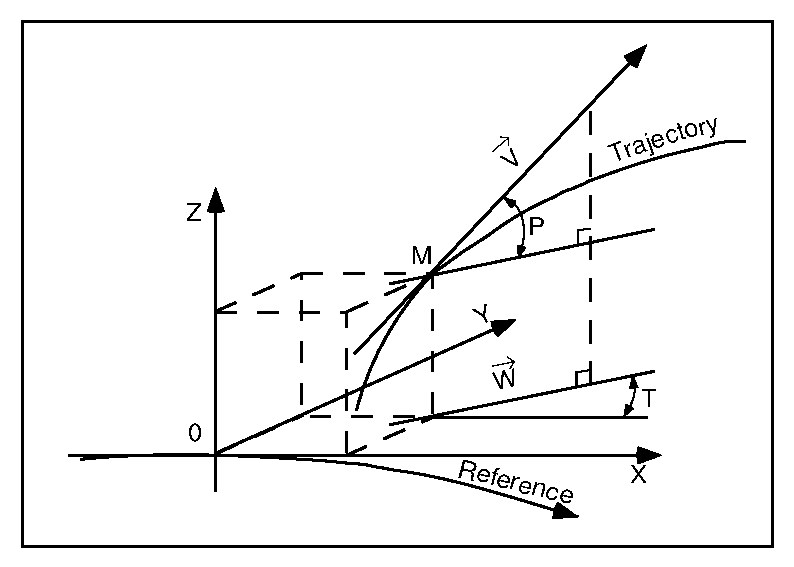
\includegraphics[width=14cm]{Fig1.ps}}
\hangcaption[Fig 1]{\label{fig1}Reference frame and coordinates ($Y$, 
$T$, $Z$, $P$) in \zgou.\\
$ OX$~:  in the plane of the reference curve in the direction of motion,\\										  %
$ OY$~:  in the plane of the reference curve, normal to $OX$,\\
$ OZ$~:  orthogonal to the $(X, Y)$ plane,\\				  
$ \vec{W}$~:  projection of the velocity, $ \vec	v $, in	the	$(X, Y)$ plane,\\									  %
$ T$  =	 angle between $\vec{W}$ and the  $X$-axis,\\
$ P$  =	 angle between $\vec{W}$ and $	\vec  v	$. } 
\end{figure}
\vspace{.3cm}



Taking
\begin{equation}
\vec  u = \frac{\vec  v }{v},\quad
    	ds = v\,dt,\quad
		\vec  u^{\,\prime}  =\frac{d\vec  u }{ds},\quad
			 m\vec  v = mv\vec  u = q\, \Br \, \vec  u \label{eq2-2-2}
\end{equation}
 where $ \Br $ is the rigidity of the particle, this equation can be rewritten 

\begin{equation}
(\Br )^\prime  \vec  u+\Br \,\vec  u^{\,\prime}  
	=  \frac{\vec  e }{v}  + \vec  u  \times   \vec  b   \label{eq2-2-3}
\end{equation}

\noindent From position $ \vec  R(M_0) $ and unit velocity $ \vec  u(M_0) $ at
point $ M_0 $, position $ \vec  R(M_1) $ and unit velocity $ \vec  u(M_1) $ 
at point $ M_1 $ following a 
displacement  $ \Delta s $, are obtained from truncated Taylor expansions (Fig.~\ref{fig2})  

\begin{equation}
\begin{aligned}
\vec  R(M_1)  &  \approx  \vec  R(M_0) + \vec  u(M_0)\, \Delta s+ \vec  u^{\,\prime} (M_0)\,
	\dfrac{\Delta s^2 }{2!}  +  ...+ \vec  u^{\cinqprime} (M_0)\,
	\dfrac{\Delta s^6 }{6!} \\
\vec  u(M_1) & \approx  \vec u(M_0)  + \vec  u^{\,\prime} (M_0)\,\Delta s  + \vec  u^{\,\prime\prime} (M_0)\,
	\dfrac{\Delta s^2 }{2!}  +   ...+ \vec  u^{\cinqprime} (M_0)\,
	\dfrac{\Delta s^5 }{5!} 
\end{aligned}\label{eq2-2-4}
\end{equation}

\noindent The rigidity at $ M_1 $ is obtained in the same way from
\begin{equation}
 (\Br )(M_1) \approx (\Br )(M_0)+(\Br )^\prime (M_0)\Delta s+...+
	(\Br)^{\quaprime} (M_0) \frac{\Delta s^4 }{4!}   	\label{eq2-2-5}
\end{equation}

\noindent The equation of time of flight is written in a similar manner 
\begin{equation}
 T(M_1) \approx   T(M_0) +   \frac{dT}{ds}(M_0)\, \Delta s+ \frac{d^2T}{ds^2} (M_0)\,\frac{\Delta s^2}{2} + 
     \frac{d^3T}{ds^3} (M_0)\,\frac{\Delta s^3}{3!} + \frac{d^4T}{ds^4} (M_0)\,\frac{\Delta s^4}{4!} 	\label{eq2-2-Time}
\end{equation}


\noindent The derivatives $\vec  u^{(n)} = \dfrac{d^n\vec  u}{ds^n}$ and 
$ (\Br )^{(n)} = \dfrac{d^n(\Br )}{ds^n} $
involved in these expressions are calculated as described in the next sections. 
For the sake of computing speed, three distinct software procedures are involved, depending on 
whether $\vec e$ or $\vec  b$ is zero, or $ \vec e$ and $ \vec b$ are 
both non-zero.

%%%%%%%%%%%%%%%%%%%%figure%%%%%%%%%%%%%%%%%%%%%
\begin{figure}[H]
%\vspace{10 truecm}
%%%Figure 2~: 
\centerline{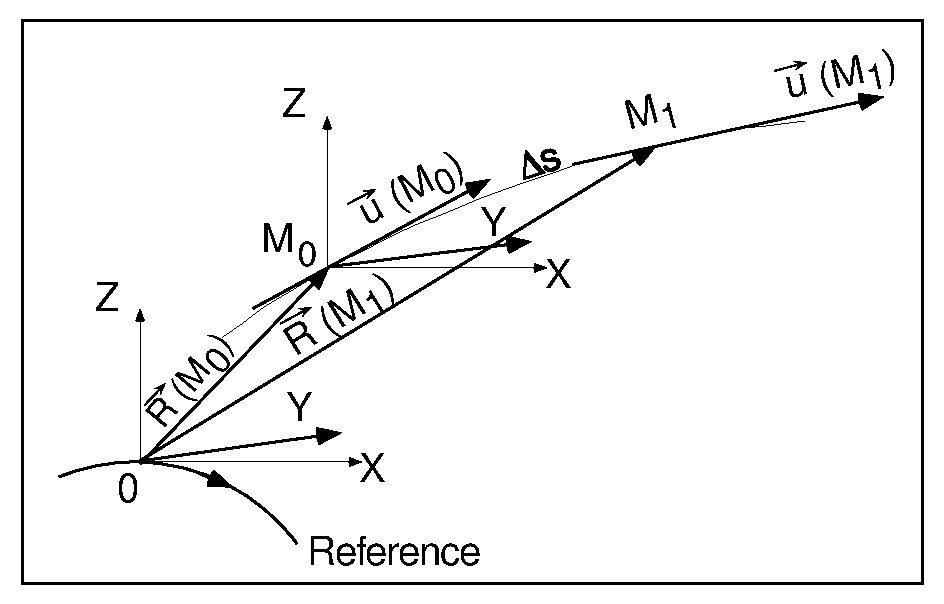
\includegraphics[width=14cm]{Fig2.ps}}
\hangcaption{\label{fig2}Position and velocity of a particle in the reference frame.}
\end{figure}

\subsubsection{Integration in magnetic fields} \label{sec2.2.1}  %% 2.2.1.

Admitting that $ \vec  e=0, $ and noting $ \vec B=\dfrac{\vec  b}{\Br} $, 
eq.~(\ref{eq2-2-3}) 
reduces to 
$$ \vec  u^{\,\prime}  = \vec  u  \times  \vec  B $$

\noindent The successive derivatives $\vec  u^{(n)} = \dfrac{d^n\vec  u }{ds^n} $ of 
$ \vec  u $ needed in the Taylor expansions (eqs.~\ref{eq2-2-4}) are calculated by differentiating 
$ \vec  u^{\,\prime}            =\vec  u  \times  \vec  B$ 

\begin{equation}
	\begin{aligned}
		\vec  u^{\,\prime\prime}
		         &   =   \vec  u^{\,\prime}   \times   \vec  B + \vec  u  \times  
		         \vec B^{\,\prime} \\
		\vec u^{\,\prime\prime\prime}
		         & = \vec  u^{\,\prime\prime}   \times   \vec  B 
		         + 2\vec  u^{\,\prime}  \times   \vec  B^{\,\prime}  
		         + \vec  u \times  \vec  B^{\,\prime\prime} \\
		\vec u^{\quaprime} 
		         &   =  \vec u^{\,\prime\prime\prime}  \times   \vec  B 
		         + 3\vec  u^{\,\prime\prime}   \times  \vec  B^{\,\prime}  
		         + 3\vec  u^{\,\prime}   \times   \vec  B^{\,\prime\prime}   
		         +\vec	u  \times  \vec  B^{\,\prime\prime\prime} \\
		\vec  u^{\cinqprime}
		         &  =  \vec u^{\quaprime}  \times \vec  B 
		         + 4\vec u^{\,\prime\prime\prime}  \times  \vec  B^{\,\prime}  
		         + 6\vec  u^{\,\prime\prime} \times   \vec  B^{\,\prime\prime}  
		         + 4\vec  u^{\,\prime}   \times   \vec B^{\,\prime\prime\prime} 
		         + \vec  u  \times   \vec  B^{\quaprime}
	\end{aligned}
	\label{eq2-2-6}
\end{equation}
%
 where $ \vec  B^{(n)} = \dfrac{d^n\vec  B}{ds^n}$. 

\noindent From $ d\vec  B = \dfrac{\partial\vec  B}{\partial X}\, dX
     +\dfrac{\partial\vec  B}{\partial Y}\, dY+
     \dfrac{\partial\vec  B}{\partial Z}\, dZ
     = \sum_{i=1,3}\dfrac{\partial\vec  B}{\partial X_i}\, dX_i$,  
and by successive differentiation, we get 

 \begin{equation}
	 \begin{aligned}
		 \vec  B^{\,\prime} =
		        &   \sum_i  \dfrac{\partial\vec  B}{\partial X_i}\, u_i \\
		 \vec  B^{\,\prime\prime} =
		        &  \sum_{ij}\dfrac{\partial^2\vec  B}{\partial X_i\partial X_j} 
		        \, u_i u_j+ \sum_i \dfrac{\partial\vec  B}{\partial X_i} \,u^{\,\prime}_i\\
		\vec  B^{\,\prime\prime\prime}  =
		        &  \sum_{ijk} \dfrac{\partial^3\vec  B}{\partial X_i\partial X_j\partial X_k}
		           \, u_i u_j u_k 
		           + 3 \sum_{ij} \dfrac{\partial^ 2\vec  B}{\partial X_i\partial X_j} \,u^{\prime}_i
		           u_j 
		           + \sum_i\frac{\partial\vec  B}{\partial X_i} \, u^{\prime\prime}_i \\
		\vec B^{\quaprime}  = 
		        & \sum_{ijkl} \dfrac{\partial^ 4\vec  B}{\partial X_i\partial X_j\partial
		           X_k\partial X_l} \,u_i u_j u_k u_l 
		           + 6 \sum_{ijk}  \dfrac{\partial^ 3\vec  B}{\partial X_i\partial X_j\partial X_k} \,
		           u^{\prime}_i u_j u_k \\
		 %
		        &
		        +  4 \sum_{ij} \dfrac{\partial^ 2\vec  B}{\partial X_i\partial X_j}\,
		         u^{\prime\prime}_i u_j
		         + 3 \sum_{ij} \dfrac{\partial^ 2\vec  B}{\partial X_i\partial X_j}\,
		         u^{\prime}_i u^{\prime}_j 
		         + \sum_i \dfrac{\partial\vec  B}{\partial X_i}\, u^{\prime\prime \prime}_i 
	 \end{aligned}
 	\label{eq2-2-7}
 \end{equation} 
 
 \noindent From the knowledge of $ \vec  u(M_0) $ and $ \vec  B(M_0) $ at point
$ M_0 $ of the 
trajectory, we calculate alternately the derivatives of $ \vec  u(M_0) $ and 
$ \vec  B(M_0) $, by means of eqs.~(\ref{eq2-2-6}) and (\ref{eq2-2-7}), and inject it in 
eq.~(\ref{eq2-2-4}) to get 
$ \vec  R(M_1) $ and $ \vec  u(M_1) $.

\subsubsection[Integration in electric fields]%
       {Integration in electric fields~\protect\cite{Biblio6}}
        \label{sec2.2.2} %%%% 2.2.2.[3]

Admitting that $ \vec  b=0, $ eq.~(\ref{eq2-2-3}) reduces to 

\begin{equation}
	(\Br )^\prime\vec  u + \Br\vec  u^{\,\prime} = \dfrac{\vec  e}{ v}
	\label{eq2-2-8}
\end{equation} 
%
which, by successive differentiations, gives the recursive relations

\begin{equation}
	\begin{array}{l}
		(\Br )^\prime\vec  u + \Br\vec  u^{\,\prime}   = \dfrac{\vec e}{ v}\\
		 (\Br )^{\prime\prime}\vec  u + 2 (\Br)^\prime \vec  u^{\,\prime} 
		     +\Br\vec  u^{\,\prime\prime}   = \left(\dfrac{1}{v}\right)^\prime\vec  e 
		         + \dfrac{\vec  e^{\,\prime}}{v} \\
		(\Br)^{\prime\prime\prime}\vec  u + 3(\Br)^{\prime\prime}\vec  u^{\,\prime}
		      + 3(\Br)^\prime \vec  u^{\,\prime\prime} 
		      +\Br\vec  u^{\prime\prime\prime}   =
		      \left(\dfrac{1}{ v}\right)^{\prime\prime}\vec  e +
		      2\left( \dfrac{1}{v}\right)^\prime \vec  e^{\,\prime} 
		      +\left(\dfrac{1}{v}\right)\, \vec  e^{\,\prime\prime}\\
		(\Br )^{\quaprime} \vec u + 4(\Br)^{\prime\prime\prime} \vec  u^{\,\prime} 
		      + 6(\Br)^{\prime\prime}\vec  u^{\,\prime\prime} 
		      +4 (\Br)^\prime\vec  u^{\,\prime\prime\prime} 
		      +\Br\vec  u^{\quaprime} = \\
		%
		\hphantom{(\Br )^{\quaprime} \vec u}
		\left(\dfrac{1}{v}\right)^{\prime\prime\prime}\vec e
		      +3\left(\dfrac{1}{v}\right)^{\prime\prime}\vec  e^{\,\prime} 
		      +3\left(\dfrac{1}{ v}\right)^\prime\vec e^{\,\prime\prime} +
		      \dfrac{1}{v} \,\vec  e^{\,\prime\prime\prime}
	\end{array}
	\label{eq2-2-9}
\end{equation} 
%
that provide the derivatives $ \dfrac{d^n\vec  u}{ds^n}$ needed in the Taylor 
expansions~(eq.~\ref{eq2-2-4})

\begin{equation}
	\begin{aligned}
		\vec  u^{\,\prime} 
		       & =  \left(\dfrac{1}{v}\right)\, \vec  E 
		             - \dfrac{(\Br )^\prime}{\Br} \, \vec  u\\
		\vec u^{\,\prime\prime} 
		       & =  \left(\dfrac{1}{v}\right)^\prime \vec  E 
		            + \left(\dfrac{1}{v}\right)\, \vec  E^{\,\prime} 
		            \mid_{ \Br}  -2 \dfrac{(\Br )^\prime }{ \Br} 
		             \vec  u^{\,\prime} -
		             \dfrac{(\Br)^{\prime\prime}}{\Br}  \vec  u \\
	    \vec  u^{\,\prime\prime\prime} 
	           &  = \left( \dfrac{1}{v}\right)^{\prime\prime}\vec  E
	               +2\left(\dfrac{1}{v}\right)^\prime \vec  E^{\,\prime} 
	               \mid_{ \Br} +\dfrac{1}{v} \vec  E^{\,\prime\prime} 
	               \mid_{ \Br} -3 \dfrac{(\Br )^\prime }{\Br}  \vec  u^{\,\prime\prime} 
	               -3 \dfrac{(\Br )^{\prime\prime}}{\Br}  \vec u^{\,\prime} 
	               - \dfrac{(\Br )^{\prime\prime\prime} }{\Br}  \vec  u \\
		\vec  u^{\quaprime}
		      & =  \left(\dfrac{1}{v}\right)^{\prime\prime\prime}  \vec  E 
		           +3\left(\dfrac{1}{v}\right)^{\prime\prime}\vec E^{\,\prime} \mid_{ \Br} 
		           +3\left( \dfrac{1}{v}\right)^\prime \vec  E^{\,\prime\prime} \mid_{\Br} 
		           +\left(\dfrac{1}{v}\right)\,\vec  E^{\,\prime\prime\prime} \mid_{\Br} \\
		%
		      &  \qquad -4 \dfrac{(\Br )^\prime }{\Br}  \vec  u^{\,\prime\prime\prime} 
		           -6 \dfrac{(\Br )^{\prime\prime}}{\Br}  \vec  u^{\,\prime\prime} 
		           -4 \dfrac{(\Br )^{\prime\prime\prime} }{\Br}  \vec  u^{\,\prime} 
		           - \dfrac{(\Br )^{\quaprime}}{\Br}  \vec  u \\
             \vec  u^{\cinqprime}
		      & =  \left(\dfrac{1}{v}\right)^{\quaprime}  \vec  E 
		           +4\left(\dfrac{1}{v}\right)^{\prime\prime\prime}\vec E^{\,\prime} \mid_{ \Br} 
		           +6\left(\dfrac{1}{v}\right)^{\prime\prime}\vec E^{\,\prime\prime} \mid_{ \Br} 
		           +4\left( \dfrac{1}{v}\right)^\prime \vec  E^{\,\prime\prime\prime} \mid_{\Br} 
		           +\left(\dfrac{1}{v}\right)\,\vec  E^{\,\quaprime} \mid_{\Br} \\
		%
		      &  \qquad -5 \dfrac{(\Br )^\prime }{\Br}  \vec  u^{\,\quaprime} 
		           -10 \dfrac{(\Br )^{\prime\prime}}{\Br}  \vec  u^{\,\prime\prime\prime} 
		           -10 \dfrac{(\Br )^{\prime\prime\prime}}{\Br}  \vec  u^{\,\prime\prime} 
		           -5 \dfrac{(\Br )^{\quaprime} }{\Br}  \vec  u^{\,\prime} 
		           - \dfrac{(\Br )^{\cinqprime}}{\Br}  \vec  u	\end{aligned}
	\label{eq2-2-10}
\end{equation}
%
where $ \vec  E=\dfrac{\vec  e}{\Br} $, and $(~)^{(n)}\mid_{ \Br} $ 
denotes differentiation at constant $ \Br$~:  
$ \vec E^{(n)}\mid_{ \Br} =   \dfrac{ 1}{\Br} \dfrac{d^n\vec  e }{ds^n}$.  
These derivatives of the electric field are obtained from the total 
derivative

 \begin{equation}
	 d\vec  E = \dfrac{\partial\vec  E}{\partial X}\, dX + 
	 \dfrac{\partial\vec  E }{\partial Y} \, dY + 
	 \dfrac{\partial\vec  E }{ \partial Z} \, dZ
 	\label{eq2-2-11}
 \end{equation} 
%
 by successive differentiations

\begin{equation}
	\begin{aligned}
		\vec  E^{\,\prime} 
		     & =   \sum_ i \dfrac{\partial\vec  E}{\partial X_i} \,u_i \\
		\vec  E^{\,\prime\prime} 
		     & =  \sum_{ij} \dfrac{\partial^ 2\vec  E}{\partial X_i\partial X_j}\, u_i u_j 
		       +\sum_i \dfrac{\partial\vec  E}{\partial X_i} \,u^{\prime}_i \\
		\vec  E^{\,\prime\prime\prime} 
		     & =  \sum_{ijk} \dfrac{\partial^ 3\vec  E }{\partial X_i\partial X_j\partial X_k}\,
		        u_i u_j u_k 
		        + 3 \sum_{ij} \dfrac{\partial^ 2\vec  E}{\partial X_i\partial X_j} \,u^{\prime}_i u_j 
		        + \sum_i \dfrac{\partial\vec  E}{\partial X_i} \,u^{\prime\prime}_i 
	\end{aligned}
	\label{eq2-2-12}
\end{equation}

\noindent etc. as in eq.~\ref{eq2-2-7}. 
These eqs.~(\ref{eq2-2-10}), as well as the calculation of the rigidity, following 
eq.~(\ref{eq2-2-5}), involve 
derivatives $ (\Br)^{(n)} =  \dfrac{ d^n(\Br )}{ds^n} $, which are obtained in the following way. 
Considering that 

\begin{equation}
	\dfrac{dp^2 }{dt} = \dfrac{d\vec  p^{2} }{ dt}
	\quad \text{\emph{i.e.,}} \quad 
	\dfrac{dp}{dt}\, p = \dfrac{d\vec  p}{dt} \vec  p
	\label{eq2-2-13}
\end{equation}
%
with $ \dfrac{ d\vec  p }{ dt} = q\,(\vec  e +\vec v\times\vec  b) $ 
(eq.~\ref{eq2-2-1}), we obtain

\begin{equation}
	\dfrac{dp }{ dt} \,p =  q\,(\vec  e + v\times\vec  b)\cdot \vec  p =q\vec  e \cdot \vec  p
	\label{eq2-2-14}
\end{equation}
%
since $ (\vec  v\times\vec  b) \cdot \vec  p=0$.  Normalizing as
previously with $ \vec  p=p\vec  u=q\Br\vec  u $ and $ ds=vdt$,  and 
by successive differentiations, eq.~(\ref{eq2-2-14}) leads to the $ (\Br )^{(n)} $

\begin{equation}
	\begin{aligned}
		(\Br )^\prime 
		      & =  \dfrac{ 1 }{ v}\, (\vec  e \cdot \vec  u) \\
		(\Br)^{\prime\prime}
		      & =  \left(\dfrac{1 }{ v}\right)^\prime
		        (\vec  e \cdot \vec  u) +
		        \dfrac{1 }{ v}\, (\vec  e\cdot\vec  u)^\prime \\
		(\Br )^{\prime\prime\prime}
		      & =  \left(\dfrac{1 }{ v}\right)^{\prime\prime} (\vec  e\cdot\vec  u)
		        +2\left(\dfrac{1 }{v}\right)^\prime (\vec  e\cdot\vec  u)^\prime 
		        +\dfrac{1 }{ v}\, (\vec  e\cdot\vec u)^{\prime\prime} \\
	    (\Br )^{\quaprime} 
	          & =  \left(\dfrac{1 }{v}\right)^{\prime\prime\prime} (\vec  e\cdot\vec  u)
	            +3\left(\dfrac{1 }{ v}\right)^{\prime\prime}(\vec  e\cdot\vec  u)^\prime 
	            +3\left(\dfrac{1 }{ v}\right)^\prime (\vec  e\cdot\vec u)^{\prime\prime} 
	            + \dfrac{1 }{ v}\, (\vec  e\cdot\vec  u)^{\prime\prime\prime}
	\end{aligned}
	\label{eq2-2-15}
\end{equation}

\noindent Note that the derivatives $ (\vec  e \cdot \vec  u)^{(n)} = 
\dfrac{ d^n(\vec e\cdot\vec  u) }{ ds^n} $ can be related to the derivatives of the 
kinetic energy $ W $ by $dW = \dfrac{d\vec  p }{ dt} \cdot\vec  v\, dt = q\vec  e\cdot\vec  v\, dt $
which leads to

\begin{equation}
	\dfrac{ d^{n+1}W }{ds^{n+1}} = q \dfrac{ d^n (\vec  e\cdot\vec  u) }{ ds^n}
	\label{eq2-2-16}
\end{equation}


\noindent Finally, the derivatives $ \left(\dfrac{ 1 }{ v}\right)^{(n)} =
\dfrac{ d^n \left(\dfrac{1 }{ v}\right) }{ ds^n} $ involved in 
eqs.~(\ref{eq2-2-10},\ref{eq2-2-15}) are 
obtained from $ p=\dfrac{ v }{ c} \dfrac{ W+m_0 c^2 }{ c} $,
 ($m_0$ is the rest mass) by successive differentiations, that give the recursive relations

\begin{equation}
	\begin{aligned}
		 \left(\dfrac{1}{ v}\right) 
		   & =   \dfrac{ 1 }{ c^2} \, 
		     \dfrac{W+m_0 c^2 }{ q\Br}\\
		 \left(\dfrac{1 }{ v}\right)^\prime 
		   & =  \dfrac{ 1 }{ c^2}\,
		     \dfrac{(\vec  e\cdot\vec  u) }{ \Br} 
		      - \dfrac{1 }{ v} \dfrac{(\Br )^\prime }{ \Br}\\
		 \left(\dfrac{1 }{ v}\right)^{\prime\prime}
		   & = 	\dfrac{ 1 }{ c^2} \,
		     \dfrac{(\vec  e\cdot\vec  u)^\prime }{ \Br}  
		     - 2\left(\dfrac{1}{v}\right)^\prime \dfrac{ (\Br )^\prime }{ \Br}  
		     - \dfrac{1 }{ v}\, \dfrac{(\Br)^{\prime\prime} }{ \Br}\\
		 \left(\dfrac{1 }{v}\right)^{\prime\prime\prime} 
		   & = \dfrac{ 1 }{c^2}\, \dfrac{(\vec  e\cdot\vec  u)^{\prime\prime} }{ \Br}  
		     -3\left(\dfrac{1 }{v}\right)^{\prime\prime}  \dfrac{(\Br )^\prime }{ \Br}  
		     -3\left(\dfrac{1 }{v}\right)^\prime \dfrac{(\Br )^{\prime\prime} }{ \Br}  
		     - \dfrac{1 }{ v}\, \dfrac{(\Br)^{\prime\prime\prime} }{ \Br}
	\end{aligned}
	\label{eq2-2-17}
\end{equation}



 \subsubsection{Integration in combined electric and magnetic fields} \label{sec2.2.3}%%%% 2.2.3.

 When both $ \vec  e $ and $ \vec  b $ are non-zero, the complete 
 eq.~(\ref{eq2-2-3}) must 
be considered. Recursive differentiations give the following relations 

\begin{equation}
	\begin{array}{l}
		(\Br )^\prime\vec  u+\Br\vec  u^{\,\prime} 
		     =  \dfrac{\vec e }{ v} + \vec  u \times  \vec  b \\
		(\Br)^{\prime\prime}\vec  u+ 2(\Br )^\prime\vec  u^{\,\prime} 
		  +\Br\vec u^{\,\prime\prime} 
		     = \left(\dfrac{1 }{ v}\right)^\prime\vec  e + \left(\dfrac{1 }{ v}\right)\,\vec  e^{\,\prime}
		       +(\vec  u\times\vec  b)^\prime \\
		(\Br)^{\prime\prime\prime}\vec  u +3(\Br )^{\prime\prime}\vec  u^{\,\prime}
		  +3 (\Br )^\prime\vec  u^{\,\prime\prime} +\Br\vec  u^{\,\prime\prime\prime}
		     =  \left(\dfrac{1 }{ v}\right)^{\prime\prime}\vec  e
		     + 2\left(\dfrac{1 }{ v}\right)^\prime\vec  e^{\,\prime}
		     +\left(\dfrac{1 }{ v}\right)\, \vec  e^{\,\prime\prime} 
		     +(\vec  u\times\vec  b)^{\prime\prime} \\
		(\Br )^{\quaprime}\vec  u + 4(\Br )^{\prime\prime\prime}\vec  u^{\,\prime} 
		  +6 (\Br )^{\prime\prime}\vec u^{\,\prime\prime} +4(\Br )^\prime
		  \vec  u^{\,\prime\prime\prime} +\Br\vec u^{\quaprime} = \\
		%
		\hphantom{(\Br )^{\quaprime}\vec  u}
		 \left(\dfrac{1 }{ v}\right)^{\prime\prime\prime}\vec  e 
		   + 3\left(\dfrac{1 }{ v}\right)^{\prime\prime}\vec e^{\,\prime} 
		   +3\left(\dfrac{1 }{ v}\right)^\prime\vec  e^{\,\prime\prime} 
		   +\dfrac{1 }{ v} \vec e^{\,\prime\prime\prime} +(\vec  u\times\vec  b)^{\prime\prime\prime}
	\end{array} 
	\label{eq2-2-18}
\end{equation}
%
 that provide the derivatives $ \dfrac{ d^n\vec  u }{ ds^n}$ needed in the Taylor 
 expansions~(\ref{eq2-2-4})  

\begin{equation}
	\begin{aligned}
		\vec  u^{\,\prime}    
		   & =  \left(\dfrac{1 }{ v}\right)\, \vec  E
		      + (\vec  u\times\vec  B) - 
		      \dfrac{(\Br )^\prime }{ \Br}  \vec  u \\
		\vec  u^{\,\prime\prime}  
		   &   =  \left(\dfrac{1 }{ v}\right)^\prime\vec  E 
		      + \left(\dfrac{1 }{ v}\right)\,\vec  E{^{\,\prime}} \mid_{ \Br} 
		      +(\vec u\times\vec  B^{\,\prime} )^\prime \mid_{ \Br}
		      -2 \dfrac{(\Br )^\prime }{ \Br} \vec  u^{\,\prime} 
		      - \dfrac{(\Br )^{\prime\prime} }{ \Br}  \vec  u \\
		\vec  u^{\,\prime\prime\prime} 
		   &  =   \left(\dfrac{1 }{v}\right)^{\prime\prime}\vec  E
		      +2 \left(\dfrac{1 }{ v}\right)^\prime\vec  E^{\,\prime} \mid_{ \Br}
		      +\dfrac{1 }{ v} \vec  E^{\,\prime\prime} \mid_{ \Br} 
		      +(\vec  u\times\vec B)^{\prime\prime} \mid_{ \Br}  
		      -3 \dfrac{(\Br )^\prime }{ \Br}  \vec u^{\,\prime\prime} 
		      -3 \dfrac{(\Br )^{\prime\prime} }{ \Br}  \vec  u^{\,\prime}
		      - \dfrac{(\Br )^{\prime\prime\prime} }{ \Br}  \vec  u \\
		\vec  u^{\quaprime}  
		   & =    \left(\dfrac{1}{ v}\right)^{\prime\prime\prime}  \vec  E
		      +3 \left(\dfrac{1 }{ v}\right)^{\prime\prime}\vec E^{\,\prime} \mid_{ \Br} 
		      +3( \dfrac{1 }{ v})^\prime\vec  E^{\,\prime\prime} \mid_{\Br} 
		      +\left(\dfrac{1 }{ v}\right)\, \vec  E^{\,\prime\prime\prime} \mid_{ \Br} \\
		%
		  &  \quad + (\vec  u\times\vec B)^{\prime\prime\prime} \mid_{ \Br} 
		      -4 \dfrac{(\Br )^\prime }{ \Br}  \vec u^{\,\prime\prime\prime} 
		      -6 \dfrac{(\Br )^{\prime\prime} }{ \Br}  \vec u^{\,\prime\prime} 
		      -4 \dfrac{(\Br )^{\prime\prime\prime} }{ \Br}  \vec  u^{\,\prime} 
		      - \dfrac{(\Br )^{\quaprime} }{ \Br}  \vec  u
	\end{aligned}
	\label{eq2-2-19}
\end{equation}
%
where $ \vec  E =  \dfrac{\vec  e }{ \Br} $, 
$ \vec  B =\dfrac{\vec  b }{ \Br} $, and $^{(n)}\mid_{ \Br} $ denotes
differentiation at constant $ \Br$ 
 \begin{equation}
	 \vec  E^{(n)}\mid_{ \Br} = \dfrac{1 }{ \Br}  \dfrac{d^n\vec  e }{ ds^n}
	 \quad \text{and} \quad 
	 (\vec  u\times\vec  B)^{(n)}\mid_{ \Br} = \dfrac{1}{\Br}  (\vec  u\times\vec  b)^{(n)}.
 	\label{eq2-2-20}
 \end{equation}

\noindent These derivatives $ \vec  E^{(n)} $ and $ \vec  B^{(n)} $ of the
electric and magnetic fields are 
calculated from the vector fields $ \vec  E(X,Y,Z)$,  $ \vec  B(X,Y,Z) $ and
their derivatives  
$ \dfrac{ \partial^{i+j+k} \vec  E }{ \partial X^i \partial Y^j\partial Z^k} $ 
and 
$ \dfrac{ \partial^{ i+j+k} \vec  B }{ \partial X^i \partial Y^j \partial Z^k}$, 
following eqs.~(\ref{eq2-2-7}) and (\ref{eq2-2-12}).


\subsubsection{Calculation of the time of flight \label{CalcTOF}} 

The time of flight  eq.~(\ref{eq2-2-Time}) involves the derivatives 
$dT/ds=1/v$, $d^2T/ds^2=d(1/v)/ds$, etc. that are obtained from eq.~(\ref{eq2-2-17}). In the absence of 
electric field   eq.~(\ref{eq2-2-6}) however reduces to the simple form 
 \begin{equation}
T(M_1) =   T(M_0) +  \Delta s/v  
 \end{equation}


\subsection{Calculation of  $ \vec B $ and its Derivatives}\label{sec2.3}    %%%%%  2.3.

\noindent $ \vec  B(X,Y,Z) $ and 
derivatives are calculated in various ways, depending  whether field maps or analytic
 representations of optical elements are  used. The  basic means are the following. 
 
\subsubsection[Extrapolation from  1-D axial field map]%
      {Extrapolation from  1-D axial field map~\protect\cite{Biblio3}}  
       \label{sec2.3.1} %%%%%  2.3.1.  [3]


 A cylindrically symmetric field (e.g., using \textsl{BREVOL}\index{BREVOL}) can be described
by an axial 1-D field map of its longitudinal component $ B_X(X,r=0) $
 $(r=(Y^2+Z^2)^{1/2})$,  
while the radial component on axis $ B_r(X,r=0) $ is assumed to be zero. $ B_X(X,r=0) $ is obtained 
at any point along the $ X$-axis by a 
polynomial interpolation from the map mesh (see section \ref{sec2.4.1}).  %%% ref 
Then the field components $ B_X(X,r)$,  $ B_r(X,r) $ at the position of the particle, 
$(X,r) $ are obtained from Taylor expansions truncated at  the fifth order in $ r $ (hence, up to 
the fifth order derivative $ \dfrac{ \partial^ 5B_X }{ \partial X^5} \,(X,0)$),  
assuming cylindrical symmetry 
 \begin{equation}
	 \begin{aligned}
		 B_X(X,r) 
		   &   =  B_X(X,0) -
		       \dfrac{r^2 }{ 4} \dfrac{\partial^ 2B_X }{ \partial X^2}\, (X,0)
		       + \dfrac{r^4 }{64} \dfrac{\partial^ 4B_X }{ \partial X^4} \,(X,0) \\
		 B_r(X,r)
		   & =    - \dfrac{r }{ 2} \dfrac{\partial B_X }{ \partial X} \, (X,0) 
		       + \dfrac{r^3 }{ 16} \dfrac{\partial^ 3B_X }{ \partial X^3}\, (X,0)
		       - \dfrac{r^5 }{384} \dfrac{\partial^ 5B_X }{ \partial X^5}\, (X,0) 
	 \end{aligned}
 	\label{eq2-3-1}
 \end{equation}
By differentiation with respect to $ X $ and $ r$,  up to the second
order, these expressions provide the derivatives of $ \vec  B(X,r)$.  Finally a conversion
from the $ (X,r) $ coordinates to the $ (X,Y,Z) $ Cartesian coordinates of \zgou\ is 
performed, thus providing the expressions 
$ \dfrac{ \partial^{i+j+k} \vec  B }{\partial X^i\partial Y^j\partial Z^k} $ needed in the 
eq.~(\ref{eq2-2-7}). 

\subsubsection{Extrapolation from Median Plane Fields} \label{sec2.3.2} %%%%%%  2.3.2.  

In the median plane, $ B_Z(X,Y,0)$, and its 
derivatives with respect to $ X $ or $ Y$, may be calculated  from analytical
models (e.g.\ in Venus magnet - \textsl{VENUS\index{VENUS}}, and sharp edge 
multipoles  \textsl{SEXQUAD\index{SEXQUAD}}   and \textsl{QUADISEX\index{QUADISEX}}) or numerically by
polynomial interpolation from 2-D field maps (e.g.\ \textsl{CARTEMES\index{CARTEMES}, 
TOSCA\index{TOSCA}}).  

\smallskip

\noindent Median plane antisymmetry is assumed, which results in 
\begin{equation}
	\begin{aligned}
		B_X(X,Y,0)  &  =   0 \\
		B_Y(X,Y,0) & =  0 \\
		B_X(X,Y,Z)  & =  -B_X(X,Y,-Z) \\
		B_Y(X,Y,Z)  &  =  -B_Y(X,Y,-Z) \\
		B_Z(X,Y,Z) & =   B_Z(X,Y,-Z) 
	\end{aligned}
	\label{eq2-3-2}
\end{equation}
Accomodated with Maxwell's equations, this results 
 in  Taylor expansions below,  for the three components of $ \vec  B $ (here, 
$ B $ stands for $ B_Z(X,Y,0)$) 
\begin{equation}
	\begin{aligned}
		B_X(X,Y,Z) 
		      & =   Z \dfrac{\partial B }{ \partial X} - \dfrac{Z^3 }{ 6} 
		        \left(  \dfrac{\partial^ 3B }{\partial X^3} 
		           + \dfrac{\partial^ 3B }{ \partial X\partial Y^2} \right) \\
		B_Y(X,Y,Z)
		      & =  Z \dfrac{\partial B }{ \partial Y} - \dfrac{Z^3}{ 6} 
		        \left(\dfrac{\partial^ 3B }{\partial X^2\partial Y} 
		           + \dfrac{\partial^ 3B}{ \partial Y^3} \right) \\
		B_Z(X,Y,Z) 
		      & =  B - \dfrac{Z^2 }{ 2} 
		        \left(  \dfrac{\partial^ 2B }{ \partial X^2} 
		           + \dfrac{\partial^ 2B}{\partial Y^2} \right) 
		        + \dfrac{Z^4 }{ 24} 
		        \left( \dfrac{\partial^ 4B }{\partial X^4} 
		           + 2 \dfrac{\partial^ 4B }{ \partial X^2\partial Y^2} 
		           + \dfrac{\partial^4B }{ \partial Y^4} \right)
	\end{aligned}
	\label{eq2-3-3}
\end{equation}
 which are then differentiated one by one with respect to $ X$, $Y$, 
or $ Z$, up to second or fourth order (depending on optical element or 
\textsl{IORDRE\index{IORDRE}} option, see section \ref{sec2.4.2}) so as to get the expressions
 involved in eq.~(\ref{eq2-2-7}). 
 


\subsubsection{Extrapolation from arbitrary 2-D Field Maps}\label{sec2.3.3}

2-D field maps that give the three components $ B_X(X,Y,Z_0)$,  
$B_Y(X,Y,Z_0) $ and $ B_Z(X,Y,Z_0) $ 
at each node $ (X,Y) $ of a $ Z_0 $ $ Z$-elevation map may be used. 
$ \vec  B$ and its derivatives at any point $ (X,Y,Z) $ are calculated by polynomial 
interpolation  followed by Taylor expansions in $ Z$,
without any hypothesis of symmetries (see section~\ref{sec2.4.3} and keywords 
\textsl{MAP2D}, \textsl{MAP2D-E}\index{MAP2D}\index{MAP2D-E}).

\subsubsection[Interpolation in 3-D Field Maps]%
        {Interpolation in 3-D Field Maps~\protect\cite{Biblio4}}
           \label{sec2.3.4} %%%% 2.3.4.  [4]

In 3-D field maps $ \vec  B $ and its derivatives up to the second
order with respect to $ X$, $Y$,  or $ Z $ are calculated by means of a second order polynomial 
interpolation,  from  3-D  $ 3  \times  3 
 \times $ 3-point grid (see section~\ref{sec2.4.4}). 




\subsubsection{2-D Analytical Field Models and Extrapolation} 

Several optical elements such as \textsl{BEND\index{BEND}}, \textsl{WIENFILT\index{WIENFILT}} (that 
uses the \textsl{BEND} procedures), \textsl{QUADISEX\index{QUADISEX}}, \textsl{VENUS\index{VENUS}}, etc., 
are defined from the  expression of the field and derivatives in the median plane. 
3-D extrapolation of these off the median is drawn from Taylor expansions. 





 
\subsubsection{3-D Analytical Models of Fields} \label{sec2.3.5} 

In many optical elements such as \textsl{QUADRUPO\index{QUADRUPO}, SEXTUPOL\index{SEXTUPOL}, 
MULTIPOL\index{MULTIPOL}, EBMULT\index{EBMULT}},  etc.,  the three 
components of $ \vec  B $  and their derivatives with respect to $ X$, $Y $ 
or $ Z $ are obtained at any step along trajectories from analytical 
expression drawn from the scalar potential $ V(X,Y,Z) $ following 

 \begin{equation}
%	 \begin{alignedat}{3}
	 	 B_X = \dfrac{\partial V}{\partial X}, 
	 	    \quad B_Y = \dfrac{\partial V }{ \partial Y}, 
	 	     \quad B_Z = \dfrac{\partial V }{ \partial Z}, 
	 	  \quad \dfrac{\partial B_X }{ \partial X} = \dfrac{\partial^2V}{\partial X^2},
	 	     \quad \dfrac{\partial B_X}{\partial Y} 
	 	               = \dfrac{\partial^2V}{\partial X\partial Y},
	 	    \quad\text{etc.}
%	 \end{alignedat}
 	\label{eq2-3-4}
 \end{equation}

\paragraph{Multipoles}

\noindent The scalar potential used for the calculation of 
$ \dfrac{\partial^{i+j+k} \vec B_{n}(X,Y,Z)}{ \partial X^i\partial Y^i\partial 
Z^k}$ ($i+j+k= 0 \text{ to } 4$) in the case of 
 magnetic and electro-magnetic multipoles with $2n$ poles
(namely, \textsl{QUADRUPO}\index{QUADRUPO} ($n = 2$) to  
\textsl{DODECAPO}\index{DODECAPO} ($n=6$),   
\textsl{MULTIPOL}\index{MULTIPOL} ($n = 1$ to 10), 
\textsl{EBMULT}\index{EBMULT} ($n=1$ to 10))   is~\cite{Biblio5}              %%%%% [5] 

\begin{equation}
	V_n(X,Y,Z)=(n!)^2 
	  \left( \sum^{ \infty}_{ q=0}(-1)^q \,
	        \dfrac{G^{(2q)}(X)(Y^2+Z^2)^q }{ 4^q q!(n+q)!} \right) 
	  \left( \sum^ n_{m=0}\dfrac{sin \left(m \dfrac{\pi }{ 2} \right) Y^{n-m} Z^m }{ m!(n-m)!} \right) 
	\label{eq2-3-5}
\end{equation}
%
 where $ G(X) $ is the longitudinal gradient, defined at the entrance 
 or exit of the optical element by

 \begin{equation}
	 G(s) = \dfrac{G_0 }{ 1+ \exp(P(s))} , \quad G_0 = \dfrac{B_0 }{R^n_0} 
 	\label{eq2-3-6}
 \end{equation}
wherein 
$$ P(s) = C_0
	       +C_1 \left(  \dfrac{s }{ \lambda} \right) 
	       +C_2 \left( \dfrac{s }{ \lambda} \right)^2 
	       + C_3 \left( \dfrac{s }{ \lambda} \right)^3 
	       +C_4 \left( \dfrac{s }{ \lambda} \right)^4 
	       + C_5 \left(\dfrac{s }{ \lambda} \right)^5 $$ 
and $s$ is the distance to the EFB.
 
\paragraph{Skewed multipoles}

\noindent A multipole component with arbitrary order $n$ can be tilted independently of 
the others by an arbitrary 
angle $A_n$ around the $X$-axis. If so, the calculation of the field and derivatives in the 
rotated axis $ (X,Y_R,Z_R) $ is done in two steps. First, they are 
calculated at the rotated position $ (X,Y_R,Z_R)$,  in the $ (X,Y,Z) $ 
frame, as derived from  expression (\ref{eq2-3-5}) above. Second, $ \vec  B $ and 
its derivatives at $ (X,Y_R,Z_R) $ in the $ (X,Y,Z) $ frame are transformed 
to the rotated $ (X,Y_R,Z_R) $ frame by a rotation of the same angle 
$A_n$. 

In particular a skewed $2n$-pole component is created  by taking $A_n = \pi/2n$.



\subsection{Calculation of $ \vec B $ from Field Maps}  \label{seq2.4}

\subsubsection{1-D Axial Map, with Cylindrical Symmetry}  \label{sec2.4.1}

 Let $ B_i $ be the value of the longitudinal component $ B_X(X,r=0)$ of the 
field $ \vec  B$, at  node $ i $ of a uniform mesh that defines a 1-D
field map along the symmetry $ X$-axis, while $ B_r(X,r=0) $ is assumed to be zero 
$(r=(Y^2+Z^2)^{1/2})$. The field component $B_X(X,r=0) $ 
is calculated by a polynomial interpolation of the fifth degree in $ X$,  
using a 5~points grid centered at the node of the 1-D map which is closest 
to the actual coordinate $ X $ of the particle. 

\noindent The interpolation polynomial is

 \begin{equation}
	 B(X,0)=A_0 + A_1 X + A_2 X^2 + A_3 X^3 + A_4 X^4 + A_5 X^5 
 	\label{eq2-4-1}
 \end{equation}
 %
and the coefficients $ A_i $ are calculated by expressions that
minimize the quadratic sum
\medskip
 \begin{equation}
     S = \sum_i \left(B(X,0)-B_i \right)^2  
 	\label{eq2-4-2}
 \end{equation}

\noindent Namely, the source code contains the explicit analytical 
expressions of the coefficients $A_i$ solutions of the normal 
equations $\partial S / \partial A_i = 0$.

\noindent The derivatives $  \dfrac{ \partial^n B }{ \partial X^n}
(X,0) $ at the actual position $ X$,  as involved 
in eqs.~(\ref{eq2-3-1}), are then obtained by differentiation of the polynomial 
(\ref{eq2-4-1}), giving

\begin{equation}
	\begin{aligned}
		\dfrac{ \partial B }{ \partial X}\, (X,0) 
		  &  =  A_1 + 2 A_2 X + 3 A_3 X^2 + 4 A_4 X^3 + 5 A_5 X^4 \\
		\dfrac{\partial^2 B }{ \partial X^2}\, (X,0)  
		  & = 2 A_2 + 6 A_3 X + 12 A_4 X^2 + 20 A_5 X^3 \\
		\ldots & \\
		 \dfrac{\partial^5 B }{ \partial X^5}\, (X,0) 
		  & = 120 A_5 
	\end{aligned}
	\label{eq2-4-3}
\end{equation}
  
  
\subsubsection{2-D Median Plane Map, with Median Plane Antisymmetry} \label{sec2.4.2}

Let $ B_{ij} $ be the value of $ B_Z(X,Y,0) $ at the nodes of a mesh
which defines a 2-D field map in the ($ X,Y) $ plane while $ B_X(X,Y,0) $ and $ B_Y(X,Y,0) $
are assumed to be zero.  Such a map may have been built or measured 
in either Cartesian or polar coordinates.  Whenever polar coordinates are used, a
change to Cartesian coordinates (described below) provides the expression of 
$ \vec  B $ and its derivatives as involved in eq.~(\ref{eq2-2-7}). 

\noindent\zgou\ provides three types of polynomial
interpolation from the mesh (option \textsl{IORDRE\index{IORDRE}})~; namely, a second order interpolation, 
with either a 9- or a 25-point grid, or a fourth 
order interpolation with a 25-point  grid (Fig.~\ref{fig3}).  

\noindent If the 2-D field map is built up from  simulation, the grid simply
aims at interpolating the field at a given point from its 9 or 25~neighbors.  If 
the map results from measurements, the grid also smoothes field measurement 
fluctuations. 

\noindent The mesh may be defined in Cartesian coordinates, 
(Figs.~3A and 3B) or in polar coordinates (Fig.~~\ref{fig3}C).   

\noindent The interpolation grid is centered on the node which is closest to
the projection in  the ($ X,Y) $ plane of the actual point of the trajectory. 

\noindent The interpolation polynomial is 

 \begin{equation}
	 B(X,Y,0) = A_{00} + A_{10}X + A_{01}Y + A_{20}X^2 + A_{11}XY + A_{02}Y^2
 	\label{eq2-4-4}
 \end{equation}
 %
 in second order, or 

 \begin{equation}
	 \begin{aligned}
		 B(X,Y,0)  = 
		    & A_{00}+A_{10}X+A_{01}Y + A_{20}X^2 + A_{11}XY + A_{02}Y^2 \\
		%
		    & +  A_{30}X^3+A_{21}X^2Y + A_{12}XY^2 + A_{03}Y^3 \\
		%
		    & +  A_{40}X^4 + A_{31}X^3Y + A_{22}X^2Y^2 +A_{13}XY^3 + A_{04}Y^4 
	 \end{aligned}
 	\label{eq2-4-5}
 \end{equation}
%
in fourth order.  The coefficients $ A_{ij} $ are calculated by
expressions that 
minimize, with respect to $ A_{ij}$, the quadratic sum 

\begin{equation}
	S = \sum_{ij}(B(X,Y,0)-B_{ij})^2 
	\label{eq2-4-5b} %% 2-4-6
\end{equation}
%
The source code contains the explicit analytical 
expressions of the coefficients $A_{ij}$ solutions of the normal 
equations $\partial S / \partial A_{ij} = 0$.

\noindent The $ A_{ij} $ may then be identified with  the derivatives of 
$B(X,Y,0) $ at the central node of the grid 

\begin{equation}
	A_{ij} = \dfrac{1 }{ i!j!}\, \dfrac{\partial^{ i+j}B }{ \partial X^i\partial Y^j} \,(0,0,0) 
	\label{eq2-4-6}
\end{equation}

\noindent The derivatives of $ B(X,Y,0) $ with respect to $ X $ and $ Y$, at
the actual point 
$ (X,Y,0) $ are obtained by differentiation of the interpolation polynomial, 
which gives (e.g.~from (\ref{eq2-4-4}) in the case of second order interpolation)

\begin{equation}
	\begin{aligned}
		\dfrac{ \partial B }{ \partial X} \,(X,Y,0)  
		   & =   A_{10}+2A_{20}X+A_{11}Y \\
		 \dfrac{\partial B }{ \partial Y}\, (X,Y,0) 
		   & =  A_{01}+A_{11}X+2A_{02}Y \\
		\text{etc.} 
	\end{aligned}
	\label{eq2-4-7}
\end{equation}


\noindent This allows stepping to the calculation of $ \vec  B(X,Y,Z) $ and its derivatives
as described in subsection~\ref{sec2.3.2} (eq.~\ref{eq2-3-3}).

\paragraph{The special case of polar maps} 
 
 \noindent It is necessary to change from polar map frame ($R,\alpha,Z$) to the Cartesian 
moving frame ($X,Y,Z$).  This
is done as  follows. 

\noindent In second order calculations the correspondence is (we note $B \equiv B_Z(Z=0)$)

 \begin{equation}
{\renewcommand{\arraystretch}{2}
	 \begin{array}{ll}
		 \dfrac{ \partial B }{ \partial X} 
		      &  = \dfrac{ 1 }{ R} \dfrac{\partial B }{ \partial \alpha} \\
		 \dfrac{ \partial B }{ \partial Y}
		      & = \dfrac{ \partial B }{ \partial R}\\
		\dfrac{\partial^2 B }{ \partial X^2} 
		      & =   \dfrac{ 1}{ R^2} \dfrac{\partial^2 B }{ \partial \alpha^ 2} 
		         + \dfrac{1 }{ R} \dfrac{\partial B}{\partial R}\\
		 \dfrac{ \partial^2 B }{ \partial X\partial Y}
		      & =  \dfrac{ 1 }{ R} \dfrac{\partial^ 2 B}{\partial \alpha \partial R}
		         - \dfrac{1 }{ R^2} \dfrac{\partial B }{ \partial\alpha}\\
		\dfrac{ \partial^2 B }{\partial Y^2}   
		      & =  \dfrac{ \partial^2 B }{ \partial R^2} \\
		 \dfrac{ \partial^3 B }{ \partial X^3} 
		      & = \dfrac{ 3 }{ R^2} \dfrac{\partial^2 B }{ \partial \alpha \partial R} 
		        - \dfrac{2 }{ R^3} \dfrac{\partial B }{ \partial \alpha}\\
		\dfrac{\partial^3 B }{ \partial X^2\partial Y} 
		      & = \dfrac{ -2 }{ R^3} \dfrac{\partial^2 B }{ \partial \alpha^2} 
		        - \dfrac{1}{ R^2} \dfrac{\partial B }{ \partial R} 
		        + \dfrac{1 }{ R} \dfrac{\partial^2 B }{\partial R^2}\\
		 \dfrac{ \partial^3 B }{ \partial X\partial Y^2} 
		      & =  \dfrac{ 2 }{ R^3} \dfrac{\partial B}{\partial \alpha} 
		         - \dfrac{2 }{ R^2} \dfrac{\partial^2 B }{ \partial \alpha\partial R}\\
		\dfrac{ \partial^3 B }{ \partial Y^3} 
		      &  =  0
	 \end{array} 
 	\label{eq2-4-8}}
 \end{equation}
 

%\newpage
  \noindent In fourth order calculations the relations are the same up to second
order, and then  

{\renewcommand{\arraystretch}{2}
 \begin{equation}
	 \begin{array}{ll}
		 \dfrac{ \partial^3 B }{ \partial X^3} 
		     & =  \dfrac{ 1}{R^3} \, \dfrac{\partial^3 B}{\partial \alpha^3} 
		       + \dfrac{3 }{R^2} \, \dfrac{\partial^2 B }{\partial \alpha \partial R} 
		       - \dfrac{2 }{ R^3} \, \dfrac{\partial B }{ \partial \alpha}\\  %%
		 \dfrac{\partial^3 B }{ \partial X^2\partial Y} 
		     & =  \dfrac{1 }{ R^2} \, \dfrac{\partial^3 B }{\partial \alpha^ 2\partial R}
		       - \dfrac{2 }{ R^3} \, \dfrac{\partial^2 B }{ \partial \alpha^2} 
		       - \dfrac{1}{R^2} \, \dfrac{\partial B }{ \partial R} 
		       + \dfrac{1 }{ R} \, \dfrac{\partial^2 B }{ \partial R^2} \\  %%
		 \dfrac{ \partial^3 B }{ \partial X\partial Y^2} 
		     & =  \dfrac{ 1 }{ R} \, \dfrac{\partial^3 B }{ \partial \alpha \partial R^2} 
		       + \dfrac{2 }{ R^3} \, \dfrac{\partial B }{\partial \alpha}  
		       - \dfrac{2 }{R^2} \, \dfrac{\partial^ 2B }{ \partial \alpha \partial R} \\ %%
		 \dfrac{ \partial^3 B }{ \partial Y^3}
		     & =  \dfrac{ \partial^3 B }{ \partial R^3} \\ %%
		\dfrac{\partial^4 B }{ \partial X^4}
		     & = \dfrac{ 1}{ R^4} \, \dfrac{\partial^4 B }{ \partial \alpha^4} 
		       - \dfrac{8 }{ R^4} \, \dfrac{\partial^2 B }{ \partial \alpha^2} 
		       + \dfrac{6 }{ R^3} \, \dfrac{\partial^3 B }{ \partial\alpha^2\partial R} 
		       + \dfrac{3 }{ R^2} \, \dfrac{\partial^2 B }{ \partial R^2} 
		       - \dfrac{3}{ R^3} \, \dfrac{\partial B }{ \partial R} \\ %%
	     \dfrac{ \partial^4 B }{ \partial X^3\partial Y}
	         & =   \dfrac{ 1 }{ R^3} \, \dfrac{\partial^ 4B }{\partial \alpha^ 3\partial R} 
	           - \dfrac{3 }{ R^4} \, \dfrac{\partial^ 3B }{ \partial\alpha^ 3} 
	           + \dfrac{3 }{ R^2} \, \dfrac{\partial^3 B }{ \partial \alpha \partial R^2} 
	           - \dfrac{8 }{ R^3} \, \dfrac{\partial^2 B }{ \partial \alpha \partial R} 
	           + \dfrac{6 }{ R^4} \, \dfrac{\partial B }{ \partial \alpha} \\   %%
	    \dfrac{ \partial^4 B}{ \partial X^22 Y^2} 
	         & =  \dfrac{ 1 }{ R^4} \, \dfrac{\partial^2 B }{ \partial \alpha^ 2} 
	           - \dfrac{4 }{ R^3} \, \dfrac{\partial^3 B }{ \partial \alpha^ 2\partial R} 
	           - \dfrac{2 }{ R^2} \, \dfrac{\partial^2 B }{ \partial R^2} 
	           + \dfrac{2 }{ R^3} \, \dfrac{\partial B }{ \partial R} 
	           + \dfrac{1 }{ R^2} \, \dfrac{\partial^4 B }{ \partial \alpha^2\partial R^2} 
	           + \dfrac{1 }{ R} \, \dfrac{\partial^3 B }{ \partial R^3}\\     %%
	     \dfrac{ \partial^4 B }{ \partial X\partial Y^3} 
	         & = \dfrac{ 1 }{ R} \, \dfrac{\partial^4 B }{\partial \alpha \partial R^3} 
	           - \dfrac{3 }{ R^2} \, \dfrac{\partial^3 B }{ \partial \alpha \partial R^2} 
	           + \dfrac{6 }{ R^3} \, \dfrac{\partial^2 B }{ \partial \alpha\partial R} 
	           - \dfrac{6 }{ R^4} \, \dfrac{\partial^4 B }{ \partial \alpha^ 4} \\  %%
	     \dfrac{ \partial^4 B }{ \partial Y^4}
	         & =   \dfrac{ \partial^4 B }{ \partial R^4}
	 \end{array} 
	\label{eq2-4-9}
\end{equation}  }
 

\noindent \textbf{NOTE~:} If a particle goes beyond the limits of the 
 field map, the field and its derivatives will be extrapolated by means of the same calculations, 
from the border grid which is the closest to the actual position of the 
particle. Its flag \IEX\index{IEX@{\IEX}} is given the value $-1$ (see section~\ref{sec4.6.6}). 


%%%%%%%%%%%%%%figure%%%%%%%%%%%%%%
\begin{figure}[H]  %% [H]
%\vspace{17 truecm}
%%%Figure 3
\centerline{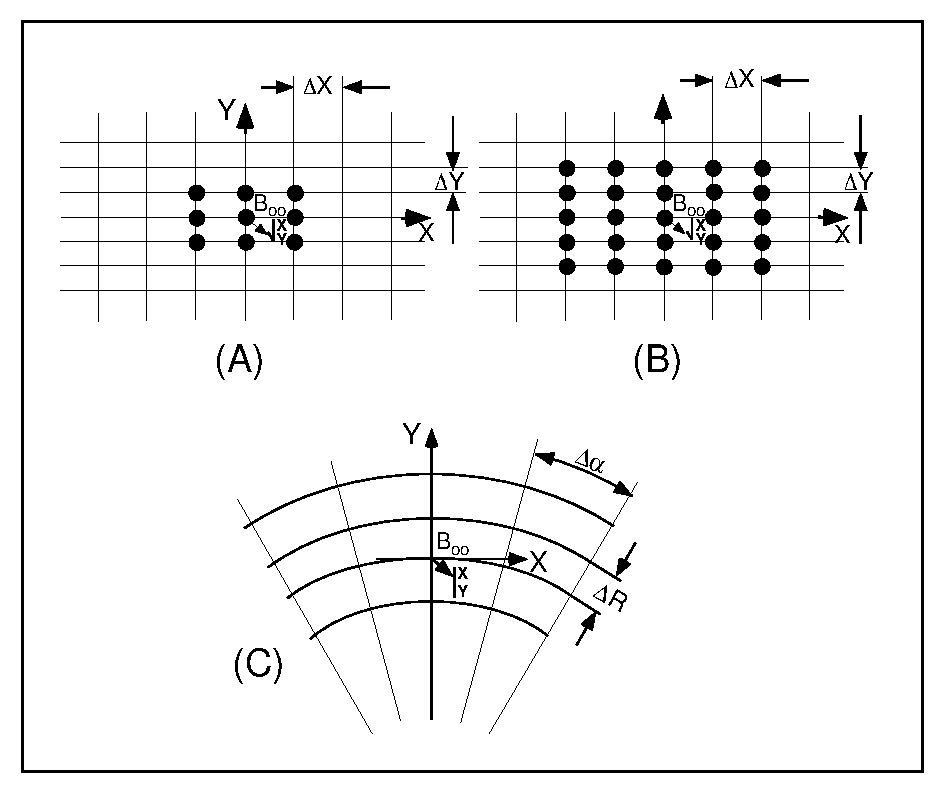
\includegraphics[width=15.5cm]{Fig3.ps}}
\hangcaption[Fig3]{\label{fig3}Mesh in the $ (X,Y) $ plane in Cartesian coordinates.
The grid is centered \\
on the node which is closest to the actual position of the particle.\\
A~: 9-point interpolation  grid.\\
B~: 25-point interpolation grid.\\ 
C~: Mesh in the $ (X,Y) $ plane in polar coordinates. }
	\end{figure}

\subsubsection{Arbitrary 2-D Map, no Symmetry} \label{sec2.4.3}

The map is supposed to describe the field $ \vec  B(B_X,B_Y,B_Z) $
in the $ (X,Y) $ 
plane at elevation $ Z_0 $. It provides the components $ B_{X,ij}$, $
B_{Y,ij}$,  $ B_{Z,ij} $ at 
each node $ (i,j) $ of a 2-D mesh. 

\noindent The value of $ \vec  B $ and its derivatives at the projection $
(X,Y,Z_0) $ of the actual position $ (X,Y,Z) $ 
of a particle is obtained by means of a polynomial interpolation from a  
$3 \times 3$~points grid centered at the node $(i,j) $
which is closest to the position $ (X,Y)$

 \begin{equation}
	 B_{\ell} (X,Y,Z_0)=A_{00} +A_{10} X +A_{01} Y +A_{20} X^2 +A_{11} X Y +A_{02} Y^2
 	\label{eq2-4-10}
 \end{equation}
 %
where $ B_{\ell} $ stands for any of the three components $ B_X$, 
$B_Y $ or $ B_Z $. 
Differentiating then gives the derivatives

\begin{equation}
	\begin{aligned}
		 \dfrac{ \partial B_{\ell} }{ \partial X} \,(X,Y,Z_0)
		     & =   A_{10} +2 A_{20} X + A_{11} Y  \\
		\dfrac{ \partial^2 B_{\ell} }{ \partial X\partial Y}\, (X,Y,Z_0)
		     & =  A_{11} \\
		\text{etc.}
	\end{aligned}
	\label{eq2-4-11}
\end{equation}


\noindent Then follows the procedure of extrapolation from $ (X,Y,Z_0) $ to
the actual position $ (X,Y,Z)$. 

\noindent No special symmetry is assumed, which allows the treatment of 
arbitrary field distribution. 

\noindent Fourth order polynomial interpolation is available upon request (parameter 
\textsl{IORDRE} in  keyword data list - see \textsl{MAP2D,~MAP2D-E}), using 
the method above based on eq.~(\ref{eq2-4-10} developped up to fourth order in $X$ and $Y$. 


\subsubsection{Calculation of $\vec B $ from  3-D Field Map} \label{sec2.4.4}

The vector field $ \vec  B(X,Y,Z) $ and its derivatives necessary
for the calculation of position and velocity of the particle are now defined by means 
of a 3-D field map, through second degree  polynomial interpolation

\begin{equation}
\!\!	B_{\ell} (X,Y,Z) = A_{000} + A_{100} X + A_{010} Y + A_{001} Z + 
	A_{200} X^2 + A_{020} Y^2  
	+     A_{002} Z^2 + A_{110} X Y + A_{101} X Z + A_{011} Y Z
	\label{eq2-4-12}
\end{equation}

\noindent$ B_{\ell} $ stands for any of the three components, $ B_X, $ $ B_Y $
or $ B_Z $.  By 
differentiation of $ B_{\ell} $ one gets 

\begin{equation}
	\begin{aligned}
		 \dfrac{ \partial B_{\ell} }{ \partial X} 
		    & =  A_{100} + 2 A_{200} X + A_{110} Y + A_{101} Z\\
		\dfrac{\partial^2 B_{\ell}}{ \partial X^2} 
		    & =  2 A_{200} 
	\end{aligned}
	\label{eq2-4-13}
\end{equation}
%
 and so on for first and second order derivatives with respect to 
 $X$, $ Y $ or $ Z $. 
 
\noindent The interpolation involves a $ 3  \times   3  \times   3$-point 
parallelipipedic grid (Fig.~\ref{fig4}),   
the origin of which is positioned at the node of the 3-D field map which is 
closest to the actual position of the particle. 
\medskip

\noindent Let $ B^{\ell}_{ijk} $ be the value of the --- measured or computed ---
magnetic field at each one of the 27~nodes of the 3-D grid ($ B^{\ell} $ stands for  
$ B_X$, $ B_Y $ or $ B_Z $), and $ B_{\ell} (X,Y,Z) $ be the value at a
position $ (X,Y,Z) $ 
with respect to the central node of the 3-D grid. Thus, any 
coefficient $ A_i $ of the polynomial expansion of $ B_{\ell} $ is obtained by
means of expressions that minimize, with respect to $ A_i $, the sum
%
\begin{equation}
	S = \sum_{ijk} \left(B_{\ell} (X,Y,Z)-B^{\ell}_{ijk} \right)^2 
	\label{eq2-4-14} %% reel~: 2-4-15
\end{equation}
%
 where the indices $ i$, $j $ and $ k $ take the values -1, 0 or +1 so as
to sweep the 3-D grid. The source code contains the explicit analytical 
expressions of the coefficients $A_{ijk}$ solutions of the normal 
equations $\partial S / \partial A_{ijk} = 0$.


%%%%%%%%%%%%%%figure%%%%%%%%%%%%%%
\begin{figure}[H]
%\vspace{11 truecm}
%%%Figure 4
\centerline{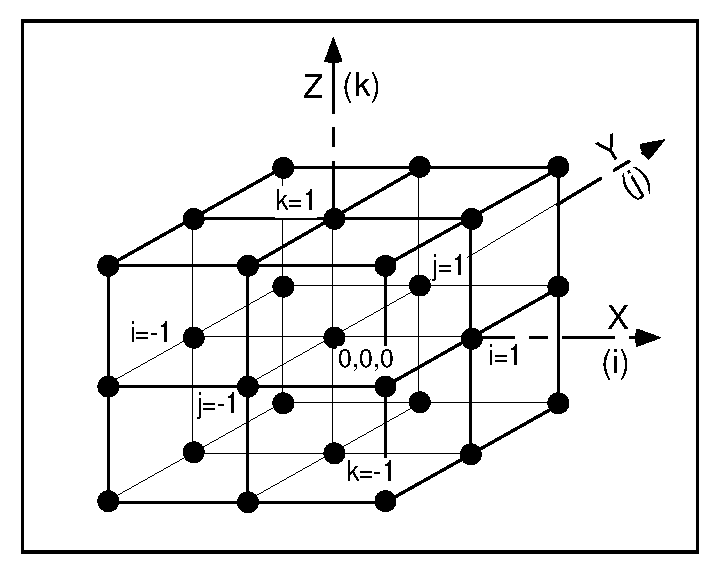
\includegraphics[width=14cm]{Fig4.ps}}
\hangcaption{\label{fig4}A 3-D 27-point  grid is used for
interpolation of $ \vec  B $ and its 
derivatives up to second order.  The central node of the grid $ (i=j=k=0) $ is
at the closest vicinity of the actual position of the particle.} 
\end{figure}

\subsection{Calculation of  $ \vec E $ and its derivatives} \label{sec2.5}

\zgou\ calculates $ \vec  E(X,Y,Z) $ and its derivatives in
 various ways, depending  whether field maps or analytical 
representations of optical elements are used. The  basic 
means are the following~\cite{Biblio6}.     %%% [6]. 

\subsubsection{Extrapolation from  1-D axial field map} \label{sec2.5.1}

 A cylindrically symmetric field can be described by an 
axial 1-D field map of its longitudinal component $ E_X(X,r=0)$ 
$(r=(Y^2+Z^2)^{1/2})$,  
while the radial component $ E_r(X,r=0) $ is assumed to be zero 
(e.g.~in \textsl{ELREVOL\index{ELREVOL}}). $ E_X(X,r=0) $ is obtained at any point along the $ X$-axis by
a polynomial interpolation from the map mesh (see section~\ref{sec2.4.1}). Then the 
field components $ E_X(X,r)$,  $ E_r(X,r) $ at the position of the particle, 
$(X,r) $ are obtained from Taylor expansions to the fifth order in $ r $ (hence, up to 
the fifth order derivative 
$  \dfrac{ \partial^5 E_X }{ \partial X^5}\, (X,0)$),  assuming cylindrical symmetry 
% 
 \begin{equation}
	 \begin{aligned}
		 E_X (X,r)
		   &  =    E_X (X,0) - \dfrac{r^2 }{ 4} \dfrac{\partial^2 E_X }{ \partial X^2} \,(X,0)
		      + \dfrac{r^4 }{64} \dfrac{\partial^4 E_X }{ \partial X^4} \,(X,0)\\
		E_r(X,r)
		   & =   - \dfrac{r }{ 2} \dfrac{\partial E_X }{ \partial X}\, (X,0) 
		     + \dfrac{r^3 }{ 16} \dfrac{\partial^3 E_X }{ \partial X^3} \,(X,0)
		     - \dfrac{r^5 }{ 384} \dfrac{\partial^5 E_X }{ \partial X^5} \,(X,0)
	 \end{aligned}
 	\label{eq2-5-1}
 \end{equation}
\newpage %%%%

\noindent By differentiation with respect to $ X $ and $ r$,  up to the second
order, these expressions provide the derivatives of $ \vec  E(X,r)$.  Finally a conversion
from the $ (X,r) $ coordinates to the $ (X,Y,Z) $ Cartesian coordinates of 
\zgou\ is performed, thus providing the expressions 
$  \dfrac{ \partial^{i+j+k} \vec  E }{ \partial X^i\partial Y^j\partial Z^k} $ 
needed in the eqs.~(\ref{eq2-2-12}). 



\subsubsection{1-D (Axial) Analytical E-Field Models and Extrapolation} \label{sec2.5.2}


This procedure assumes cylindrical symmetry with respect to the $ X$-axis.
 The longitudinal field component $ E_X(X,r=0) $ $ (r=(Y^2+Z^2)^{1/2}) $,
along this axis are derived from differentiation of an adequate 
model of the electrostatic potential $ V(X) $ (e.g.~in \textsl{EL2TUB\index{EL2TUB}, 
UNIPOT\index{UNIPOT}}). 
The longitudinal and radial field components $ E_X(X,r)$,  $ E_r(X,r) $ and 
their derivatives off-axis 
$  \dfrac{ \partial^{i+j}E_X }{ \partial X^i\partial r^j} $ and 
$  \dfrac{ \partial^{ i+j} E_r }{ \partial X^i\partial r^j} $  are obtained by 
Taylor expansions to the fifth order in $ r $ assuming cylindrical 
symmetry (see eq.~(\ref{eq2-5-1})), and then transformed to the $ (X,Y,Z) $ 
Cartesian frame of \zgou\ in order to provide the derivatives 
$ \dfrac{ \partial^{i+j+k} \vec  E }{ \partial X^i\partial Y^j\partial Z^k} $ 
needed in eq.~(\ref{eq2-2-12}).



\subsubsection{2-D Analytical E-Field Models and Extrapolation} 

Several optical elements such as \textsl{WIENFILT\index{WIENFILT}} (that 
uses the \textsl{BEND} fortran routines) 
have their field defined from the  expression of the field and derivatives in the median plane. 
3-D extrapolation of these off the median is drawn from Taylor expansions. 





\subsubsection{3-D Analytical models of fields} \label{sec2.5.3}

 Various electrostatic or magneto-electrostatic  elements, e.g.,   \textsl{ELMULT\index{ELMULT}},
  \textsl{EBMULT\index{EBMULT}}), have their $ \vec  E$ field 
components,  namely $ E_X $, $ E_Y $, $ E_Z $, as well as the 
derivatives with respect to $ X$, $Y $ or $ Z $,  derived 
from  analytical expressions  drawn from  models of the potential $ V(X,Y,Z)$. 





%\vfill\eject

\paragraph{Multipoles And Skewed Multipoles}

\noindent A right electric multipole is considered to have the same effect 
as the equivalent skewed magnetic multipole. Therefore, 
calculation of the right electric or electro-magnetic multipoles 
(\textsl{ELMULT\index{ELMULT}, EBMULT\index{EBMULT}})   uses the 
same eq.~(\ref{eq2-3-5}) together with the rotation process as described in 
section~\ref{sec2.3.5}. The same method is used, for arbitrary rotation of 
arbitrary multipole component around the $ X $-axis. 



\subsection{Calculation Of  $ \vec E$ From Field Maps} \label{sec2.6}

\paragraph{1-D axial map, with cylindrical symmetry} 

\noindent The only type of field map treated in the actual version is the 
1-D axial map, with cylindrical symmetry. The same procedure as 
for the case of magnetic fields is involved (see section~\ref{sec2.4.1}). 


\clearemptydoublepage

\section[SPIN TRACKING]{SPIN TRACKING\index{spin tracking}~\protect\cite{Biblio7}}\label{sec3}   %%% [7]

%%% chgt de numerotation des equations pour ne pas avoir 3.0.1 %%%
%% \renewcommand\theequation{\thesubsection.\arabic{equation}}
\renewcommand\theequation{\thesection.\arabic{equation}}
\makeatletter
\@addtoreset{equation}{section}
\makeatother
%%%

The depolarization of a particle beam travelling in a 
magnetic field $ \vec  b $ takes its origin in the spin  
precession undergone by each particle. This motion of the spin $ \vec  S $ 
is governed by the Thomas-BMT first order differential equation~\cite{Biblio8}       %%%%[8] 


\begin{gather}
	\dfrac{d\vec  S }{ dt} = \dfrac{q }{  m} \, \vec  S\times\vec  \Omega
	     \label{eq3-1}  \\
\intertext{where}
	\vec  \Omega  = (1+\gamma G)\vec  b + G(1-\gamma )\vec  b_{\paral} \label{eq3-2} 
\end{gather}

\noindent$ q$, $m$, $\gamma$ and $ G $ are respectively the charge, 
mass, Lorentz relativistic factor, and anomalous magnetic moment of the 
particle. $ \vec  b_{\paral} $ is the component of $ \vec  b $ which is
parallel to the velocity $ \vec  v $ of the particle. 

\noindent These equations are normalized by introducing the same notation 
as previously. Let $ b=\parallel\vec  b\parallel $ and $ v=\parallel\vec v\parallel$~;  
$ ds=vdt $ is the differential path, $ \dfrac{\gamma mv }{ q} = \Br $ is the
rigidity of the particle~; 
$ \vec  S^{\,\prime} = \dfrac{d\vec  S }{ ds} = \dfrac{1 }{ v}\dfrac{d\vec  S }{ dt} $ 
is the derivative of the spin with respect to the path. 

\noindent Introducing also $ \vec  B= \dfrac{\vec  b }{ \Br} $, 
$ \vec B_{\paral} = \dfrac{\vec  b_{\paral} }{ \Br} $  and

\begin{equation}
	\vec  \omega  = \frac{\vec \Omega }{ \Br}  = (1+\gamma G)\vec  B +
	G(1-\gamma )\vec  B_{\paral}
	\label{eq3-3}
\end{equation}
%
eq.~(\ref{eq3-1}) can be re-written in a normalized way

 \begin{equation}
	 \vec  S^{\,\prime}  = \vec  S \times  \vec  \omega
 	\label{eq3-4}
 \end{equation}
 
\noindent This equation is then solved in the same way as the reduced Lorentz 
equation~(\ref{eq2-2-3}). 
From the values of the magnetic factor $ \vec  \omega (M_0) $ and the spin 
$\vec  S(M_0) $ 
of the particle at position $ M_0 $ of its trajectory, the spin $ \vec  S(M_1)$ 
at position $ M_1 $, following a displacement $ \Delta s$ (fig. 2), is obtained from truncated 
Taylor expansion 

 \begin{equation}
	 \vec  S(M_1) \approx \vec  S(M_0)+ \dfrac{d\vec  S }{ ds} (M_0)\, \Delta s
	 + \dfrac{d^2\vec  S }{ds^2} \,(M_0) \dfrac{\Delta s^2 }{ 2} 
	 + \dfrac{d^3\vec  S }{ ds^3} \,(M_0) \dfrac{\Delta s^3 }{ 3!}
	+ \dfrac{d^4\vec  S }{ ds^4}\, (M_0) \dfrac{\Delta s^4 }{ 4!}
 	\label{eq3-5}
 \end{equation}
 
\noindent The derivatives $ \vec  S^{(n)} = \dfrac{d^n\vec  S }{ ds^n} $ of 
$\vec  S $ at $ M_0 $ are obtained by differentiating eq.~(\ref{eq3-4})

 \begin{equation}
	 \begin{aligned}
		 \vec  S^{\,\prime}  
		      &  =\vec  S\times\vec  \omega \\
		\vec  S^{\,\prime\prime} 
		      &  =\vec  S^{\,\prime} \times\vec  \omega +\vec  S\times\vec  \omega ^\prime \\
		\vec  S^{\,\prime\prime\prime}
		      &  =\vec  S^{\,\prime\prime} \times\vec  \omega +2\vec  S^{\,\prime} \times\vec  \omega ^\prime 
		           +\vec S\times\vec  \omega^{\prime\prime} \\
		\vec  S^{\quaprime} 
		      & =\vec S^{\,\prime\prime\prime} \times\vec  \omega 
		          +3\vec  S^{\,\prime\prime} \times\vec \omega^\prime 
		          +3\vec  S^{\,\prime} \times\vec  \omega^{\prime\prime} 
		          +\vec S\times\vec  \omega^{\prime\prime\prime}
	 \end{aligned}
 	\label{eq3-6}
 \end{equation}
 %
  where the derivatives $ \vec  \omega^{(n)} $ are obtained from eq.~(\ref{eq3-3}). 
  
\noindent The last point consists in getting $ \vec  B_{\paral} $ and its
derivatives. 
This can be done in the following way. 
Let $ \vec  u=\dfrac{\vec  v }{ v} $ be the normalized velocity of the particle,
then,

\begin{equation}
	\begin{aligned}
		\vec  B_{\paral} 
		     & = (\vec  B \cdot\vec  u)\, \vec  u \\
		\vec  B^{\,\prime}_{\paral}  
		     & = (\vec B^{\,\prime} \cdot\vec  u+\vec  B\cdot\vec  u^{\,\prime} )\,\vec  u
		       +(\vec  B\cdot\vec  u)\,\vec u^{\,\prime} \\
		\vec B^{\,\prime\prime}_{\paral}  
		     & = (\vec  B^{\,\prime\prime} \cdot\vec  u+2\vec B^{\,\prime} \cdot\vec  u^{\,\prime} 
		       +\vec  B\cdot\vec  u^{\,\prime\prime} )\, \vec  u
		       +2(\vec B^{\,\prime} \cdot\vec  u+\vec  B\cdot\vec  u^{\,\prime} )\,\vec  u^{\,\prime} 
		       +(\vec  B\cdot\vec u)\,\vec  u^{\,\prime\prime}\\
		\text{etc.}
	\end{aligned}
	\label{eq3-7}
\end{equation}


\noindent The quantities $ \vec  u$,  $ \vec  B $ and their n-th derivatives
as involved in these equations are picked up from eqs.~(\ref{eq2-2-6}, \ref{eq2-2-7}).



\clearemptydoublepage

\section{SYNCHROTRON RADIATION }\label{secN4}\index{synchrotron radiation} 

%%% on a de nouveau une numerotation des equations 4.1.1 %%%
\renewcommand\theequation{\thesubsection.\arabic{equation}}
\makeatletter
\@addtoreset{equation}{subsection}
\makeatother

\zgoubi\ allows the simulation of two types of synchrotron radiation (SR) related effects 
 namely, on the one hand 
energy loss by stochastic emission of photon and the ensuing perturbation 
on particle dynamics  and, on the other hand calculation of the 
radiated spectral-angular energy densities as observed in the lab. 

\subsection{Energy loss and related dynamical effects~\protect\cite{FMSEA-00-01}}\label{secSRLoss}

Given a particle wandering in the magnetic field of an arbitrary optical element or field 
map, \zgoubi\ computes the energy loss undergone, and its 
effect on the particle motion. The energy loss is calculated  in a  classical manner, by calling upon 
two random processes that accompany the emission of a photon  namely, \\
\indent - the probability of emission, \\
\indent - the energy of the photon. 

The effects on the dynamic of the emitting particle 
 is either limited to the alteration of the energy, or extended to angular kick effect, 
following user requested working options~; particle 
position is supposed not to  change upon emission of a photon. These calculations 
 and ensuing dynamics corrections are performed after 
 each integration step. In a practical manner, this 
means every centimer or tens of centimers in smoothly varying magnetic fields. 

Main aspects of the method are developped in the following. 

\paragraph{Probability of emission of a photon}

Given that the number of photons emitted within a step $\Delta s$ can be very low (units or fractions 
of unit)\footnote{For instance, a $1\,$GeV electron will emit about $20.6$ photons per radian~; an 
 integration step size $\Delta s =0.1\,$m upon $\rho=10\,$m bending radius results in 0.2 photons 
per step.} a Poisson probability law 
\begin{equation}
	\label{EqPoiss}
 p(k) = \frac{\lambda^{-k}}{k!} exp(-k)
\end{equation}
is considered. $k$ is the number of photons emitted over a $\Delta \theta$ (circular) arc of 
trajectory  such that, the mean number of photons per radian expresses as\footnote{This leads for 
instance, in the case of electrons, to the classical formula $\lambda/\Delta \theta \approx
129.5$E(GeV)$/2\pi\approx \gamma/94.9$.}
\begin{equation}
        \label{EqPoissMean}
 \lambda = \frac{20 e r_0 }{8 \bar{h} \sqrt{3}  } \beta^2 \Br  \Delta s
\end{equation}
where $r_0=e^2/4\pi \epsilon_0 m_0 c^2$ is the classical radius of the particle of rest-mass $m_0$, 
$e$ is the elementary 
charge, $\bar{h} = h/2\pi , h$ is the Planck constant, $\beta = v/c$, $\Br$ is the particle 
stiffness. $\lambda$ is evaluated at each integration step from the current values $\beta$, $\Br$ 
and $\Delta s$,  then a value of $k$ is drawn by a rejection method~\cite[routine POIDEV]{NumRec}.  


\paragraph{Energy of the photons}

These k photons are assigned energies $\epsilon=h\nu$ at random, in the following way. The cumulative 
distribution of the energy probability law $p(\epsilon/\epsilon_c)d\epsilon/\epsilon_c$  writes 
\begin{equation}
\label{EqSK53}
\mathcal{P}(\epsilon/\epsilon_c) = \frac{3}{5\pi} \int_0^{\epsilon/\epsilon_c} 
\int_{\epsilon/\epsilon_c}^\infty K_{5/3}(x) dx
\end{equation}
where $K_5/3$ is a modified Bessel function and, $\epsilon_c= \bar{h} \omega_c$
with $\omega_c=2 \pi 3 \gamma^3 c / 2 \rho$ being the critical frequency  of the radiation in 
constant field with bending radius $\rho$~;  $\omega_c$ is evaluated at each integration step from 
the current values $\gamma$ and $\rho$, in other words, this energy loss calculation 
assumes constant  magnetic field~\footnote{From 
a practical viewpoint, note that the value of the magnetic field first computed for a 
one-step push of the particle  (eqs.~\ref{eq2-2-4},\ref{eq2-2-6}) is next used to  obtain  
$\rho$ and perform SR loss corrections afterwards.}  over the trajectory arc $\Delta s$. 
In the low frequency region $(\epsilon/\epsilon_c \ll 1)$ it can be approximated by 
\begin{equation}
\label{EqSK53Low}
\mathcal{P}(\epsilon/\epsilon_c) = \frac{12 \sqrt{3}}{5\, 2^{1/3} \Gamma(\frac{1}{3})}  
(\frac{\epsilon}{\epsilon_c})^{1/3}
\end{equation}


\begin{wrapfigure}{r}{8cm}

\vspace{5mm}  \centerline{\includegraphics[width=6cm]{G.eps}}

\vspace{4mm}
  \begin{center} 
 {\footnotesize 
       Cumulative distribution   $\mathcal{P}(\epsilon/\epsilon_c)$. }
  \end{center} 

\vspace{-6mm}
\end{wrapfigure}

 About $40$ values of $\mathcal{P}(\epsilon/\epsilon_c)$ computed from eq.~\ref{EqSK53}~\cite{VOKostroun}, 
honnestly spread  over a range $\epsilon/\epsilon_c \leq 10$ are  tabulated 
in \zgoubi\ source file (see figure). In 
order to get $\epsilon/\epsilon_c$, first a random value $0<\mathcal{P}<1$ is generated uniformly, 
then  $\epsilon/\epsilon_c$ is drawn either  by simple inverse linear interpolation 
 of the tabulated values if $\mathcal{P}>0.26$ (corresponding to 
$\epsilon/\epsilon_c>10^{-2}$), 
or, if $\mathcal{P}<0.26$ from eq.~\ref{EqSK53Low} that directly gives 
 $\epsilon/\epsilon_c= \bigl( \frac{5 \, 2^{1/3} \Gamma(\frac{1}{3})}{12 \sqrt{3} \mathcal{P}}\bigr)^3$ 
 with precision no less than 1$\%$ at  $\mathcal{P}\rightarrow 0.26$. 

\bigskip


Upon request of SR loss tracking, several optical elements that contain dipole 
magnetic field component (e.g., \textsl{MULTIPOL}) provide a printouot of various 
 quantities related to SR emission, as drawn from classical theoretical 
expressions, such as for instance, \\
- energy loss per particle $\Delta E(eV)= \frac{2}{3}r_0 c \gamma^3 B(T) \Delta \theta$,   ($B$ 
is the dipole field, exclusive of any other multipole component or non-linearity 
in the magnet~; $\Delta \theta$ is the total deviation as calculated from $B$, the 
magnet length, and the reference rigidity \BORO (as defined with, e.g., \textsl{OBJET}) \\
- energy $\epsilon_c(eV)=\frac{3 \gamma^3 c}{2 \rho} \frac{\bar{h}}{e}$, with 
$\rho =$\BORO$/B$ \\
- energy of radiated photons $<\epsilon> = \frac{8}{15 \sqrt{3}} \epsilon_c$, \\ 
- r.m.s. energy of radiated photons $\epsilon_{rms} = 0.5591 \epsilon_c$, \\
- number of radiated photons per particle  $N = \Delta E /<\epsilon>$.  

This is done in order to facilitate verifications, since on the other hand statistics 
regarding those values are drawn from the tracking and printed upon use of the dedicated 
keyword \textsl{SYNPRNL}. 



\bigskip

Finally, upon user's request as well,  SR loss can be limited to particular classes of optical 
elements, for instance dipole fields alone, or dipole + quadrupole magnets, etc. These tricks 
are made available in order to permit deeper insight, or easier comparison with other codes, 
for instance. 

\subsection{Spectral-angular radiated densities~\protect\cite{FMSL/94-22,FMLPYellow}}\label{secSRSpec}


The ray-tracing procedures provide the ingredients necessary 
for the determination of the electric field radiated by the particle subject to
acceleration, as shown in Fig.~\ref{newfig5} (section~\ref{secN4.1}). This allows 
calculation\footnote{These procedures are for the moment  implemented in the 
post-processor  \textbf{zpop} \index{zpop}}   
of spectral-angular densities radiated by particles in magnetic fields (section~\ref{secN4.2}). 


%%%%%%%%%%%%%%figure%%%%%%%%%%%%%%
%\vspace{1cm}
\begin{figure}  %[H]
%\vspace{4.5 truecm}
%%%Figure 6
\centering
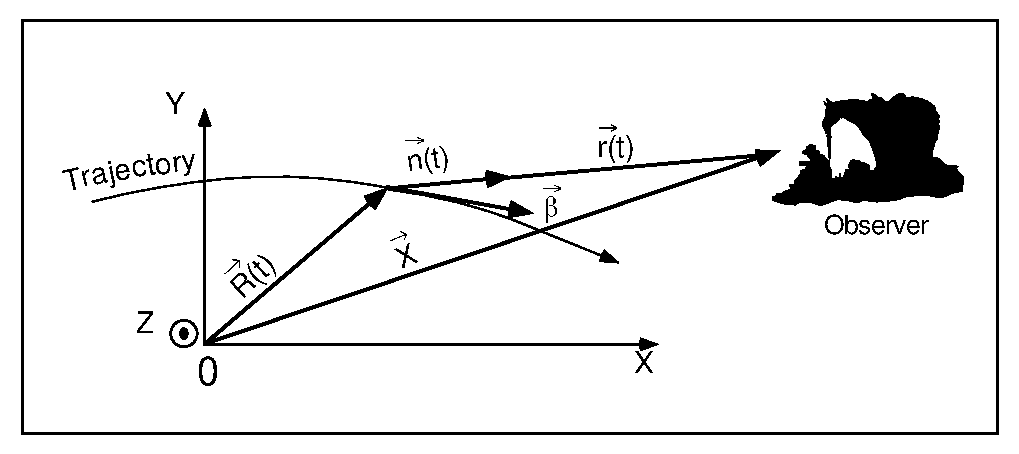
\includegraphics[width=16cm]{NewFig5.ps} 
{\setlength{\captionwidth}{15cm}
\hangcaption[NewFig 6]{\label{newfig5}A scheme of the reference frame in 
\zgou\ together with the vectors entering
in the definition of the electric field radiated by the accelerated particle~:\\
$(x,y)$~: horizontal plane~;~$z$~: vertical axis.\\
$\vec{R}(t)$ = particle position in the fixed frame $(O, x, y, z)$~;\\
$\vec{X}$ (time-independent) = position of the observer in the  $(O, x, y, z)$ frame~;\\
$\vec{r}(t) = \vec{X} - \vec{R}(t)$ = position of the particle with respect to
the observer~;\\
$\vec{n}(t)$ = (normalized) direction of observation = $\vec{r}(t)/|\vec{r}(t)|$~;\\
 $\vec{\beta}$ = normalized velocity vector of the particle $\vec{v}/c = 
 (1/c) d\vec{R}/dt$.} }
\end{figure}
%

%\subsubsection{Calculation of the radiated 
% electric field $\vec \Ecal (\vec n, \tau)$  \label{secN4.1}}
\subsubsection{Calculation of the radiated  electric field  \label{secN4.1}}


The expression for  the radiated  electric field $\vec \Ecal (\vec{n}, \tau)$ 
as seen by the observer in the long
distance approximation is~\cite{JDJ}
\begin{equation}
\vec \Ecal (\vec{n}, \tau) = 
	\frac{q}{4\pi\varepsilon_0c}\, 
	\frac{\vec{n}(t) \times \left[
		\left(\vec{n}(t)- \vec{\beta}(t) \right) 
		\times d\vec{\beta}/dt \right]}%
	{r(t) \left(1 - \vec{n}(t)\cdot\vec{\beta}(t) \right)^3}
 \label{eqN4.1}
\end{equation}
%\end{equation} \label{eqN4.1}
%
where $t$ is the time in which the particle motion is described and $\tau$ is the
observer time. Namely, when at position $\vec{r}(t)$ with respect to the observer [or as
well at position $\vec{R}(t) = \vec{X} - \vec{r}(t)$ in the ($O, x, y, z$) frame] the
particle emits a signal which reaches the observer at time $\tau$, such that $\tau = t +
r(t)/c$ where  $r(t)/c$ is the delay necessary for the signal to travel from the
emission point to the observer, which also leads by differentiation to the well-known
 relation

\begin{equation}
d\tau/dt = 1 - \vec{n}(t) \cdot \vec{\beta}(t)  \label{eqN4.2}
\end{equation} 
%\end{equation} \label{eqN4.2}

\noindent The vectors $\vec{R}(t)$ and $\vec{\beta}(t) = \frac{v}{c} \vec u$ (eq.~\ref{eq2-2-2}) that describe the motion are obtained from the ray-tracing (eqs.~\ref{eq2-2-4}). The acceleration is calculated  from~(eq.~\ref{eq2-2-1})
\begin{equation}
d\vec{\beta}/dt = (q/m)~\vec{\beta}(t) \times \vec{b}(t) \label{eqN4.3}
\end{equation} %\label{eqN4.3}

\noindent Then, given the observer position $\vec{X}$ in the fixed frame, it is possible
to calculate
\begin{equation}
\vec{r}(t) = \vec{X} - R(t) \text{ and } \vec{n}(t) = \vec{r}(t)/ |\vec{r}(t)| \label{eqN4.4}
\end{equation} %\label{eqN4.4}

\section*{The calculation of $\vec{n} - \vec{\beta}$ and $1 - \vec{n} \cdot \vec{\beta}$}
 
Owing to computer precision the crude computation of $\vec{n} -
\vec{\beta}$ and $ 1 -\vec{n}\cdot \vec{\beta}$ may lead to
$$
	\vec{n} - \vec{\beta} = 0 \text{ and } 1 - \vec{n}\cdot \vec{\beta} = 0
$$
since the preferred direction of observation is generally almost parallel to
$\vec{\beta}$ (exactly parallel in the sense of computer precision), while $\beta
\approx$ 1 as soon as particle energies of a few hundred times the rest mass are
concerned.

\noindent It is therefore necessary to express $\vec{n} - \vec{\beta}$ 
and $1 -\vec{n} \cdot
\vec{\beta}$ in an adequate  form for achieving accurate software  computation.

\noindent The expression for $\vec{n}$ is

\begin{multline} \label{eqN4.5}
	\vec{n} = (n_x, n_y, n_z) = (\cos \psi\,\cos \phi, \cos \psi \,\sin 
		\phi, \sin \psi)  \\
	= \left[1 - 2 (\sin^2\phi/2 + \sin^2 \psi/2) + 4 \sin^2\phi/2 \sin^2\psi/2, 
		\sin \phi (1 - 2\sin^2\psi/2), \sin \psi \right]
\end{multline}
%
where $\phi$ and $\psi$ are the observation angles, given by 

\begin{equation}
	\phi = \text{Atg} \left( \frac{r_y}{ r_x}\right)
	\text{ and }  \psi = \text{Atg}\left( \frac{r_z}{\sqrt{r_x^2 + r_y^2}}\right) \label{eqN4.6}
\end{equation} %\label{eqN4.6}
%
with $\vec{r} = (r_x, r_y, r_z)$, while $\vec{\beta}$ can be written under the form

\begin{multline} \label{eqN4.7}
	\vec{\beta} = (\beta_x, \beta_y, \beta_z) = 
		\left[ \sqrt{(\beta^2 - \beta^2_y - \beta_z^2)},\beta_y, \beta_z 
		\right] \\
	= \left[ \sqrt{(1 - 1/\gamma^2 - \beta_y^2 - \beta_z^2)}, \beta_y, 
		\beta_z \right] = (1 - a/2 + a^2/8 - a^3/16 +...,\beta_y, \beta_z) 
\end{multline}
%
where $a = 1/ \gamma^2 + \beta^2_y + \beta^2_z$. This leads to

\begin{gather*}
	n_x = 1 - \varepsilon_x 
		\text{ and } \beta_x = 1 - \xi_x  \\
\intertext{with}
\varepsilon_x = 2 (\sin^2\phi/2 + \sin^2\psi/2) - 4 \sin^2\phi/2  \sin^2\psi/2 \\
\intertext{and}
\xi_x = a/2 - a^2/8 + a^3/16 +...
\end{gather*}

\noindent All this provides, on the one hand, 

\begin{equation}
\vec{n} - \vec{\beta} = (-\varepsilon_x + \xi_x, n_y - \beta_y, n_z - \beta_z)~,  \label{eqN4.8}
\end{equation}   %\label{eqN4.8}
%
whose components are combinations of terms of the same order of magnitude
($\varepsilon_x$ and $\xi_x \sim 1/\gamma^2$ while $n_y, \beta_y, n_z$ and $\beta_z \sim
1/\gamma$) and, on the other hand,

\begin{equation}
1 - \vec{n} \cdot \vec{\beta} = \varepsilon_x + \xi_x - n_y\beta_y - n_z\beta_z -  \label{eqN4.9}
\varepsilon_x\xi_x~,
\end{equation}  %\label{eqN4.9}
%
that combines terms of the same order of magnitude ($\varepsilon_x, \xi_x, n_y\beta_y$
and $n_z\beta_z \sim 1/\gamma^2$), plus $\varepsilon_x\beta_x \sim 1/\gamma^4$.

\noindent The precision of these expressions is
directly related to the order at which the series

$$
	\xi_x = a/2 - a^2/8 + a^3/16 +... \qquad(a = 1/\gamma^2 + \beta_y^2 +\beta^2_z)
	$$
is pushed, however the convergence is   fast since $ a \sim 1/\gamma^2 \ll 1$.

\subsubsection{Calculation of the Fourier transform of the electric field}\label{secN4.2}

The Fourier transforms
$$
	FT_\omega  [ \vec \Ecal (\tau)] = \int \vec \Ecal  (\tau) e^{-i\omega\tau} d\tau~$$
of the $\sigma$ and $\pi$ electric field components provide the spectral angular
 energy density 
\begin{equation}
	\partial^3 W/\partial\phi\, \partial\psi\, \partial\omega 
		= 2 r^2 \left| FT_\omega \left(\vec  \Ecal (\tau) \right)  \label{eqN4.10}
		\right|^2 / \mu_0 c
\end{equation}  %\label{eqN4.10}
%
They are calculated in a regular way, without use of FFT technics, namely from 

\begin{equation}
	FT_\omega \left[ \vec \Ecal  (\tau) \right] 
		\approx \sum \vec \Ecal (\tau_k)\, e^{-i\omega\tau_k} \, \Delta\tau_k  \label{eqN4.11}
\end{equation}    %\label{eqN4.11}
%
for two reasons. On the one hand, the number of integration steps $\Delta s$ that define the
trajectory (eqs.~\ref{eq2-2-4}), is arbitrary and therefore in general not of order $2^n$.
On the other hand, the integration step defines a constant time differential element 
$\Delta t_k = \Delta s/ \beta c$ which results in the observer differential time 
element $ \Delta \tau_k$, which is
also the differential element of the Fourier transform, being non-constant, since both
are related by eq.~\ref{eqN4.2} in which $\vec{\beta}$ and $\vec{n}$ 
vary as a function of the  integration step number $k$.

\noindent Another major point is that  $ \Delta \tau_k$ may reach drastically small values 
in the region of the central peak of the electric impulse emitted in 
a dipole ($1 - \vec{n}(t) \cdot \vec{\beta} (t) \to
1/2\gamma^2$), whereas the total integrated time $\sum_{k=1}^{N} \Delta \tau_k$ may be several
orders of magnitude larger. In terms of the physical phenomenon, the total duration of the electric 
field impulse as seen by the observer corresponds to the time delay $ \sum_{k=1}^{N} \Delta \tau_k$
that separates photons emitted at the
entrance of the magnet from photons emitted at the exit, but the significant  part of it
(in terms of energy density) which can be represented by the width 
$ 2\, \tau_c = \dfrac{2(1 +\gamma^2\psi^2)^{3/2}~2\rho }{ 3\gamma^3~c}$ of the  
radiation peak~\cite{after}, is a very small fraction of $ \sum_{k=1}^{N} \Delta \tau_k$.

\noindent The consequence is that, once again in relation with computer precision, the
differential  element $\Delta \tau_k$ involved in the computation of 
eq.~\ref{eqN4.11} cannot be derived from such relation as 
 $\Delta\tau_k = \sum_{k=1}^{n} \Delta\tau_k - \sum_{k=1}^{n-1} \Delta \tau_k$ 
but instead must be stored as such beforehand in the couorse of the ray-tracing process. 


%%%%%%%%%%%%%%%%% previous part 4 %%%%%%%%%%%%%%%%%%%%%%%%%
\clearemptydoublepage

\section{DESCRIPTION OF THE AVAILABLE PROCEDURES} \label{sec4}

\subsection{Introduction} \label{4.1} 


This chapter gives a detailed description of how the \zgou\ 
procedures work, and their associated keywords. It has been 
split into several sections. Sections~\ref{sec4.2} to~\ref{sec4.5} explain the 
underlying content and functioning of all available keywords. 
Section~\ref{sec4.6} is dedicated to the description of some general 
procedures that may be accessed by means of special data or flags 
(such as negative integration steps), or through the available 
keywords (such as multiturn\index{multiturn} tracking with \textsl{REBELOTE\index{REBELOTE}}). 

\subsection{Definition of an Object} \label{sec4.2}

The description of the object, \emph{i.e.}, initial coordinates of the 
beam, must be the first element of the input data to \zgou. 
 \bigskip

\noindent Several types of automatically generated objects are available, 
as described in the following pages.

\newpage

\subsubsection*{MCOBJET~:  \MCOBJETTitl} \label{MCOBJET} \index{MCOBJET}
\index{Monte Carlo}\index{negative charge}\index{negative momentum}

\noindent \textsl{MCOBJET} generates a set of up to \imax\ random 6-D initial
conditions. It can be used in conjunction with the keyword \textsl{REBELOTE\index{REBELOTE}},
which  moreover allows generating an arbitrarily high number of initial conditions. 
 \bigskip

\noindent The first datum is the reference rigidity (negative value 
allowed)
$$ BORO = \dfrac{p_0 }{ q} \text{ (kG.cm)} $$\index{BORO@{\BORO}}

\noindent Depending on the value of the next datum, \textsl{KOBJ}, the 
\IMAX\index{IMAX@{\IMAX}|textbf} ($\leq \imax$) particles have their initial random 
conditions $ Y$, $T$, $Z$, $P$, $X$ and $ D $ (relative momentum)  generated 
on 3~different types of supports, as described below. 

\noindent Next come the data
$$KY, KT, KZ, KP, KX$$  %%%%%%%%% $$ KH,\quad KV,\quad KP $$
that specify the type of probability density for the 6~coordinates. 

\noindent $KY$, $KT$, $KZ$, $KP$, $KX$ can take the following values~:
\begin{enumerate}
\item uniform density, $p(x) =1/2\delta x$ if  $-\delta x \leq x \leq \delta x$, $p(x) = 0$ elsewhere,
\item Gaussian density, $p(x) = \dfrac{1}{\delta x \sqrt{2\pi}} 
	e^{- \frac{x^2}{2 \delta x^2}}$,
\item parabolic density, $p(x) = \dfrac{3}{4 \delta x} 
	(1- \dfrac{x^2}{\delta x^2})$ if $-\delta x \leq x \leq \delta x$, $p(x) = 0$ elsewhere.
\end{enumerate}

\noindent $KD$ can take the following values~:
\begin{enumerate}
\item uniform density, $p(D) =1/2\delta \! D$ if  $-\delta \! D \leq D \leq \delta \! D$, $p(D) = 0$ elsewhere,
\item exponential density, $p(D) = N_0 \exp (C_0 + C_1 l + C_2 l^2 + C_3 l^3)$
	with $0 \leq l \leq 1$ and $-\delta D \leq D \leq \delta D$,
\item $p(D)$ is determined by a kinematic relation, namely, with $T=$ 
horizontal angle, $D= \delta D \ast T$.
\end{enumerate}

\noindent Next come the central value for the random sorting, 
$$    Y_0,\quad    T_0,\quad    Z_0,\quad P_0,\quad  X_0, \quad D_0 $$
%
namely, the probability density laws $p(x)$ ($x= Y, T, Z, P$ or $X$) 
and $p(D)$ described above apply to the variables $x-x_0$
( $\equiv Y- Y_0$, $T-T_0$, ...) and $D- D_0$ respectively. Negative 
value for $D_0$ is allowed (see section~\ref{sec4.6.7}).
 \bigskip

\noindent\textbf{KOBJ  =  1}~: Random  generation of \IMAX\ particles  
in a hyper-window with widths
(namely the half-extent for uniform or parabolic distributions ($KY, 
KT, ... =1$ or 3), and  the r.m.s.~width for Gaussian distributions ($KY, 
KT, ... =2$))
$$   \delta Y,\quad   \delta T,\quad   \delta Z,\quad   \delta P,\quad   \delta X,\quad  \delta D $$

\noindent Then follow the cut-off values, in units of the 
r.m.s.~widths $\delta Y$, $\delta T$, ... (used only for  Gaussian distributions,  
$KY, KT, ... =2$)
$$
	N_{\delta Y},\quad N_{\delta T},\quad N_{\delta Z},\quad N_{\delta P},\quad N_{\delta X},\quad N_{\delta D}
$$	 
\noindent The last data are the parameters 

$$ N_0,\quad C_0,\quad C_1,\quad C_2,\quad C_3 $$ 
%
 needed for generation of the $ D $ coordinate upon option
 $ KD  =  2$ (unused if $ KD = 1,~3$) and a set of three integer seeds for initialization of random sequences,
 
 $$ IR1,\quad   IR2, \quad  IR3 \quad \text{(all $\simeq 10^6 $)}$$
%

\medskip

\noindent All particles generated by \textsl{MCOBJET\index{MCOBJET}}  are tagged with
a (non-S) character, for further statistic purposes 
(e.g., with \textsl{HISTO\index{HISTO}} and \textsl{MCDESINT\index{MCDESINT}}).  
\medskip

\noindent\textbf{KOBJ  =  2}~: Random  generation of 
$ IY \ast   IT  \ast IZ \ast  IP  \ast  IX  \ast  ID $ particles    
(maximum \imax) in a  hyper-grid.  The input data are the number of bars    in 
each coordinate

 \begin{gather*}
	 IY,\quad IT,\quad IZ,\quad IP,\quad IX, \quad ID \\
%
\intertext{the spacing of the bars} 
	PY,\quad PT,\quad PZ,\quad PP,\quad PX, \quad PD \\
%
\intertext{the width of each bar} 
	\delta Y,\quad \delta T,\quad \delta Z,\quad \delta P,\quad \delta X,\quad \delta D  \\
%
\intertext{the cut-offs, used with Gaussian densities (in units of the r.m.s. widths)}
	N_{\delta Y},\quad N_{\delta T},\quad N_{\delta Z},\quad N_{\delta P},\quad N_{\delta X},\quad N_{\delta D}
 \end{gather*}
%\medskip

\noindent This is illustrated in Fig.~\ref{fig5}.

\medskip

\noindent The last two sets of data in this option are the parameters 

 \begin{gather*}
	N_0,\quad C_0,\quad C_1,\quad C_2,\quad C_3 
 \end{gather*}
%
 needed for generation of the $ D $ coordinate upon option \mbox{KD=  2}  
(unused if \mbox{KD= 1, 3}) and a set of three integer seeds for initialization 
of random sequences, $ IR1$,   $ IR2$,   and $ IR3$ (all $\simeq 10^6 $).

%\medskip

\noindent All particles generated by \textsl{MCOBJET\index{MCOBJET}}  are tagged with
a (non-S) character, for further statistic purposes (see \textsl{HISTO\index{HISTO} \textrm{and}  
MCDESINT\index{MCDESINT}}).  

\medskip

\noindent\textbf{KOBJ  = 3~:} Distribution of \IMAX\ particles inside a
6-D ellipsoid defined by the three sets of data (one set per 
 2-D phase-space)

$$
\begin{array}{*{4}{r<{,}}r}
 \alpha_ Y  &   \beta_ Y  
            &  \dfrac{ \varepsilon_Y}{\pi} 
            &  N_{\varepsilon_ Y}  ~~[
            & N'_{\varepsilon_ Y}, \text{ if } N_{\varepsilon_ Y} < 0] \\
\alpha_ Z   &  \beta_ Z  
            &  \dfrac{ \varepsilon_Z }{ \pi} 
            & N_{\varepsilon_ Z} ~~[
            & N'_{\varepsilon_ Z}, \text{ if } N_{\varepsilon_ Z} < 0] \\
\alpha_ X   & \beta_ X 
            &  \dfrac{\varepsilon_X }{ \pi} 
            & N_{\varepsilon_ X} ~~[
            & N'_{\varepsilon_ X}, \text{ if } N_{\varepsilon_ X} < 0] 
\end{array}           
$$            
%
where $\alpha$, $\beta$ are the ellipse parameters and $\varepsilon/ 
\pi$ the emittance, corresponding to an elliptical  frontier 
$\dfrac{1 + \alpha^2_Y}{\beta_Y} Y^2 + 2 \alpha_Y YT + \beta_Y T^2 = 
\varepsilon_Y / \pi$ (idem for the ($Z, P$) 
or ($X, D$) planes). $N_{\varepsilon_ Y}$, $N_{\varepsilon_ Z}$ and 
$N_{\varepsilon_ X}$ are the sorting cut-offs (used only for Gaussian 
distributions, $KY, KT, ...=2$).

\noindent The sorting is uniform in surface (for $KY=1$, or $KZ=1$ 
or $KX=1$) or Gaussian ($KY=2$ or $KZ=2$), and so on, as described 
above. A uniform sorting has the ellipse above for support. A 
Gaussian sorting has the ellipse above for r.m.s.~frontier, leading 
to $\sigma_Y = \sqrt {\beta_Y \varepsilon_Y / \pi}$, 
$\sigma_T = \sqrt {\dfrac{(1+\alpha_Y^2)}{\beta_Y} \varepsilon_Y / \pi}$, 
and similar relations for $\sigma_Z$, $\sigma_X$.

\noindent If $N_\varepsilon$ is negative, thus the sorting fills the 
elliptical ring that extends from $\left| N_\varepsilon \right|$ to 
$N'_\varepsilon$ (rather than the inner region determined by the $N_\varepsilon$ 
cut-off, as addressed above).
\newpage
\vfill
%%%%%%%%%%%%%%figure %%%%%%%%%%%%%
 \begin{figure}[H]
  % \vspace*{19 truecm}
\centerline{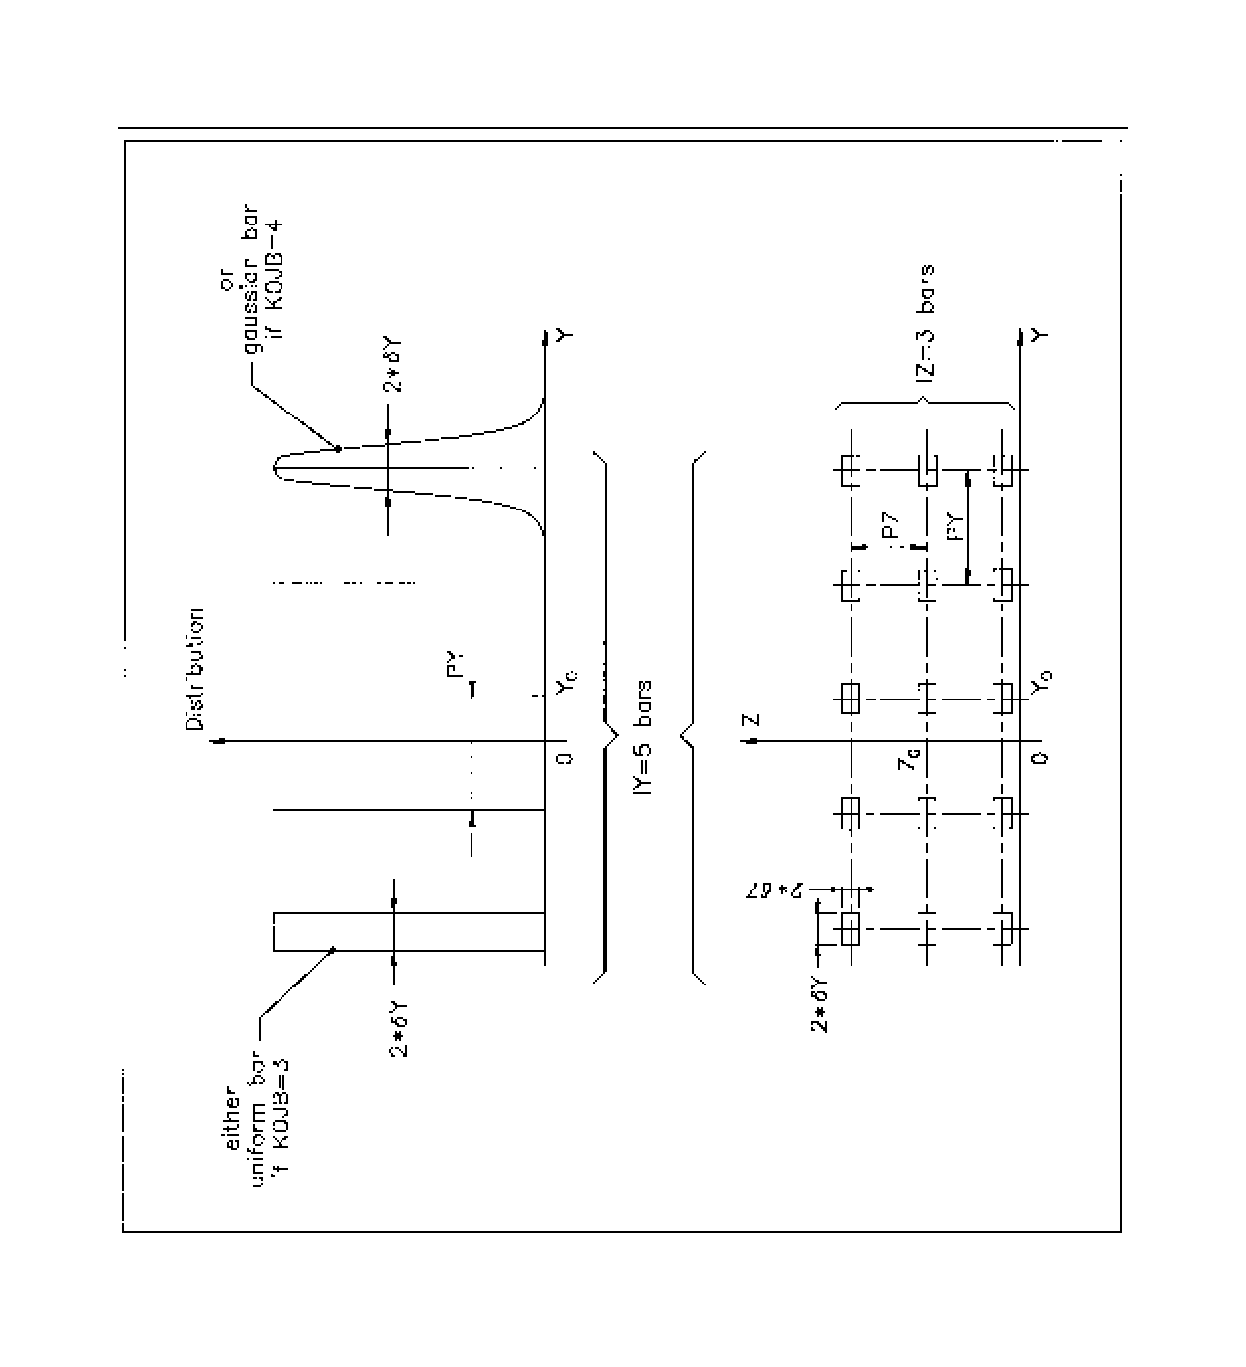
\includegraphics[width=15cm,angle=-90]{Fig5.ps}}  %% now 6
	\hangcaption[Fig5]{\label{fig5}Scheme of the input parameters to \textsl{MCOBJET} 
	when \KOBJ = 3, 4\\
   A~: A distribution of the $ Y $ coordinate\\ 
B~: A 2-D grid in ($ Y, Z $) space.} 
 \end{figure}
 \vfill 

\newpage

 
\subsubsection*{OBJET~:   \OBJETTitl} \label{OBJET} \index{OBJET}
\index{negative charge}\index{negative momentum}

\textsl{OBJET} is dedicated to the determination of the initial
coordinates, in several ways.  
\medskip

\noindent The first datum is the reference rigidity (a negative value is 
allowed)
 
$$ \BORO = \dfrac{p_0 }{ q}  $$\index{BORO@{\BORO}}

\noindent At the object, the beam is defined by a set of particles (maximum~\imax) with 
the initial conditions ($ Y$, $T$, $Z$, $P$, $X$, $D$)  where $ D $ 
is the relative momentum. 

\noindent Depending on the value of the next datum \textsl{KOBJ}, these initial
conditions may be generated   in six different ways~:   
\bigskip

\noindent\textbf{KOBJ  =  1}~:  Defines a grid in the $ Y$, $T$, $Z$, $P$, $X$, $D$
 space. One gives the number of points desired,
 
 \begin{gather*}
	 IY,\quad IT,\quad IZ,\quad IP, \quad IX, \quad ID\\
\intertext{(maximum \ntm\ in each coordinate~: $ IY\leq \ntm\ \ldots ID\leq \ntm$ and 
such that $ IY * IT * ... * ID\leq \imax$) and the
		sampling size} 
	 PY,\quad PT,\quad PZ,\quad PP,\quad PX, \quad PD  
 \end{gather*}


\noindent\zgou\  then generates 
$ IY  \ast  IT  \ast  IZ \ast   IP \ast IX \ast  ID $ ($\leq  \imax$) initial conditions with the 
following coordinates

$$
  \begin{array}{*{5}{r<{,}}}
	  0  &  \pm PY &   \pm 2  \ast   PY & \ldots & \pm IY/2  \ast   PY \\
	  0  &  \pm PT &   \pm 2 \ast   PT  & \ldots &  \pm IT/2  \ast   PT \\
	  0  &  \pm PZ &   \pm 2 \ast  PZ   & \ldots &  \pm IZ/2 \ast PZ \\
	  0  &  \pm PP &   \pm 2  \ast PP  & \ldots  &  \pm IP/2  \ast  PP \\
	  0  &  \pm PX &   \pm 2  \ast  PX & \ldots  &  \pm IX/2 \ast   PX \\
 	  0  &  \pm PD &   \pm 2  \ast  PD & \ldots  &  \pm ID/2 \ast   PD 
 \end{array}
 $$

\noindent In this option relative momenta will be classified automatically for
the purpose of the use of \IMAGES\index{IMAGES} for momentum analysis.


\noindent The particles are tagged with an index \textsl{IREP} possibly
indicating a symmetry with respect to the ($ X$,$Y$) plane, as explained in option 
\mbox{\KOBJ= 3}. If two trajectories have mid-plane symmetry, only one  will be 
ray-traced, while the other will be deduced using the mid-plane 
symmetries. This is done for the purpose of saving computing time. It may 
be incompatible with the use of some procedures (e.g.~\textsl{MCDESINT\index{MCDESINT}}, which 
involves random processes). 

\noindent The last datum is the reference of the problem ($YR,TR,ZR,PR,XR,DR$). 
For instance the reference rigidity is $ DR \ast$ \BORO, resulting 
 in the rigidity of a particle of initial condition $ I\ast PD $ to be 
$ (DR+I\ast PD)\ast \BORO$. 

\bigskip

\noindent\textbf{KOBJ = 1.01}: Same as \KOBJ = 1    except for the $ Z $
symmetry.  The initial 
$ Z $ and $ P $ conditions are the following 

$$
  \begin{array}{*{5}{r<{,}}}
	  0  &  \pm PZ &   \pm 2  \ast   PZ & \ldots & \pm (IZ-1)   \ast   PZ \\
	  0  &  \pm PP &   \pm 2 \ast   PP  & \ldots &  \pm (IP-1)  \ast   PP 
  \end{array}
 $$


\noindent This object results in shorter outputs/CPU-time when studying problems with $Z $ symmetry.  

\bigskip

\noindent\textbf{KOBJ = 2~:}  Next data~: \IMAX\index{IMAX@{\IMAX}|textbf},  
\IDMAX\index{IDMAX@{\IDMAX}|textbf}. Initial coordinates
are entered explicitly for each 
trajectory.  \IMAX\  is the total number of particles (\IMAX$\leq \imax$).  
These may be classified in groups of equal number for each value of momentum, in order to 
fulfill the requirements of image calculations by \textsl{IMAGES\index{IMAGES}}. 
 \IDMAX\index{IDMAX@{\IDMAX}} is the 
number of groups of momenta.  The  following initial 
conditions defining a particle are specified for each one of the \IMAX\  
 particles
 $$ Y,\quad T,\quad Z,\quad P, \quad X, \quad D,\quad ^\prime A^\prime $$
%
 where $ D\ast \BORO$ is the rigidity (negative value   
 allowed) and $ ^\prime A^\prime $ is a
(arbitrary) tagging character.  


\noindent The last record \IEX\index{IEX@{\IEX}|textbf} (I=1, \IMAX)  contains 
\IMAX\  times either the string ``1'' (which indicates that the particle will be
tracked) or the string ``\mbox{-9}''  (indicates that the particle should not be tracked).  

\noindent This option \mbox{\KOBJ= 2}   may be be useful for the
definition of objects including kinematic  effects.  
\bigskip


\newpage 


\noindent\textbf{KOBJ $= 3$~:} This option allows the reading of initial conditions from an
external input file \textsl{FNAME}.  

\noindent The next three data lines are~: 

\smallskip 

IT1, IT2, ITStep

IP1, IP2, IPStep

YF,TF,ZF,PF,SF,DPF,TiF,TAG

YR,TR,ZR,PR,SR,DPR,TiR

InitC

\smallskip 

\noindent followed by the storage file name \textsl{FNAME}. 

\smallskip 

\noindent IT1, IT2, ITStep tell the code to read coordinates of particles number IT1 through  IT2 by step ITStep. 

\smallskip 

\noindent IP1, IP2, IPStep  tell the code to read coordinates belonging in the sole pass   IP1 through  IP2 by step IPStep. 
Indeed, IP2 $>$ IP1 assumes prior filling of \textsl{FNAME} in the course of a run (e.g., multiturn tracking) 
involving  the keyword \textsl{REBELOTE}. 

\smallskip 

\noindent YF, TF, ZF, PF, SF, DPF, TiF are references added to the  values of respectively Y, T, Z, P, S, DP as read 
from \textsl{FNAME}, whereas 
 YR, TR, ZR, PR, SR, DPR, TiR are scaling factors, so that any coordinate $C=Y,T,Z...$ is chenged into CF*C + CR. 
In addition a flag character TAG allows retaining only particles with identical tagging letter LET, unless 
TAG='*' in which case it has no selection effect - for instance TAG='S' can be used to retain only secondary 
particles following in-flight decay simulations. 

\smallskip 

\noindent 
If \mbox{InitC$=1$} ray-tracing starts from the current coordinates$ F(J,I)$, \\
if \mbox{InitC$=0$}  ray-tracing starts from the initial coordinates $ FO(J,I)$ as read from \textsl{FNAME}. 

\smallskip 


The  file \textsl{FNAME} must be formatted so as to fit the following \FORTRAN sequence 
\begin{alltt}
\footnotesize
         OPEN (UNIT = NL, FILE = FNAME, STATUS = `OLD')
	 DO 1 I = 1, IMAX
	    READ (NL,100) LET (I), IEX(I), (FO(J,I),J=1,6), (F(J,I),J=1,6), I, IREP(I),
     >      LET(I),IEX(I),-1.D0+FO(1,I),(FO(J,I),J=2,MXJ),
     >      -1.D0+F(1,I),F(2,I),F(3,I),
     >      (F(J,I),J=4,MXJ),ENEKI,
     >      ID,I,IREP(I), SORT(I),D,D,D,D,RET(I),DPR(I),
     >      D, D, D, BORO, IPASS, KLEY,LBL1,LBL2,NOEL
 100        FORMAT(1X,
C1   LET(IT),KEX,   1.D0-FO(1,IT),(FO(J,IT),J=2,MXJ),
     1           A1,1X,I2,1P,7E16.8,
C2   1.D0-F(1,IT),(FO(J,IT),J=2,MXJ),
     2         /,3E24.16,
C3   Z,P*1.D3,SAR,     TAR,     DS,
     3         /,4E24.16,E16.8,
C4   KART,  IT,IREP(IT),SORT(IT),X, BX,BY,BZ, RET(IT), DPR(IT),
     4         /,I1,2I6,7E16.8,
C5        EX,EY,EZ, BORO,  IPASS,  KLEY,  (LABEL(NOEL,I),I=1,2),NOEL
     5  /,4E16.8,          I6,1X,  A8,1X,  2A10,                I5)
    1    CONTINUE
\end{alltt} 

\noindent where the meaning of the parameters (apart from D=dummy real, ID=dummy integer) is the following   
\medskip
 
\begin{tabular}{>{\sl}l!{:}p{10cm}}
LET(I) & one-character string (for tagging)  \\
 IEX(I)\index{IEX@{\IEX}} &  flag, see \KOBJ = 2  \\
 FO(1-6,I) &  coordinates $ D$, $Y$, $T$, $Z$, $P $ and path length of the 
particle number $I$,  at the origin. $ D\ast \BORO $ = rigidity \\
F(1-6,I) & idem, at the current position.
\end{tabular}
\medskip

\noindent\textsl{IREP}   is an index which indicates a symmetry with
respect to median plane.  For instance, if $ Z(I+1)=-Z(I), $ then normally 
\textsl{IREP}$(I+1)=$ \textsl{IREP}$(I)$.
Consequently the coordinates of particle $ I+1 $ will not be obtained from 
ray-tracing but instead deduced without ray-tracing  from those of 
particle $ I $ by simple symmetry.  This results in gain of computing time.

\bigskip

\noindent\KOBJ $= 3 $    can be used directly for reading files filled by \textsl{FAISCNL}, \textsl{FAISTORE}.\\
If more than \imax\ particles are to be read from a file, use 
\IMAX\index{IMAX@{\IMAX}}$\leq \imax$  in conjunction with \textsl{REBELOTE\index{REBELOTE}}.   

\bigskip\noindent
In this case (but not \textbf{KOBJ = 3.01} or \textbf{KOBJ = 3.02}),
particles will not have the reference
charge and PARTICUL will not assign a mass or charge.

\bigskip

\noindent\textbf{KOBJ = 3.01:} Same as \textbf{KOBJ = 3}, except for the formatting of trajectory coordinate 
data in  \textsl{FNAME} which is much simpler, namely, according to the following \FORTRAN sequence 
\begin{alltt}
\footnotesize
         OPEN (UNIT = NL, FILE = FNAME, STATUS = `OLD')
    1    CONTINUE
         READ (NL,*,END=10,ERR=99) Y, T, Z, P, S, D
         GOTO 1
   10    CALL ENDFIL
   99    CALL ERREAD
\end{alltt} 

\bigskip

\noindent\textbf{KOBJ = 3.02:} As for \textbf{KOBJ=3.01}, except the format
is 
\begin{alltt}
         READ(NL,*) X,Y,Z,PX,PY,PZ
\end{alltt}
where \texttt{PX}, \texttt{PY}, and \texttt{PZ}, are the momenta in
MeV/$c$.  Note that DPR will be ignored in this case.
\bigskip

\noindent\textbf{KOBJ = 3.03:} As for \textbf{KOBJ=3.01}, except the format
is 
\begin{alltt}
         READ(NL,*) DP,Y,T,Z,P,S,TIME,MASS,CHARGE
\end{alltt}
where \texttt{MASS} is the mass in MeV/$c$ and \texttt{CHARGE} is the
charge divided by $e$.  In this case, particles will not have the reference
charge and \textsl{PARTICUL} will not assign a mass or charge.
\bigskip


\noindent\textbf{KOBJ = 5~:} Mostly dedicated to the calculation of first order
transfer matrix and various other  optical parameters 
 in conjunction with \textsl{MATRIX\index{MATRIX}} or with \textsl{TWISS\index{TWISS}}.  
The input data are the stepsizes 
\smallskip
$$ PY,\quad PT,\quad PZ,\quad PP, \quad PX, \quad PD $$

\noindent The code generates  11 particles 
$$ 0,\quad \pm PY,\quad \pm PT,\quad \pm PZ,\quad \pm PP, \quad \pm PX, \quad \pm PD $$

\noindent These values should be small enough, so that the paraxial ray
approximation be valid. 

\noindent The last data are the initial coordinates of the reference 
trajectory [normally $(YR, TR, ZR, PR, XR, DR) = (0, 0, 0, 0, 0, 1)$]. 
The reference rigidity  is $ DR\ast \BORO$ 
(negative value allowed).  

\bigskip

\noindent\textbf{KOBJ = 5.01:} Same as \textbf{KOBJ = 5}, except for an additional data line giving 
initial beam ellipse parameters $\alpha_Y, \beta_Y$, $\alpha_Z, \beta_Z$, $\alpha_X, \beta_X$,  
 for further transport of these using \textsl{MATRIX}, or for  possible use by the \textsl{FIT}\index{FIT} procedure. 

\bigskip

\noindent\textbf{KOBJ = 5.NN:} Like \textbf{KOBJ = 5}, except that instead of
just one set of initial coordinates, the input file contains \textbf{NN} sets
of initial coordinates.  For example, to have 6 sets of initial coordinates,
\textbf{KOBJ} should be \textbf{5.06}.

\bigskip

\noindent\textbf{KOBJ = 6:}  Mostly dedicated to the calculation of first, second
and other higher order transfer coefficients and various other  optical parameters, 
in conjunction with \textsl{MATRIX\index{MATRIX}} or with \textsl{TWISS\index{TWISS}}. 
The input data are the step sizes 

$$ PY,\quad PT,\quad PZ,\quad PP, \quad PX, \quad PD $$
 
 \noindent to allow the building up of an object containing 61 particles.  The
last data are the initial coordinates of the reference 
trajectory [normally $(YR, TR, ZR, PR, XR, DR) = (0, 0, 0, 0, 0, 1)$]. 
The reference rigidity of the beam  is $ DR\ast \BORO$.  

\bigskip


\noindent\textbf{KOBJ = 7~:} Object with kinematics 

\noindent The data and functioning are the same as for \mbox{\KOBJ= 1}, except for the 
following  
\begin{itemize}
\item[$\bullet$]  $ ID $ is not used,  
\item[$\bullet$]  $ PD $ is the kinematic coefficient, such that for particle
number $ I$,  the initial relative momentum $ D_I $ is calculated from the initial angle 
$T_I $ following
$$ D_I = DR+ PD \ast  T_I $$
 while $ T_I $ is in the range
$$ 0,\quad \pm PT,\quad \pm 2\ast PT,\quad \ldots,\quad \pm IT/2\ast PT $$
 as stated under \KOBJ = 1
\end{itemize}


\noindent\textbf{KOBJ = 8~:} Generation of phase-space coordinates on ellipses. 

\noindent The ellipses are defined by  the three sets of data (one set per 
  ellipse) 

$$
\begin{array}{*{2}{r<{,}}r}
 \alpha_ Y  &   \beta_ Y  
            &  \varepsilon_Y / \pi \\
\alpha_ Z   &  \beta_ Z  
            &  \varepsilon_Z / \pi \\
\alpha_ X   & \beta_ X 
            &  \varepsilon_X / \pi 
\end{array}           
$$            
%
where $\alpha$, $\beta$ are the ellipse parameters and $\varepsilon/ 
\pi$ is the emittance encompassed, corresponding to an ellipse with equation 
$\dfrac{1 + \alpha^2_Y}{\beta_Y} Y^2 + 2 \alpha_Y YT + \beta_Y T^2 = 
\varepsilon_Y / \pi$ (idem for the ($Z, P$) or ($X, D$) planes). 

\noindent The ellipses are centered respectively on $(Y_0, T_0)$, $(Z_0, P_0)$, $(X_0, D_0)$.  

\noindent The number of samples per plane is respectively $IX, IY, IZ$.  If that value is zero, 
the central value above is assigned. 
 

\newpage


\subsubsection*{OBJETA~:   \OBJETATitl\ \protect\cite{Biblio9}}  %%% [9]
 \label{OBJETA} \index{OBJETA}\index{Monte Carlo}
 
This generator simulates the reactions 

\begin{gather*}
     M_1+M_2 \longrightarrow  M_3+M_4  \\
\intertext{and then} 
     M_4 \longrightarrow  M_5 + M_6 
\end{gather*}
%
where  $ M_1 $ is the mass of the incoming body~; $ M_2 $ is the mass
of the target~;  $ M_3 $ is an outgoing body~;  $ M_4 $ is the rest mass of the
decaying body~; $ M_5 $ and $ M_6 $ are decay products. Example~: 

  \begin{gather*}
	  p+d \longrightarrow^3 \text{He}  + \eta  \\
	 \eta  \longrightarrow  \mu^ ++ \mu^-
  \end{gather*}
   
\noindent The first input data are the reference rigidity 

$$ \BORO = \dfrac{p_0 }{ q} $$\index{BORO@{\BORO}}

\noindent an index \textsl{IBODY} which specifies the particle to be ray-traced, namely
M3 (\textsl{IBODY} = 1),  M5 (\textsl{IBODY} = 2) or M6 (\textsl{IBODY} = 3).  In this last case, 
initial conditions for M6 must be generated by a first run of \textsl{OBJETA\index{OBJETA}} with 
\mbox{\textsl{IBODY} = 2}~;  they are then stored in a buffer array, and restored as initial conditions
at the next occurrence of \textsl{OBJETA\index{OBJETA}} with \mbox{\textsl{IBODY} = 3}. Note that
\zgou\ by default assumes positively charged particles.  
\bigskip

\noindent Another index, \KOBJ specifies the type of
distribution for the initial transverse coordinates $ Y$, $Z $~;   
namely either uniform (\KOBJ = 1) or Gaussian 
(\KOBJ = 2).  The other three coordinates $ T$, $P$ and $ D $ are 
deduced from the kinematic of the reactions.   
\bigskip

\noindent The next data are the number of particles to be generated, 
\IMAX\index{IMAX@{\IMAX}}, and the masses involved  in the two previous
reactions. 
 
 $$ M_1,\quad M_2,\quad M_3,\quad M_4,\quad M_5,\quad M_6 $$
%
 and the kinetic energy $ T_1 $ of the incoming body ($M_1$). 
 
\noindent Then one gives the central value of the distribution for each
coordinate 

\begin{gather*}
	Y_0,\quad T_0,\quad Z_0,\quad P_0,\quad D_0    \\
\intertext{and the width of the distribution around the central value }
	 \delta Y,\quad \delta T,\quad \delta Z,\quad \delta P,\quad \delta D \\
\intertext{so that only those particles in the range }
	Y_0-\delta Y\leq Y\leq Y_0+\delta Y\qquad \ldots \qquad D_0-\delta
	D\leq D\leq D_0+\delta D  \\
\intertext{will be retained.  The longitudinal initial coordinate is uniformly
	sorted in the range }
	 -\XL \leq  X_0 \leq  \XL 
\end{gather*}
 
\noindent The random sequences involved may be initialized with different
values of the 
two integer seeds $ IR_1 $ and $ IR_2 $ ($\simeq 10^6 $). 

\bigskip\noindent \textsl{PARTICUL\index{PARTICUL}} will not change the masses
that are assigned by \textsl{OBJETA}.

\newpage

\subsection{Declaration of options} \label{sec4.3}

These options allow the control of procedures that affect certain 
functions of the code. Some options are normally declared right after 
the object definition (e.g.~\textsl{SPNTRK\index{SPNTRK}} - spin tracking, 
\textsl{MCDESINT\index{MCDESINT}} -
in-flight decay),  others are normally declared at the end of the data pile (e.g. 
\textsl{END\index{END}} -- end of a problem, 
\REBELOTE\index{REBELOTE} -- for tracking more than \imax\~particles  or for 
multi-turn tracking, 
\textsl{FIT\index{FIT}} -- fitting procedure). 

\newpage

\subsubsection*{BINARY~: \BINARYTitl}  \label{BINARY} \index{BINARY|textbf}
\medskip

This procedure translates field map data files from ``BINARY'' to 
``FORMATTED'' -- in the \FORTRAN sense, or the other way.
\bigskip

\noindent The keyword is followed, next line, by NF.NCOL ($NF\leq9$, $NCOL\leq9$), the number of files to be translated and 
of data columns in the file.  NCOL should be consistant with the following FORTRAN READ statement~: 

       {\tt     READ (unit=ln,*) (X7(I),I=1,NCOL)}

\noindent The first data line in a field map file is a header, 
and contains $NCOL$ reals as reference X coordinate, mesh step $\delta X$, 
reference Y coordinate, mesh step $\delta Y$, and three others (see the FMAPW FORTRAN procedure for 
more datails).
 
\noindent Then follow, line per line, the NF names of the files to be translated.
\medskip

\noindent Iff a file name begins with the prefix ``B\_'' or ``b\_'', it is 
presumed ``binary'', and hence converted to ``formatted'', and given 
the same name after suppression of the prefix ``B\_'' or ``b\_''. Conversely, 
{\it iff} the file name does not begin with ``B\_'' or ``b\_'', the file is 
presumed ``formatted'' and hence translated to ``binary'', and is 
given the same name after addition of the prefix ``B\_''.
\medskip

\noindent In its present state, the procedure \textsl{BINARY} 
only supports a limited number of output formatting, e.g. from  \textsl{TOSCA}\index{TOSCA} magnet code 
 (see keyword \textsl{TOSCA}\index{TOSCA}). 


\newpage

\subsubsection*{END or FIN~: \ENDTitl}  \label{FIN} \index{FIN|textbf} \label{END} \index{END|textbf}
\medskip

The end of a problem, or of a set of several problems stacked in 
the data file, should be stated by means of the keywords \textsl{FIN} or
\textsl{END}.  
\bigskip

\noindent Any information following these keywords will be ignored. 

\newpage

\subsubsection*{FIT, FIT2~:  \FITTitl}  \label{FIT}  \label{FIT2} \index{FIT|textbf} \index{FIT2|textbf}
\medskip

 The keywords \textsl{FIT, FIT2} allow the automatic adjustment of up to 20 
variables\index{variable (FIT)}, for fitting up to 20 constraints\index{constraint (FIT)}. 

\noindent \textsl{FIT} has been implemented  recently~\cite{NedlerMead} and has various advantages over the original method, 
as converging speed. The  older \textsl{FIT2} 
was drawn from  the matrix transport code BETA~\cite{Biblio10}. 

\noindent Any physical parameter of any element (\emph{i.e.}~keyword) may 
be varied. Available constraints  are, amongst others~:  any of the $6 \times 6$
coefficients of the first order transfer matrix $ \lbrack R_{ij}\rbrack $ as defined in the
keyword \textsl{MATRIX\index{MATRIX}}, and its horizontal $ (R_{11 }R_{22} -R_{12} R_{21}) $ and
vertical $ (R_{33} R_{44}- R_{34} R_{43}) $ determinants~; horizontal and vertical tunes (if 
periodical structure)~;  any of the
$6\times 6 \times6 $ coefficients of the second order array $ \lbrack T_{ijk}\rbrack $ 
as defined in \textsl{MATRIX\index{MATRIX}}~; any of the $ 2 \times 4 $ coefficients of the 
\mbox{$\sigma$-matrix} as defined by
%
$$ \lbrack \sigma_{ ij}\rbrack  = 
\begin{pmatrix}
	\sigma_{11} &  \sigma_{12} &   &  \\
	 \sigma_{21} &  \sigma_{22} &  & \\
	             &               &  \sigma_{33} & \sigma_{34} \\
	             &               & \sigma_{43} & \sigma_{44} 
\end{pmatrix}
$$
%
 and any trajectory coordinates $ F(J,I) $ as defined in \textsl{OBJET} 
($ I $  =  particle number, $ J $  = coordinate number = 1 to 6 for 
respectively $ D$, $Y$, $T$, $Z$,$ P $ or $ S= $path length). 

\noindent Tunes $\nu_{Y,Z}$ and Twiss\index{TWISS} periodic functions $\beta_{Y,Z}, \alpha_{Y,Z}, \gamma_{Y,Z}$ are adjustable 
as well~; they are defined by identification of the full optical structure transfer matrix  
$  \lbrack R_{ij}\rbrack $  with the Twiss matrix, following 
  $\lbrack R_{ij}\rbrack = I cos(2 \pi \nu_{Y,Z}) + J sin (2 \pi \nu_{Y,Z}) $ wherein 
$J=\left( \begin{array}{cc} \alpha & \beta \\ -\gamma& -\alpha \end{array} \right) $.  

\paragraph{\textit{VARIABLES}}\index{variable (FIT)|textbf}

\noindent The first input data in \textsl{FIT\index{FIT}} are the number of variables
\textsl{\NV}, and for each one of them, the following parameters  

\begin{tabular}{ll}
$ IR = $ &number of the varied element in the structure \\
$ IP =  $ &number of the physical parameter to be varied in this element \\
$ XC =  $ &coupling parameter. Normally $ XC=0$.  If $ XC\not= 0$, coupling will occur (see below).\\
$ DV = $ &allowed relative range of variation of the physical parameter $ IP $.
\end{tabular}

\paragraph{Numbering of the elements (\textsl{IR})~: } 

\noindent The elements (\textsl{DIPOLE\index{DIPOLE}, QUADRUPO\index{QUADRUPO},} etc.) are numbered
following their sequence in the \zgou\ input data file, for the purpose of 
the \textsl{FIT\index{FIT}} procedure. The number of any element just identifies with 
its position in the data sequence. However, a simple way to get $ IR $ is to make a preliminary run~: \zgou\ will then
print the whole structure into the file  zgoubi.res with all elements numbered.  
%\bigskip

\paragraph{Numbering of the physical parameters (\textsl{IP})~: }

\noindent In the elements  \textsl{DIPOLE\index{DIPOLE}}, \textsl{AIMANT\index{AIMANT}} 
and \textsl{EBMULT\index{EBMULT}}, \textsl{ELMULT\index{ELMULT}}, \textsl{MULTIPOL\index{MULTIPOL}}, the
numbering of the physical parameters just follows their sequence, as it is shown here after 
for \textsl{DIPOLE-M}~: the left column below represents the input data, the 
right one the corresponding numbering to be used for the \textsl{FIT\index{FIT}} procedure. 
\begin{center}
{\renewcommand{\arraystretch}{1}
	\begin{tabular}{lcl}
	\textbf{Input  data}  &~~~~~~~~&  \textbf{Numbering  for  FIT}\\
      \textsl{DIPOLE-M}                      \\
	\textsl{NFACE,  \IC,  \IL}     &  &  1, 2, 3 \\
	\textsl{IAMAX,  IRMAX}         &&  4, 5    \\
	$B_0$, $N$, $B$, $G$  &&  6, 7, 8, 9\\
	\textsl{AT, ACENT, RM, RMIN, RMAX} &&  10, 11, 12, 13, 14 \\
	$\lambda$ , $\xi$     &&  15,16    \\
	$\NC$, $C_0$, $C_1$, $C_2$, $C_3$, $C_4$, $C_5$ shift
	                      &&  17, 18, 19, 20, 21, 22, 23, 24\\
	$\omega$, $\theta$, $R_1$, $U_1$, $U_2$, $R_2$ 
	                      && 25, 26, 27, 28, 29, 30 \\
	etc.                 && etc.
	\end{tabular}   }
\end{center}

\newpage %%%

\noindent Parameters in \textsl{SCALING\index{SCALING}} also have a specific numbering, as follows. 
\begin{center}
{\renewcommand{\arraystretch}{1}
	\begin{tabular}{lcl}
	\textbf{Input  data}  &~~~~~~~~&  \textbf{Numbering  for  FIT}\\
      \textsl{SCALING}                      \\
	\textsl{IOPT, NFAM }      & &  \\
	\textsl{NAMEF}         &&    \\
	$NT_1$    &      &            \\
	$SCL(I)$, $I=1$, $NT_1$ &&  10 $[,...,~10+NT_1]$ \\
	$TIM(I)$, $I=1$, $NT_1$ &&  10 $[,...,~10+2*NT_1]$ \\
	\textsl{NAMEF}        & &    \\
	$NT_2$    &               &   \\
	$SCL(I)$, $I=1$, $NT_2$ &&  20 $[,...,~20+NT_2]$ \\
	$TIM(I)$, $I=1$, $NT_2$ &&  20 $[,...,~20+2*NT_2]$ \\
          {\Large...}   \\
	etc.  up to \textsl{NFAM}       &        & etc.
	\end{tabular}   }
\end{center}

\noindent For all other keywords, the parameters are numbered in the 
following way 
\begin{center}
{\renewcommand{\arraystretch}{1}
	\begin{tabular}{lcl}
	\textbf{Input  data}  &~~~~~~~~&  \textbf{Numbering  for  FIT}\\
	KEYWORD      &&  \\
	first line   && 1, 2, 3,...\\
	second  line &&  10, 11, 12, 13,...\\
	this  is  a  comment &&  a line of comments is skipped\\
	next line    && 20, 21, 22,...  \\
	and  so  on... && 30, 31, 32, 33,... 
	\end{tabular}    }
\end{center}


\noindent The examples of \textsl{QUADRUPO\index{QUADRUPO}} (quadrupole) and 
\textsl{TOSCA\index{TOSCA}} (Cartesian or cylindrical mesh field map) are given below.

\begin{center}
{\renewcommand{\arraystretch}{1}
	\begin{tabular}{lcl}
	\textbf{Input  data}  &~~~~~~~~&  \textbf{Numbering  for  FIT}\\
	\textsl{QUADRUPO}\index{QUADRUPO}        \\
    $\IL$                                                   & &     1\\
    $\XL$, $R_0$, $B$                                       && 10, 11, 12 \\
    $X_E$, $\lambda_E$                                      && 20, 21 \\
    \textsl{\NCE}, $C_0$, $C_1$, $C_2$, $C_3$, $C_4$, $C_5$  && 30, 31, 32, 33, 34, 35, 36 \\
    $X_S$, $\lambda_S$                                      && 40, 41 \\
    \textsl{\NCS}, $C_0$, $C_1$, $C_2$, $C_3$, $C_4$, $C_5$  &&  50, 51, 52, 53, 54, 55, 56 \\
   \textsl{XPAS}                                            &&  60\\
   \textsl{KPOS, XCE, YCE, ALE }                            && 70, 71, 72, 73 \\
   \\
   \textsl{TOSCA}  \\
   \textsl{\IC, \IL}  &  &  1, 2\\
   \textsl{BNORM, X- [, Y-, Z-]NORM}     &&  10, 11 [, 12, 13] \\
   \textsl{TIT}       &&  This is  text \\
   $IX$,  $IY$, $IZ$, \textsl{MOD} &&  20, 21, 22, 23  \\
   \textsl{FNAME}     && This is  text \\
   $ID$, $A$, $B$, $C$  [$A^\prime$, $B^\prime$, $C^\prime$, etc. if $ID \geq  2$]
             &&  30, 31, 32, 33 [34, 35, 36 [, 37, 38, 39] if $ID \geq  2$]  \\
   \textsl{IORDRE}    &&  40   \\
   \textsl{XPAS}      && 50    \\
   \textsl{KPOS, XCE, YCE, ALE } 
             && 60,61,62,63
\end{tabular}  }
\end{center}             
             
\newpage

\paragraph{Coupled variables  ($XC$)} 

\noindent  Coupling a variable parameter to any other parameter in the
structure is possible. This is done by giving $XC$ a value of the form $ r \cdot ppp $ where
the integer part $ r $ is the number of the coupled element in the structure 
(equivalent to $ IR$, see above), and the decimal part $ ppp $ is the number of its 
parameter of concern (equivalent to $ IP$,  see above) (if the parameter
number is in the range 1, 2, ... ,9 (resp. 10, 11, ... 19 or 100, ...), then $ ppp $ 
must take the form $ 00p$ (resp. $0pp$, $ppp$)). For example, $ XC=20 \cdot 010 $ is a request for coupling with the
parameter number~10 of element number~20 of the structure, while $ XC=20 \cdot 100 $
is a request for coupling with the parameter number~100 of element~20.  

\bigskip

\noindent An element of the structure which is coupled (by means of $ XC\not= 0) $ to a 
variable declared in the data list of the \textsl{FIT\index{FIT}} keyword, needs not appear 
as one of the $ \NV $ variables in that data list (this would be redundant information).  

\smallskip

\noindent$ XC $ can be either positive or negative. If $ XC>0$,  then the
coupled parameter will be given the same value as the variable parameter  
(for example, symmetric 
quadrupoles in a lens triplet will be given the same field). If $ XC<0$, 
then the coupled parameter will be given a variation opposite to that of the
variable, so that the sum of the two parameters stays constant (for example, an optical 
element can be shifted while preserving the length of the structure, by coupling 
together its upstream and downstream drift spaces).  


\smallskip
 
\paragraph{Variation range  ($DV$)} 

\noindent For a parameter $ IP $ of initial value $ p $, the \textsl{FIT}\index{FIT} procedure is
allowed to explore the range $ p(1\pm DV)$.   

\smallskip

\begin{center}
	\begin{tabular}{lcp{10cm}}
	$\IC$        &  = &  type of  constraint (see table below).\\
	$I$, $J$    & =  &  constraint (\emph{i.e.}~$R_{ij}$, determinant, tune~; 
	                    $T_{ijk}$~; $\sigma_{ ij}$~; trajectory $\#I$ and coordinate $\#J$)\\
	$IR$       &  =  &  number of the element in the \zgou\ input data file, right after which 
	                    the constraint applies   \\
	$V$        &  =  &  desired value of the constraint\\
	$W$        &  =  &  weight of the constraint (smaller $W$ for higher weight)
	\end{tabular}
\end{center}



\smallskip

\paragraph{\textit{CONSTRAINTS}} \index{constraint (FIT)|textbf}

\noindent The next input data in \textsl{FIT\index{FIT}} are the number of constraints,
\textsl{\NC}, and for each one of them the following parameters.

\smallskip


\noindent {\it IC=0~: } The coefficients 
$ \sigma_{11}~(\sigma_{ 33}) = $ horizontal (vertical) beta values and 
$ \sigma_{ 22}~(\sigma_{ 44}) = $ horizontal (vertical) derivatives ($\alpha = -\beta'/2$) 
are obtained by transport of their initial values at line start as introduced using for instance  
\textsl{OBJET\index{OBJET}, KOBJ=5.1}.\\

\smallskip

\noindent  {\it IC=0.1~: } Twiss\index{TWISS} functions~: $\sigma_{11}=\beta_Y, \sigma_{12}=\sigma_{21}=-\alpha_Y, 
\sigma_{22}=\gamma_Y$, $\sigma_{33}=\beta_Z, \sigma_{34}=\sigma_{43}=-\alpha_Z, \sigma_{44}=\gamma_Z$~; periodic dispersion~: 
$\sigma_{16}=D_Y$, $\sigma_{26}=D'_Y$,  $\sigma_{36}=D_Z, \sigma_{46}=D'_Z$, all quantities derived by assuming 
 periodic structure and identifying the first order transfer matrix to its Twiss form. 



%  \newlength{\LL}
\settowidth{\LL}{\textbf{Beam matrix\ }}
\footnotesize
	\begin{center}
    {\renewcommand{\arraystretch}{1}
			\begin{tabular}{|>{\bfseries}p{\LL}|c|c|c|c|c|c|c|c|p{\LL}|}
			\hline
			\hline
			 \multirow{3}{\LL}{\textbf{Type of constraint}}
			    & \multicolumn{8}{c|}{\rule{0cm}{5mm} \textbf{Parameters defining the constraints}} 
                            &\multirow{3}{\LL}{\textbf{Object definition (recommended) }}  \\[-2mm]
			\cline{2-9}
			    & \rule{0cm}{5mm}$\mathbf{\IC}$ 
			    & $\mathbf{I}$ & $\mathbf{J}$ & \textbf{Constraint}  
                            &  \multicolumn{4}{c|}{\textbf{Parameter(s)}  } &   \\
         & & & & & \multicolumn{1}{c|}{\#} & \multicolumn{3}{c|}{  values} & \\
			\hline
                          & & & & & & & & &  \\
			   \multicolumn{1}{|c|}{\textbf{\mbox{$\sigma$-matrix} }} 
	 & 0& 1 - 6 & 1 - 6 & $\sigma_{IJ}$~~  ($\sigma_{11}=\beta_Y$, $\sigma_{12}=\sigma_{21}=\alpha_Y$, etc.) 
	 & & & & & \textsl{OBJET/KOBJ=5,6} \\
                          & & & & & & & & &  \\
			   \multicolumn{1}{|c|}{\textbf{Beam matrix }} 
	 & 0.N & 1 - 6 & 1 - 6 & $\sigma_{IJ}$~~  ($\sigma_{11}=\cos\mu_Y + \alpha_Y \sin\mu_Y$, etc.) 
	 & & & & & \textsl{OBJET/KOBJ=5,6} \\
			\multicolumn{1}{|c|}{\textbf{  }} & &  7 & any & Y-tune = $\mu_Y/2\pi$ & & & & & \\
			\multicolumn{1}{|c|}{ (N=1-9  for {\small \textsl{MATRIX}}} & & 8 & any & Z-tune = $\mu_Z/2\pi$ & & & & &  \\
			\multicolumn{1}{|c|}{  block 1-9))} & &  9 & any & $\cos(\mu_Y)$  & & & & &  \\
			\multicolumn{1}{|c|}{                       } & & 10 & any & $\cos(\mu_Z)$  & & & & &  \\
                           & & & & & & & & &  \\
			\multicolumn{1}{|c|}{\textbf{First order}}  
			    & 1  & $1 - 6$ & $1 - 6$ & Transport coeff. $R_{IJ} $  
	 & & & & & \textsl{OBJET/KOBJ=5} \\
			\multicolumn{1}{|c|}{\textbf{parameters}} &   & 7 & any & Y-determinant  & & & & &  \\
			\multicolumn{1}{|c|}{\textbf{ }}  &    & 8 & any  & Z-determinant  &  & & & & \\
                            & & & & & & & & &  \\
			\multicolumn{1}{|c|}{\textbf{Second order}}  
			    & 2  & $1 - 6$ & 1$1 - 6$6 & Transport coeff.  $T_{I,j,k} $  
	 & & & & & \textsl{OBJET/KOBJ=6} \\
			 \multicolumn{1}{|c|}{\textbf{parameters}} &  &  &  & $  (j= [J/10] ,k=J-10 [J/10] ) $  & & & & &  \\
			 \multicolumn{1}{|c|}{\textbf{ }}  &  &  &  &  &  & & & &  \\
                            & & & & & & & & &  \\
%
			\multicolumn{1}{|c|}{\textbf{Trajectory}}
			    & 3 & $1 - \IMAX$ & $1 - 7$  & $  F(J,I) $  
         & & & & & \textsl{[MC]OBJET}   \\
			 \multicolumn{1}{|c|}{\textbf{coordinates}}
			    &   &  $-1$      & $1 - 7$  &   $<F(J,i)>_{i=1,\IMAX}$ & & & & &   \\
			 \multicolumn{1}{|c|}{\textbf{ }}
			    &   &  $-2$      & $1 - 7$  &   $Sup(|F(J,i)|)_{i=1,\IMAX}$ &  & & & &   \\
			 \multicolumn{1}{|c|}{\textbf{ }}
			    &   &  $-3$      & $1 - 7$  &  $Dist|F(J,I)|_{i=I1,I2,dI}$ &  3 & I1 & I2 & dI &  \\
			\multicolumn{1}{|c|}{\textbf{  }}
			    & 3.1 & $1 - \IMAX$ & $1 - 7$  &$|F(J,I) - FO(J,I)|$  & & & & &   \\
			\multicolumn{1}{|c|}{\textbf{  }}
			    & 3.2 & $1 - \IMAX$ & $1 - 7$  &$|F(J,I) + FO(J,I)|$  & & & & &  \\
			\multicolumn{1}{|c|}{\textbf{  }}
			    & 3.3 & $1 - \IMAX$ & $1 - 7$  & min. (1) or max. (2) value of $F(J,I)$ & 1 & 1-2 & & &  \\
			\multicolumn{1}{|c|}{\textbf{  }}
			    & 3.4 & $1 - \IMAX$ & $1 - 7$  &$|F(J,I) - F(J,K)|$ ~ ($K=1 - \IMAX$) & 1 & K & & &  \\
                            & & & & & & & & &  \\
%
			\multicolumn{1}{|c|}{\textbf{Matched ellipse}} 
	 & 4 & $1 - 6$ & $1 - 6$ & $\sigma_{IJ}$~~  ($\sigma_{11}=\beta_Y$, $\sigma_{12}=\sigma_{21}=\alpha_Y$, etc.) 
	 & & & & & \textsl{OBJET/{\footnotesize KOBJ=8}~; }  \\
                          \multicolumn{1}{|c|}{\textbf{parameters}} & & & & 
         & & & & & \textsl{MCOBJET/{\footnotesize KOBJ=3}}  \\
                           & & & & & & & & &  \\
			\multicolumn{1}{|c|}{\textbf{Number of}} 
			    & 5 & $-1$ & any &  $N_{survived}/\IMAX$  
         & & & & & \textsl{OBJET} \\
			\multicolumn{1}{|c|}{\textbf{particles}} &  & $1 - 3$ & any 
                & $N_{in~\epsilon_{Y,Z,X}}/ N_{survived}$ 
         & 1 & $\epsilon/ \pi $& & & \textsl{MCOBJET}   \\
			    &  & $4 - 6$ & any 
                & $N_{in~best~\epsilon_{Y,Z,X,rms}}/ N_{survived}$ 
         & 1 & $\epsilon/ \pi $& & & \textsl{MCOBJET}   \\
                           & & & & & & & & &  \\
%
			\multicolumn{1}{|c|}{\textbf{Spin}}
			    & 10 & $1 - \IMAX$ & $1 - 4$  & $  S_{X,Y,Z}(I), ~ |\vec S(I)| $  
         & & & & & \textsl{[MC]OBJET}   \\
			\multicolumn{1}{|c|}{\textbf{  }}
			    & 10.1 & $1 -\IMAX$ & $1 -3$  &$|S_{X,Y,Z}(I) -SO_{X,Y,Z}(I)|$
         & & & & & \textsl{+SPNTRK}   \\
			\hline
			\hline
		\end{tabular}  }
	\end{center}
\normalsize


\smallskip


\noindent  {\it IC=1, 2~: }  The coefficients $ R_{ij} $ and $ T_{ijk} $ are calculated following
the procedures described in \textsl{MATRIX\index{MATRIX}}, option \mbox{\textsl{IFOC} = 0}. 
The fitting of the $ \lbrack R_{ij}\rbrack $ matrix coefficients or
determinants supposes the tracking of particles having initial coordinates 
sampled as described in \textsl{MATRIX\index{MATRIX}} (these particles are normally defined with 
\textsl{OBJET\index{OBJET}}, \mbox{\textsl{KOBJ} = 5 or 6}). The same is true for the $ T_{ijk} $
second order coefficients (Initial coordinates normally defined with \textsl{OBJET}, 
\mbox{\textsl{KOBJ} = 6}).  

\smallskip

\noindent  {\it IC=3~: } If $1<I<\IMAX$ then the value of coordinate type $J$ ($J=1,6$ for respectively 
 $D,~Y,~T,~Z,~P,~S$) of particle number $I$ ($1<I<\IMAX$) 
is constrained.  

Case $I=-1$~:  the constraint is the mean value of coordinate of type $J$. 

Case $I=-1$~:  the constraint is the max. value of coordinate of type $J$. 

Case $I=-1$~:  the constraint is the $J$-distance for two different particles. 

\smallskip

\noindent  {\it IC=3.1~: } Difference between final and initial $J$-coordinate of particle $I$ (convenient 
e.g. for closed orbit search). 

\smallskip


\noindent {\it IC=4~: } The coefficients 
$ \sigma_{11}~(\sigma_{ 33}) = $ horizontal (vertical) beta values and 
$ \sigma_{ 22}~(\sigma_{ 44}) = $ horizontal (vertical) derivatives ($\alpha = -\beta'/2$) 
are derived from an ellipse match of the current particle population (as generated for instance using 
\textsl{MCOBJET\index{MCOBJET}, KOBJ=3}).\\
%
The fitting of the $ \lbrack \sigma_{ij}\rbrack $ 
coefficients supposes the tracking of a relevant population of particles within an 
adequate emittance.  

\smallskip

\noindent  {\it IC=5~: } If $I=-1$ then  the constraint value is the ratio of particles still on the run. 
If $I\ge 1$ then the constraint value is the ratio of  particles encompassed within a given $I$-type 
($I=1-3$ for respectively $Y,~Z,~D$) phase-space surface. 

\smallskip

\noindent  {\it IC=10~: } If $1<I<\IMAX$ then the value of coordinate type $J$ ($J=1,3$ for respectively 
 $S_X, S_Y, S_Z$) of particle number $I$ ($1<I<\IMAX$) is constrained.  

\smallskip

\noindent  {\it IC=10.1~: } Difference between final and initial $J$-spin coordinate  of particle $I$ (convenient 
e.g. for closed orbit search). 





\paragraph{\textit{OBJECT DEFINITION}}


Depending on the type of constraint (see Table), constraint calculations are performed either from 
transport coefficient calculation and in such case need  \textsl{OBJET} with either \KOBJ~=~5  
or  \KOBJ~=~6, or from particle distributions and in this case need  object definition using for 
instance \textsl{OBJET} with \KOBJ~=~8,    \textsl{MCOBJET} with either \KOBJ~=~3. 

%\noindent Note that,  for constraint type $\IC = 3$, the object is normally defined 
%with keyword \textsl{OBJET}. If \KOBJ~$\not=~1$, any of the 1 to 
%\IMAX\ trajectories can be constrained. If \KOBJ = 2, only 
%the first seven trajectories can be constrained.


\smallskip

\paragraph{\textit{THE FITTING METHODS \protect\cite{NedlerMead,Biblio10}}}    %%%%[10]


\noindent The \textsl{FIT} procedure has been implemented  recently~\cite{NedlerMead} and 
has various advantages over the original method, as converging speed. 

\noindent The  older \textsl{FIT2} was drawn from  the matrix transport code BETA~\cite{Biblio10}. 
 The numerical procedure is a direct sequential minimization of the quadratic
sum of all errors (\emph{i.e.}, differences between desired and actual values of the $\NC$ 
constraints), each normalized by its specified weight $ W $ (the smaller $ W$,
the stronger the constraint). 

\noindent The step sizes for the variation of the physical parameters depend
on their initial  values, and cannot be accessed by the user. At each iteration, the 
optimum value of the step size, as well as the optimum direction of variation,
is determined for each one of the $\NV$ variables. Then follows an iterative
global variation of all $\NV$ variables, until the minimization fails which results in a
next iteration on the optimization of the step sizes. 

\newpage

\subsubsection*{GASCAT~: \GASCATTitl} \label{GASCAT}\index{GASCAT|textbf}
\medskip

Modification of particle momentum and velocity vector, performed at each integration step, 
under the effect of scattering by residual gas.

\bigskip

\noindent {\it To be documented}




\newpage

\subsubsection*{MCDESINT~: \MCDESINTTitl \protect\cite{Biblio11}}
              %%% [11]
\label{MCDESINT}\index{MCDESINT}\index{Monte Carlo}

 As soon as \textsl{MCDESINT}  appears in a structure
(normally, after \textsl{OBJET\index{OBJET}} or after \textsl{CIBLE\index{CIBLE}}),
 in-flight decay simulation starts. 
It must be preceded by \textsl{PARTICUL\index{PARTICUL}} for the definition of mass $ M_1 $ 
and \textsl{COM} 
lifetime $\tau_1$. 

\noindent The two-body decay simulated is 
 $$ 1 \longrightarrow  2+3 $$

\noindent The decay is isotropic in the center of mass. 
1~is the incoming particle, with mass $ M_1 $, momentum $ p_1=\gamma_1 M_1\beta_ 1c $ (relative 
momentum $ D_1= \dfrac{p_1 }{ q} \dfrac{1 }{\BORO} $ with \BORO   = reference
rigidity, see \textsl{OBJET\index{OBJET}}),  and position $ Y_1,Z_1 $ in the \zgou\ frame. 
2~and 3 are decay products with respective masses and momenta $ M_2, $ $ M_3 $ and 
$ p_2=\gamma_ 2M_2\beta_2c$,  $ p_3=\gamma_ 3M_3\beta_ 3c$.  

\noindent The decay length  $ s_1 $ of particle~1 is related to its center of 
mass lifetime $ \tau_ 1 $ by 
$$ s_1=c\tau_ 1 \sqrt{ \gamma^ 2_1 -1} $$

\noindent The path length $ s $ up to the decay point is then calculated from
a random number $ 0<R_1\leq 1 $ by using the exponential decay formula
$$ s = - s_1 \ell n R_1 $$

\noindent After decay, particle~2  will  be ray-traced with assumed positive
charge, while particle~3 is discarded.  Its scattering angles in the center of mass 
$ \theta^\ast $ and $\phi$ are generated from two other random numbers 
$R_2$ and $ R_3$. 
%$0<R_2\leq 1 $ and $ 0<R_3\leq 1 $ by
%
% \begin{alignat*}{2}
%	 \theta^ \ast 
%	       & =   2\pi (R_2 - 0.5) & \qquad & (-\pi   <\theta^\ast \leq \pi ) \\
%	\phi 
%	       & =   2\pi R_3         & \qquad &  (0<\phi \leq 2\pi ) 
% \end{alignat*}
%

$\phi$ is a relativistic invariant, and $\theta$ in the laboratory
frame (Fig.~\ref{fig6}) is given by    

$$ \tan \theta = \dfrac{1 }{ \gamma_1}\, 
    \dfrac{ \sin \theta^ \ast }{\dfrac{\beta_1 }{ \beta^ \ast_ 2}+ \cos \theta^\ast} 
    $$
%
  $ \beta^ \ast_ 2 $ and momentum $ p_2 $ are given by 

 \begin{align*}
	 \gamma^\ast_ 2 
	         & = \dfrac{M^2_1 + M^2_2 - M^2_3 }{ 2M_1M_2} \\
	\beta^\ast_ 2 
	         & =  \left( 1- \dfrac{1 }{ \gamma^ 2} \right)^{1/2} \\
	\gamma_2
	         & =   \gamma_1\gamma^ \ast_ 2 
	         	\left(1+\beta_1 \beta^\ast_ 2 \cos \theta^ \ast \right) \\
	p_2 
	         & = M_2 \sqrt{ \gamma^2_2 -1} 
 \end{align*}
 
\noindent Finally, $\theta$ and $\phi$ are transformed into the angles $ T_2 $
and $ P_2 $ in the \zgou\ frame, and the relative momentum takes the value 
$ D_2= \dfrac{p_2 }{ q} \dfrac{1}{\BORO} $ (where \BORO   
is the reference rigidity, see \textsl{OBJET\index{OBJET}}), while the starting position of 
$M_2 $ is $ Y_2=Y_1 $ and $ Z_2=Z_1 $.   
\bigskip

\noindent The decay simulation by \zgou\ obeys the following procedures.
In optical elements and field maps, after each integration step \textsl{XPAS}, the actual 
path length of the particle, $ F(6,I) $, is compared to its limit path length $ s$. 
 If $s $ is passed, then the particle is considered as having decayed at 
 $ F(6,I) - \dfrac{\text{\textsl{XPAS}} }{ 2} $, 
at a position obtained by a linear translation from the position at $ F(6,I)$.
[Presumably, the smaller \textsl{XPAS},  the smaller the error on position
and angles at the decay point].  
\bigskip
 %%%%%%%%%%%%%%figure%%%%%%%%%%%%%%
\begin{figure}[H]
%\vspace{18 truecm}
%%%Figure 6
\fbox{
\centerline{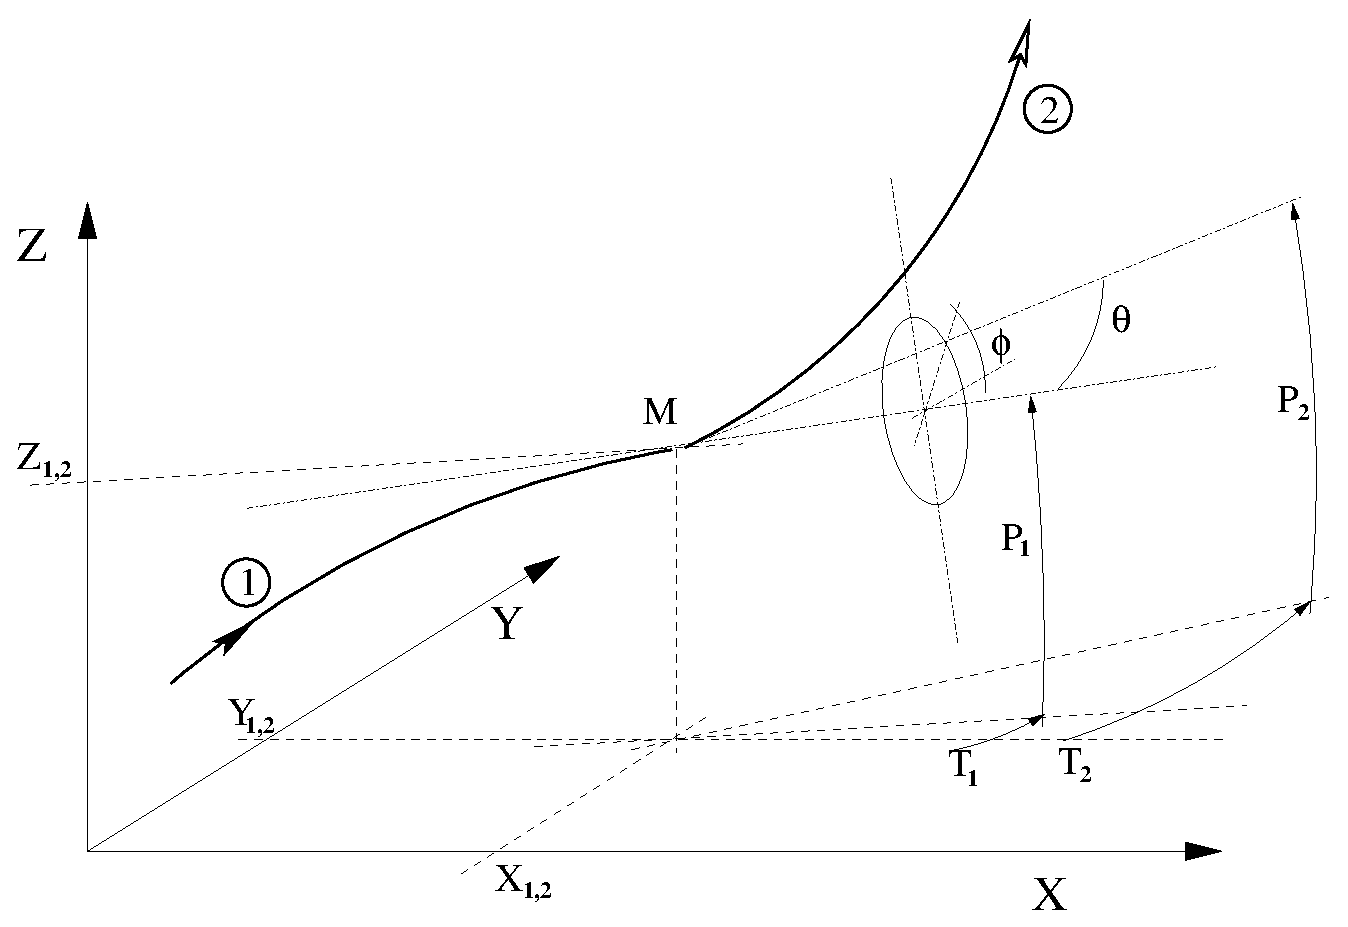
\includegraphics[width=14cm]{Fig6.eps}}
}
{\setlength{\captionwidth}{15cm}
\hangcaption[Fig6]{\label{fig6}%
At position $ M(X_1,Y_1,Z_1) $, particle~1 decays into 2 and 3~; \zgou\ then calculates the trajectory of~2, while 
3 is discarded. \\ 
$\theta$ and $\phi$ are the scattering angles of particle 2 relative to the 
direction of  the incoming particle 1~; they transform to $ T_2 $ and $ P_2 $ 
in \zgou\ frame.}       }
\end{figure}

\noindent In   \textsl{ESL\index{ESL}}   and  \textsl{CHANGREF\index{CHANGREF}},  
$ F(6,I) $ is compared to $ s $ at the
end of the element. If the decay occurs inside the element, the particle is considered as having 
decayed at its actual limit path length $ s$,  and its coordinates 
at $ s $ are recalculated by translation.  
\bigskip

\noindent The limit path length of all particles  ($I=1$, \IMAX\index{IMAX@{\IMAX}})   is stored in
the array  \textsl{FDES}$(6,I)$, for further statistical purposes. For the same purpose 
(e.g., use of \textsl{HISTO\index{HISTO}}), any particle of type~2 (resulting from decay of~1) 
will be tagged with an $ S $ standing for ``secondary''. When a particle decays, 
its coordinates $ D$, $Y$, $T$, $Z$, $P $ at the decay point are stored in  
\textsl{FDES}$(J,I)$, \mbox{$ J=1,\, 5$}.  
\bigskip

\noindent  NOTE on negative drifts~: \\
The use  of  negative  drifts  with  \textsl{MCDESINT\index{MCDESINT}}  is  allowed 
and correct. 
For instance,  negative drifts  may  occur  in  a  structure   for 
some  of  the  particles  when  using  \CHANGREF\index{CHANGREF} (due to  the  $ Z$-axis 
rotation  or  negative  \textsl{XCE)},  or  when  using  \textsl{DRIFT}  with 
$\XL<0$. 
Provision  has  been  made  to  take  it  into  account during  the \textsl{MCDESINT\index{MCDESINT}}
 procedure,  as follows. 

\noindent If, due   to  a  negative  drift,   a  secondary  particle  reaches 
back the  decay spot of the  primary  particle  from which it originated, then 
that  primary  particle  is  regenerated  with its original coordinates 
at  that  spot. Then   the   secondary   particle   is   discarded   while 
ray-tracing  resumes  in  a  regular way  for the primary  particle which  
is again susceptible of decay  at  the  same  time-of-flight. This  procedure  is made 
possible  by  prior storage  of  the  coordinates of the primary 
particles (in array \textsl{FDES}$(J,I)$) each  time  a  decay  occurs. 

\noindent Negative steps\index{integration step size!negative}\index{XPAS!negative} (\textsl{XPAS}$<0$) in
optical elements are not compatible with  \textsl{MCDESINT\index{MCDESINT}}.  
 \newpage

\subsubsection*{ORDRE~: \ORDRETitl } \label{ORDRE} \index{ORDRE}
\medskip

 The position $ \vec  R $ and velocity $ \vec  u $ of a particle are
obtained from Taylor expansions as described in eq.~(\ref{eq2-2-4}). By default, these 
expansions are up to the fourth order derivative of $ \vec  u$, 

\begin{align*}
	\vec  R_1 
	     & \approx  \vec  R_0 + \vec  u_0 \Delta s +...+ \vec u^{(4)}_0 \, \dfrac{\Delta s^5 }{ 5!} \\
	\vec  u_1 
	     & \approx  \vec  u_0 + \vec  u^{\,\prime}_0 \Delta s  
	        + \ldots + \vec  u^{(4)}_0\, \dfrac{\Delta s^4 }{ 4!}   
\end{align*}
%
 which corresponds to third order derivatives of $ \vec  B $, since (eq.~(\ref{eq2-2-6}))
 
 $$ 
 \vec  u^{(4)} = \vec  u^{\,\prime\prime\prime}  \times  \vec  B 
 + 3\vec u^{\,\prime\prime}  \times  \vec  B^{\,\prime}  
 + 3\vec  u^{\,\prime}  \times \vec  B^{\,\prime\prime}  
 + \vec  u  \times   \vec  B^{\,\prime\prime\prime}
$$
%
 and to the third order derivatives of $ \vec  E $ (eq.~(\ref{eq2-2-10})) as well.

However  $ \vec  B^{\,\prime\prime\prime} $,  
or $ \vec  E^{\,\prime\prime\prime} $, and higher order derivatives  may be zero in second order type
optical elements, for instance in a sharp edge quadrupole. Also, in 
several elements, no more than  first and second order field 
derivatives  are implemented in the code.  One may also wish to fasten calculations by 
limiting the time-consuming calculation of lengthy (while possibly ineffective in terms 
of accuracy) Taylor expansions. 

\bigskip

\noindent In that spirit, the purpose of \textsl{ORDRE}, option $ IO=2-5$,  is to allow for 
expansions  to the  $ \vec  u^{(IO)}_0$ term  in eq.~\ref{eq2-2-4}. Default functionning 
is $IO=4$.

\bigskip

\noindent Note the following~: 

As concerns the optical elements
\begin{center}
	\textsl{QUADRUPO, SEXTUPOL, OCTUPOLE, DECAPOLE, DODECAPO,
	MULTIPOL, ELMULT, EBMULT}\index{QUADRUPO}\index{SEXTUPOL}\index{OCTUPOLE}
	\index{DECAPOLE}\index{DODECAPO}\index{MULTIPOL}\index{ELMULT}\index{EBMULT} 
\end{center}
 magnetic field derivatives (see eq.~\ref{eq2-2-7}) have been installed in the code according 
to $ \vec  u^{(5)}_0$ developement order~; it may not 
be as complete for some other optical elements, as well as for the 
 possible electric field  component whose field derivatives may not be provided 
 to more than second order. 

In electric optical elements field  derivatives (eq.~\ref{eq2-2-12}) are usually provided to no more than second 
order, which justifies saving computing time by not pushing Taylor expansions as high as  
$ \vec  u^{(5)}_0$. 


\bigskip

\noindent\textbf{NOTE}~: see also the option \textsl{IORDRE\index{IORDRE}} in field map
declarations (\textsl{DIPOLE-M, TOSCA\index{TOSCA}}, etc.).  
 \newpage

\subsubsection*{PARTICUL~: \PARTICULTitl}  \label{PARTICUL} \index{PARTICUL}

\textsl{PARTICUL} allows the definition of several characteristics of the particles 
(mass, charge, gyromagnetic factor and life-time in the 
center of mass), that are needed in various  procedures as, 
\bigskip           

\begin{tabular}{>{\sl}l!{~:}l}
  MCDESINT  & mass,  COM  life-time\\
  SPNTRK    & mass,  gyromagnetic factor \\
  SRLOSS    & mass, charge \\
  SYNRAD    & mass, charge \\
  Electric and Electro-Magnetic elements
            & mass, charge 
\end{tabular}
\bigskip           

\noindent The declaration of \textsl{PARTICUL} must \textbf{precede} these keywords. 

\noindent
The charge is needed for computing energy gain in electric fields.
The mass is needed for computing time of flight.  If \textsl{PARTICUL} is not
used, the charge defaults to $+e$ and the mass defaults to zero.

\noindent
\textsl{PARTICUL} sets a reference charge annd mass, but individual paritles
have charges and masses as well.  The reference charge relates $B\rho$
to the particle momentum ($B\rho=p/q$); the particle charge relates
the fields ($\vec b$ and $\vec e$) to the scaled fields
($\vec B=\vec b/(B\rho)$ and $\vec E=\vec e/(B\rho)$).

\noindent
Most object definitions assign each particle the reference charge and
mass (cases where they do not are documented).  In cases where the
reference charge and mass have been assigned to a particle, \textsl{PARTICUL}
will change the particle charge and mass to the new reference charge
and mass.  For the few objects where each particle was assigned its
own mass and charge, \textsl{PARTICUL} will not affect those values.  In most
cases (where all particles have the reference charge), the charge
assigned by \textsl{PARTICUL} will not affect the results for systems having
only magnetic fields.

 \newpage

\subsubsection*{REBELOTE~: \REBELOTETitl} \label{REBELOTE} 
\index{REBELOTE}\index{multiparticle}\index{multiturn\index{multiturn} tracking}\index{acceleration}
\index{synchrotron motion}

When \REBELOTE\ is encountered in the input data file, the code execution jumps, 

- either back to the beginning of the data file - the default behavior,  

- or back to a particular \LABEL\ - upon request, 

\noindent and then  a new pass starts, and so on  \textsl{NPASS+1}\index{NPASS} times. 

\noindent The last pass normally ends, as the previous ones, at \REBELOTE, however it may be ended, 
upon request,  at a particular 
\LABEL\ placed at arbitrary location upstream of \REBELOTE. In both cases, the execution 
 is carried on from the keyword which follows \REBELOTE. 

\bigskip

\noindent \REBELOTE\ can be used for Monte Carlo\index{Monte Carlo} simulations when more 
than \IMAX\ particles\index{IMAX@{\IMAX}} are to be tracked. 
In this case, when the following random procedures 
are used~: \textsl{MCOBJET\index{MCOBJET}, OBJETA\index{OBJETA}, MCDESINT\index{MCDESINT}, 
SPNTRK\index{SPNTRK}} \mbox{(\textsl{KSO} = 5)},
their random seeds are not reset and  independent statistics will add up. 

\bigskip

\noindent \REBELOTE\ can be used for  multi-turn tracking in circular machines (e.g.~Synchrotron 
accelerators, FFAGs, etc.).  


\bigskip

\noindent\textbf{Monte Carlo simulations}~: normally $ K=0$.  \textsl{NPASS}\index{NPASS} runs
through the same structure will follow, resulting in the calculation of 
$(1+\text{\textsl{NPASS}})  \ast  \text{\IMAX}$ trajectories.  
\bigskip

\noindent\textbf{Circular machines}~: normally $ K=99$.  \textsl{NPASS} turns in
the same structure will follow, resulting in the tracking of \IMAX\ 
particles over $1+\text{\textsl{NPASS}}$ turns (Note~: for the simulation of 
accelerators and synchrotron motion, see \textsl{SCALING}). 
\bigskip

\noindent Output prints over \textsl{NPASS} runs might result in a
prohibitively big zgoubi.res file. They may be switched on/off  by means of the option 
\mbox{\textsl{KWRIT}$= i.j$}, with $i=1/0$ respectively. The $j$ flag commands printing 
pass numbers  onto the video output, every $10^{j-1}$ turns if $j>0$~; output is switched  
off if $j=0$. 

  
\bigskip

\noindent\REBELOTE\ also provides informations~: statistical calculations and related 
data on particle decay \textsl{(MCDESINT\index{MCDESINT})}, spin tracking\index{spin tracking}  
\textsl{(SPNTRK\index{SPNTRK})}, stopped particles\index{stopped particles} (\textsl{CHAMBR\index{CHAMBR},
 COLLIMA\index{COLLIMA}}), etc.  




 \newpage

\subsubsection*{RESET~: \RESETTitl}  \label{RESET} \index{RESET}

 Piling up problems in \zgou\ input data file is allowed, with 
normally no particular precaution, except that each new problem 
must begin with a new object definition (with \textsl{MCOBJET\index{MCOBJET}, OBJET\index{OBJET}}, 
etc.). Nevertheless, when calling upon certain keywords, flags, 
counters or integrating procedures are involved. 
It may therefore be necessary to reset them. This is the purpose 
of \textsl{RESET\index{RESET}} which normally appears right after the object definition 
and causes each problem to be treated as a new and 
independent one.  
\bigskip

\noindent The keywords or procedures of concern and the effect of 
\textsl{RESET} are the following 
\bigskip

\begin{tabular}{>{\sl}l!{~:}p{13cm}}
  CHAMBR 
       & \textsl{NOUT} = number of stopped particles\index{stopped particles} = 0~;  \textsl{CHAMBR} option  switched  off \\
  COLLIMA 
       & \textsl{NOUT} = number of stopped particles\index{stopped particles} = 0\\
  HISTO 
       &  Histograms are emptied\\
  INTEG 
       & \textsl{NRJ} = number of particles out of range = 0 (\textsl{INTEG} is the numerical 
           integration subroutine~; \textsl{NRJ} is incremented when a particle 
            goes out of a field map)\\
   MCDESINT 
       & Decay in flight option switched off \\
  SCALING 
       &  Scaling options disabled\\
  SPNTRK 
       & Spin tracking option switched off
\end{tabular}
 \newpage

\subsubsection*{SCALING~: \SCALINGTitl} \label{SCALING} \index{SCALING} 
\index{synchrotron motion}

\textsl{SCALING} acts as a function generator dedicated to varying 
fields in optical elements, or potentials in 
electrostatic devices, or  frequency in \textsl{CAVITE\index{CAVITE}}. It is normally intended
to be declared right after the object definition, and used in conjunction 
with \textsl{REBELOTE\index{REBELOTE}}, for the simulation of multiturn\index{multiturn} tracking - possibly including  acceleration
\index{acceleration} cycles.  

\bigskip

\noindent\textsl{SCALING} acts on families of elements,  a family being
designated by its name that  coincides with 
the keyword of the corresponding element. For instance, declaring \textsl{MULTIPOL\index{MULTIPOL}} 
as to be varied will result in the same timing law being applied to all 
\textsl{MULTIPOL\index{MULTIPOL}}'s in the \zgou\ optical structure data file. Subsets can be selected by 
labeling keywords in the data file (section~\ref{sec4.6.8}, page~\pageref{sec4.6.8}) 
and adding the corresponding \LABEL('s)\index{LABEL@{\LABEL}} 
in the \textsl{SCALING} declarations (two \LABEL's maximum). The family name of concern, 
as well as the field versus timing scaling law of that 
family (or frequency versus timing in the case of \textsl{CAVITE\index{CAVITE}}) are given as
input data to the keyword \textsl{SCALING\index{SCALING}}. Up to $NF = 9$ families can be declared
as subject to a scaling law~; a scaling law can be made of up to $NT = 10$~successive timings~; 
between two successive timings, the variation law is linear.  
\bigskip

\noindent An example of data formatting is given in the following. 

\bigskip

{\renewcommand{\arraystretch}{1}
\noindent\begin{tabular}{lll}
  \textsl{SCALING}    &          & - Scaling \\
  1    ~~~~ 4         &          &  Active. $NF = 4$ families of elements are concerned, as listed below \\
  \textsl{QUADRUPO} \textsl{QFA} \textsl{QFB}&          & - Quadrupoles labeled 'QFA' and Quadrupoles labeled 'QFB' \\
  2                   &          & $NT = 2$ timings  \\
  18131.E-3           & 24176.E-3 \qquad 
                                 &   The field increases (linearly) from 18131E-3$\ast B_0 $ 
                                 to 24176E-3$\ast B_0 $  \\
  1                   & 6379     &  from turn 1 to turn 6379\\
  \textsl{MULTIPOL} \textsl{QDA} \textsl{QDB}&          &- Multipoles labeled 'QDA' and Multipoles labeled 'QDB'\\
  2   \\                      
  18131.E-3           &24176.E-3 &  Fields  increase from 18131E-3$\ast {B_i} $ to 
                                  24176E-3$\ast  {B_i} $  ($\forall i=1,\,10$ poles) \\
  1                   & 6379     & from turn 1 to turn 6379\\
  \textsl{BEND}       &          &- All \textsl{BEND}'s (regardless of any \LABEL) \\
  2    \\
  18131.E-3           &24176.E-3 &  Same scaling \\
  1                   & 6379  \\
  \textsl{CAVITE}     &          &- Accelerating cavity \\
  2  \\
  1 ~~~~~ 1.22        &1.33352   &The synchronous rigidity $(\Br )_s $ increases, \\
  1 ~~~~~   1200      & 6379     &from $ (\Br )_{s_o} $ to 1.22 $\ast (\Br)_{s_o} $ from turn 1 to 1200, and \\
                      &          &from 1.22 $\ast (\Br)_{s_o} $ to 1.33352 $ (\Br )_{s_o} $ from turn 1200 to 6379 
\end{tabular} }                   
 \bigskip

\noindent The timing is in unit of turns. In this example, TIMING = 1 to 6379 
(turns). Therefore, at turn number $ N$, $B $ and $ B_i $ are updated in the 
following way. Let \textsl{SCALE}(\textsl{TIMING} $ = N$) be the updating scale factor

\begin{align*}
   \text{SCALE}(N) & = 18.131 \dfrac{24.176-18.131 }{ 1+6379-1} (N-1)  \\
\intertext{and then}
     B(N)   &  = \text{\textsl{SCALE}}(N)B_0 \\ 
     B_i(N) &  = \text{\textsl{SCALE}}(N){B_i}_0 \\
\intertext{The  R.F. frequency is computed using}
     f_{RF} & = \dfrac{hc }{\mathcal{L}} \, 
              \dfrac{q(\Br )_s }{ (q^2(\Br )^2_s + (Mc^2)^2)^{1/2}} 
\end{align*}
%
where the rigidity is updated in the following way. Let $ (\Br)_{s_o} $ be the 
initial rigidity (namely, $ (\Br )_{s_o}= $ \BORO as defined in the keyword
\textsl{OBJET} for instance). Then, at turn number $ N$,   

\begin{alignat*}{2}
	\text{if  }   1 & \leq N\leq 1200 \,          
	            & \text{  then,  \textsl{SCALE}}(N)  & =1+ \dfrac{1.22-1 }{ 1+1200-1}\, (N-1) \\
	\text{if  }   1200 & \leq N\leq 6379 \,           
	            & \text{  then,  \textsl{SCALE}}(N)  & =1.22+ \dfrac{1.33352-1.22 }{ 1+6379-1200}\,(N-1200)    
\end{alignat*}
 
 \noindent and then,

$$ (\Br )_s(N) = \text{\textsl{SCALE}}(N)\cdot (\Br )_{s_o} $$
%
from which value the calculations of $ f_{RF}(N) $ follow. 


\bigskip

 \noindent $NT$ can take negative values, then acting as an option switch (rather than giving number of timings), as follows~: 

$\bullet ~ NT = -1$~: this is convenient for synchrotron acceleration using trivial RF law $f_{RF} = h/T_{rev}$. In this case 
the next two lines both contain a single data (as for $NT=1$), respectively the starting scaling factor value, and 1.  
The current field scaling factor can then be updated (computed) 
 from the energy kick by the cavity if for instance \textsl{CAVITE/IOPT=2} is used. 

$\bullet ~ NT = -2$~: this is convenient for reading an RF law for \textsl{CAVITE} from an external data file, 
including usage for acceleration in fixed field accelerators. To be documented. 


\bigskip

\noindent {\bf Note~:} It may happen that some optical elements won't scale, for source code developement reasons. 
This should be paid attention to. 



\newpage

\subsubsection*{SPNTRK~: \SPNTRKTitl} \label{SPNTRK} \index{SPNTRK|textbf}
\medskip

The keyword \textsl{SPNTRK} permits switching on the spin tracking\index{spin tracking} 
option. It also permits the attribution of an initial spin component to each one of the 
\IMAX\index{IMAX@{\IMAX}} particles of the beam, following a distribution that depends 
on the option index \textsl{KSO}. It must be preceded by \textsl{PARTICUL\index{PARTICUL}} for
the definition of  mass and gyromagnetic factor.  
\medskip

\noindent\textbf{KSO = 1  (respectively 2, 3)~:} the \IMAX\ particles
of the beam are given a longitudinal (1,0,0) spin component (respectively 
transverse horizontal (0,1,0), vertical (0,0,1)).  
\medskip

\noindent\textbf{KSO = 4~:} initial spin components are entered explicitly for
each one of the \IMAX\index{IMAX@{\IMAX}} particles of the beam.  
\medskip

\noindent\textbf{KSO = 4.1~:} three initial spin components $S_X, S_Yn S_Z$ are entered explicitly just once, 
they are then assigned to  each one of the \IMAX\index{IMAX@{\IMAX}} particles of the beam.  
\medskip

\noindent\textbf{KSO = 5~:} random generation of \IMAX\index{IMAX@{\IMAX}} initial spin
conditions as described in Fig.~\ref{fig7}.  
Given a mean polarization axis (S) defined by its angles $ T_0 $ and $ P_0 $, 
and a cone of angle~A with respect to this axis, the \IMAX\index{IMAX@{\IMAX}} spins are sorted randomly in a 
Gaussian distribution

$$ p(a) = \exp \left[- \frac{(A-a)^2 }{ 2\delta A^2} \right]/ \delta A\,  \sqrt{2\pi}   $$
%
and within a cylindrical uniform distribution around the (S) 
axis. Examples of simple distributions available by this mean are 
given in Fig.~\ref{fig8}.  


%%%%%%%%%%%%%%figure%%%%%%%%%%%%%%
\begin{figure}[H]
%\vspace{11 truecm}
%%%Figure 7
\centerline{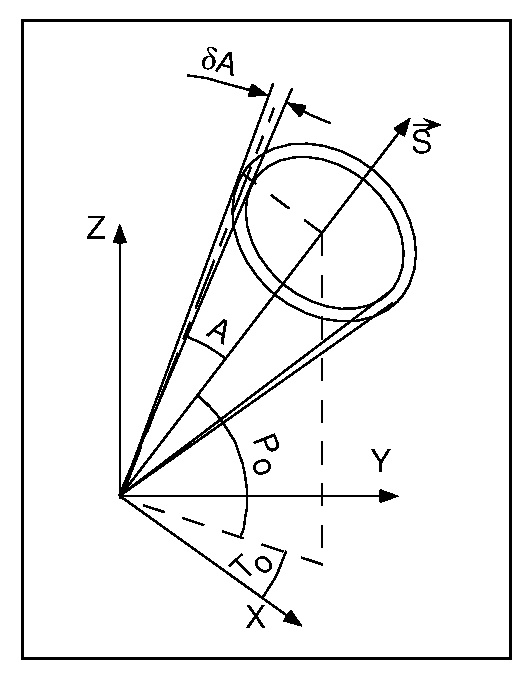
\includegraphics[height=10cm]{Fig7.ps}}
{\setlength{\captionwidth}{15cm}
\hangcaption[Fig7]{\label{fig7}Spin distribution as obtained with option \textsl{KSO} = 5.\\
          The spins are distributed within an annular strip 
         $\delta A$ (standard deviation)  
          at an angle $A$ with respect to the 
         axis of mean polarization (S) defined by $T_0$  and $P_0$.} 
}\end{figure}
%%%%%%%%%%%%%%figure%%%%%%%%%%%%%%
%\figureh 5cm   \figurev 7cm  
\begin{figure}[H]
%\vspace{8.5 truecm}
%%%Figure 8
\centerline{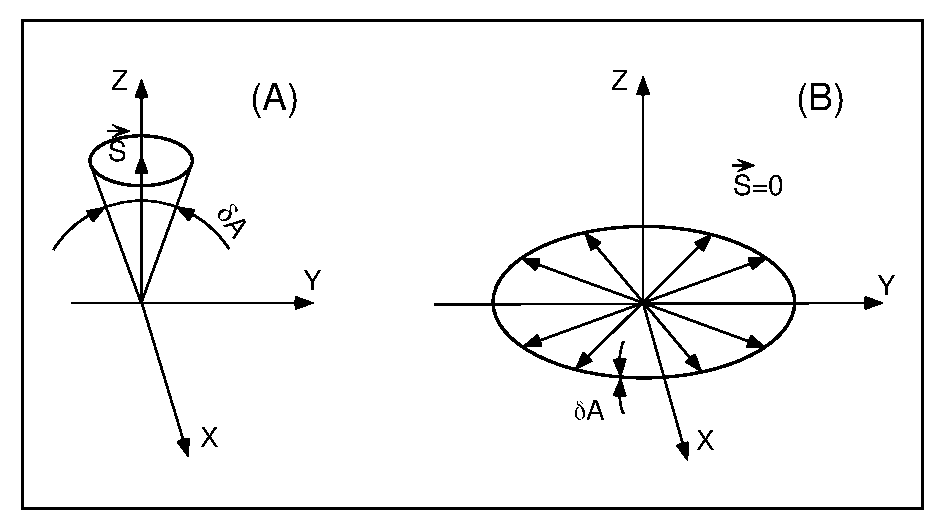
\includegraphics[width=15cm]{Fig8.ps}}
{\setlength{\captionwidth}{14cm}
\hangcaption[Fig8]{\label{fig8}Examples of the use of	\textsl{KSO} =5. \\
A~: Gaussian	distribution around	a mean vertical	polarization axis, 
 obtained   with	$T_0$  = arbitrary,	$P_0 = \pi /2$,	$A = 0$ and $\delta A \not=  0$.\\
B~: Isotropic distribution in the median	plane, obtained	with 
 $P_0 =	\pm	 \pi /2$, 
$A = \pi /2$,	and	$\delta	A =	0$.} }
 \end{figure}
\newpage

\subsubsection*{SRLOSS~: \SRLOSSTitl\ } \index{SRLOSS|textbf}\label{SRLOSS}
\index{synchrotron radiation loss}\cite{FMSEA-00-01}

\noindent The keyword \textsl{SRLOSS} allows activating or stopping (option $KSR=1,0$ respectively) 
 stepwise tracking  of energy loss by emission of 
photons in magnetic fields and the ensuing particle energy perturbation. It must be
preceded by \textsl{PARTICUL}\index{PARTICUL} for defining  mass and charge values as they enter in the 
definition of SR parameters. 


\bigskip

Statistics on SR parameters are perform while tracking, results of which can be obtained by means of keyword 
 SRPRNL. 


\newpage

\subsubsection*{SYNRAD~: \SYNRADTitl}\label{SYNRAD}\index{SYNRAD|textbf}\index{synchrotron radiation spectra}

\noindent The keyword \textsl{SYNRAD} enables (or disables) the calculation of 
synchrotron radiation (SR) electric field and spectral angular energy density. It must be 
preceded by \textsl{PARTICUL}\index{PARTICUL} for defining  mass and charge values, as they enter 
in the definition of SR parameters. 

\bigskip

\noindent\textsl{SYNRAD} is supposed to appear a first time at the 
location where SR~calculations should start, with the first data \textsl{KSR} set 
to~1. It results in on-line storage of the electric field vector and 
other relevant quantities in zgoubi.sre\index{zgoubi.sre}, as step by step integration 
proceeds. The observer position ($XO$, $YO$, $ZO$) is specified next 
to \textsl{KSR}.
\bigskip

\noindent Data stored in zgoubi.sre~:
 
 \begin{tabular}{l} 
 ($ELx$, $ELy$, $ELz$)~:  electric field vector $\vec\Ecal $ 
 						(eq.~\ref{eqN4.1}) \\
 $(btx, bty, btz) = \vec\beta= \dfrac{1}{c} \times$ particle velocity \\
$(gx, gy, gz) = \dfrac{d\vec\beta}{dt} =$ particle acceleration (eq.~\ref{eqN4.3}) \\					
$\Delta \tau =$ observer time increment (eq.~\ref{eqN4.2}) \\
$t' = \tau  - r(t')/c = $ retarded (particle) time \\
$(rtx, rty, rtz)~: \vec R(t)$, particle to observer vector (eq.~\ref{eqN4.4}) \\
$(x, y, z) =$ particle coordinates\\
$\Delta s = $ step size in the magnet (fig. 2)\\
$NS=$ step number\\
$I=$ particle number\\
$LET(I)=$ tagging letter\\
$IEX(I)\index{IEX@{\IEX}}=$ stop flag (see section~\ref{sec4.6.6}) 
\end{tabular}
\bigskip


\noindent\textsl{SYNRAD} is supposed to appear a second time at the 
location where SR~calculations should stop, with \textsl{KSR} set 
to~2. It results in the output of the angular energy density 
$\int_{\nu_1}^{\nu_2} \partial^3 W / \partial \phi \, \partial \psi 
\, \partial \nu$ (eq.~\ref{eqN4.11}) as calculated from the Fourier transform 
of the electric field (eq.~\ref{eqN4.11}). The spectral range of 
interest and frequency sampling ($\nu_1$, $\nu_2$, $N$) are specified 
next to \textsl{KSR}.
\bigskip

\noindent Note that \textsl{KSR} = 0 followed by a dummy line of 
data allows temporary inhibition of SR~procedures.

\newpage

\subsection{Optical Elements and related numerical procedures} \label{sec4.4}

\subsubsection*{AIMANT~:  \AIMANTTitl}\label{AIMANT}\index{AIMANT|textbf}
\medskip

The keyword \textsl{AIMANT} provides an automatic
generation of a dipole median plane field map in polar coordinates. A more recent and improved version will be 
found in \textsl{DIPOLE-M\index{DIPOLE-M}}. The extent of the map is defined by the 
following parameters, as shown in Figs.~\ref{fig9}A and~\ref{fig9}B. 

 \begin{tabular}{>{\sl}l!{~:}l}
	 AT &  total angular aperture\\
	 RM & mean radius used for the positioning of field boundaries\\
	 RMIN, RMAX
	    &  minimum and maximum radial boundaries of the map 
 \end{tabular}
\bigskip

\noindent The 2 or 3 effective field boundaries (EFB) inside the map are
defined from  geometric boundaries, the shape and position of which are determined by the 
following parameters.  


\begin{tabular}{l!{~:}l}
	 \textsl{ACENT} 
	    & arbitrary  angle, used for the positioning of the EFB's. \\
	$\omega$ &  azimuth of an EFB with respect to  \textsl{ACENT}\\
	$\theta$ & angle of a boundary with respect to its azimuth (wedge angle)\\ 
	$R_1$, $R_2$  &  radius of curvature of an EFB\\
	$U_1$, $U_2$  &  extent of the linear part of the EFB. 
\end{tabular}
\bigskip

\noindent At  any node  of the map mesh, the value of the $Z$ 
component of the field is calculated as 

 \begin{equation}
	 B_Z =  \mathcal{F} \ast  B_0 \ast  
	      \left(1+N \ast  
	           \left( \frac{R-RM }{ RM}\right) 
	           + B \ast  \left(\frac{R-RM }{ RM} \right)^2 
	           + G \ast  \left(\frac{R-RM }{ RM} \right)^3 
	      \right) 
 	\label{eq4-4-1}
 \end{equation}
%
 where  $ N$, $B $ and $ G $ are  respectively  the first, second and
third order field indices and $ \mathcal{F}$ is the fringe field 
coefficient. 


\subsubsection*{Calculation of the Fringe Field Coefficient} 

With  each EFB a realistic extent of the fringe field, $\lambda$, 
is associated (Figs.~\ref{fig9}A and~\ref{fig9}B),  
and a fringe field coefficient $ F$ is 
calculated. In the following $\lambda$ stands for either $ \lambda_ E $
(Entrance), $ \lambda_ S $ (Exit) or $ \lambda_ L $ (Lateral EFB). 
 
\noindent If a node of the map mesh is at a distance of the EFB larger than
$\lambda$, then $ F=0 $ outside the field map and $ \mathcal{F}=1 $ inside.  
If a node is inside the fringe field zone, then $  F$   is calculated as follows. 

\noindent Two options are available, for the calculation of $ F$, depending
on the value of $\xi$. 

\noindent\textbf{If } $\mathbf{\xi  \geq 0}$, $ F $ is a  second
order type fringe field (Fig.~\ref{fig11}) given by 


\begin{gather}
		F  = \dfrac{1 }{ 2} \, \dfrac{(\lambda -s)^2 }{ \lambda^2-\xi^ 2} \quad 
		         ~~ \text{if }~   \xi  \leq  s \leq \lambda  \\
		F  = 1- \dfrac{1 }{ 2} \, \dfrac{(\lambda -s)^2 }{ \lambda^2-\xi^ 2}\quad 
		        ~~ \text{if }~   -\lambda  \leq  s \leq  -\xi 
\end{gather}
where $ s $ is the distance to the EFB, and
\begin{gather}
		 F  = \dfrac{1 }{ 2} + \dfrac{s }{ \lambda +\xi} \quad
		         ~~ \text{if }~  0 \leq  s \leq  \xi  \\
	    F   = \dfrac{1 }{ 2} - \dfrac{s }{ \lambda +\xi}\quad  
		       ~~ \text{if }~   -\xi  \leq  s \leq  0  
\end{gather}
 
\noindent This simple model allows a rapid calculation of the fringe field,
but may lead to erratic behavior of the field when extrapolating out of the median plane, 
due to the discontinuity of $ d^2B/ds^2 $ at $ s=\pm \xi $ and $ s=\pm \lambda $. 
For more accuracy it is better to use the next option. 

\newpage
%%%%%%%%%%%%%%figure%%%%%%%%%%%%%%
\begin{figure}[H]
%\vspace{21 truecm}
%%%Figure 9
\centering
            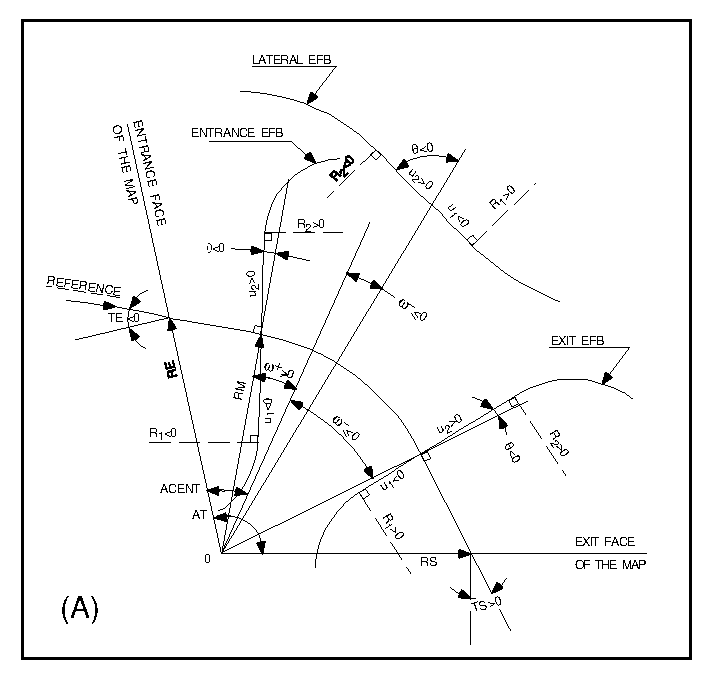
\includegraphics[width=12cm]{Fig9a.eps}
            \vfill
            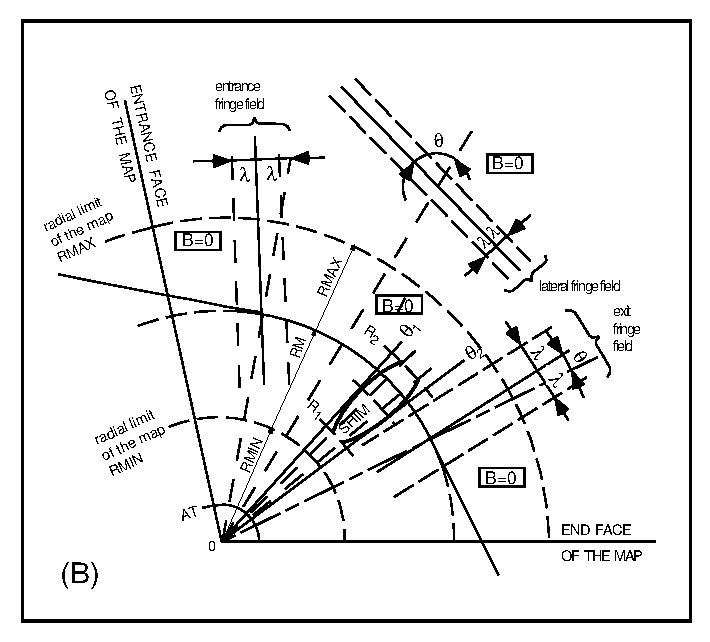
\includegraphics[width=12cm]{Fig9b.eps}
\hangcaption[Fig9]{\label{fig9} A~: Parameters used to define the field map and 
geometric boundaries. \\
  B~: Parameters used to define the field map and fringe fields.}  
\end{figure}  
\newpage

\noindent\textbf{If $\mathbf{\xi  = -1}$},  $ F $ is an exponential type
fringe field (Fig.~\ref{fig11}) given by~\cite{Biblio12}  %%%   [12]

 \begin{gather}
	 F = \dfrac{1 }{ 1+ \exp  P(s)}
 	\label{eq4-4-4} \\
\intertext{where $ s $ is the distance to the EFB, and }
    P(s) = C_0
       +C_1 \left(  \dfrac{s }{ \lambda} \right) 
       +C_2 \left( \dfrac{s }{ \lambda} \right)^2 
       + C_3 \left( \dfrac{s }{ \lambda} \right)^3 
       +C_4 \left( \dfrac{s }{ \lambda} \right)^4 
       + C_5 \left(\dfrac{s }{ \lambda} \right)^5 \label{eq4-4-5}
\end{gather}
%
The values of the coefficients $ C_0 $ to $ C_5 $ should be such that the 
derivatives of $ B_Z$ with respect to $ s $ be negligible at $ s=\pm \lambda $, so as not
to perturb the extrapolation of $ \vec B $ out of the median plane  (this restriction 
no longer holds in the improved version \textsl{DIPOLE-M\index{DIPOLE-M}}).  

\noindent It is also possible to simulate a shift of the EFB, by giving a non
zero value to the parameter \textsl{SHIFT}.  $ s $ is then changed to $ s  -$~\textsl{SHIFT} in the 
previous equation.   This allows small variations of the total 
magnetic length. 

\noindent Let $ F_E $ (respectively $ F_S$, $F_L$)   be the fringe field
coefficient attached to the entrance (respectively exit, lateral) EFB following eqs.\ above. At any
node of the map mesh, the resulting value of the fringe field coefficient (eq.~\ref{eq4-4-1}) is 
(Fig.~\ref{fig12})  

$$ \mathcal{F}= F_E \ast  F_S \ast  F_L $$
%
 ($F_L=1 $ if no lateral EFB is requested). 

\subsubsection*{The Mesh of the Field Map} 

The magnetic field is calculated at the nodes of a mesh with polar
coordinates, in the median plane.  The radial step is given by 
 \begin{align*}
	 \delta R & = \dfrac{\text{\textsl{RMAX - RMIN}} }{\text{\textsl{IRMAX}}-1} \\
\intertext{ and the angular step by} 
	\delta \theta  & = \dfrac{AT }{ \text{\textsl{IAMAX}}-1} 
 \end{align*}
%
\noindent where, \textsl{RMIN} and  \textsl{RMAX}   are the lower and upper
radial limits of the field map, and $ AT $ is its total angular aperture (Fig.~\ref{fig9}B).  
 \textsl{IRMAX} and  \textsl{IAMAX} are the total number of nodes in the radial and 
 angular directions. 
 

 
 \subsubsection*{Simulating Field Defects and Shims } 
 
  Once the initial map is calculated, it is possible to modify it by
means of the parameter \textsl{NBS}, so as to simulate field defects or shims. 
\bigskip

\noindent\textbf{If} $\mathbf{NBS = -2}$, the map is globally modified by a
perturbation proportional to $ R-R_0 $, where $ R_0 $ is an arbitrary radius, 
with an amplitude $ \Delta B_Z/B_0 $, so that $ B_Z $ at the nodes of the mesh is replaced by 

$$ B_Z \ast  \left( 1+ \frac{\Delta B_Z }{ B_0} \,
                 \frac{R-R_0 }{\text{\textsl{RMAX}} - \text{\textsl{RMIN}}} \right) $$


\noindent\textbf{If} $\mathbf{NBS = -1}$, the perturbation is proportional to
$ \theta -\theta_ 0 $, and $ B_Z $ is replaced by 

$$ B_Z \ast  \left(1+ \frac{\Delta B_Z }{ B_0}\, \frac {\theta -\theta_ 0 }{ AT}\right) $$


\newpage

%%%%%%%%%%%%%%figure%%%%%%%%%%%%%%
\begin{figure}[H]
  \centering
%%%Figure 10
  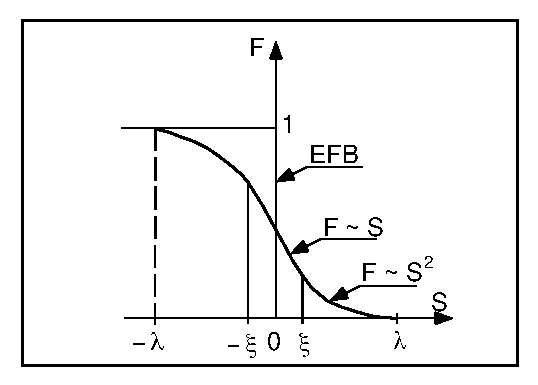
\includegraphics[width=9cm]{Fig10.ps}
  \vfill
%%%Figure 11
  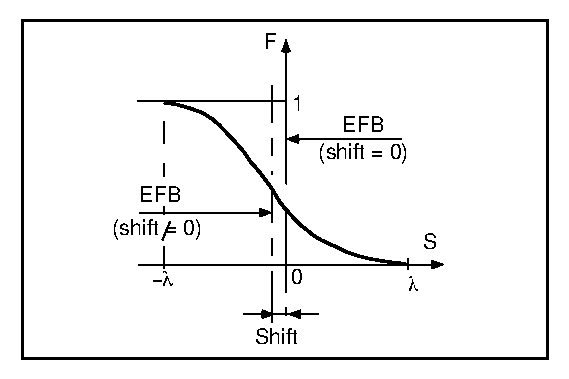
\includegraphics[width=9cm]{Fig11.ps}
{\setlength{\captionwidth}{18cm}
\hangcaption{\label{fig11}Second order type fringe field (upper plot) 
and exponential type fringe field (lower plot).}}
\end{figure}

\vfill
\begin{figure}[H]
%\vspace{10 truecm}
%%%Figure 12
\centerline{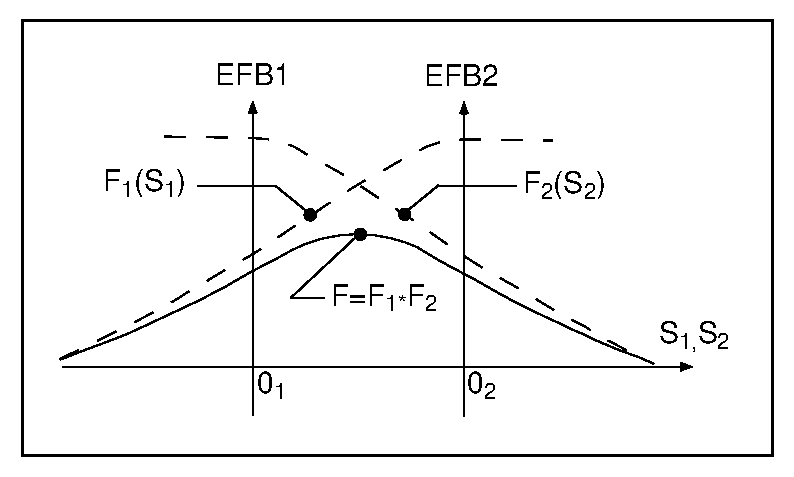
\includegraphics[width=12cm]{Fig12.ps}}
{\setlength{\captionwidth}{15cm}
\hangcaption[Fig12]{\label{fig12} Effective value of $\mathcal{F}$ for overlapping fringe
fields $ F_1 $ and $ F_2 $ centered at $ O_1 $ and $ O_2 $. }}
\end{figure}

\newpage


\noindent\textbf{If } $\mathbf{NBS \geq 1}$, then \textsl{NBS} shims are introduced at
positions $ \dfrac{R_1+R_2 }{ 2}$, $\dfrac{\theta_ 1+\theta_ 2 }{ 2} $  
(Fig.~\ref{fig13})~\cite{Biblio13}  %%    [13]

\noindent The initial field map is modified by shims with second order
profiles given by 

$$ \theta  = \left(\gamma  + \frac{\alpha }{ \mu} \right) 
       \,\beta  \, \frac{X^2 }{\rho^ 2} $$
%
 where $ X $ is shown in  Fig.~\ref{fig13},  
 $ \rho =\dfrac{R_1+R_2 }{ 2}$ is 
the central radius, $\alpha$ and $\gamma$ are the angular limits of the shim, 
$\beta$ and $\mu$ are parameters. 

\noindent At each shim, the value of $ B_Z $ at any node of the initial map is
replaced by 

$$ B_Z \ast  \left(1+F\theta  \ast  FR \ast  \frac{\Delta B_Z }{ B_0} \right)
$$
%
 where $ F\theta =0 $ or $ FR=0 $ outside the shim, and $ F\theta =1$ and $ FR=1 $ inside.  

\subsubsection*{Extrapolation Off Median Plane} 

The vector field $ \vec  B $ and its derivatives in the median plane are 
calculated by means of a second or fourth order polynomial 
interpolation, depending 
on the value of the parameter \textsl{IORDRE\index{IORDRE}} (\textsl{IORDRE}=2, 25 or 4, 
see section~\ref{sec2.4.2}). 
The transformation from polar to Cartesian coordinates is performed 
following eqs.~(\ref{eq2-4-8} or \ref{eq2-4-9}). Extrapolation off median phase is then performed 
by means of Taylor expansions following the procedure described in section~\ref{sec2.3.2}.  


\vfill 

%%%%%%%%%%%%%%figure%%%%%%%%%%%%%%
\begin{figure}[H]
%\vspace{20 truecm}
%%%Figure 13
\centerline{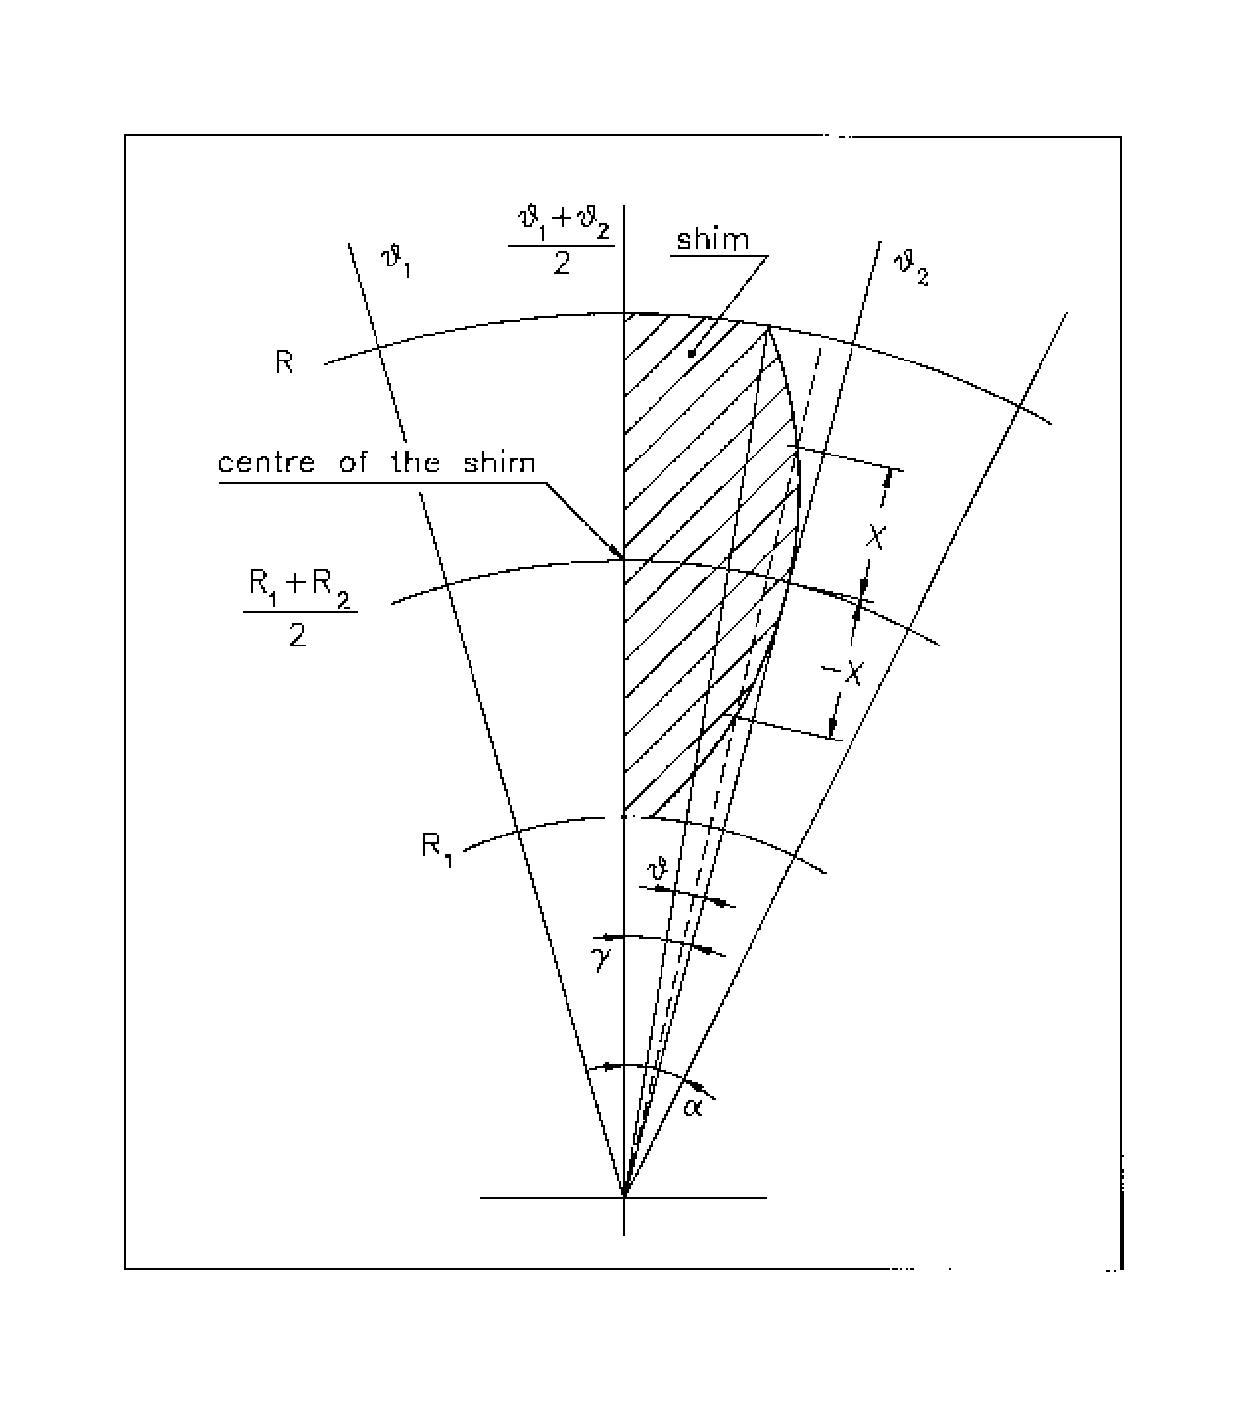
\includegraphics[height=10cm]{Fig13.ps}}
{\setlength{\captionwidth}{14cm}
\hangcaption[Fig13]{\label{fig13}A second order profile shim.  The shim is centered at 
$ \dfrac{(R_1+R_2) }{ 2} $ and $ \dfrac{(\theta_ 1+\theta_ 2) }{ 2} $.}   }
\end{figure}




\newpage

\subsubsection*{AUTOREF~: \AUTOREFTitl}\label{AUTOREF}\index{AUTOREF|textbf} 
\medskip

\textsl{AUTOREF} positions the new reference frame following 3~options~:
\bigskip

\noindent\textbf{If} $\mathbf{I = 1}$, \textsl{AUTOREF} is equivalent to 

$$ \text{\textsl{CHANGREF}} \lbrack XCE=0, YCE=Y(1), ALE=T(1)\rbrack $$
\index{CHANGREF}%
 so that the new reference frame is at the exit of the last element,
with particle~1 at the origin with its horizontal angle set to $ T=0$.   

\bigskip

\noindent\textbf{If} $\mathbf{I=2}$, it is equivalent to

$$ \text{\textsl{CHANGREF}} \lbrack XW, YW, T(1)\rbrack $$
%
 so that the new reference frame is at the position $ (XW, YW) $ of
the waist (calculated automatically in the same way as for 
\textsl{IMAGE\index{IMAGE}}) of the three rays number 1, 4 and 5 (compatible for instance
with \textsl{OBJET\index{OBJET}, KOBJ}  =  5, 6 together with the 
use of \textsl{MATRIX})\index{MATRIX} while $T(1)$ is set to zero.  

\bigskip

\noindent\textbf{If} $\mathbf{I=3}$,  it is equivalent to 

$$\text{\textsl{CHANGREF}} \lbrack XW,YW,T(I1)\rbrack $$
%
 so that the new reference frame is at the position $ (XW, YW) $ of
the waist (calculated automatically in the same way as for 
\textsl{IMAGE}) of the three rays number I1, I2 and I3 specified as data,  while $T(1)$ is set to zero.
 
\newpage


\subsubsection*{BEND~: \BENDTitl}\label{BEND}  \index{BEND|textbf}
\medskip

\textsl{BEND}  is one of the several keywords available for the
simulation of dipole magnets. It presents the interest of easy handling, and is well adapted for 
the simulation of synchrotron dipoles and such other regular dipoles as sector magnets with wedge 
angles. 

\bigskip

\noindent The field in \textsl{BEND}  is defined in a Cartesian coordinate frame (unlike for instance \textsl{DIPOLE[S]} 
that uses a polar frame).  As a consequence, having particle coordinates at entrance  or exit of the magnet 
referring to the  curved  main direction of motion may 
require using \textsl{KPOS}, in particular \textsl{KPOS=3}  (in a circular machine cell for instance). 

\bigskip

\noindent The dipole simulation is performed from the magnet geometrical length $ \XL $, from
 the skew angle (rotation \wrt\ the X axis, useful for obtaining vertical deviation magnet), and from the 
field $ B1 $  such that   in absence of fringe field the deviation $\theta$ satisfies 
$ \XL = 2 \frac{\BORO}{B1} \sin(\frac{\theta}{2})$. 

\bigskip

\noindent Then follows the description of the entrance and exit EFB's and
fringe fields.       The wedge angles $W_E $ 
(entrance) and $W_S $ (exit) are defined with respect to the sector angle, 
with the signs as described in Fig.~\ref{fig14}.  
Within a distance $ \pm X_E(\pm X_S) $ on both sides of the entrance (exit) EFB, 
the fringe field model is used~; elsewhere, the field is supposed to be uniform. 

\bigskip

\noindent If $\lambda_{E} $ (resp. $\lambda_{S} $) is zero sharp edge field model is assumed at entrance 
(resp. exit) of the magnet and $X_E$ (resp. $X_S$) is set to zero.  In this case, the wedge angle vertical first order 
focusing effect (if $\vec  B1$ is non zero) is simulated at magnet entrance and exit by a kick 
$P_2 = P_1 - Z_1 \tan (\epsilon / \rho)$ applied to each particle ($P_1$, $P_2$ are the vertical angles 
upstream and downstream the EFB, $Z_1$ the vertical particle position at the EFB, $\rho$ the local horizontal 
bending radius and $\epsilon$ the wedge angle experienced by the particle~; $\epsilon$ depends on the horizontal angle T).


\bigskip

\noindent Magnet (mis-)alignement is assured by \textsl{KPOS}. 
\textsl{KPOS} also  allows some degrees of automatic alignement useful for periodic structures (section~\ref{sec4.6.2}).

\vfill
%%%%%%%%%%%%%%%figure%%%%%%%%%%%%%%
\begin{figure}[H]
  %\vspace{12 truecm}
  %%%Figure 14
%  \centerline{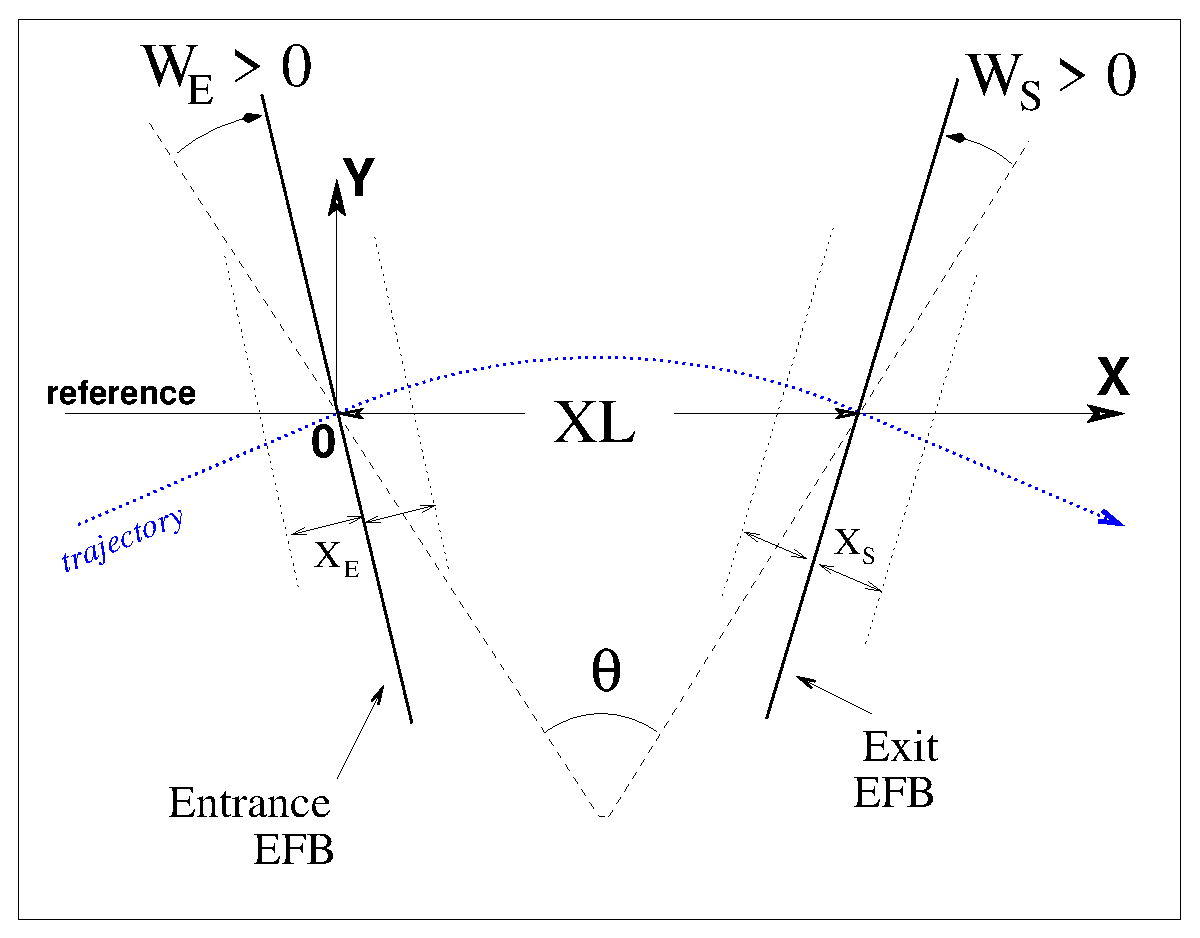
\includegraphics[height=12cm,angle=-90]{Fig14.ps}}
  \centerline{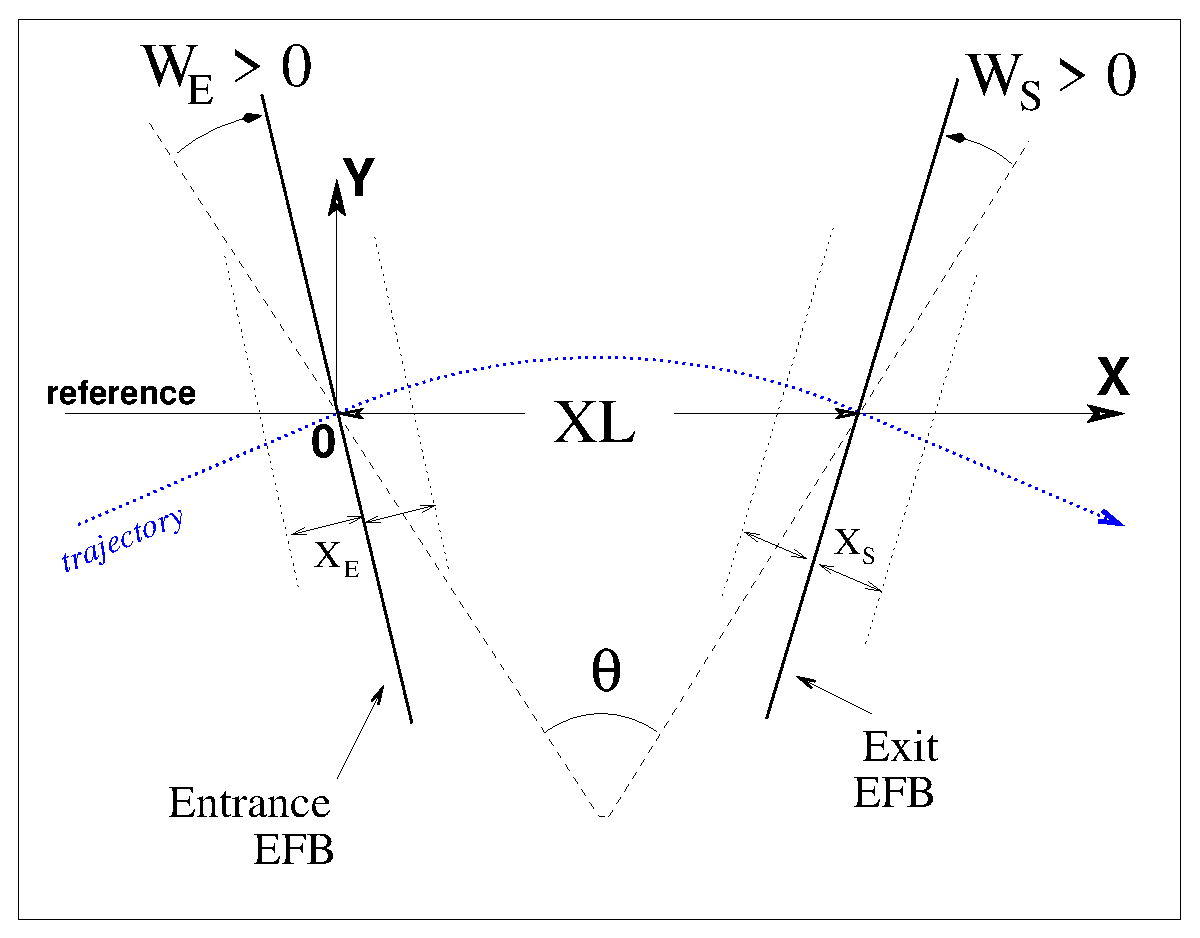
\includegraphics[height=8cm]{Fig14.eps}}
  {\setlength{\captionwidth}{12cm}
	\hangcaption[Fig14]{\label{fig14}
               \CapBEND
    } }
\end{figure}

\vfill
\newpage


\subsubsection*{BREVOL~: \BREVOLTitl} \label{BREVOL}\index{BREVOL|textbf}
\medskip

\textsl{BREVOL}  reads a 1-D axial field map from a storage data file,
whose content must fit the following \FORTRAN reading sequence   
\bigskip


{\footnotesize
\begin{verbatim}
	      OPEN (UNIT = NL, FILE = FNAME, STATUS = `OLD' [,FORM='UNFORMATTED'])
	      DO 1 I = 1, IX
	        IF (BINARY) THEN 
	              READ(NL) X(I), BX(I)
	        ELSE
	              READ(NL,*) X(I), BX(I)
	        ENDIF
	1     CONTINUE
\end{verbatim}}
\medskip

\noindent where $IX$ is the number of nodes along the (symmetry) $X$-axis, $X(I)$
their coordinates, and $BX(I)$ the values of the $X$ component of the field. $BX$ is 
normalized with \textsl{BNORM} factor prior to ray-tracing, as well  X is normalized with 
a  \textsl{XNORM} coefficient (usefull to convert to centimeters, the working units in  \zgoubi). 
For binary files, \textsl{FNAME} must begin with \mbox{`B\_ '} or  \mbox{`b\_ '}, 
a flag `BINARY' will thus be set to `.TRUE.'. 

\bigskip

\noindent $X$-cylindrical symmetry is assumed, resulting in $BY$ and $BZ$ taken to 
be zero on axis. $ \vec {B} {(X,Y,Z)} $ and its derivatives along a
particle trajectory are calculated by means of a 5-point polynomial fit followed by second 
order off-axis Taylor series extrapolation (see sections~\ref{sec2.3.1}, \ref{sec2.4.1}).  
\bigskip

\noindent Entrance and/or exit integration boundaries may be defined in the same way 
as in \textsl{CARTEMES\index{CARTEMES}} by means of the flag $ID$ and coefficients
$A$, $B$, $C$, etc. 

\newpage

\subsubsection*{CARTEMES~: \CARTEMESTitl}\label{CARTEMES}\index{CARTEMES|textbf}
\medskip

\textsl{CARTEMES}  was originally dedicated to the reading 
and processing of
the measured median plane field maps of the QDD spectrometer  SPES2 at Saclay.  However, it can be
used for the reading of any other 2-D median plane maps, provided that the format of the
field data storage file fits the following \FORTRAN sequence 


{\footnotesize
\begin{verbatim}
	      OPEN (UNIT = NL, FILE = FNAME, STATUS = `OLD' [,FORM='UNFORMATTED'])
              IF (BINARY) THEN 
                READ(NL) (Y(J), J=1, JY)
              ELSE
                READ(NL,FMT='(10F8.2)') (Y(J), J=1, JY)
              ENDIF
              DO 1 I=1, IX
	        IF (BINARY) THEN 
	          READ(NL) X(I), (BMES(I,J), J=1, JY)
	        ELSE
	          READ(NL,FMT='(10F8.1)') X(I), (BMES(I,J), J=1, JY) 
                ENDIF
        1     CONTINUE
\end{verbatim}}

\noindent where, $IX$  and $JY$  are the number of longitudinal
and transverse horizontal nodes of the uniform mesh, and $X(I)$, $Y(J)$ their coordinates.  
\textsl{FNAME} 
 is the file containing the field data. For binary files, \textsl{FNAME} must begin with
\mbox{`B\_ '} or \mbox{`b\_'},  a flag `BINARY' will thus be set to `.TRUE.'.  
\bigskip

\noindent The measured field \textsl{BMES} is normalized with \textsl{BNORM},

$$ B(I,J) = \text{\textsl{BMES}}(I,J) \times  \text{\textsl{BNORM}} $$

\noindent As well the longitudinal coordinate  X is normalized with 
a  \textsl{XNORM} coefficient (usefull to convert to centimeters, the working units in  \zgoubi. 

\noindent The vector field, $ \vec  B $, and its derivatives out of the median
plane are calculated by means of a second or fourth order polynomial 
interpolation, depending on 
the value of the parameter \textsl{IORDRE\index{IORDRE}} (\textsl{IORDRE} = 2, 25 or 4, 
see section~\ref{sec2.4.2}). 
\bigskip

\noindent In case a particle  exits the mesh, its \IEX\index{IEX@{\IEX}} flag is set to $-1$ (see section~\ref{sec4.6.6} on 
page~\pageref{sec4.6.6}), however it is still tracked with the field being {\it extrapolated} from 
the closest mesh nodes of the map. Note that such extrapolation process may induce eratic behavior if the distance from the mesh gets 
too large. 

\bigskip

\noindent Entrance and/or exit integration boundaries can be defined with 
the flag $ID$\index{ID@{\textsl{ID}}|textbf}, as follows (Fig.~\ref{fig15}).
\bigskip

\noindent \textbf{If  $\mathbf{ID = 1}$~:} the integration in the field 
is terminated on a boundary with equation $A'X + B'Y + C'=0 $, and 
then the trajectories are extrapolated linearly onto the exit end of the 
map.
\medskip

\noindent \textbf{If  $\mathbf{ID = -1}$~:} an entrance boundary is 
defined, with equation $A'X + B'Y + C'=0 $, up to which  trajectories are 
first extrapolated linearly from the map entrance end, prior to being 
integrated in the field.
\medskip

\noindent \textbf{If  $\mathbf{ID \geq 2}$~:} one entrance boundary, and 
$ID-1$~exit boundaries are defined, as above. The integration in the 
field terminates on the last ($ID - 1$) exit boundary. No extrapolation onto 
the map exit end is performed in this case.

\newpage

%%%%%%%%%%%%%%figure%%%%%%%%%%%%%%
\begin{figure}[H]
%\vspace{19 truecm}
%%%Figure 15
\centerline{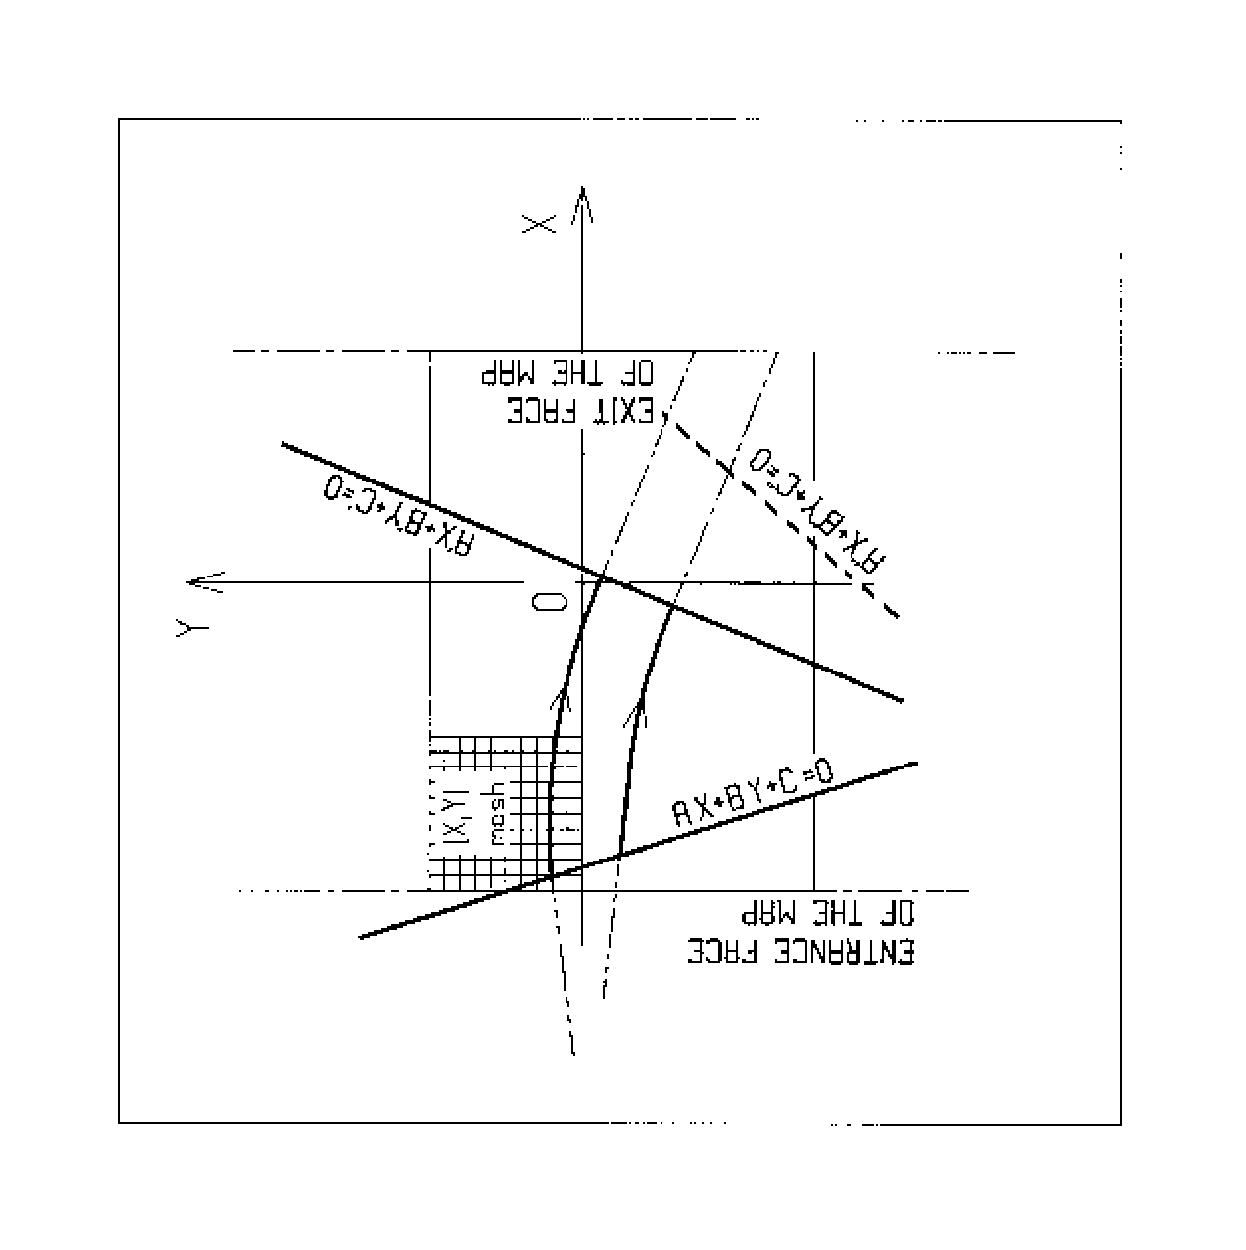
\includegraphics[height=15cm,angle=-90]{Fig15.ps}}
\caption[Fig15]{\label{fig15}$OXY $ is the coordinate system of the mesh.
Integration boundaries may be defined, using $ ID\not= 0 $~: particle coordinates are
extrapolated linearly from the entrance face of the map, onto the boundary 
$A'X+B'Y+C'=0$~; after ray-tracing inside the 
map and terminating on the boundary $AX+BY+C=0$, coordinates are
extrapolated linearly onto the exit face of the map if $ID=2$, or 
 terminated on the last ($ID-1$) boundary if $ID >2$.}
\end{figure}
\vfill
\newpage

\subsubsection*{CAVITE~: \CAVITETitl}  \label{CAVITE}\index{CAVITE|textbf}
\index{acceleration}\index{synchrotron motion}
\medskip

\textsl{CAVITE}  provides an  simulation of a (zero length)
accelerating cavity~; it can be used in conjunction with  keywords \REBELOTE\index{REBELOTE} 
and \textsl{SCALING} for 
the simulation of multiturn\index{multiturn} tracking with synchrotron acceleration (see section~\ref{sec4.6.4}). 
It must be preceded by \textsl{PARTICUL} for the definition 
of mass $ M $ and charge $ q$.   
\bigskip

\noindent\textbf{If $\mathbf{IOPT  =  0}$~:}   \textsl{CAVITE} is switched off.  
\bigskip

\noindent\textbf{If $\mathbf{IOPT  =  1}$~:}  \textsl{CAVITE} simulates the R.F.~cavity of a 
synchrotron 
accelerator. Normally the keyword \textsl{CAVITE} appears \textbf{at the end} of the optical 
structure (the periodic motion over $IT  = 1$, \textsl{NPASS} + 1 \index{NPASS}
turns is simulated by means of the keyword \textsl{REBELOTE\index{REBELOTE}}, option 
\mbox{K  =  99} while  R.F.  and optical elements  timings are simulated by means of
\textsl{SCALING} --- see section~\ref{sec4.6.4}). The synchrotron motion of any of the 
\IMAX\index{IMAX@{\IMAX}} particles of a beam is obtained by solving the following mapping 

$$ \left\{ 
\begin{array}{l}
	\phi_ 2-\phi_ 1= 2\pi \, f_{RF}\, 
	     \left(  \dfrac{\ell}{ \beta c} - \dfrac{\mathcal{L} }{ \beta_sc} \right) \\
	W_2-W_1 = q\hat  V\, \sin\phi_ 1  
\end{array}
\right. $$
%
 where
  
{\renewcommand{\arraystretch}{1}
 \begin{tabular}{>{$}l<{$}!{=}l}
	\phi        &  R.F. phase~; $\phi_ 2-\phi_ 1=$ variation  of $\phi$ between two  traversals\\
	W           &   kinetic  energy~;  $W_2-W_1=$ energy  gain  at  a traversal  of \textsl{CAVITE}\\
	\mathcal{L} & length  of  the  synchronous  closed orbit  (to  be  calculated  by  prior 
	              ray-tracing,\\
	 \multicolumn{1}{c}{  }           & see  the  bottom  NOTE) \\
	\ell        &  orbit length  of  the  particle  between  two  traversals\\
	\beta_ sc   &  velocity  of  the (virtual)  synchronous  particle\\
	\beta c     &  velocity  of  the  particle \\
	\hat  V     &  peak R.F.\ voltage\\
	q           &  particle  electric  charge.   
 \end{tabular}}
\bigskip

\noindent The R.F.\ frequency $ f_{RF} $ is a multiple of the synchronous 
revolution frequency, and is obtained from the input data, following 

$$ f_{RF} = \frac{hc }{\mathcal{L}}\, \frac{q(\Br )_s }{ \sqrt{q^2(\Br)^2_s+(Mc)^2}} $$
%
 where
  
 \begin{tabular}{l!{=}l}
   $h$ & harmonic  number  of  the  R.F\\
   $M$ &  mass  of  the  particle \\
   $c$ & velocity  of light.
  \end{tabular}
\bigskip

\noindent The current rigidity $ (\Br )_s $ of the synchronous particle is
obtained from the timing law specified by means of \textsl{SCALING} following 
$ (\Br)_s= \BORO\cdot \text{\textsl{SCALE(TIMING)}} $\index{BORO@{\BORO}} 
(see  \textsl{SCALING}  for the meaning and calculation of the scale 
factor \textsl{SCALE(TIMING)}). If \textsl{SCALING\index{SCALING}} is 
not used, $ (\Br )_s $ is assumed to keep the constant value \BORO
given in the object description (see \textsl{OBJET\index{OBJET}} for instance). \

\noindent The velocity $ \beta c $ of a particle is calculated from its
current rigidity

$$ \beta  = \frac{q(\Br ) }{ \sqrt{ q^2(\Br )^2+(Mc)^2}} $$
%
 The velocity $ \beta_ sc $ of the synchronous particle is obtained
in the same way from

$$ \beta_ s = \frac{q(\Br )_s }{ \sqrt{ q^2(\Br )^2_s + (Mc)^2}} $$
%
 The kinetic energies and rigidities involved in these formulae are related by

$$ q(\Br ) = \sqrt{ W(W+2Mc^2)} $$
%
 Finally, the initial conditions for the mapping, at the first 
turn, are the following  
\begin{itemize}
\item[-] For the (virtual) synchronous particle
%
\begin{align*}
	\phi_ 1 &  = \phi_ s = \text{synchronous phase}  \\
	(\Br )_{1s} & = \BORO  
\end{align*}

\item[-] For any of the $ I=1$,  \IMAX\index{IMAX@{\IMAX}}  particles of the beam 
%
\begin{align*}
	\phi_{1I} & = \phi_ s = \text{synchronous  phase} \\
	(\Br )_{1I} & =\BORO \ast  D_I
\end{align*}
%
where the quantities \BORO and $ D_I $ are given in the object description. 
\end{itemize}

\paragraph{Calculation of the coordinates} 

\noindent Let   $ p_I= \left[p^2_{XI}+p^2_{YI}+p^2_{ZI} \right]^{1/2} $ be the momentum of particle 
$ I $ at the exit of the cavity, while \\ %%%%% adjustment cesure peu satisfaisant !!
$ p_{I_0}= \left[p^2_{XI_0}+p^2_{YI_0} + p^2_{ZI_0}\right]^{1/2} $ is its 
momentum at the entrance. The kick in momentum is assumed to be 
fully longitudinal, resulting in the following relations between 
the coordinates at the entrance (denoted by the index zero) and at the exit 

 \begin{align*}
	 p_{XI} 
	      & = \left[p^2_I-(p^2_{I_0}-p^2_{XI_0}) \right]^{1/2} \\
	p_{YI} & = p_{YI_0},\quad \text{and} \quad  p_{ZI}= p_{ZI_0} \quad\text{(longitudinal  kick)} \\ 
	X_I &  = X_{I_0},\quad Y_I=Y_{I_0}\quad  \text{and} 
	        \quad Z_I=Z_{I_0} \quad\text{(zero  length cavity)}   
 \end{align*}
%
and for the angles (see Fig.~\ref{fig1})  
%
\begin{equation*}
	\left. 
	\begin{aligned}
		T_I & =  \text{Atg} \left( \dfrac{p_{YI}}{ p_{XI}} \right) \\
		P_I &  =  \text{Atg} \left(\dfrac{P_{ZI}}{(p^2_{XI}+p^2_{YI})^{1/2}} \right) 
	\end{aligned}
	 \right\rbrace \quad \text{(damping  of the  transverse  motion)}
\end{equation*}  
%\vfill\eject

\noindent\textbf{If $\mathbf{IOPT  =  2~:}$} the same simulation of a synchrotron R.F.\ cavity, 
as for $\mathbf{IOPT  =  1}$, is performed, except that the keyword 
\textsl{SCALING\index{SCALING}} (family \textsl{CAVITE\index{CAVITE}}) is not taken into 
account in this option~: the increase in kinetic energy at each traversal, 
for the synchronous particle, is

$$ \Delta W_s= q\hat  V \,\sin\phi_ s $$
%
where the synchronous phase $ \phi_ s $ is given in the input data.
From this, the calculation of the law $ (\Br )_s $ and the R.F.\ frequency 
$f_{RF} $ follows, according to the formulae given in \mbox{\textsl{IOPT}  =  1}. 
\bigskip

\noindent\textbf{If $\mathbf{IOPT  =  3}$~:} acceleration without synchrotron motion. 
Any particle will be given a kick

$$ \Delta W = q\hat  V\, \sin\phi_ s $$
%
where $ \hat  V $ and $ \phi_ s $ are input data.  
\bigskip

\noindent NOTE~: Calculation of the closed orbit. \\
Due to the fringe fields, the horizontal closed orbit may not 
coincide with the ideal axis of the optical elements. One way to 
calculate it at the beginning of the structure (\emph{i.e.}\ where the 
initial particle coordinates have to be defined) is to ray-trace 
a single particle over a sufficiently large number of turns, 
starting with the initial condition $ (Y_0=T_0=Z_0=P_0=0)$,  and so as to 
obtain a statistically well-defined phase-space ellipse. The 
initial conditions of the closed orbit then correspond to the 
coordinates $ Y_c $ and $ T_c $ of the center of this ellipse. Next, 
ray-tracing over one turn a particle starting with the initial condition 
($Y_c $, $ T_c $, $ Z_0=P_0=0$)  will provide the length $\mathcal{L}$ 
(namely, the $ F(6,1) $ coordinate) of the closed orbit. 

\newpage

\subsubsection*{CHAMBR~:  \CHAMBRTitl}\label{CHAMBR}\index{CHAMBR|textbf} 
\medskip

\textsl{CHAMBR} causes the identification, counting and stopping of 
particles that reach the 
transverse limits of the vacuum chamber.  The chamber can be either rectangular 
(\textsl{IFORM} = 1) or elliptic (\textsl{IFORM} = 2). The chamber is centered
at $ YC$, $ZC $ and has transverse dimensions $\pm YL $ and  
$\pm  ZL $ such that any particle will be stopped\index{stopped particles} if its coordinates $ Y,Z $ satisfy 

\begin{align*}
	(Y-YC)^2\geq  YL^2  \text{ or }   (Z-ZC)^2 \geq  ZL^2 
	   &   \quad \text{if}\quad  \text{\textsl{IFORM}}=1  \\
	\dfrac{ (Y-YC)^2 }{ YL^2} + \dfrac{(Z-ZC)^2 }{ ZL^2} \geq 1  
	  &   \quad \text{if}\quad  \text{\textsl{IFORM}}=2  
\end{align*}

\noindent The conditions introduced with \textsl{CHAMBR\index{CHAMBR}} are valid
along  the optical structure until the next occurrence  of the keyword \textsl{CHAMBR}.  Then, if
$ \IL=1 $ the aperture is possibly modified by introducing new values of $ YC$,  $ ZC$, 
 $YL $ and $ ZL $, or, if $ \IL=2 $ the chamber ends and information is 
printed concerning those particles that have been stopped.  
\bigskip

\noindent The testing is done in optical elements at each integration step, between the
\textsl{EFB}'s. For instance, in \textsl{QUADRUPO\index{QUADRUPO}} there will be 
no testing from $-X_E $ to 0 and 
from $ \XL $ to $ \XL+X_S $, but only from 0  to $ \XL $~;  in \textsl{DIPOLE\index{DIPOLE}}, there is no 
testing as long as the \textsl{ENTRANCE EFB} is not reached, and testing is stopped as 
soon as the \textsl{EXIT} or \textsl{LATERAL EFB}'s are passed.  
\bigskip

\noindent In polar coordinate optical elements $ Y $  stands for the radial
coordinate (e.g. with \textsl{DIPOLE\index{DIPOLE}}, see Figs.~\ref{fig3}C and~\ref{fig9}).  
 Therefore, centering \textsl{CHAMBR\index{CHAMBR}} at $ YC=RM $ simulates a chamber curved with radius 
 $ RM $, and having a radial acceptance $ RM\pm YL $.  The testing  is done in  \textsl{ESL}  
 (\textsl{DRIFT}) at the beginning and the end, and only for positive drifts.  There 
is no testing in \textsl{CHANGREF\index{CHANGREF}}.  
\bigskip

\noindent When a particle is stopped\index{stopped particles}, its index 
\IEX\index{IEX@{\IEX}}  (see \textsl{OBJET\index{OBJET}} and 
section~\ref{sec4.6.6}) is set to the value -4, and its actual path length is stored in the array 
\textsl{SORT} for possible further statistical purposes. 




\newpage

\subsubsection*{CHANGREF~: \CHANGREFTitl} \label{CHANGREF}\index{CHANGREF|textbf}
\medskip

\CHANGREF {it transports} the particles to a new reference frame.  It can be used anywhere 
in a structure.  The new coordinates of the particles  $ Y_2$,  $ T_2$,  $ Z_2$ and 
$ P_2 $ and the path length $ S_2 $ are deduced from the old ones  $ Y_1$,   
$ T_1$,  $ Z_1$,  $ P_1 $ and $ S_1 $ by
%
\begin{figure}[h]
\begin{minipage}{.4\linewidth}
\begin{align*}
	T_2 &=  T_1- \text{\textsl{ALE}} \\
	Y_2 & = \dfrac{ (Y_1-YCE) \cos T_1+XCE \sin T_1}{\cos  T_2} \\
	DL^2 & =(XCE-Y_2 \sin \text{\textsl{ALE}})^2 
	         +(YCE-Y_1+Y_2 \cos \text{\textsl{ALE}})^2 \\
	Z_2  & = Z_1+DL\mathrm{tg} P_1 \\ 
	S_2 & = S_1+ \dfrac{DL }{ \cos P_1} \\
	P_2 & = P_1  
\end{align*}
\end{minipage}
\begin{minipage}{.5\linewidth}
\centerline{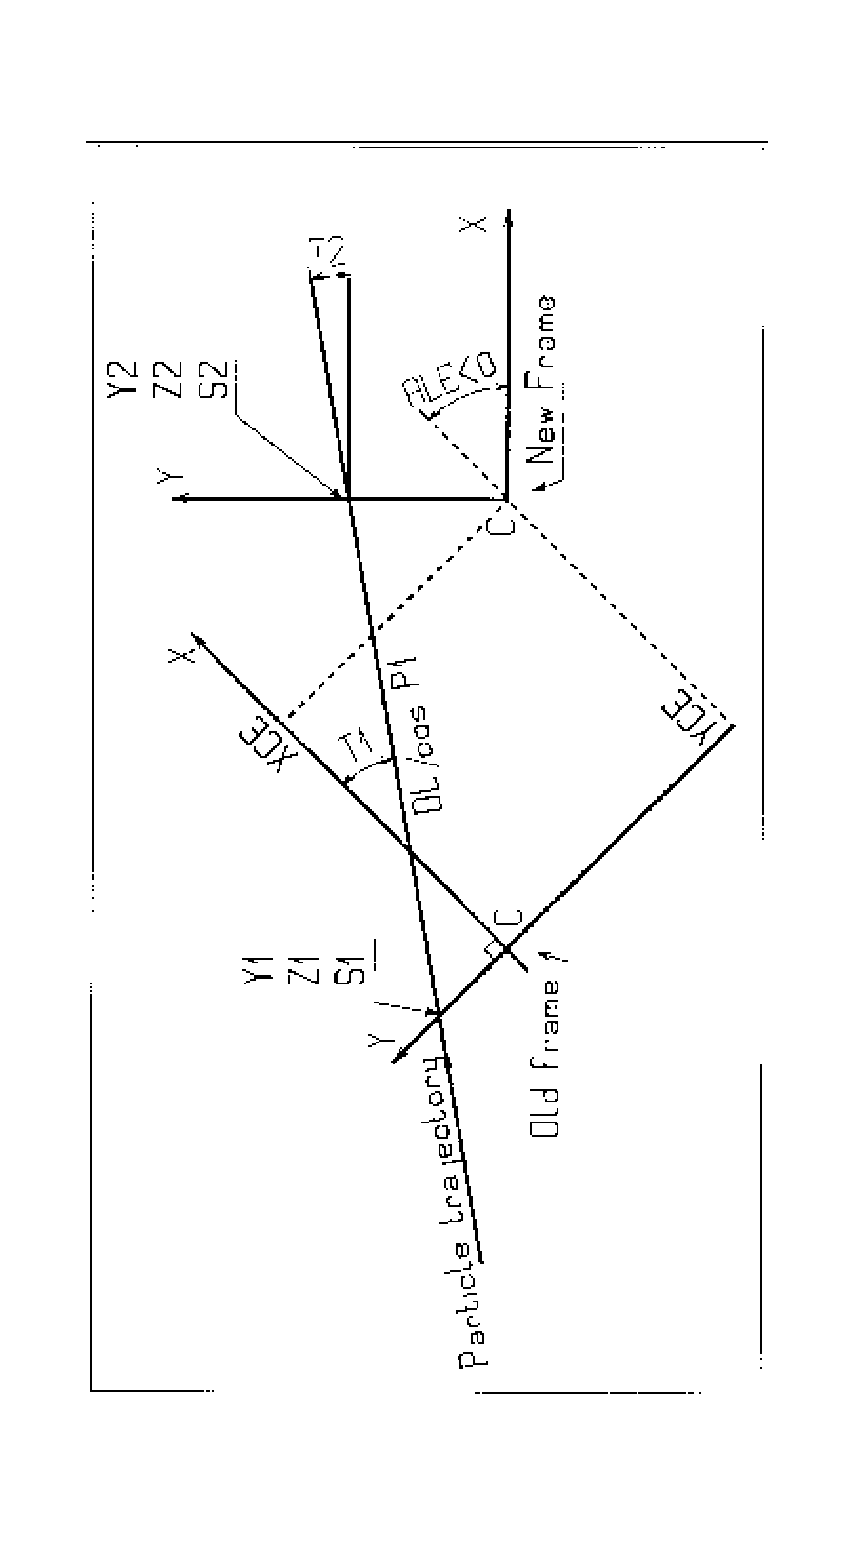
\includegraphics[height=8.5cm,angle=-90]{FigCHAREFa.eps}}
\hangcaption{\label{FigCHAREFa}Scheme of the \CHANGREF procedure. }
\end{minipage}
\end{figure}
%
\noindent where, $ XCE $ and $ YCE $ are shifts in the horizontal plane along,respectively, 
$ X$- and $ Y$-axis, and \textsl{ALE}  is a rotation around the $ Z$-axis. $ DL $
is given the sign of $ XCE-Y_2 \sin(\text{\textsl{ALE}})$.  

\noindent This keyword may for instance be used
for positioning optical elements, or for setting a reference frame at the entrance
or exit of field maps, or to simulate misalignements (see also  \textsl{KPOS}).  \\
Effects of \CHANGREF on spin tracking\index{spin tracking}, 
particle decay and gas-scattering are taken into account (but not on synchrotron radiation).
\vfill
%%%%%%%%%%%%%%figure%%%%%%%%%%%%%%
%\begin{figure}[H]
%%\vspace{10.5 truecm}
%%%%Figure 16
%\centerline{\includegraphics[height=15cm,angle=-90]{Fig16.ps}}
%\hangcaption{\label{fig16}Scheme of the \CHANGREF procedure. }
%\end{figure}

\bigskip

\noindent The example below shows the use of  \CHANGREF\ for the symmetric positioning of 
a dipole+quadrupole  magnet in a drift-bend-drift geometry with 
12.691~degrees deviation (obtained upon combined effect of  a dipole component and 
of quadrupole axis shifted 1~cm off optical axis). 

\medskip

\begin{center}
\begin{minipage}{.38\linewidth}

 Zgoubi data file~: 

\tiny
\begin{verbatim}
Using CHANGREF
'OBJET'
51.71103865921708                          Electron, Ekin=15MeV.
2
1 1                                           One particle, with
2. 0.  0.0 0.0 0.0 1. 'R'      Y_0=2 cm, other coordinates zero.
1 1 1 1 1 1 1 
'MARKER'    BEG    .plt                -> list  into zgoubi.plt.
'DRIFT'                                             10 cm drift.
10.
'CHANGREF'  
0. 0. -6.34165                              First half z-rotate.
'CHANGREF'  
0. 1. 0.                                           Next Y-shift.
'MULTIPOL'     Combined function multipole, dipole + quadrupole.
   2                                   -> list  into zgoubi.plt.
5  10. 2.064995867082342  2. 0. 0. 0. 0. 0. 0. 0. 0.
 0 0  5. 1.1  1.00 1.00 1.00 1.00 1.00 1. 1. 1. 1.                              
4  .1455   2.2670  -.6395  1.1558  0. 0.  0.                                    
 0 0  5. 1.1  1.00 1.00 1.00 1.00 1.00 1. 1. 1. 1.                              
4  .1455   2.2670  -.6395  1.1558  0. 0.  0.                                    
0 0 0 0 0 0 0 0 0 0
.1   step size
1  0. 0.  0.
'CHANGREF'
0. -1. -6.34165          First Y-shift back, next half z-rotate.
'DRIFT'                                             10 cm drift.
10.
'MARKER'    END    .plt                -> list  into zgoubi.plt.
'FAISCEAU'
'END'
\end{verbatim}
\normalsize
\end{minipage}\hspace{.05\linewidth}
\begin{minipage}{.5\linewidth}
\centerline{\includegraphics*[bbllx=20,bblly=100,bburx=567,bbury=470,width=8cm]{FigCHAREFb.eps}}

Note~: The square markers scheme the stepwise integration in case of $\pm$5~cm additional fringe field 
extent upstream and downstream of the 5~cm long multipole. 
\end{minipage}
\end{center}


\vfill




\newpage

\subsubsection*{CIBLE or TARGET~: \CIBLETitl}
\label{CIBLE}\label{TARGET}
\index{CIBLE|textbf} \index{TARGET|textbf}
\medskip

 The reaction is $ 1+2 \longrightarrow  3+4 $ with the following parameters 
$$
\begin{array}{lllll}
	\text{Laboratory momentum} & p_1\equiv  0 &  p_2 &   p_3 &    p_4 \\
	\text{Rest mass}           &   M_1        &   M_2 & M_3 &    M_4 \\ 
	\text{Total energy in laboratory} & M_1c^2 &  W_2 &    W_3 &   W_4 
\end{array}
$$
%
 The geometry of the interaction is shown in Fig.~\ref{fig17}.   
\medskip

\noindent The angular  sampling at the exit of the target consists of the $ NT$ 
coordinates 0,  $ \pm TS$,  $ \pm 2\ast TS$...   $\pm (NT-1)\ast TS/2 $ 
in the median plane, 
and the $ NP $ coordinates 0, $ \pm PS$,  $ \pm 2\ast PS$... $ \pm (NP-1)\ast PS/2$ 
in the vertical plane.  
\medskip

\noindent The position of $ B $ downstream is deduced from that of $ A $
upstream  by a transformation equivalent to two transformations using \textsl{CHANGREF\index{CHANGREF}},
 namely
 \begin{gather*}
	 \text{\textsl{CHANGREF}}(XCE=YCE=0,\quad  \textsl{ALE}=\beta )  \\
\intertext{followed by} 
	 \text{\textsl{CHANGREF}}(XCE=YCE=0,\quad \textsl{ALE}=\theta -\beta ). 
 \end{gather*}

 
\noindent Particle  4 is discarded, while particle 3 continues. The energy
loss $ Q $ is related to the variable mass $ M_4 $ by
$$ Q=M_1+M_2-(M_3+M_4)\qquad \text{and} \qquad dQ=-dM_4 $$

\noindent The momentum sampling of particle 3 is derived from conservation of
energy and 
momentum, according to 

\begin{align*}
	M_1c^2+W_2 & =  W_3+W_4  \\
	p^2_4 & =  p^2_2 +p^2_3 -2p_2p_3 \cos (\theta -T) 
\end{align*}


%%%%%%%%%%%%%%figure%%%%%%%%%%%%%%
\begin{figure}[H]
%\vspace{17 truecm}
%%%Figure 17
\centerline{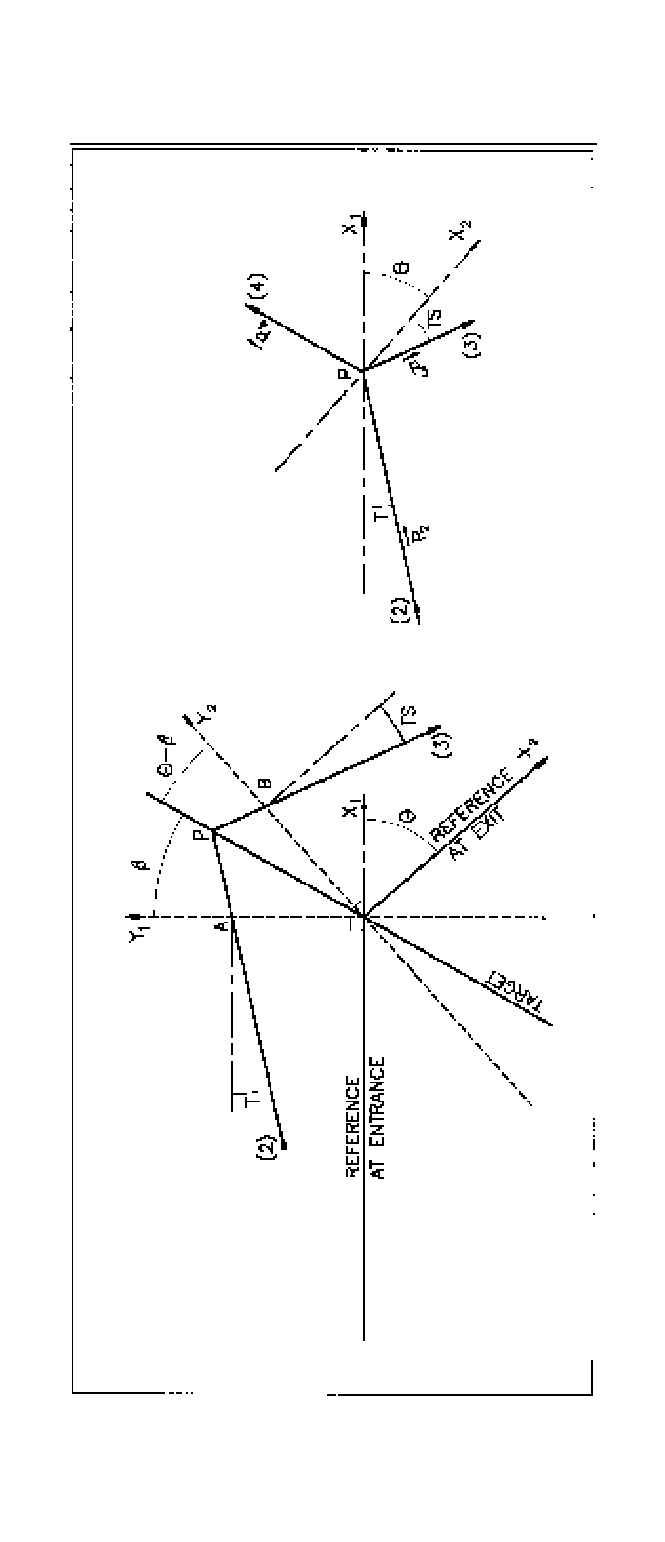
\includegraphics[height=15cm,angle=-90]{Fig17.ps}}
{\setlength{\captionwidth}{14cm}
\hangcaption[Fig17]{\label{fig17}Scheme of the principles of \textsl{CIBLE (TARGET)}\\
 $ A, T$   =   position, angle of incoming particle 2 in the entrance reference frame\\
 $P$   =   position of the interaction\\
 $B, T$   =   position, angle of the secondary particle  in the exit reference frame\\ 
 $\theta$   =   angle between entrance and exit frames\\
 $\beta$   =   tilt angle of the target}     }
\end{figure}
\vfill

\newpage

\subsubsection*{COLLIMA~: \COLLIMATitl}\label{COLLIMA}\index{COLLIMA|textbf}
\medskip

\textsl{COLLIMA}  acts as a mathematical aperture of zero length.  It causes 
the identification, counting and stopping of particles that reach the aperture limits.  

\paragraph{Physical aperture}

\noindent A physical aperture can be either rectangular (\textsl{IFORM} = 1) or elliptic 
(\textsl{IFORM} = 2).  The collimator is centered at $ YC$, $ZC $ and has transverse
dimensions $\pm YL $ and $\pm ZL $ such that any particle will be
stopped\index{stopped particles} if its coordinates $Y$, $Z $ satisfy
\begin{align*}
	(Y-YC)^2\geq  YL^2  \text{ or }   (Z-ZC)^2 \geq  ZL^2 
	   &   \quad \text{if}\quad  \text{\textsl{IFORM}}=1  \\
	\dfrac{ (Y-YC)^2 }{ YL^2} + \dfrac{(Z-ZC)^2 }{ ZL^2} \geq 1  
	  &   \quad \text{if}\quad  \text{\textsl{IFORM}}=2  
\end{align*}

\paragraph{Longitudinal collimation} 

\noindent \textsl{COLLIMA}  can act as a longitudinal phase-space aperture, coordinates acted on are 
selected with  \textsl{IFORM.J}. 
Any particle will be stopped  if its horizontal  (h) and vertical (v) coordinates satisfy 
\begin{align*}
	 (h \leq h_{min} \textrm{~or~} h \geq  h_{max})  ~\textrm{~or~}~  (v \leq v_{min}  \textrm{~or~}  v \geq  v_{max})
\end{align*}
wherein, $h$ is either path length $S$ if \textsl{IFORM}=6 or time  if \textsl{IFORM}=7, and 
$v$  is either 1+DP/P if \textsl{J}=1 or kinetic energy  if \textsl{J}=2 (provided mass and charge have 
been defined using the keyword \textsl{PARTICUL\index{PARTICUL}}). 

\noindent If \textsl{IFORM}=11 (respectively 12) then $\epsilon_Y/\pi$  (respectively $\epsilon_Z/\pi$) 
is to be specified by the user as well as $\alpha_{Y,Z}$, $\beta_{Y,Z}$. 
If \textsl{IFORM}=14 (respectively 15) then $\alpha_Y$ and  $\beta_Y$  (respectively $\alpha_Z$,  $\beta_Z$) 
are computed by \zgoubi\ by prior 
matching of the particle population, only $\epsilon_{Y,Z}/\pi$ need be specified by the user. 



\paragraph{Phase-space collimation}

\noindent \textsl{COLLIMA}  can act as a phase-space aperture. 
Any particle will be stopped\index{stopped particles} if its coordinates satisfy 
\begin{align*}
	\gamma_Y Y^2 + 2\alpha_Y Y T + \beta_Y T^2 \geq  \epsilon_Y/\pi 
	   &   \quad \text{if}\quad  \text{\textsl{IFORM}}=11  \text{ or 14} \\
	\gamma_Z Z^2 + 2\alpha_Z Z P + \beta_Z P^2 \geq  \epsilon_Z/\pi 
	   &   \quad \text{if}\quad  \text{\textsl{IFORM}}=12  \text{ or 15}
\end{align*}

\noindent If \textsl{IFORM}=11 (respectively 12) then $\epsilon_Y/\pi$  (respectively $\epsilon_Z/\pi$) 
is to be specified by the user as well as $\alpha_{Y,Z}$, $\beta_{Y,Z}$. 
If \textsl{IFORM}=14 (respectively 15) then $\alpha_Y$ and  $\beta_Y$  (respectively $\alpha_Z$,  $\beta_Z$) 
are computed by \zgoubi\ by prior 
matching of the particle population, only $\epsilon_{Y,Z}/\pi$ need be specified by the user. 




\bigskip

\noindent When a particle is stopped, its index \IEX\index{IEX@{\IEX}} (see \textsl{OBJET}
and section~\ref{sec4.6.6}) is set to the value -4, and its actual path length is stored in 
the array \textsl{SORT}  for possible further statistical purposes (e.g.~with 
\textsl{HISTO\index{HISTO}}). 


\newpage

\subsubsection*{DECAPOLE~:  \DECAPOLETitl\ (Fig.~\protect\ref{fig18})} \label{DECAPOLE} \index{DECAPOLE|textbf}
\medskip

The meaning of parameters for \textsl{DECAPOLE}  is the same as for \textsl{QUADRUPO\index{QUADRUPO}}.  
%\bigskip

\noindent In fringe field regions the magnetic field $ \vec  B(X,Y,Z) $ and
its derivatives up to fourth order are derived from the scalar potential approximated to 
the 5th order in $ Y $ and $ Z $ 

\begin{align*}
	V(X,Y,Z) &   =    G \left(Y^4Z-2Y^2Z^3+ \dfrac{Z^5 }{ 5}\right)  \\
	\text{with  } G_0 &   = \dfrac{ B_0 }{ R^4_0} 
\end{align*}


\noindent Outside fringe field regions, or everywhere in sharp edge decapole 
($ \lambda_ E=\lambda_ S=0$) , $ \vec  B(X,Y,Z) $ in the magnet is given by 

\begin{align*}
	B_X &   =    0 \\
	B_Y &   =   4G_0(Y^2-Z^2)YZ \\
	B_Z &   =    G_0(Y^4-6Y^2Z^2+Z^4)
\end{align*}
\vfill

%%%%%%%%%%%%%%figure%%%%%%%%%%%%%%
\begin{figure}[H]
%\vspace{12 truecm}
%%%Figure 18
\centerline{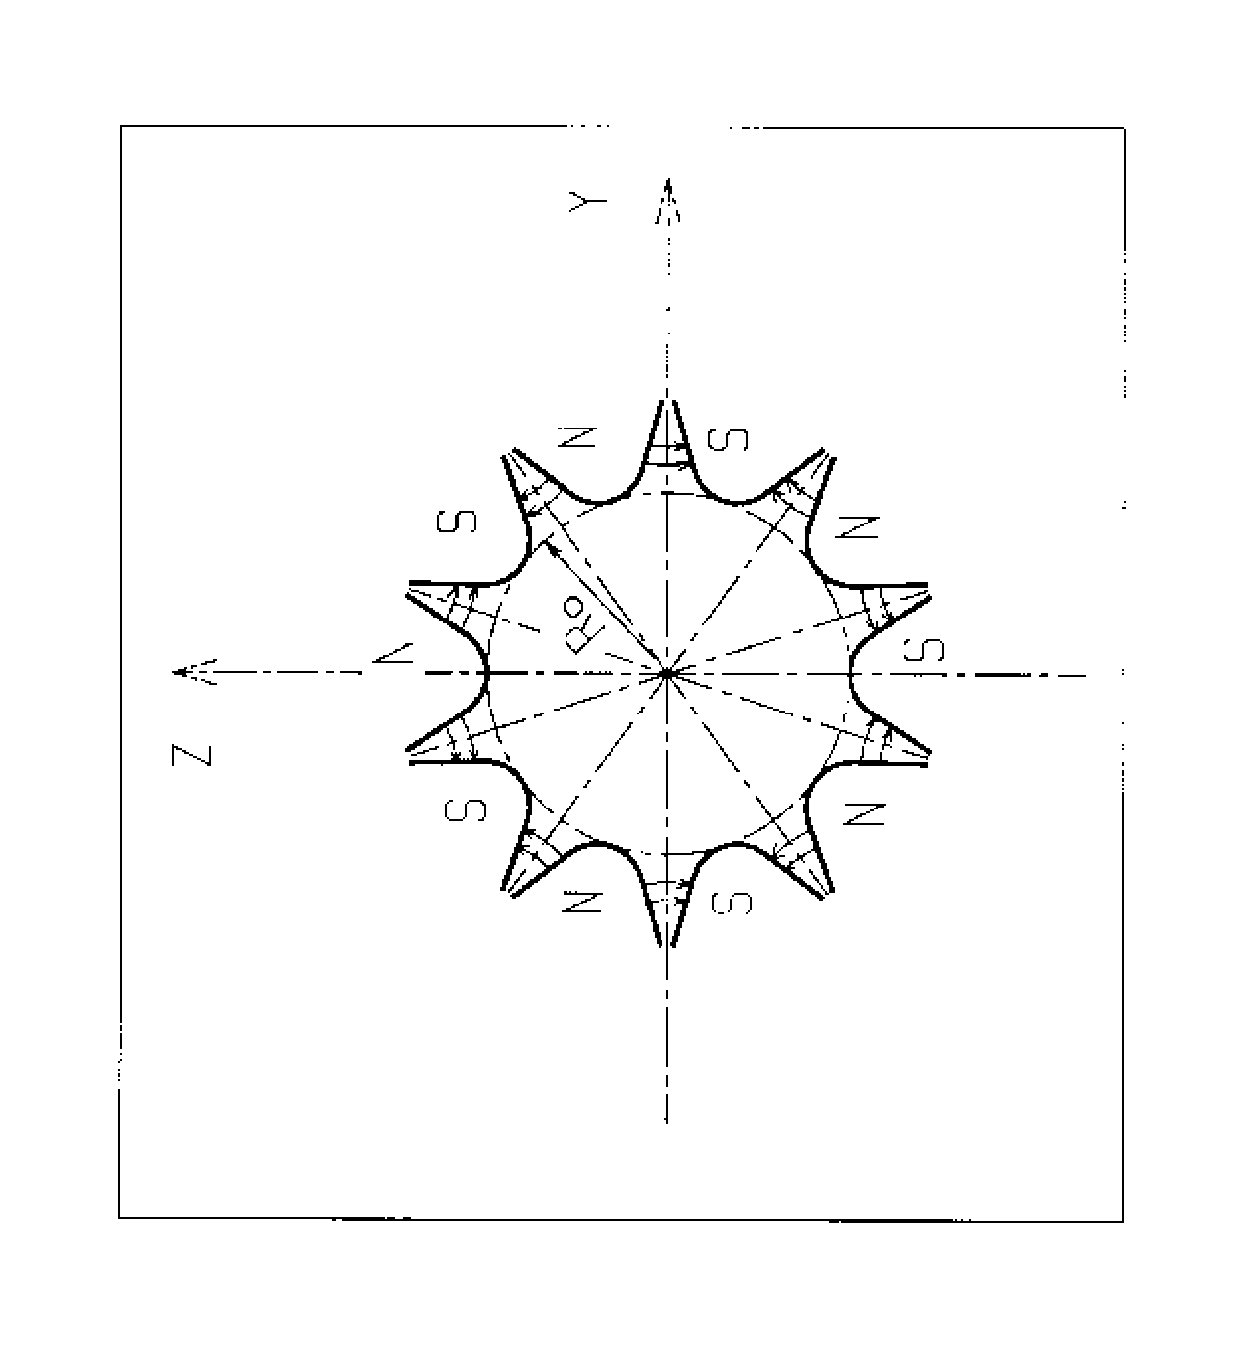
\includegraphics[width=12cm,angle=-90]{Fig18.ps}}
\caption{\label{fig18}Decapole magnet}
\end{figure}
\vfill








\newpage

\subsubsection*{DIPOLE~: \DIPOLETitl} \label{DIPOLE} \index{DIPOLE|textbf}
\medskip

\noindent\textsl{DIPOLE} provides a model of a dipole field, possibly with transverse indices. 
 The field along a particle trajectory is computed as the 
particle motion proceeds, straightforwardly from the dipole geometrical parametres. 
To make it more precise, field simulation model in \textsl{DIPOLE}  is the same as used in \textsl{DIPOLE-M} and \textsl{AIMANT} 
for computing a field map~; the main difference in \textsl{DIPOLE} is in its skipping that 
intermediate step of field map generation found in \textsl{DIPOLE-M} and \textsl{AIMANT}. 

\bigskip

\noindent These are handled as follows. The dimensionning of the magnet is defined by

\bigskip

 \begin{tabular}{>{\sl}l!{~:}l}
	 AT &  total angular aperture \\
	 RM & mean radius used for the positioning of field boundaries\\
 \end{tabular}

\bigskip

The 2 or 3 effective field boundaries (EFB), from which  the dipole field  is drawn, are
defined from geometric boundaries, the shape and position of which are determined by the 
following parameters. 

\bigskip

\begin{tabular}{l!{~:}l}
	 \textsl{ACENT} 
	    & arbitrary inner angle, used for EFB's positioning  \\
	$\omega$ &  azimuth of an EFB with respect to  \textsl{ACENT}\\
	$\theta$ & angle of an EFB with respect to its azimuth (wedge angle)\\ 
	$R_1$, $R_2$  &  radius of curvature of an EFB\\
	$U_1$, $U_2$  &  extent of the linear part of an EFB. 
\end{tabular}

\bigskip


 \noindent The magnetic field is calculated in  polar
coordinates. At  any position $(R,\theta)$ along the  particle trajectory 
the value of the vertical component of the mid-plane field is calculated by 
 \begin{equation}
	 B =  \mathcal{F(R,\theta)} \ast  B_0 \ast  
	      \left(1+N \ast  
	           \left( \frac{R-RM }{ RM}\right) 
	           + B \ast  \left(\frac{R-RM }{ RM} \right)^2 
	           + G \ast  \left(\frac{R-RM }{ RM} \right)^3 
	      \right) 
 	%\label{eq3-3-1}
 \end{equation}
 where  $ N$, $B $ and $ G $ are  respectively  the first, second and
third order field indices and $ \mathcal{F}(R,\theta)$ is the fringe field coefficient. 


\paragraph{Calculation of the Fringe Field Coefficient} 

\noindent With  each EFB a realistic extent of the fringe field, $\lambda$ 
(normally equal to the gap size), is associated and a fringe field coefficient
$ F $ is calculated. In the following $\lambda$ stands for either $ \lambda_ E $
(Entrance), $ \lambda_ S $ (Exit) or $ \lambda_ L $ (Lateral EFB).  


\bigskip

\noindent$ F $ is an exponential type fringe field (Fig.~\ref{fig11}) 
given by~\cite{Biblio12}     %%% [12]

$$ F = \frac{1 }{ 1+ \exp P(s)} $$
%
 wherein $ s $ is the distance to the EFB and depends on $(R,\theta)$, and 

$$
    P(s) = C_0
       +C_1 \left(  \dfrac{s }{ \lambda} \right) 
       +C_2 \left( \dfrac{s }{ \lambda} \right)^2 
       + C_3 \left( \dfrac{s }{ \lambda} \right)^3 
       +C_4 \left( \dfrac{s }{ \lambda} \right)^4 
       + C_5 \left(\dfrac{s }{ \lambda} \right)^5 $$
       
\noindent It is also possible to simulate a shift of the \textsl{EFB}, by giving a non
zero value to the parameter \textsl{SHIFT}.  $ s $ is then changed to $ s -$\textsl{SHIFT} in the 
previous equation.   This allows small variations of the magnetic length.  
\bigskip

\noindent Let $ F_E $ (respectively $ F_S$, $F_L$)  be the fringe field
coefficient attached to the entrance (respectively exit, lateral) EFB. At any position on  a 
trajectory the resulting value of the fringe field coefficient (eq.~\ref{eq3-3-1}) is

$$  \mathcal{F}(R,\theta) = F_E  \ast  F_S \ast   F_L $$
%
($F_L=1 $ if no lateral EFB is requested). 



\paragraph{Simulating Field Defects and Shims }

\noindent Not provisionned in the present version. 

\bigskip


\paragraph{Calculation of the  mid-plane field derivatives }

This is performed using the numerical interpolation method based on a flying grid as described in 
the \textsl{DIPOLES} procedure (page~\pageref{CalcMidPlaneFieldInterpol}). 

\bigskip

\paragraph{Extrapolation Off Median Plane} 

\noindent From the vector field $ \vec  B $ and  derivatives in the median plane, 
first a transformation from polar to Cartesian coordinates is 
performed, following eqs (\ref{eq2-4-8} or \ref{eq2-4-9}), then,  extrapolation off median plane is 
performed by means of Taylor expansions, following the procedure described in section~\ref{sec2.3.2}. 






\newpage

\subsubsection*{DIPOLE-M~: \DIPOLEMTitl} \label{DIPOLE-M} \index{DIPOLE-M|textbf}
\medskip

\noindent\textsl{DIPOLE-M} is a more recent, simpler and improved version of 
\textsl{AIMANT\index{AIMANT}}.  
\bigskip

\noindent The keyword \textsl{DIPOLE-M} provides an automatic generation of a dipole 
field map in polar coordinates. The extent of the map is defined by the 
following parameters, as shown in Figs.~\ref{fig9}A and~\ref{fig9}B.
\bigskip

 \begin{tabular}{>{\sl}l!{~:}l}
	 AT &  total angular aperture\\
	 RM & mean radius used for the positioning of field boundaries\\
	 RMIN, RMAX
	    &  minimum and maximum radii 
 \end{tabular}
\bigskip
 
\noindent The 2 or 3 effective field boundaries (EFB) inside the map are
defined from geometric boundaries, the shape and position of which are determined by the 
following parameters. 
\bigskip

\begin{tabular}{l!{~:}l}
	 \textsl{ACENT} 
	    & arbitrary inner angle, used for EFB's positioning  \\
	$\omega$ &  azimuth of an EFB with respect to  \textsl{ACENT}\\
	$\theta$ & angle of an EFB with respect to its azimuth (wedge angle)\\ 
	$R_1$, $R_2$  &  radius of curvature of an EFB\\
	$U_1$, $U_2$  &  extent of the linear part of an EFB. 
\end{tabular}
\bigskip


\noindent At  any node  of the map mesh, the value of the field is calculated as 
 \begin{equation}
	 B =  \mathcal{F} \ast  B_0 \ast  
	      \left(1+N \ast  
	           \left( \frac{R-RM }{ RM}\right) 
	           + B \ast  \left(\frac{R-RM }{ RM} \right)^2 
	           + G \ast  \left(\frac{R-RM }{ RM} \right)^3 
	      \right) 
 	\label{eq3-3-1}
 \end{equation}
%
 where  $ N$, $B $ and $ G $ are  respectively  the first, second and
third order field indices and $ \mathcal{F}$ is the fringe field coefficient. 


\paragraph{Calculation of the Fringe Field Coefficient} 

\noindent With  each EFB a realistic extent of the fringe field, $\lambda $ 
(normally equal to the gap size), is associated and a fringe field coefficient
$ F $ is calculated. In the following $\lambda$ stands for either $ \lambda_ E $
(Entrance), $ \lambda_ S $ (Exit) or $ \lambda_ L $ (Lateral EFB).  
\bigskip

\noindent$ F $ is an exponential type fringe field (Fig.~\ref{fig11}) 
given by~\cite{Biblio12}     %%% [12]

$$ F = \frac{1 }{ 1+ \exp P(s)} $$
%
 where $ s $ is the distance to the EFB, and 

$$
    P(s) = C_0
       +C_1 \left(  \dfrac{s }{ \lambda} \right) 
       +C_2 \left( \dfrac{s }{ \lambda} \right)^2 
       + C_3 \left( \dfrac{s }{ \lambda} \right)^3 
       +C_4 \left( \dfrac{s }{ \lambda} \right)^4 
       + C_5 \left(\dfrac{s }{ \lambda} \right)^5 $$
       
\noindent It is also possible to simulate a shift of the \textsl{EFB}, by giving a non
zero value to the parameter \textsl{SHIFT}.  $ s $ is then changed to $ s -$\textsl{SHIFT} in the 
previous equation.   This allows small variations of the total magnetic length.  
\bigskip

\noindent Let $ F_E $ (respectively $ F_S$, $F_L$)  be the fringe field
coefficient attached to the entrance (respectively exit, lateral) EFB. At any node of the map 
mesh, the resulting value of the fringe field coefficient (eq.~\ref{eq3-3-1}) is

$$  \mathcal{F} = F_E  \ast  F_S \ast   F_L $$
%
($F_L=1 $ if no lateral EFB is requested). 

\paragraph{The Mesh of the Field Map} 

\noindent The magnetic field is calculated at the nodes of a mesh with polar
coordinates, in the median plane.  The radial step is given by 

 \begin{align*}
	 \delta R & = \dfrac{\text{\textsl{RMAX}} - \text{\textsl{RMIN}} }{\text{\textsl{IRMAX}}-1} \\
	\intertext{and the angular step by} 
	 \delta \theta  & = \dfrac{AT }{\text{\textsl{IAMAX}}-1} 
 \end{align*}
 %
\noindent where, \RMIN  and \RMAX   are the lower and upper
radial limits of the field map, and $ AT $ is its total angular aperture (Fig.~\ref{fig9}B).  
 \textsl{IRMAX}  and \textsl{IAMAX} are 
the total number of nodes in the radial and angular directions. 

\paragraph{Simulating Field Defects and Shims }

\noindent Once the initial map is calculated, it is possible to modify it by
means of the parameter \textsl{NBS}, so as to simulate field defects or shims. 
\bigskip

\noindent\textbf{If $\mathbf{NBS = - 2}$,} the map is globally modified by a
perturbation proportional to $ R-R_0 $, 
where $ R_0 $ is an arbitrary radius, with an amplitude $ \Delta B_Z/B_0 $, so
that $ B_Z $ at the nodes of the mesh is replaced by 

$$ B_Z  \ast   \left(1+ \frac{\Delta B_Z }{ B_0}\, \frac{R-R_0 }{\text{\RMAX- \RMIN}} \right) $$

\noindent\textbf{If  $\mathbf{NBS =  - 1}$,} the perturbation is proportional to
$ \theta -\theta_ 0 $, and $ B_Z $ is replaced by 

$$ B_Z \ast  \left(1+ \frac{\Delta B_Z }{ B_0} \, \frac{\theta -\theta_ 0 }{ AT}\right) $$

\noindent\textbf{If  $\mathbf{NBS \geq 1}$,} then \textsl{NBS} shims are introduced at
positions $ \dfrac{ R_1+R_2 }{ 2}$, $\dfrac{\theta_ 1+\theta_ 2 }{ 2} $ 
(Fig.~\ref{fig13})~\cite{Biblio13}   %%%   [13] 

\noindent The initial field map is modified by shims with second order profiles given by 

$$ \theta  = \left(\gamma  + \frac{\alpha }{ \mu} \right) \,\beta\, \frac{X^2 }{\rho^ 2} $$
%
 where $ X $ is shown in  Fig.~\ref{fig11}, 
 $\rho = \dfrac{R_1+R_2 }{ 2} $ is the central radius, $\alpha$ and $\gamma$ are the angular 
 limits of the shim, $\beta$ and $\mu$ are parameters. 
 
\noindent At each shim, the value of $ B_Z $ at any node of the initial map is replaced by 

$$ B_Z \ast  \left(1+F\theta  \ast  FR \ast  \frac{\Delta B_Z }{ B_0} \right)
$$
%
 where $ F\theta =0 $ or $ FR=0 $ outside the shim, and $ F\theta =1$ and $ FR=1 $ inside.  
\bigskip

\paragraph{Extrapolation Off Median Plane} 

\noindent The vector field $ \vec  B $ and its derivatives in the median plane
are calculated by means of a second or fourth order polynomial 
interpolation, depending 
on the value of the parameter \textsl{IORDRE\index{IORDRE}} (\textsl{IORDRE}=2, 25 or 4, see 
section~\ref{sec2.4.2}). 
The transformation from polar to Cartesian coordinates is 
performed following eqs (\ref{eq2-4-8} or \ref{eq2-4-9}). Extrapolation off median plane is then 
performed by means of Taylor expansions, following the procedure described 
in section~\ref{sec2.3.2}. 









\newpage

\subsubsection*{DIPOLES~: \DIPOLESTitl~\cite{reportNIMFFAG}} \label{DIPOLES} \index{DIPOLES|textbf}
\medskip

\noindent \textsl{DIPOLES} works much like \textsl{DIPOLE\index{DIPOLE}} 
as to the field modelling, yet with the particularity that it allows positioning up to 5 such 
dipoles within the angular sector with full aperture $AT$ thus allowing 
accounting for overlapping fringe fields\index{fringe fields!overlapping}  
This is done in the following 
way\footnote{\textsl{FFAG} can be referred to as another instance of a procedure based on such method.}. 

\bigskip

\noindent  The dimensionning of the magnet is defined by

\bigskip

 \begin{tabular}{>{\sl}l!{~:}l}
	 AT &  total angular aperture \\
	 RM & mean radius used for the positioning of field boundaries\\
 \end{tabular}

\bigskip

\noindent For each one of the $N=1$ to $5$ dipoles of the  $N$-tuple, 
the 2 effective field boundaries (entrance and exit EFBs) from which  the dipole field  is drawn (eq.~\ref{EqFFdips}) are
defined from geometric boundaries, the shape and position of which are determined by the 
following parameters (in the same manner as in \textsl{DIPOLE}, \textsl{DIPOLE-M})
 (see Fig.~\ref{fig9}-A pageé\pageref{fig9}, and Fig.~\ref{figDFD}) 

\bigskip

\begin{tabular}{l!{~:}l}
	$ACN_i$  & arbitrary inner angle, used for EFB's positioning  \\
	$\omega$ &  azimuth of an EFB with respect to  \textsl{ACN}\\
	$\theta$ & angle of an EFB with respect to its azimuth (wedge angle)\\ 
	$R_1$, $R_2$  &  radius of curvature of an EFB\\
	$U_1$, $U_2$  &  extent of the linear part of an EFB  \\
\end{tabular}

\bigskip

\paragraph{Calculation of the field from a single dipole} 

 \noindent The magnetic field is calculated in  polar
coordinates.  At all $(R,\theta)$ in the median plane ($z=0$), the 
magnetic field  due  a single one (index $i$) of the  dipoles  of a $N$-tuple   magnet is written 

\begin{equation}
\Bz_i(R,\theta) =  \Bz_{0,i} \, \mathcal{F}_i(R,\theta) \, 
\left( 1 +  b_{1_i} (R-RM_{i})/RM_{i} + b_{2_i} (R-RM_{i})^2/RM_{i}^2 +... \right)
%\left(   b_{0_i}  +  b_{1_i} (R-RM_{i})/RM_{i} + b_{2_i} (R-RM_{i})^2/RM_{i}^2 +... \right)
\label{EqFieldDipoles}
\end{equation}

\noindent wherein $\Bz_{0,i}$  is a reference field, at reference radius  $RM_{i}$, 
 and $ \mathcal{F}(R,\theta)$ is the fringe field coefficient, see below. 
This field model is proper to simulate for instance chicane dipoles, isochronous 
or superconducting FFAG\index{FFAG magnet, radial} magnets, etc. 


\begin{figure}[h]
 \begin{center}
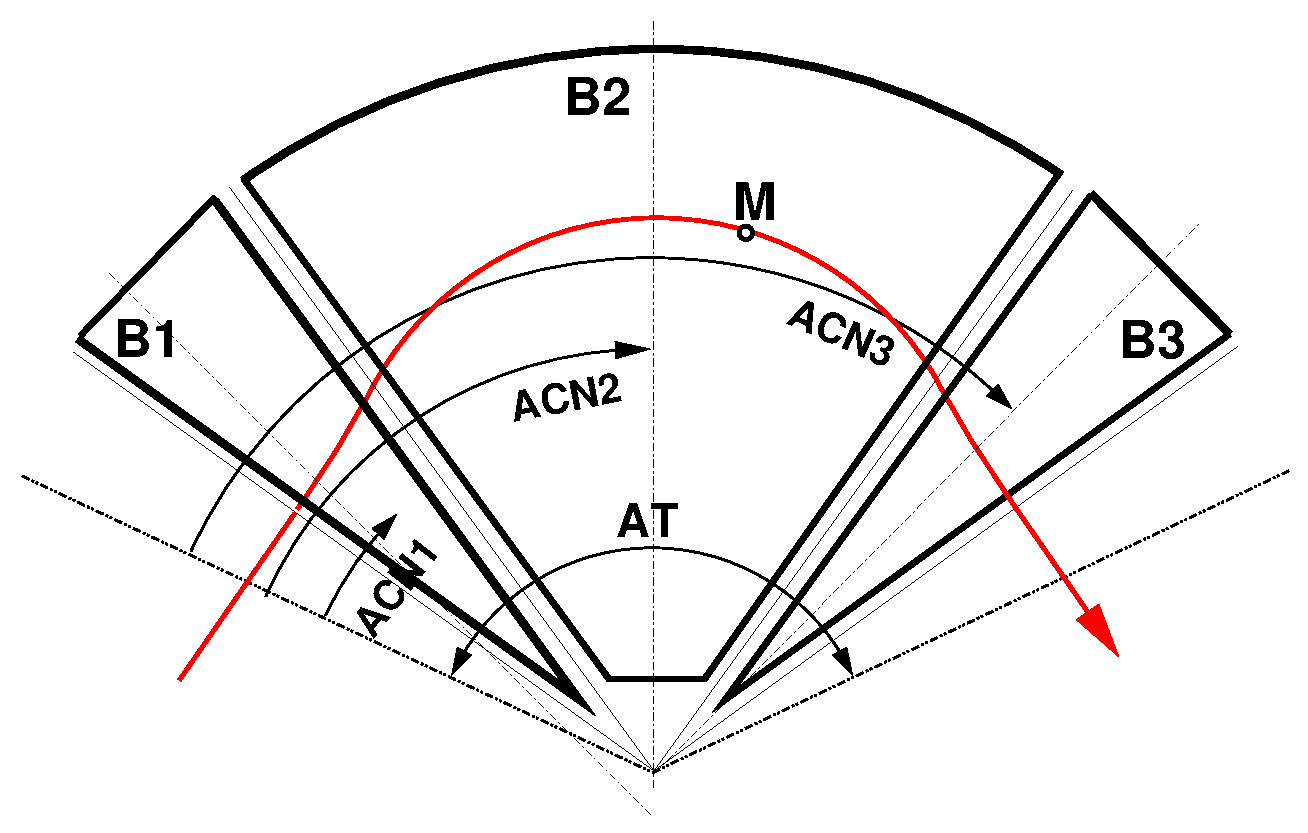
\includegraphics[width=8.5cm]{ffagTriplet.eps}  
 \caption{ \label{figDFD}
Definition of a dipole triplet using  the \textsl{DIPOLES} or  \textsl{FFAG}  procedures. 
}
  \end{center}
\end{figure}





\paragraph{Calculation of the fringe field coefficient} 

\noindent In a dipole, with  each EFB a realistic extent of the fringe field, $g $, 
is associated and a fringe field coefficient $ F $ is calculated. 


\bigskip

\noindent$ F $ is an exponential type fringe field (Fig.~\ref{fig11}, page~\pageref{fig11}) 
given by~\cite{Biblio12}     %%% [12]

$$ F = \frac{1 }{ 1+ \exp P(d)} $$
%
 wherein $ d $ is the distance to the EFB and depends on $(R,\theta)$, and 

$$
    P(d) = C_0
       +C_1 \left(  \dfrac{d }{ g } \right) 
       +C_2 \left( \dfrac{d }{ g } \right)^2 
       + C_3 \left( \dfrac{d }{ g } \right)^3 
       +C_4 \left( \dfrac{d }{ g } \right)^4 
       + C_5 \left(\dfrac{d }{ g } \right)^5 $$

\noindent In addition,   $g$ is made dependent  of $R$ 
(a way to simulate the effect of variable gap size on field fall-off), 
under the form 

$$ g(R) = g_0 \, (RM/R)^{\kappa}  $$

This dependence is accounted for rigorously if the interpolation method is 
used, to zero order (derivatives of $g(R)$ are not considered) if the analytic method is used. 

\smallskip

\noindent Let $ F_E $ (respectively $ F_S$)  be the fringe field
coefficient attached to the entrance (respectively exit) EFB~; at any position on  a 
trajectory the resulting value of the fringe field coefficient is taken to be 

\begin{equation}
\label{EqFFdips}
  \mathcal{F}_i(R,\theta) = F_E  \ast  F_S 
\end{equation}



\paragraph{Calculation of the full field from all $N$ dipoles \label{FFatAP}}

 
\noindent Now, accounting for   $N$ neighboring dipoles in an $N$-tuple,  the mid-plane field  and field derivatives  
are  obtained by addition of  the  contributions of the $N$ dipoles taken separately, namely

\begin{eqnarray}
\label{EqSumB}
\Bz(R,\theta) &=&  \sum_{i=1,N} \Bz_i(R,\theta)   =  \sum_{i=1,N} \Bz_{0,i} \, \mathcal{F}_i(R,\theta) 
\,  \mathcal{R}_i(r)  \nonumber \\
\frac{\partial^{ k+l}\vec \Bz(R,\theta) }{ \partial \theta^k\partial r^l} &=&  \sum_{i=1,N} 
\frac{\partial^{ k+l}\vec \Bz_i(R,\theta) }{ \partial \theta^k\partial r^l} 
\end{eqnarray}

\noindent with $\mathcal{R}_i(R)$ as defined in Eq.~\ref{EqFieldDipoles}. 
Note that, in doing so it is not meant that field superposition  does apply 
in reality, it is just meant to provide the possibility 
of obtaining a realistic  field shape, that would for instance closely match (using appropriate $C_0-C_5$ sets 
of coefficients) 3-D  field simulations obtained from magnet codes. 


\bigskip




\paragraph{Calculation of the  mid-plane field derivatives}

\noindent Two  methods have been implemented to calculate the field derivatives in the median 
plane (Eq.~\ref{EqSumB}), based on 
 either analytical expressions derived from the magnet geometrical description,  or  classical numerical interpolation. 
 
\noindent The first method has the merit of insuring best symplecticity in principle and fastest tracking. 
The interest of the second method is in its  facilitating possible  changes in 
  the mid-plane magnetic field model $\Bz(R,\theta)$, for instance if simulations of shims, defects, 
or special $R, \theta$  field dependence need to be introduced. 



\bigskip

\noindent {\it Analytical method~: }

\bigskip

\noindent The  starting ingredients are, on the one hand distances to the EFBs,  

$$d(R,\theta)=\sqrt{(x(R,\theta)-x_{0}(R,\theta))^2+(y(R,\theta)-y_{0}(R,\theta))^2}$$

\noindent to be computed for the two cases $d_{\textrm{Entrance}}$, $d_{\textrm{Exit}}$, and 
on the other hand the expressions of the coordinates of particle position $M$ and its projection $P$ on 
the EFB in terms of the magnet geometrical parameters, namely 

\begin{eqnarray}
x(R,\theta)&=&\cos (ACN-\theta)-RM   \nonumber \\[-1ex]
y(R,\theta)&=&R\sin (ACN-\theta)   \nonumber \\[-1ex]
x_P(R,\theta)&=&\sin(u)\:  (y(R,\theta) - y_b)/2 + x_b\:  \sin^2(u) + x(R,\theta)\:  \cos^2(u)   \nonumber \\[-1ex]
y_P(R,\theta)&=&\sin(u)\: (x(R,\theta) - x_b)/2 + y_b\:  \cos^2(u) + y(R,\theta) \: \sin^2(u)   \nonumber 
\end{eqnarray}

\noindent with $x_b,~y_b,~u$ parameters drawn from the  magnet geometry (sector angle, wedge angle, face curvatures, etc.). 

\noindent These ingredients allow calculating  the derivatives 
$\frac{\partial^{ u+v}x(R,\theta)}{ \partial \theta^u\partial r^v}\:,$ 
$\:\: \frac{\partial^{ u+v}y(R,\theta)}{ \partial \theta^u\partial r^v}\:,$ 
$\:\:\frac{\partial^{ u+v}x_0(R,\theta)}{ \partial \theta^u\partial r^v}\:,$ 
$\:\:\frac{\partial^{ u+v}y_0(R,\theta)}{ \partial \theta^u\partial r^v}\:,$ 
which, in turn,  intervene in the derivatives of the compound functions 
$\frac{\partial^{ u+v}F(R,\theta)}{ \partial \theta^u\partial r^v}\:,$ 
$\:\:\frac{\partial^{ u+v}p(R,\theta)}{ \partial \theta^u\partial r^v}\:,$ 
$\:\:\frac{\partial^{ u+v}d(R,\theta)}{ \partial \theta^u\partial r^v}$. 


\bigskip

\noindent { \it Interpolation method~:  \label{CalcMidPlaneFieldInterpol}}

\bigskip

\noindent The expression $\Bz(R,\theta)$ in Eq.~\ref{EqSumB} is, in this case, 
computed at  the $n\times n$ nodes  ($n=3$ or $5$ in practice)  
of a ``flying'' interpolation grid in the median plane centered on the projection $m_0$ of 
the actual particle position $M_0$ as schemed 
in Fig.~\ref{FigGrid}. A polynomial interpolation is involved, of the form 

$$\Bz(R,\theta) = A_{00} + A_{10}\theta + A_{01}r + A_{20}\theta^2 + A_{11}\theta r + A_{02}r^2 $$

\noindent  that yields the requested   derivatives, using 
$$	A_{kl} = \frac{1 }{ k!l!}\,  \frac{\partial^{ k+l}B }{ \partial \theta^k\partial r^l} $$

\noindent Note that, the source code contains the explicit analytical 
expressions of the coefficients $A_{kl}$ solutions of the normal 
equations, so that the operation {\it is not}   CPU time consuming. 

\begin{figure}[h]
 \begin{center}
\includegraphics*[bbllx=30,bblly=150,bburx=590,bbury=400,width=8.2cm,height=4.3cm]{grid.eps}
  \caption{ \small     \label{FigGrid}
Interpolation method.  
$m_0$ and $m_1$ are the projections in the median plane of particle positions $M_0$ and $M_1$  separated 
by one integration step $\delta s$. 
}
  \end{center}
\end{figure}


\bigskip

\paragraph{Extrapolation Off Median Plane} 

\noindent From the vector field $ \vec  B $ and  derivatives in the median plane, 
first a transformation from polar to Cartesian coordinates is 
performed, following eqs (\ref{eq2-4-8} or \ref{eq2-4-9}), then,  extrapolation off median plane is 
performed by means of Taylor expansions, following the procedure described in section~\ref{sec2.3.2}. 




\bigskip

\paragraph{Sharp edge} 

\noindent Sharp edge field fall-off at a field boundary  can only be simulated if the following conditions are fulfilled~: 

- entrance (resp. exit)  field boundary  coincides with entrance (resp. exit) 
dipole limit (it means in particular, see Fig.~\ref{fig9},  
$\omega^+= ACENT$ (resp. $\omega^- = -(AT-ACENT)$), 
together with $\theta=0$ at entrance (resp. exit) EFBs), 

- analytical method for calculation of the  mid-plane field derivatives is used. 








\newpage

\subsubsection*{DODECAPO~: \DODECAPOTitl\  (Fig.\protect~\ref{fig19})} \label{DODECAPO}  \index{DODECAPO|textbf}
\medskip


 The meaning of parameters for \textsl{DODECAPO}  is the same as for \textsl{QUADRUPO}. 
%\bigskip

\noindent In fringe field regions the magnetic field $ \vec  B(X,Y,Z) $ and
its derivatives up to fourth order are derived from the scalar potential approximated to 
the 6th order in $ Y $ and $ Z $ 

\begin{align*}
	V(X,Y,Z) &   = G \left(Y^4- \dfrac{10 }{ 3} Y^2Z^2+Z^4 \right) YZ  \\
	\text{with } G_0 &   =  \dfrac{ B_0 }{ R^5_0} 
\end{align*}

\noindent Outside fringe field regions, or everywhere in sharp edge dodecapole
($ \lambda_ E=\lambda_ S=0$) , $ \vec  B(X,Y,Z) $ in the magnet is given by 

\begin{align*}
	B_X &   =   0 \\
	B_Y &   =    G_0(5Y^4-10Y^2Z^2+Z^4)Z \\
	B_Z &   = G_0(Y^4-10Y^2Z^2+5Z^4)Y  
\end{align*}
\vfill

%%%%%%%%%%%%%%figure%%%%%%%%%%%%%%
\begin{figure}[H]
%\vspace{12 truecm}
%%%Figure 19
\centerline{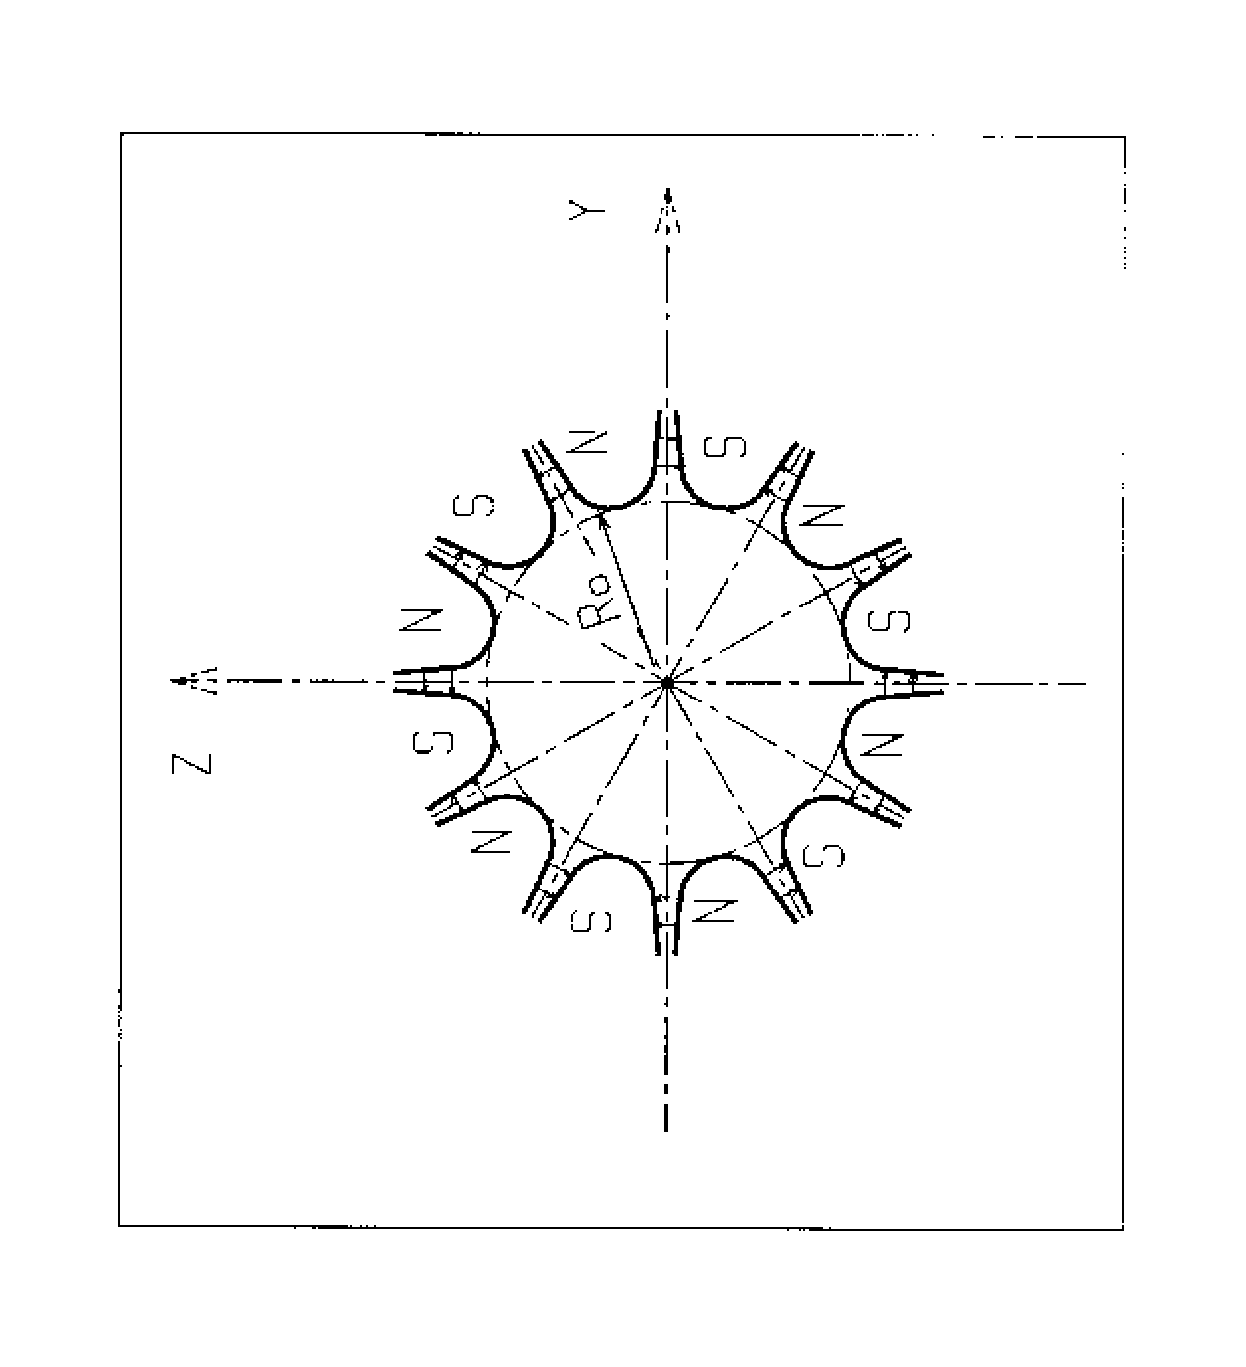
\includegraphics[width=12cm,angle=-90]{Fig19.ps}}
\caption{\label{fig19}Dodecapole magnet}
\end{figure}
\vfill

\newpage
\subsubsection*{DRIFT or ESL~: \DRIFTTitl}\label{ESL}\label{DRIFT}\index{DRIFT|textbf}\index{ESL|textbf}
\medskip

\textsl{DRIFT} or \textsl{ESL} allow introduction of a drift space with length $ \XL $ with 
positive or negative sign, anywhere in a structure.  The associated equations 
of motion are (Fig.~\ref{fig23})   

\begin{align*}
	Y_2 &   =    Y_1+\XL \ast \text{tg} T  \\ 
	Z_2 &   =   Z_1 + \dfrac{\XL}{\cos  T}\,  \text{tg} P  \\
	SAR_2 &   =  SAR_1+ \dfrac{\XL }{\cos  T  \ast \cos  P}  
\end{align*}
\vfill

%%%%%%%%%%%%%%figure%%%%%%%%%%%%%%
\begin{figure}[H]
%\vspace{15 truecm}
%%%Figure 23
\centerline{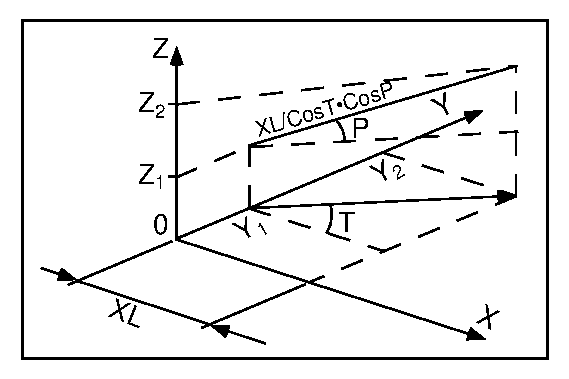
\includegraphics[width=15cm]{Fig23.ps}}
\caption{\label{fig23}Transfer of particles in a drift space.}
\end{figure}
\vfill

\newpage
\subsubsection*{EBMULT~: \EBMULTTitl}\label{EBMULT} \index{EBMULT|textbf}
\medskip

\noindent\textsl{EBMULT} simulates an electro-magnetic multipole, by addition of
electric $ (\vec  E) $ and magnetic $ (\vec  B) $ multipole components (dipole to 20-pole). 
$\vec  E $ and its derivatives 
$ \dfrac{\partial^{ i+j+k} \vec  E }{ \partial X^i\partial Y^j\partial Z^k} $ 
($i+j+k \le 4$) are derived 
from the general expression of the multipole scalar potential (eq.~\ref{eq2-3-5}), followed by a 
$ \frac{\pi }{2n} $ rotation  ($n= $ pole order), 
as described in section~\ref{sec2.5.3} (see also \textsl{ELMULT\index{ELMULT}}). $ \vec  B $ and its
derivatives are derived from the same general potential, as described in section~\ref{sec2.3.5} 
(see also \textsl{MULTIPOL\index{MULTIPOL}}). 

\noindent The entrance and exit fringe fields of the $ \vec  E $ and $ \vec  B$ components are treated 
separately, in the same way as described under \textsl{ELMULT\index{ELMULT}} 
 and \textsl{MULTIPOL\index{MULTIPOL}},
for each one of these two fields. Wedge angle correction is applied in sharp edge field model if $ \vec  B1$ is non zero, as in \textsl{MULTIPOL}. Any of the $ \vec  E $ or $ \vec  B $ multipole field
component can be rotated independently of the others. 

\noindent Use \textsl{PARTICUL\index{PARTICUL}} prior to \textsl{EBMULT}, for the 
 definition of  particle mass and charge.
\vfill

%%%%%%%%%%%%%%figure%%%%%%%%%%%%%%
\begin{figure}[H]
%\vspace{15 truecm}
%%%Figure 20
\centerline{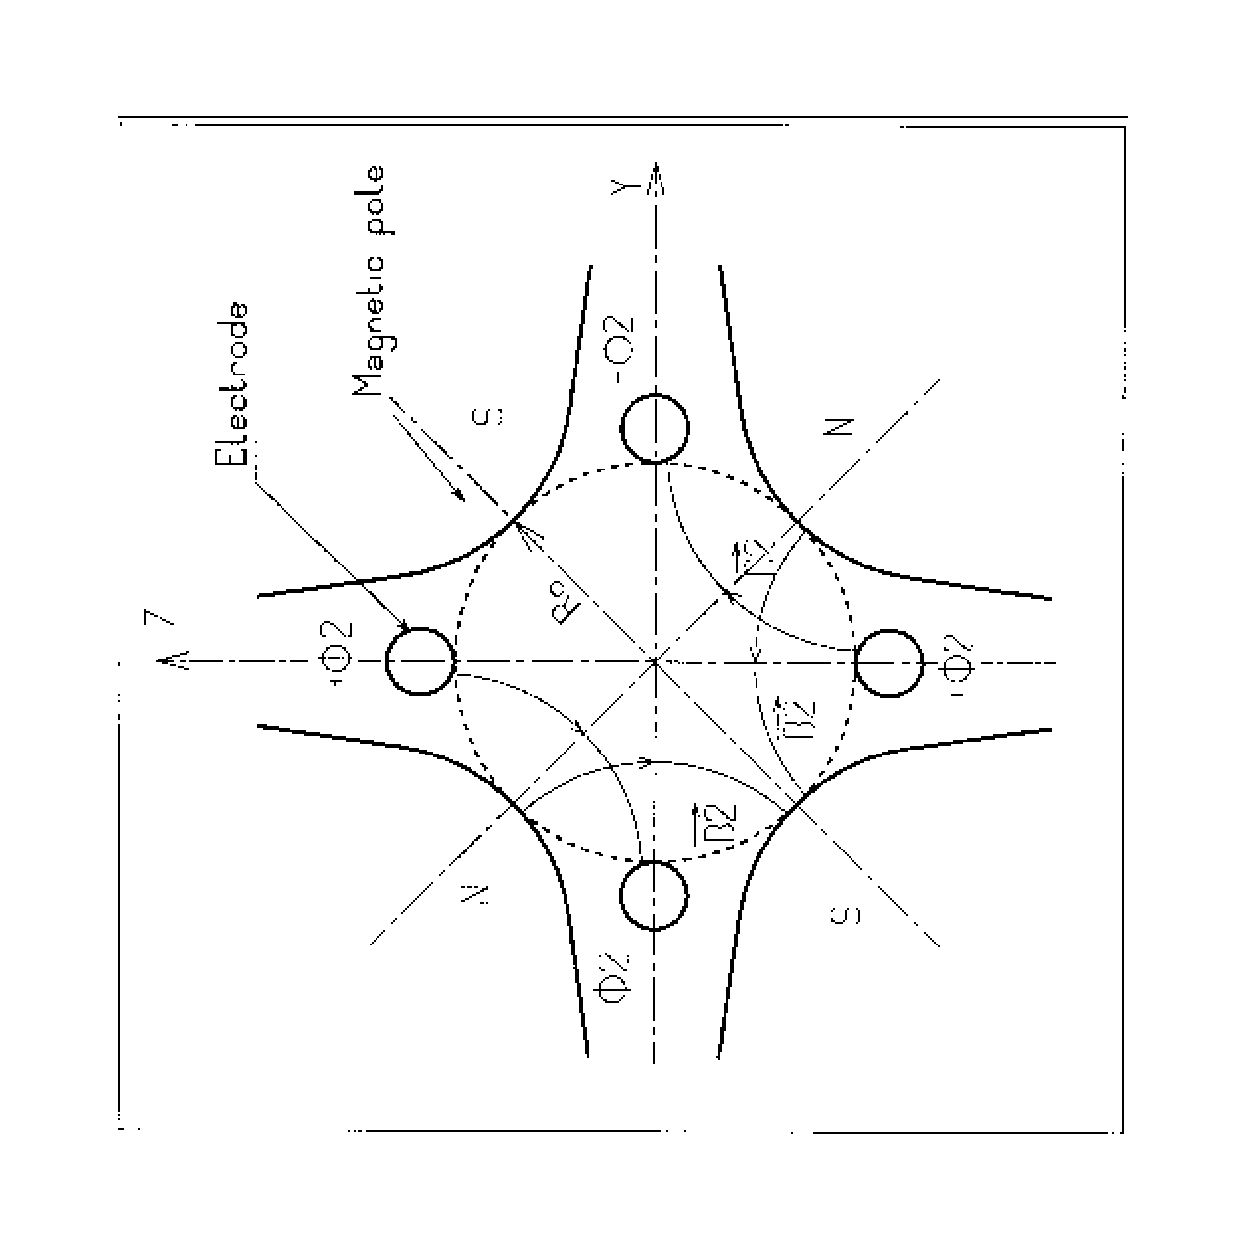
\includegraphics[height=12cm,angle=-90]{Fig20.ps}}
\hangcaption[Fig20]{\label{fig20}An example of $ \vec  E$, $\vec  B $ multipole~: 
           the achromatic quadrupole  \\  
          (known for its allowing null second order chromatic aberrations~\protect\cite{Biblio14}).}
\end{figure}

\newpage

\subsubsection*{EL2TUB~: \ELTwoTUBTitl} \label{EL2TUB} \index{EL2TUB|textbf}
\medskip

The lens is cylindrically symmetric about the $ X $-axis. 

\noindent The length and potential of the first (resp. second) electrode 
are $ X1 $ and $ V1 $ ($ X2 $ and $ V2$).   The distance between the two 
electrodes is $ D$,   and their inner radius is $ R_0 $ (Fig.~\ref{fig22}).   
$X$-axis  cylindrical symmetry is assumed. The model for the electrostatic potential 
along the axis is~\cite{Biblio16}     %% [16]

 \begin{alignat*}{2}
	 V(X) &   = \dfrac{ V_2-V_1}{2} \: \text{th}\,
	            \dfrac{\omega x }{ R_0} 
	             \left[+ \dfrac{V_1+V_2 }{ 2} \right] 
	      & \qquad \text{if }  D & =0\\
	V(X) &  =  \dfrac{ V_2-V_1 }{ 2}\: \dfrac{1}{ 2\omega D} \: \ell n\,
	           \dfrac{\text{ch}\, \omega\,    \dfrac{x+D }{ R_0} }%
	           {\text{ch} \,\omega \,\dfrac{x-D }{ R_0}}
	           \left[+ \dfrac{V_1+V_2 }{ 2} \right]
	            & \qquad \text{if }  D &  \not= 0 
 \end{alignat*}
%
($ x $ = distance from half-way between the electrodes~;
$\omega$  =  1.318~; th =  hyperbolic tangent~; ch  =  hyperbolic cosine)
from which the field $ \vec  E(X,Y,Z) $ and its derivatives are derived following the 
procedure described in section~\ref{sec2.5.2}  (note that they don't 
depend on the constant term $ \left[\dfrac{V_1+V_2 }{ 2} \right] $ which
disappears when differentiating). 

\noindent Use \textsl{PARTICUL\index{PARTICUL}} prior to \textsl{EL2TUB}, for the
 definition of  particle mass and charge.

\vfill

%%%%%%%%%%%%%%figure%%%%%%%%%%%%%%
\begin{figure}[H]
%\vspace{13 truecm}
%%%Figure 22
\centerline{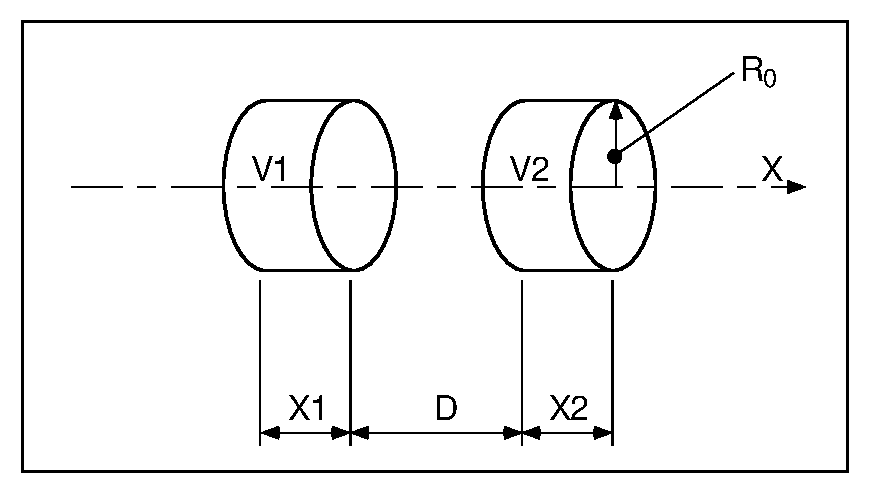
\includegraphics[width=14cm]{Fig22.ps}}
\caption{\CapELtwoTUB \label{fig22}}
\end{figure}

\vfill

\newpage

\subsubsection*{ELMIR~: \ELMIRTitl }\label{ELMIR}\index{ELMIR|textbf}
\medskip

The device works as  mirror or lens, horizontal or vertical. 
It is made of $N$ 2-plate electrodes and has mid-plane symmetry.  
\bigskip

\noindent Electrode lengths are  $ L\!1 $, $ L\!2 $, ...,   $ L\!N$. $D$ is the  mirror/lens gap. 
The model for the $Y$-independent electrostatic potential is (after Ref.~\cite[p.412]{Karets}) 
$$ V(X,Z) = 
   \sum_{i=2}^{N} \dfrac{V{i}-V{i\!-\!\textrm{\footnotesize 1}} }{ \pi} 
     \arctan\dfrac{\sinh(\pi ( X - X{i\!-\!\textrm{\footnotesize 1}})/D)}{\cos(\pi Z/D)}   
$$
where $V\!i$ are the potential at the $N$ electrodes (and normally $V\!1=0$ refers to 
the incident beam energy),   $X\!i$ are the  locations of the slits, $ X $ is the distance 
from the origin taken at the first slit (located at $X\!1 \equiv 0$ between the first and 
second electrodes).  
 From $V(X,Z) $ the field $ \vec  E(X,Y,Z) $ and derivatives are deduced following the procedure 
described in section~\ref{sec2.5.3}~(page~\pageref{sec2.5.3}).  

\noindent The total X-extent of the mirror/lens is $L = \sum_{i=1}^N L\!i$.

\noindent In the mirror mode ({\it i.e.}, option flag $MT=11$ for vertical mid-plane  or $12$ 
for horizontal mid-plane) stepwise integration starts 
at $X=-L\!1$ (entrance of the first electrode) and terminates either when back to   $X=-L\!1$  
or when  reaching $ X=L-L\!1$ (end of the $N-th$ electrode). 
In the latter case particles  are stopped  with their index
 $I\!E\!X$ set to $-8$ (see section~\ref{sec4.6.6} on page~\pageref{sec4.6.6}). 
Normally $X\!1$ should   exceed  $3D$ (possibly sensibly, 
so that $V(X<X\!1)$   have negligible effect in terms of trajectory behavior).  

\noindent In the lens mode ({\it i.e.}, option flag $MT=21$ for vertical mid-plane  or $22$
for horizontal mid-plane) stepwise integration starts
at $X=-L\!1$ (entrance of the first electrode) and terminates either when reaching $ X=L-L\!1$ (end of the $N-th$ electrode) 
or when the particle deflection exceeds $\pi/2$. In the latter case the particle is stopped  with their index
 $I\!E\!X$ set to $-3$. 
 
\bigskip

\noindent Use \textsl{PARTICUL\index{PARTICUL}} prior to \textsl{ELMIR}, for the
 definition of particle mass and charge.

\bigskip
\vfill

%%%%%%%%%%%%%%figure%%%%%%%%%%%%%%
\begin{figure}[H]
\centerline{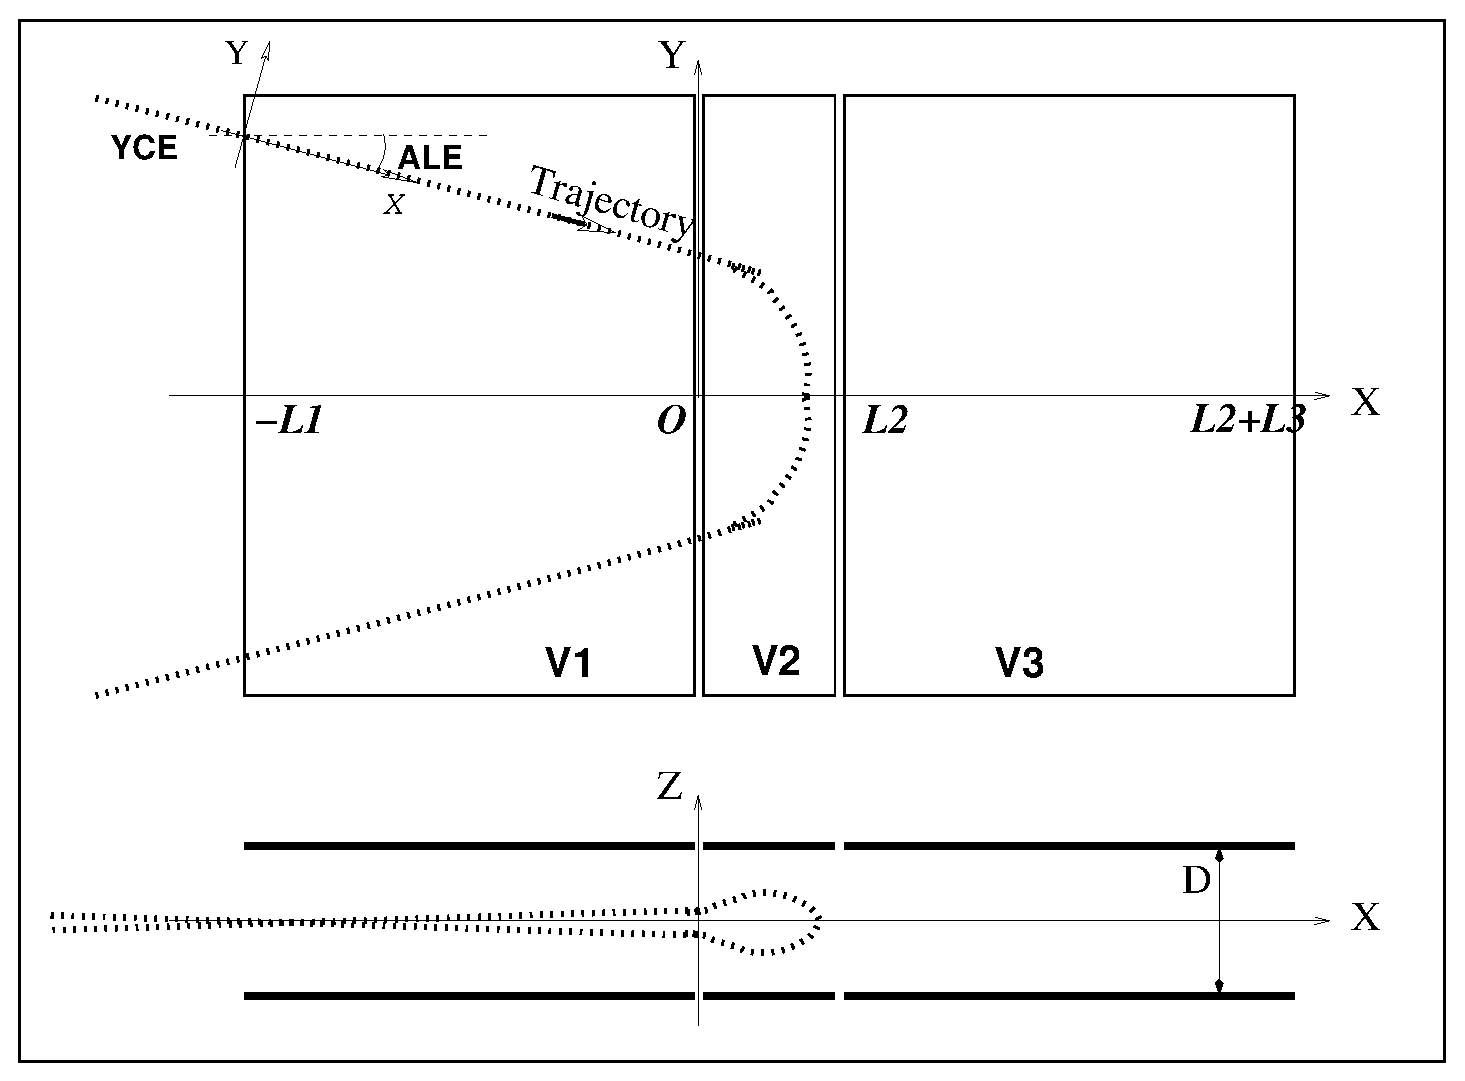
\includegraphics[height=8cm]{FigELMIR.eps}}
\hangcaption{\label{figELMIR} \CapELMIR}
\end{figure}

\vfill

\newpage

\subsubsection*{ELMIRC~: \ELMIRCTitl~\cite{Karets}}\label{ELMIRC}\index{ELMIRC|textbf}
\medskip

The device works as  mirror or lens, horizontal or vertical. 
It is made of $N$ 2-plate electrodes and has mid-plane 
symmetry\footnote{NOTE~: in the present version of the code, the sole horizontal mirror mode 
 is operational, and $N$ is limited to 3.}. 
\bigskip

\noindent Electrode  slits are circular, concentric with  radii  $ R1 $, $ R2 $, ...,   
$ R{\textrm{\footnotesize N-1}}$, 
$D$ is the  mirror/lens gap. The model for the mid-plane ($Z=0$) radial electrostatic potential  
is (after Ref.~\cite[p.443]{Karets})
$$ V(r) = 
   \sum_{i=2}^{N} \dfrac{V{i}-V{i\!-\!\textrm{\footnotesize 1}} }{ \pi} 
     \arctan \left( \sinh \dfrac{ \pi ( r - R{i\!-\!\textrm{\footnotesize 1}})}{D} \right)  
%    \dfrac{V-V\!A }{ \pi} \arctan \sinh \dfrac{\pi (r -R1)}{D} + 
%  \dfrac{V\!B - V }{ \pi} \arctan \sinh \dfrac{\pi (r -R2)}{D} 
$$
where $V\!i$ are the potential at the $N$ electrodes (and normally $V\!1=0$ refers to
the incident beam energy). $r$ is the current radius. 

 The mid-plane field $ \vec  E(r) $ and its $r$-derivatives are first derived by differentiation, then 
$ \vec  E(r,Z) $ and  derivatives are obtained from Taylor expansions and Maxwell relations. 
Eventually a transformation to the rotating frame provides $\vec  E(X,Y,Z)$ 
 and  derivatives as involved in eq.~\ref{eq2-2-12}. 


\noindent Stepwise integration starts at entrance (defined by $R\!E, T\!E$) of the first electrode 
and terminates when rotation of the reference  rotating frame  $(RM,X,Y)$ has reached the value AT. 
Normally, $R1-R\!E$ and $R1-R\!S$ should both  exceed  $3D$ (possibly sensibly, 
so that $V(r<R\!E)$ and $V(r<R\!S)$  have negligible effect in terms of trajectory tails).  

Positioning of the element is performed by means of \textsl{KPOS} (see section~\ref{sec4.6.2}). 

\bigskip

\noindent Use \textsl{PARTICUL\index{PARTICUL}} prior to \textsl{ELMIRC}, for the
 definition of particle mass and charge.

\vfill

%%%%%%%%%%%%%%figure%%%%%%%%%%%%%%
\begin{figure}[H]
\centerline{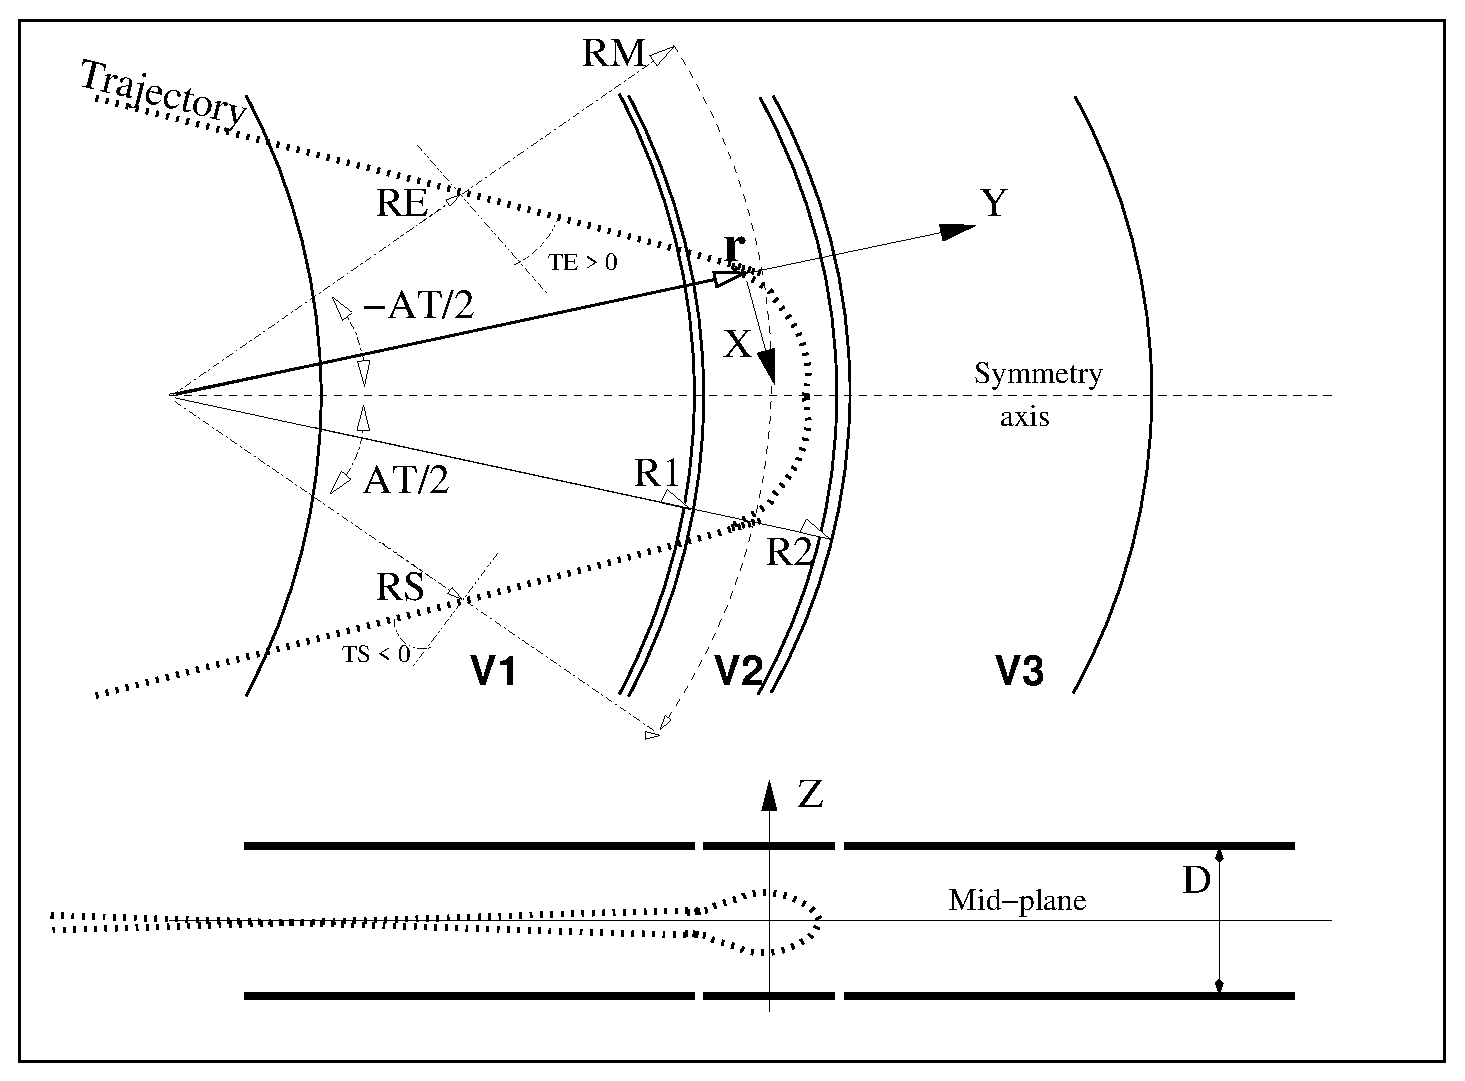
\includegraphics[height=10cm]{FigELMIRC.eps}}
\caption{\label{figELMIRC} \CapELMIRC}
\end{figure}

\vfill


\newpage

\subsubsection*{ELMULT~: \ELMULTTitl} \label{ELMULT}\index{ELMULT|textbf}
\medskip

The simulation of multipolar electric  field $ \vec  M_E $ proceeds by addition of 
the dipolar $ (\vec  E1) $,  quadrupolar ($ \vec  E2 $), sextupolar ($ \vec  E3 $), 
etc.,  up to 20-polar $ (\vec  E10) $ components, and of their derivatives up to fourth 
order, following

\begin{align*}
	\vec  M_E & = \vec  E1 + \vec  E2 + \vec  E3 + ~...~ + \vec  E10 \\
	\dfrac{ \partial\vec  M_E }{ \partial X}  
	          & =  \dfrac{ \partial\vec  E1 }{ \partial X} +
	               \dfrac{\partial\vec  E2 }{ \partial X} + 
	               \dfrac{\partial\vec  E3 }{ \partial X} +
	                         ~...~ +
	               \dfrac{\partial\vec  E10 }{ \partial X}  \\
	\dfrac{ \partial^ 2M_E}{ \partial X\partial Z} 
	          &   = \dfrac{\partial^ 2\vec  E1 }{ \partial X\partial Z} +
	               \dfrac{\partial^ 2\vec  E2 }{\partial X\partial Z} + 
	               \dfrac{\partial^ 2\vec  E3 }{ \partial X\partial Z} +
                                 ~...~ +
	               \dfrac{\partial^ 2\vec  E10 }{ \partial X\partial Z}  \\
	   \text{etc.} &
\end{align*}

\noindent The independent components $ \vec  E1 $ to $ \vec  E10 $ and their
derivatives up to the second order are calculated by differentiating the general multipole potential 
 given  in eq.~\ref{eq2-3-5} (page~\pageref{eq2-3-5}), followed by 
  a $ \frac{\pi }{ 2n} $ rotation about the $ X$-axis, so
that the so defined right electric multipole of order $ n$,  and of 
strength~\cite{Biblio14, Biblio15}   %% [14, 15]

$$ K_n = \dfrac{1 }{ 2}\, \dfrac{\gamma }{ \gamma^ 2-1}\, \dfrac{V_ n }{ R^n_0} $$
%
$ (V_ n $ = potential at the electrode, $ R_0 $ = radius at pole tip, 
$\gamma$  = relativistic Lorentz factor of the particle) has the same focusing effect 
than the right magnetic multipole of order $ n $ and strength
 $ K_n= \dfrac{B_n }{ R^{n-1}_0 \Br} $ 
$ (B_n $ = field at pole tip, $ \Br $ = particle rigidity, see \textsl{MULTIPOL\index{MULTIPOL}}). 

\noindent Such $ \dfrac{\pi }{ 2n} $ rotation of the multipole components is
obtained following the procedure described in section~\ref{sec2.5.3}.  
\bigskip

\noindent The entrance and exit fringe fields are treated separately.  They
are characterized by the integration zone $ X_E $ at entrance and $ X_S $ at exit,
as for \textsl{QUADRUPO\index{QUADRUPO}}, and by the extent $ \lambda_ E $ at entrance, $\lambda_ S $ 
at exit. The fringe field extents for the dipole component are $ \lambda_ E $
and $ \lambda_ S $. The fringe field for the quadrupolar (sextupolar,  ..., 
 20-polar) component is given by a coefficient $ E_2 $ 
 ($E_3$, ..., $E_{10}$)   at entrance, and $ S_2 $ ($ S_3$, ..., $S_{10}$)   at exit, 
 such that the fringe field extent is $ \lambda_ E\ast E_2$  
 ($\lambda_ E\ast E_3$, ..., $\lambda_ E\ast E_{10}$)  at 
entrance and $ \lambda_ S\ast S_2 $  ($\lambda_ S\ast S_3$, ..., $\lambda_ S\ast S_{10}$) 
 at exit.  
\bigskip

\noindent If $ \lambda_ E=0 $  ($\lambda_ S=0$)  the multipole lens is
considered to have a sharp edge field at entrance (exit), and then, 
$ X_E \ (X_S) $ is forced to zero (for the mere purpose of saving computing time).  
\bigskip

\noindent If $ E_i=0 $  ($S_i=0$) ($i=2,\, 10$), the entrance (exit) fringe field for
multipole component $ i $ is considered as a sharp edge field.  
\bigskip

\noindent Overlapping of fringe fields inside the element is treated
separately for each component, in the way described in \textsl{QUADRUPO\index{QUADRUPO}}. 

\noindent Moreover, any multipole component $ \vec  Ei $ can be rotated
independently by an angle $ RXi $ around the longitudinal $ X$-axis, for the simulation of 
positioning defects, as well as skewed lenses. 

\noindent Use \textsl{PARTICUL\index{PARTICUL}} prior to \textsl{ELMULT}, for the
 definition of particle mass and charge.

\vfill

%%%%%%%%%%%%%%figure%%%%%%%%%%%%%%
\begin{figure}[H]
%\vspace{19 truecm}
%%%Figure 21
\centerline{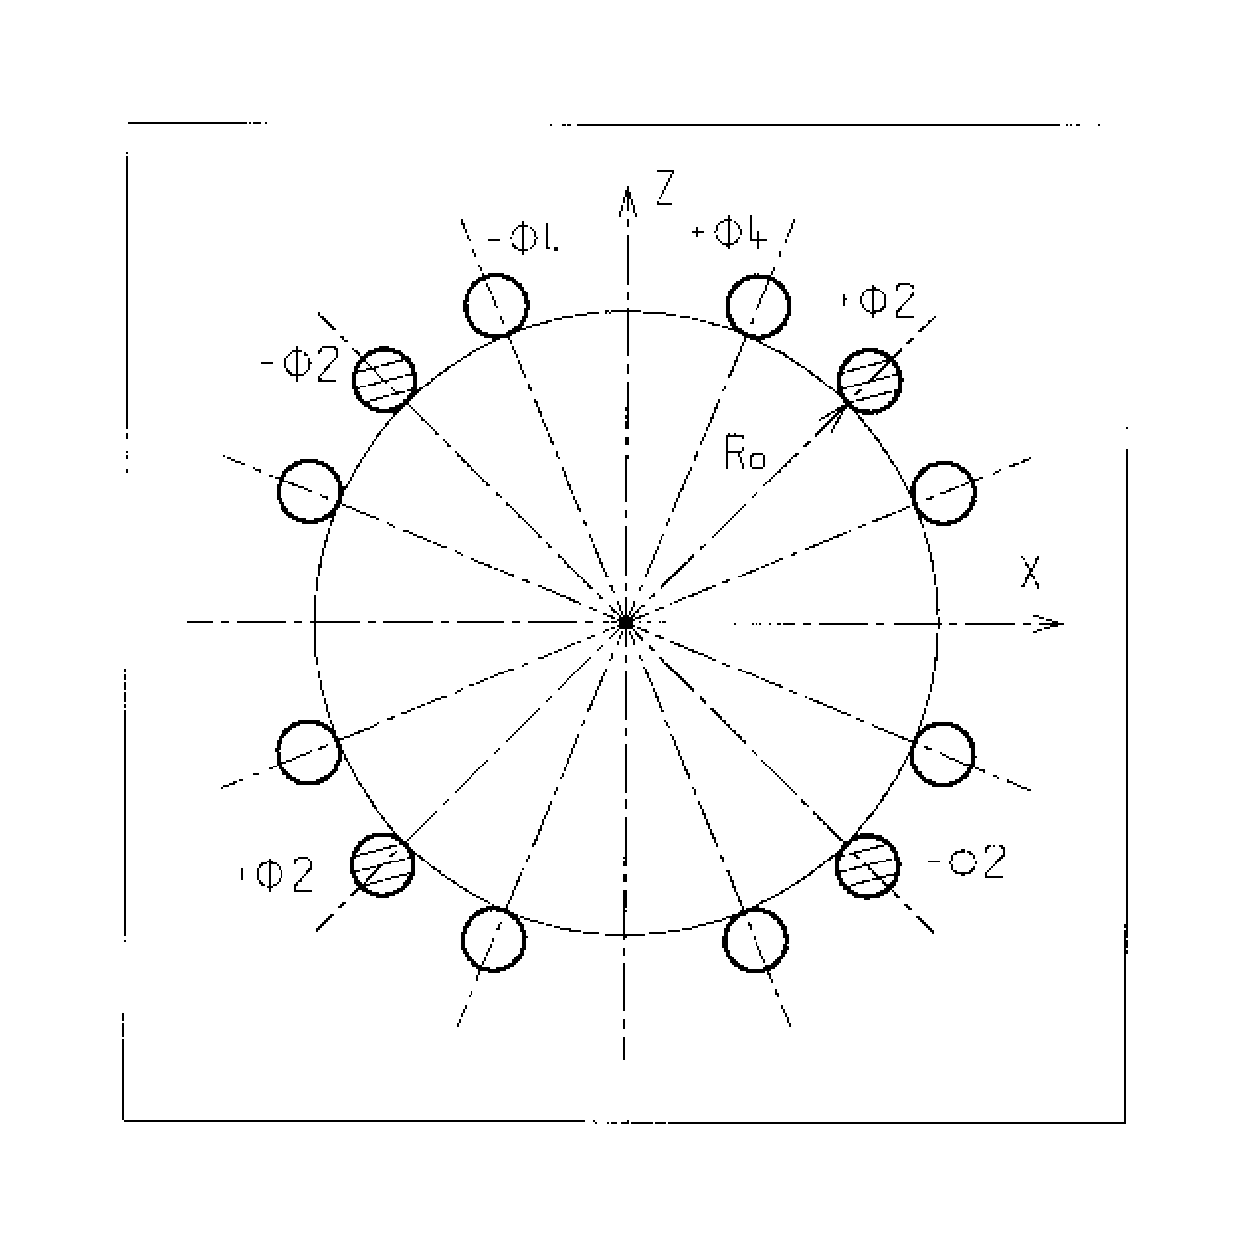
\includegraphics[width=14cm]{Fig21.ps}}
{\setlength{\captionwidth}{10cm}
\hangcaption[Fig21]{\label{fig21}An electric multipole combining skew-quadrupole $ (\vec  E2 \ne \vec 0,~ \vec R2 = \pi/4)$ and  
skew-octupole $ (\vec  E4 \ne \vec 0,~ \vec R4 = \pi/8) $ components 
 ($\vec E1=\vec  E3=\vec  E5= \ ...\ = \vec  E10= \vec 0 $)~\protect\cite{Biblio15}. }   
}\end{figure}
\vfill










\newpage

\subsubsection*{ELREVOL~: \ELREVOLTitl}  \label{ELREVOL}\index{ELREVOL|textbf}
\medskip

\textsl{ELREVOL}  reads a 1-D axial field map from a storage data file,
whose content must fit the following \FORTRAN reading sequence  


{\footnotesize
\begin{verbatim}
	      OPEN (UNIT = NL, FILE = FNAME, STATUS = `OLD' [,FORM='UNFORMATTED'])
	      DO 1 I=1, IX
	         IF (BINARY) THEN 
	            READ(NL) X(I), EX(I)
	         ELSE
	            READ(NL,*) X(I), EX(I)
	         ENDIF 
        1     CONTINUE
\end{verbatim}}%% 
\bigskip

\noindent where $IX$ is the number of nodes along the (symmetry) $X$-axis, $X(I)$ their 
coordinates, and $EX(I)$ the values of the $X$ component of the field. $EX$ is 
normalized with \textsl{ENORM} prior to ray-tracing. As well the longitudinal coordinate  X is normalized with 
a  \textsl{XNORM} coefficient (usefull to convert to centimeters, the working units in  \zgoubi. 


\bigskip

\noindent$X$-cylindrical symmetry is assumed, resulting in $EY$
and $EZ$ taken to be zero on axis. $ \vec  E(X,Y,Z) $ and its derivatives along a particle
trajectory are calculated by means of a 5-points polynomial fit followed by second 
order off-axis Taylor series extrapolation (see sections~\ref{sec2.5.1} and \ref{sec2.6}).  
\bigskip

\noindent Entrance and/or exit integration boundaries may be defined in the same way 
as in \textsl{CARTEMES\index{CARTEMES}} by means of the flag $ID$ and coefficients  
$A$, $B$, $C$, $A'$, $B'$, $C'$.  
\bigskip

\noindent Use \textsl{PARTICUL\index{PARTICUL}} prior to \textsl{ELREVOL}, for the
 definition of particle mass and charge.



\newpage

\subsubsection*{EMMA~: \EMMATitl} \label{EMMA} \index{EMMA}
\medskip

 \textsl{EMMA} is dedicated to the reading and treatment of 2-D or 
3-D Cartesian or cylindrical mesh field maps as  delivered by the
\textsl{TOSCA}  magnet computer code standard output.

\bigskip

That part of the manual to be provisionned...

\medskip

\noindent where, $IX$ ($JY$, $KZ$)  is   the number of longitudinal 
(transverse horizontal, vertical) nodes of the 3-D uniform mesh. For binary files, 
FNAME must begin with  \mbox{`B\_'} or  \mbox{`b\_'}, a flag  `BINARY' will thus be set to `.TRUE.'.  

A flag \textsl{MOD} determines wether Cartesian or Z-axis cylindrical mesh is used. \textsl{MOD} can 
take various values depending also on the map data file formatting. (To be documented - see FORTRAN 
subroutine FMAPW and its entries FMAPR, FMAPR2.)

\bigskip

\noindent The field $ \vec  B=(B_X,B_Y,B_Z) $ is normalized by means of 
\textsl{BNORM} in a similar way as in \textsl{CARTEMES\index{CARTEMES}}.  
 As well the  coordinates  X (and Y, Z with 3-D field maps) is normalized with 
a  \textsl{X-[Y-,Z-]NORM} coefficient (usefull to convert to centimeters, the working units in  \zgoubi. 


\bigskip

\noindent At each step of the trajectory of a particle inside the map, the
field and its derivatives are calculated 

 - in the case of 2-D map,  by means of a second or fourth order polynomial interpolation, 
depending on \textsl{IORDRE\index{IORDRE}} (\textsl{IORDRE} = 2, 25 or 4), as for 
\textsl{CARTEMES\index{CARTEMES}}, 

 - in the case of 3-D map, by means of a second order polynomial interpolation with a 
$3  \times   3   \times   3$-point parallelipipedic grid, as described in 
section~\ref{sec2.4.4}. 
\bigskip

\noindent Entrance and/or exit integration boundaries between which the trajectories
are integrated in the field may be defined, in the same way as in  \textsl{CARTEMES\index{CARTEMES}}. 








\newpage


\subsubsection*{FFAG~: \FFAGTitl~\cite{reportNIMFFAG}} \label{FFAG} \index{FFAG magnet, radial|textbf}
\medskip

\noindent \textsl{FFAG} works much like \textsl{DIPOLES} 
as to the field modelling, apart from the  radial dependence of the field (so-called ``scaling'', 
$B=B_0(r/r_0)^k$. Note that \textsl{DIPOLES} could do the same job by using a 
multipole expansion of $B_0(r/r_0)^k$). 

\bigskip

\noindent The \textsl{FFAG} procedure allows overlapping of fringe fields of neighboring dipoles, 
thus simulating in some sort the field in a dipole $N$-tuple - as for instance in an FFAG doublet 
or triplet. This is done in the way described below. 

\bigskip

\noindent  The dimensionning of the magnet is defined by

\bigskip

 \begin{tabular}{>{\sl}l!{~:}l}
	 AT &  total angular aperture \\
	 RM & mean radius used for the positioning of field boundaries\\
 \end{tabular}

\bigskip

\noindent For each one of the $N=1$ to (maximum) $5$ dipoles of the  $N$-tuple, 
the two  effective field boundaries (entrance and exit EFBs) from which  the dipole field  is drawn are
defined from geometric boundaries, the shape and position of which are determined by the 
following parameters (in the same manner as in \textsl{DIPOLE}, \textsl{DIPOLE-M})
 (see Fig.~\ref{fig9}-A page~\pageref{fig9}, and Fig.~\ref{figFFAG}) 

\bigskip

\begin{tabular}{l!{~:}l}
	$ACN_i$  & arbitrary inner angle, used for EFB's positioning  \\
	$\omega$ &  azimuth of an EFB with respect to  \textsl{ACN}\\
	$\theta$ & angle of an EFB with respect to its azimuth (wedge angle)\\ 
	$R_1$, $R_2$  &  radius of curvature of an EFB\\
	$U_1$, $U_2$  &  extent of the linear part of an EFB  \\
\end{tabular}

\begin{figure}[h]
 \begin{center}
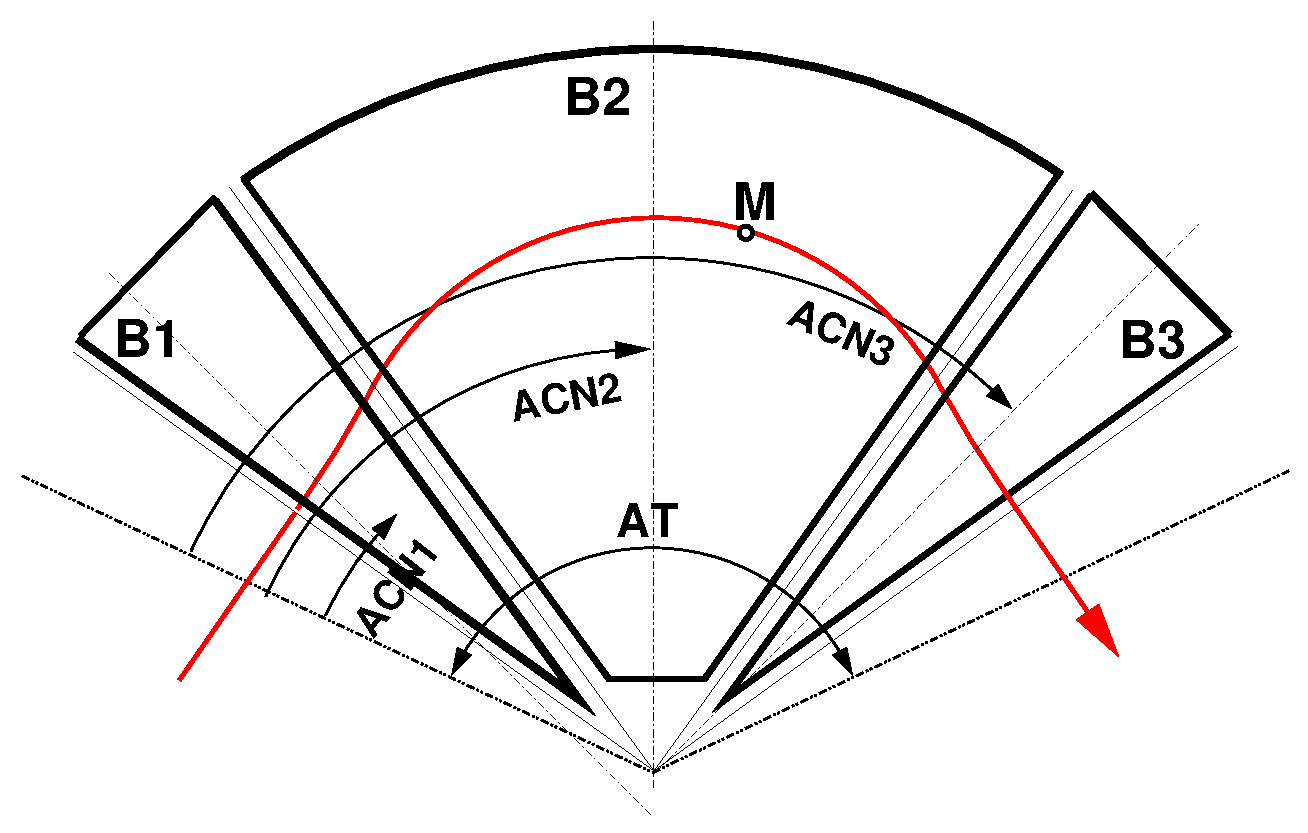
\includegraphics[width=8.5cm]{ffagTriplet.eps}  
 \caption{ \label{figFFAG}
Definition of a dipole $N$-tuple ($N=3$, a triplet here) using  the \textsl{DIPOLES} or  \textsl{FFAG}  procedures. 
}
  \end{center}
\end{figure}


\paragraph{Calculation of the field from a single dipole} 

 \noindent The magnetic field is calculated in  polar
coordinates.  At all $(R,\theta)$ in the median plane ($z=0$), the 
magnetic field  due  a single one (index $i$) of the  dipoles  of a $N$-tuple FFAG  magnet is written 

$$ \Bz_i(R,\theta) =  \Bz_{0,i} \, \mathcal{F}_i(R,\theta) \, \left(   R/R_M \right)^{K_i}  $$

\noindent wherein $\Bz_{0,i}$  is a reference field, at reference radius  $RM_{i}$, 
 whereas $ \mathcal{F}(R,\theta)$ is calculated as described below. 



\paragraph{Calculation of $\mathcal{F}_i(R,\theta) $} 

\noindent The fringe field coefficient  $\mathcal{F}_i(R,\theta) $ associated with a  dipole is computed as in the 
procedure  \textsl{DIPOLES} (eq.~\ref{EqFFdips}), including (rigorously if the interpolation method is 
used, to zero order if the analytic method is used)  radial dependence of the gap size 

\begin{equation}
\label{EqggvsR}
g(R) = g_0 \, (RM/R)^{\kappa}
\end{equation}

\noindent  so to simulate the effect of gap shaping of $ \Bz_i(R,\theta)$ on 
field fall-off,  over the 
all radial extent of a scaling FFAG dipole (with normally - but not in practice - $\kappa = K_i$). 
 

\bigskip

\paragraph{Calculation of the full field from all $N$ dipoles}

For the rest, namely, calculation of the full field at particle position from the $N$ dipoles, 
analytical   calculation or numerical interpolation of the  mid-plane field derivatives, 
extrapolation off median plane, etc., things are performed exactly as in the case of the 
 \textsl{DIPOLES} procedure (see page~\pageref{FFatAP}). 




\bigskip

\paragraph{Sharp edge} 

\noindent Sharp edge field fall-off at a field boundary  can only be simulated if the following conditions are fulfilled~: 

- entrance (resp. exit)  field boundary  coincides with entrance (resp. exit) 
dipole limit (it means in particular, see Fig.~\ref{fig9},  
$\omega^+= ACENT$ (resp. $\omega^- = -(AT-ACENT)$), 
together with $\theta=0$ at entrance (resp. exit) EFBs), 

- analytical method for calculation of the  mid-plane field derivatives is used. 







\newpage


\subsubsection*{FFAG-SPI~: \FFAGSPITitl} \label{FFAG-SPI} \index{FFAG magnet, spiral|textbf}
\medskip

\noindent \textsl{FFAG-SPI} works much like \textsl{FFAG} 
as to the field modelling, apart from the axial  dependence of the field. 

\bigskip

\noindent The \textsl{FFAG} procedure allows overlapping of fringe fields of neighboring dipoles, 
thus simulating in some sort the field in a dipole $N$-tuple - as for instance in an FFAG doublet 
or triplet (Fig.~\ref{figFFAGSPI}). This is done in the way described below. 

\bigskip

\noindent  The dimensionning of the magnet is defined by

\bigskip

 \begin{tabular}{>{\sl}l!{~:}l}
	 AT &  total angular aperture \\
	 RM & mean radius used for the positioning of field boundaries\\
 \end{tabular}

\bigskip

\noindent For each one of the $N=1$ to (maximum) $5$ dipoles of the  $N$-tuple, 
the two  effective field boundaries (entrance and exit EFBs) from which  the dipole field  is drawn are
defined from geometric boundaries, the shape and position of which are determined by the 
following parameters 

\bigskip

\begin{tabular}{l!{~:}l}
	$ACN_i$  & arbitrary inner angle, used for EFB's positioning  \\
	$\omega$ &  azimuth of an EFB with respect to  \textsl{ACN}\\
	$\xi$ & spiral angle \\
\end{tabular}

\bigskip

\noindent with $ACN_i$ and $\omega$ as defined in Fig.~\ref{figFFAGSPI} 
(similar to what can be found in Figs.~\ref{figFFAG} and \ref{fig9}-A). 

\begin{figure}[h]
 \begin{center}
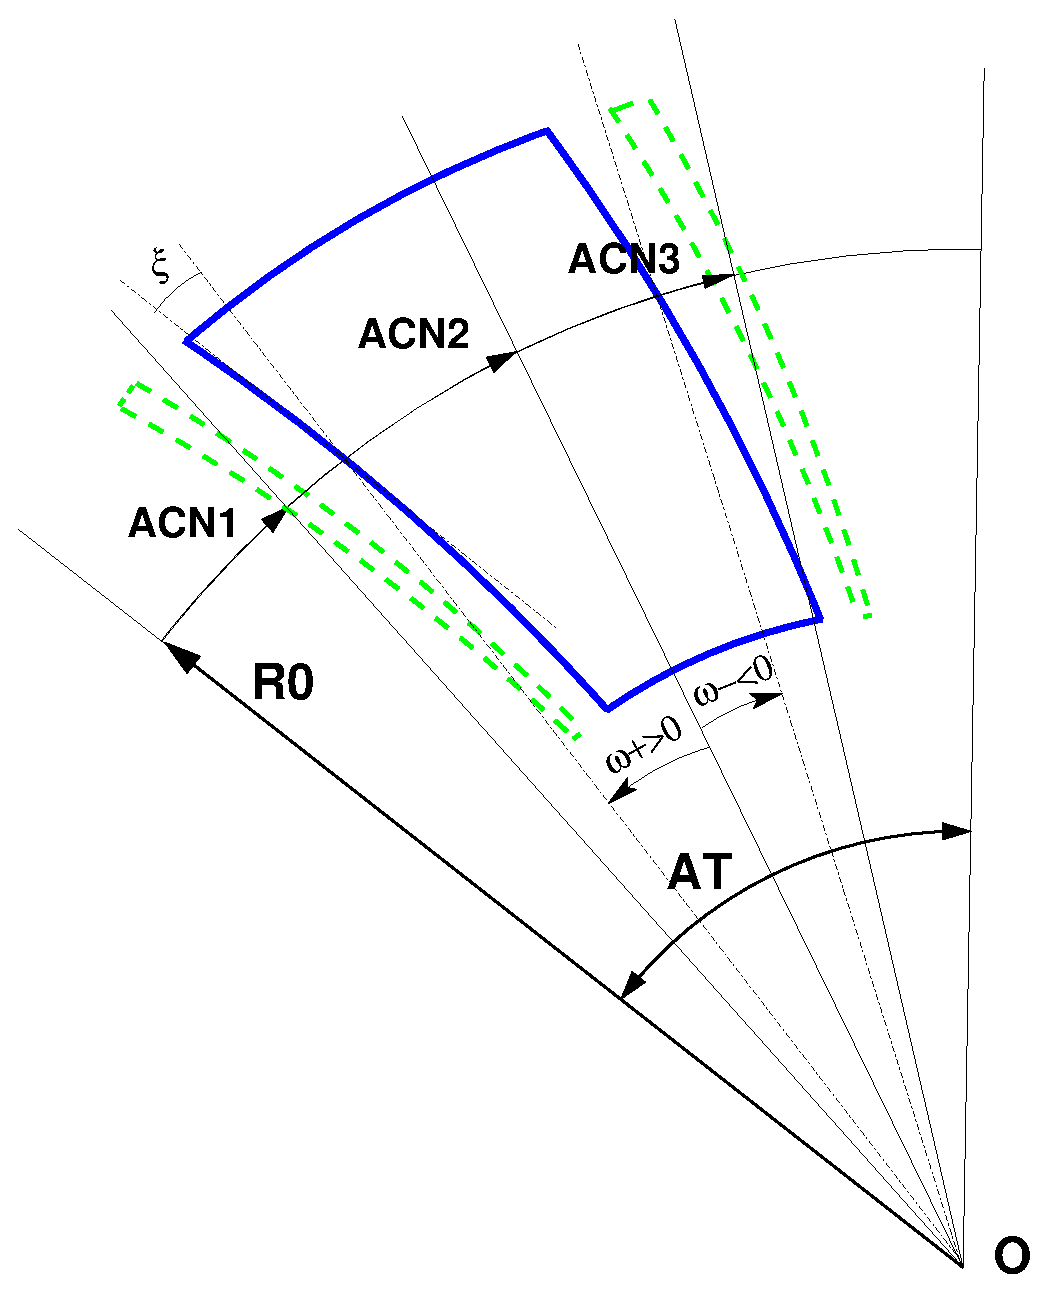
\includegraphics[width=7cm]{figFFAGSPI.eps}  
 \caption{ \label{figFFAGSPI}
A $N$-tuple spiral sector FFAG magnet ($N=3$ here, simulating active field clamps at 
entrance and exit side of a central dipole). 
}
  \end{center}
\end{figure}


\bigskip


\paragraph{Calculation of the field from a single dipole} 

 \noindent The magnetic field is calculated in  polar
coordinates.  At all $(R,\theta)$ in the median plane ($z=0$), the 
magnetic field  due  a single one (index $i$) of the  dipoles  of a $N$-tuple FFAG  magnet is written 

$$ \Bz_i(R,\theta) =  \Bz_{0,i} \, \mathcal{F}_i(R,\theta) \, \left(   R/R_M \right)^{K_i}  $$

\noindent wherein $\Bz_{0,i}$  is a reference field, at reference radius  $RM_{i}$, 
 whereas $ \mathcal{F}(R,\theta)$ is calculated as described below. 



\paragraph{Calculation of $\mathcal{F}_i(R,\theta) $} 

\noindent The fringe field coefficient  $\mathcal{F}_i(R,\theta) $ associated with a  dipole is computed as in the 
procedure  \textsl{DIPOLES} (eq.~\ref{EqFFdips}), including  radial dependence of the gap size 

\begin{equation}
%\label{EqggvsR}
g(R) = g_0 \, (RM/R)^{\kappa}
\end{equation}

\noindent  so to simulate the effect of gap shaping of $ \Bz_i(R,\theta)$ on 
field fall-off,  over the 
all radial extent of a scaling FFAG dipole (with normally - but not in practice - $\kappa = K_i$). 
 

\bigskip

\paragraph{Calculation of the full field from all $N$ dipoles}

For the rest, namely, calculation of the full field at particle position from the $N$ dipoles,  
analytical   calculation or numerical interpolation of the  mid-plane field derivatives, 
extrapolation off median plane, etc., things are performed exactly as in the case of the 
 \textsl{DIPOLES} procedure (see page~\pageref{FFatAP}). 





\newpage

\subsubsection*{MAP2D~: \MAPTwoDTitl~\cite{Pavel}} \label{MAP2D} \index{MAP2D|textbf}
\medskip

\textsl{MAP2D} reads a 2-D field map that provides the three
components $ B_X$, $ B_Y $, $ B_Z $ of the magnetic field at all nodes of a 2-D Cartesian 
uniform mesh in an $(X,Y)$ plane. 
No particular symmetry is assumed, which allows the 
treatment of any type of field (e.g., dipole field  with arbitrary $Z$ elevation 
- the map needs not be a mid-plane map, solenoidal field, etc.). The data file should be filed with a 
format that fits the following \FORTRAN reading sequence (presumably compatible 
with \textsl{TOSCA} code outputs) 

{\footnotesize
\begin{verbatim}
	      OPEN (UNIT = NL, FILE = FNAME, STATUS = `OLD' [,FORM='UNFORMATTED'])
	       DO 1 J=1,JY 
	          DO 1 I=1,IX
	             IF (BINARY) THEN
	                READ(NL) Y(J), Z(1), X(I), BY(I,J), BZ(I,J), BX(I,J)
	             ELSE
	                READ(NL,100) Y(J), Z(1), X(I), BY(I,J), BZ(I,J), BX(I,J)
	100             FORMAT (1X, 6E11.4)
	             ENDIF
      1        CONTINUE
\end{verbatim}}
\medskip

\noindent where $IX$ ($JY$) is the number of longitudinal (transverse horizontal) nodes of 
the 2-D uniform mesh, $Z(1) $ is the considered $Z$-elevation of the map. For 
binary files, FNAME must begin with \mbox{`B\_ '} or  \mbox{`b\_'}, a flag `BINARY' will thus be 
set to `.TRUE.'. The field $ \vec  B=(B_X,B_Y,B_Z )$ is next normalized with 
BNORM, prior to ray-tracing.  As well the  coordinates  X, Y are normalized with 
  \textsl{X-,Y-NORM} coefficients (usefull to convert to centimeters, the working units in  \zgoubi. 


\bigskip

\noindent At each step of the trajectory of a particle, the field and its 
derivatives are calculated by a polynomial interpolation followed 
by a $ Z $ extrapolation (see sections~\ref{sec2.3.3}, \ref{sec2.4.3}). Entrance and/or 
exit integration boundaries may be defined, in the same way as for \textsl{CARTEMES\index{CARTEMES}}.


\newpage

\subsubsection*{MAP2D-E~: \MAPTwoDETitl} \label{MAP2D-E} \index{MAP2D-E|textbf}
\medskip

\textsl{MAP2D-E} reads a 2-D field map that provides the three
components $ E_X$, $ E_Y $, $ E_Z $ of the electric field at all nodes of a 2-D Cartesian 
uniform mesh in an $(X,Y)$ plane. 
No particular symmetry is assumed, which allows the 
treatment of any type of field (e.g.,  field of a parallel-plate mirror with arbitrary $Z$ elevation 
- the map needs not be a mid-plane map). The data file should be filed with a 
format that fits the following \FORTRAN reading sequence 

{\footnotesize
\begin{verbatim}
	      OPEN (UNIT = NL, FILE = FNAME, STATUS = `OLD' [,FORM='UNFORMATTED'])
	       DO 1 J=1,JY 
	          DO 1 I=1,IX
	             IF (BINARY) THEN
	                READ(NL) Y(J), Z(1), X(I), EY(I,J), EZ(I,J), EX(I,J)
	             ELSE
	                READ(NL,100) Y(J), Z(1), X(I), EY(I,J), EZ(I,J), EX(I,J)
	100             FORMAT (1X, 6E11.4)
	             ENDIF
      1        CONTINUE
\end{verbatim}}
\medskip

\noindent where $IX$ ($JY$) is the number of longitudinal (transverse horizontal) nodes of 
the 2-D uniform mesh, $Z(1) $ is the considered $Z$-elevation of the map.   For 
binary files, FNAME must begin with \mbox{`E\_ '} or  \mbox{`b\_'}, a flag  `BINARY' will thus be 
set to `.TRUE.'. The field $ \vec  E=(E_X,E_Y,E_Z )$ is next normalized with 
ENORM, prior to ray-tracing.  As well the coordinates  X, Y re normalized with 
  \textsl{X-,Y-NORM} coefficients (usefull to convert to centimeters, the working units in  \zgoubi. 


\bigskip

\noindent At each step of the trajectory of a particle, the field and its 
derivatives are calculated by a polynomial interpolation followed 
by a $ Z $ extrapolation (see sections~\ref{sec2.3.3},~\ref{sec2.4.3}). Entrance and/or 
exit integration boundaries may be defined, in the same way as for \textsl{CARTEMES\index{CARTEMES}}.



\newpage

\subsubsection*{MARKER~: \MARKERTitl} \label{MARKER} \index{MARKER|textbf}
\medskip

\textsl{MARKER} does nothing. Just a marker. No data. 

As any other keyword, \textsl{MARKER} is allowed two \LABEL s. Using 
 '.plt' as a second \LABEL\ will cause storage of current coordinates into 
zgoubi.plt\index{LABEL@{\LABEL}}\index{zgoubi.plt} 



\newpage

\subsubsection*{MATPROD~:  \MATPRODTitl}\label{MATPROD}\index{MATPROD|textbf}
\medskip

\textsl{MATPROD} performs a matrix transfer of the particle coordinates 
in the following way 

$$ X_i = \sum_j R_{ij}X^0_j + \sum_{j,k} T_{ijk}X^0_jX^0_k $$
%
 where, $ X_i $ stands for any of the current coordinates $ Y$, $T$, $Z$, $P $, path length and dispersion, and $ X^0_i $ stands for any of the initial coordinates.
$[R_{ij}]$ ($[T_{ijk}]$) is the first order (second order) 
transfer matrix as usually involved in second order beam optics~\cite{Biblio10}.      %%% [10]  
Second order transfer is optional.  The length of the element represented by 
the matrix may be introduced for the purpose of path length updating.  
\medskip
Note~: \textsl{MATRIX\index{MATRIX}} delivers $[R_{ij}]$ and $[T_{ijk}]$ matrices in a format 
suitable for straightforward use with \textsl{MATPROD}.

\newpage

\subsubsection*{MULTIPOL~:  \MULTIPOLTitl} \label{MULTIPOL}\index{MULTIPOL}

The simulation of  multipolar magnetic field $ \vec  M $ by \textsl{MULTIPOL}  proceeds 
by addition of the dipolar  ($\vec  B1$),  quadrupolar ($ \vec  B2 $), sextupolar 
($ \vec  B3 $), etc., up to 20-polar  ($\vec  B10$) 
components, and of their derivatives up to fourth order, following

\begin{align*}
	\vec  M &   =   \vec B1+\vec  B2+\vec  B3+ \ ...\ +\vec  B10  \\ 
	\dfrac{ \partial\vec M }{ \partial X} 
	        &   = \dfrac{ \partial\vec  B1}{ \partial X} + 
	        \dfrac{\partial\vec  B2 }{ \partial X} + 
	        \dfrac{\partial\vec  B3}{ \partial X} + 
                            \ ...\ +
	        \dfrac{\partial\vec  B10 }{ \partial X} \\
	\dfrac{ \partial^ 2\vec  M }{ \partial X\partial Z} 
	       & = \dfrac{ \partial^ 2\vec  B1 }{ \partial X\partial Z} + 
	       \dfrac{\partial^ 2\vec  B2 }{ \partial X\partial Z} + 
	       \dfrac{\partial^ 2\vec  B3}{ \partial X\partial Z} + 
                            \ ...\ +
 	       \dfrac{\partial^ 2\vec  B10}{ \partial X\partial Z} \\
	\text{etc. } &
\end{align*}


\noindent The independent components $ \vec  B1$, $\vec  B2$, $\vec  B3$, ..., 
$ \vec  B10 $  and their derivatives up to the fourth order are calculated as described in 
 section~\ref{sec2.3.5}.  

\bigskip

\noindent The entrance and exit fringe fields are treated separately.  They
are characterized by the integration zone $ X_E $ at entrance and $ X_S $ at exit,
as for \textsl{QUADRUPO\index{QUADRUPO}}, and by the extent $ \lambda_ E $ at entrance, 
$\lambda_ S $ at exit. The fringe field extents for the dipole component are $ \lambda_ E $ 
and $ \lambda_ S $. The fringe field for the quadrupolar 
(sextupolar,  ..., 20-polar) component is given by a coefficient $ E_2 $ 
 ($E_3$, ..., $E_{10}$)  at entrance, and 
$ S_2 $ ($ S_3$, ..., $S_{10}$)  at exit, such that the extent is $ \lambda_ E\ast E_2$
 ($\lambda_ E\ast E_3$, ..., $\lambda_ E\ast E_{10}$)  at 
entrance and $ \lambda_ S\ast S_2 $  ($\lambda_ S\ast S_3$, ..., $\lambda_ S\ast S_{10}$)  
at exit. 
\bigskip

\noindent If $ \lambda_ E=0 $  ($\lambda_ S=0$)  the multipole lens is
considered to have a sharp edge field at entrance (exit), and then, $ X_E \ (X_S) $ is forced to zero 
(for the mere purpose of saving computing time).  If $ E_i=0 $  ($S_i=0$) ($i=2,\, 10$), the entrance (exit) fringe field for 
 the multipole component $ i $ is considered as a sharp edge field.  
In sharp edge field model, the wedge angle vertical first order focusing effect (if $\vec  B1$ is non zero) is simulated at magnet entrance and exit  by a kick $P_2 = P_1 - Z_1 \tan (\epsilon / \rho)$ applied to each particle ($P_1$, $P_2$ are the vertical angles upstream and downstream the EFB, $Z_1$ the vertical particle position at the EFB, $\rho$ the local horizontal bending radius and $\epsilon$ the wedge angle experienced by the particle~; $\epsilon$ depends on the horizontal angle T). 

\bigskip

\noindent Overlapping of fringe fields inside the optical element  is treated separately
for each component, in the way described in \textsl{QUADRUPO\index{QUADRUPO}}.  
\bigskip

\noindent Any multipole component $ \vec  Bi $ can be rotated independently
by an angle $ RXi $ around the longitudinal $ X$-axis, for the simulation of positioning defects,
as well as skewed lenses. 

\bigskip

\noindent Magnet (mis-)alignement is assured by \textsl{KPOS}. 
\textsl{KPOS} also  allows some degrees of automatic alignement useful for periodic structures (section~\ref{sec4.6.2}).



\newpage

\subsubsection*{OCTUPOLE~: \OCTUPOLETitl\  (Fig.~\protect\ref{fig24}) } \label{OCTUPOLE}

 The meaning of parameters for \textsl{OCTUPOLE} \index{OCTUPOLE} is the same as for 
\textsl{QUADRUPO\index{QUADRUPO}}.  In fringe field regions the magnetic field $ \vec  B(X,Y,Z)$ and 
its derivatives up to fourth order are derived from the scalar potential 
approximated to the 8-th order in $ Y $ and $ Z $

\begin{align*}
	V(X,Y,Z) &   =   \left(G-\dfrac{G^{\prime\prime} }{ 20} \, (Y^2+Z^2)+
	              \dfrac{G^{\quaprime} }{ 960}\, (Y^2+Z^2)^2 \right) (Y^3Z-YZ^3)   \\
	\text{with } G_0 &   =  \dfrac{ B_0 }{ R^3_0} 
\end{align*}

\noindent Outside fringe field regions, or everywhere in sharp edge dodecapole
($ \lambda_ E=\lambda_ S=0$) , $ \vec  B(X,Y,Z) $ in the magnet is given by 

\begin{align*}
	B_X &   =   0 \\
	B_Y &   =   G_0(3Y^2Z-Z^3)  \\
	B_Z &   = G_0(Y^3-3YZ^2)    
\end{align*}
\vfill

%%%%%%%%%%%%%%figure%%%%%%%%%%%%%%
\begin{figure}[H]
%\vspace{12 truecm}
%%%Figure 24
\centerline{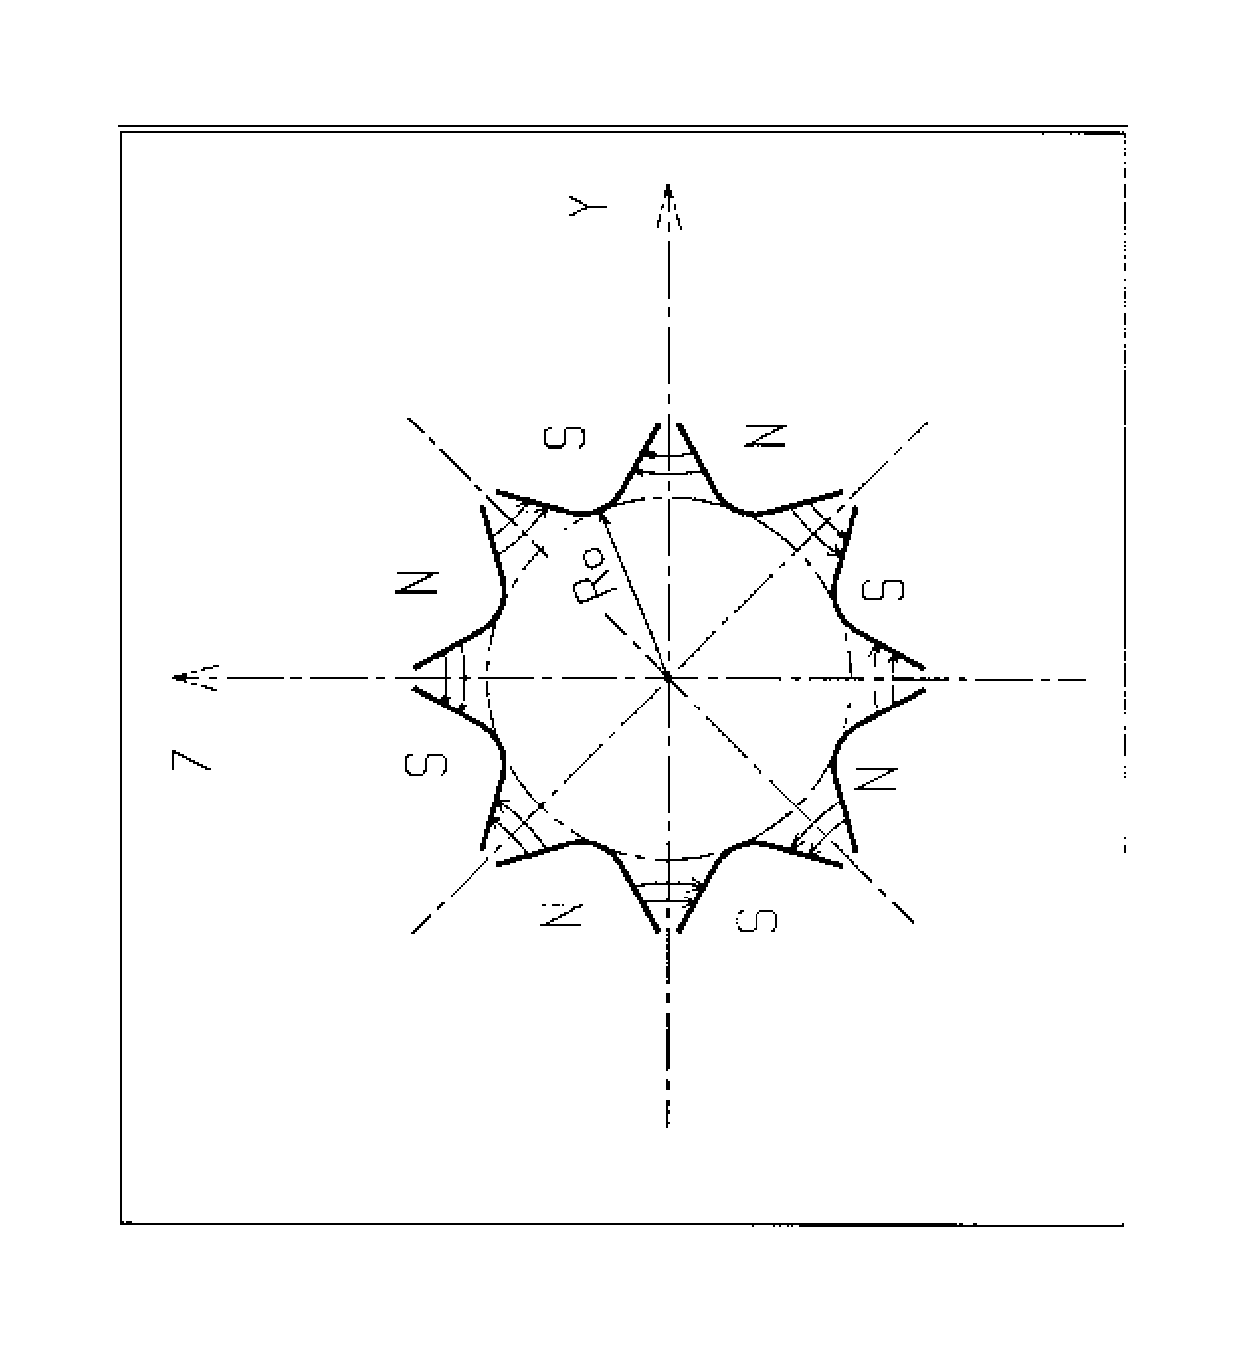
\includegraphics[height=12cm,angle=-90]{Fig24.ps}}
\caption{\label{fig24}Octupole magnet}
\end{figure}
\vfill

\newpage

\subsubsection*{POISSON~:\POISSONTitl} \label{POISSON} \index{POISSON}

This keyword allows reading a field profile $ B(X) $ from  \textsl{POISSON} output. 
Let \textsl{FNAME} be the name of this output file (normally,
\textsl{FNAME} = outpoi.lis\index{outpoi.lis})~; 
the data are read following the \FORTRAN statements hereunder 

{\footnotesize
\begin{verbatim}
	 I = 0
   11    CONTINUE
	   I = I + 1
           READ(LUN,101,ERR=10,END=10) K, K, K, R, X(I), R, R, B(I) 
   101     FORMAT(I1, I3, I4, E15.6, 2F11.5, 2F12.3)
         GOTO 11     
   10    CONTINUE
         ...
\end{verbatim}}
\medskip
 
\noindent where X(I) is the longitudinal coordinate, and B(I) is the Z
component of the field at a node (I) of the mesh. K's and R's are dummy variables 
appearing in the \textsl{POISSON} output file outpoi.lis
 but not used here. 
\bigskip

\noindent From this field profile, a 2-D median plane map is built up, with a 
rectangular and uniform mesh~; mid-plane symmetry is assumed. The field at 
each node $ (X_i,Y_j) $ of the map is $ B(X_i) $, independent of $ Y_j $
(\emph{i.e.}, the distribution is uniform in the $ Y $ direction).  
\bigskip

\noindent For the rest, \textsl{POISSON} works in a way similar to \textsl{CARTEMES\index{CARTEMES}}. 

\newpage
\subsubsection*{POLARMES~: \POLARMESTitl} \label{POLARMES} \index{POLARMES}

Similar to \textsl{CARTEMES\index{CARTEMES}}, apart from the polar 
mesh frame~: $IX$ is the number of angular nodes, $JY$ the number of 
radial nodes~; $X(I)$ and $Y(J)$ are respectively the angle and radius 
of a node (these parameters are similar to those entering in the 
definition of the map in \textsl{DIPOLE-M}\index{DIPOLE-M}).

\newpage

\subsubsection*{PS170~: \PSusoTitl} \label{PS170} \index{PS170}

\textsl{PS170} is dedicated to a `rough' simulation
of CERN's \textsl{PS170} dipole.  
\bigskip

\noindent The field $ B_0 $ is constant inside the magnet, and zero outside. 
The pole is a circle  of radius $ R_0 $, centered on $ X $ axis.  The output coordinates are
generated at the distance \textsl{\XL} from the entrance (Fig.~25).  %%%
\vfill

%%%%%%%%%%%%%%figure%%%%%%%%%%%%%%
\begin{figure}[H]
%\vspace{17 truecm}
%%%Figure 25
\centerline{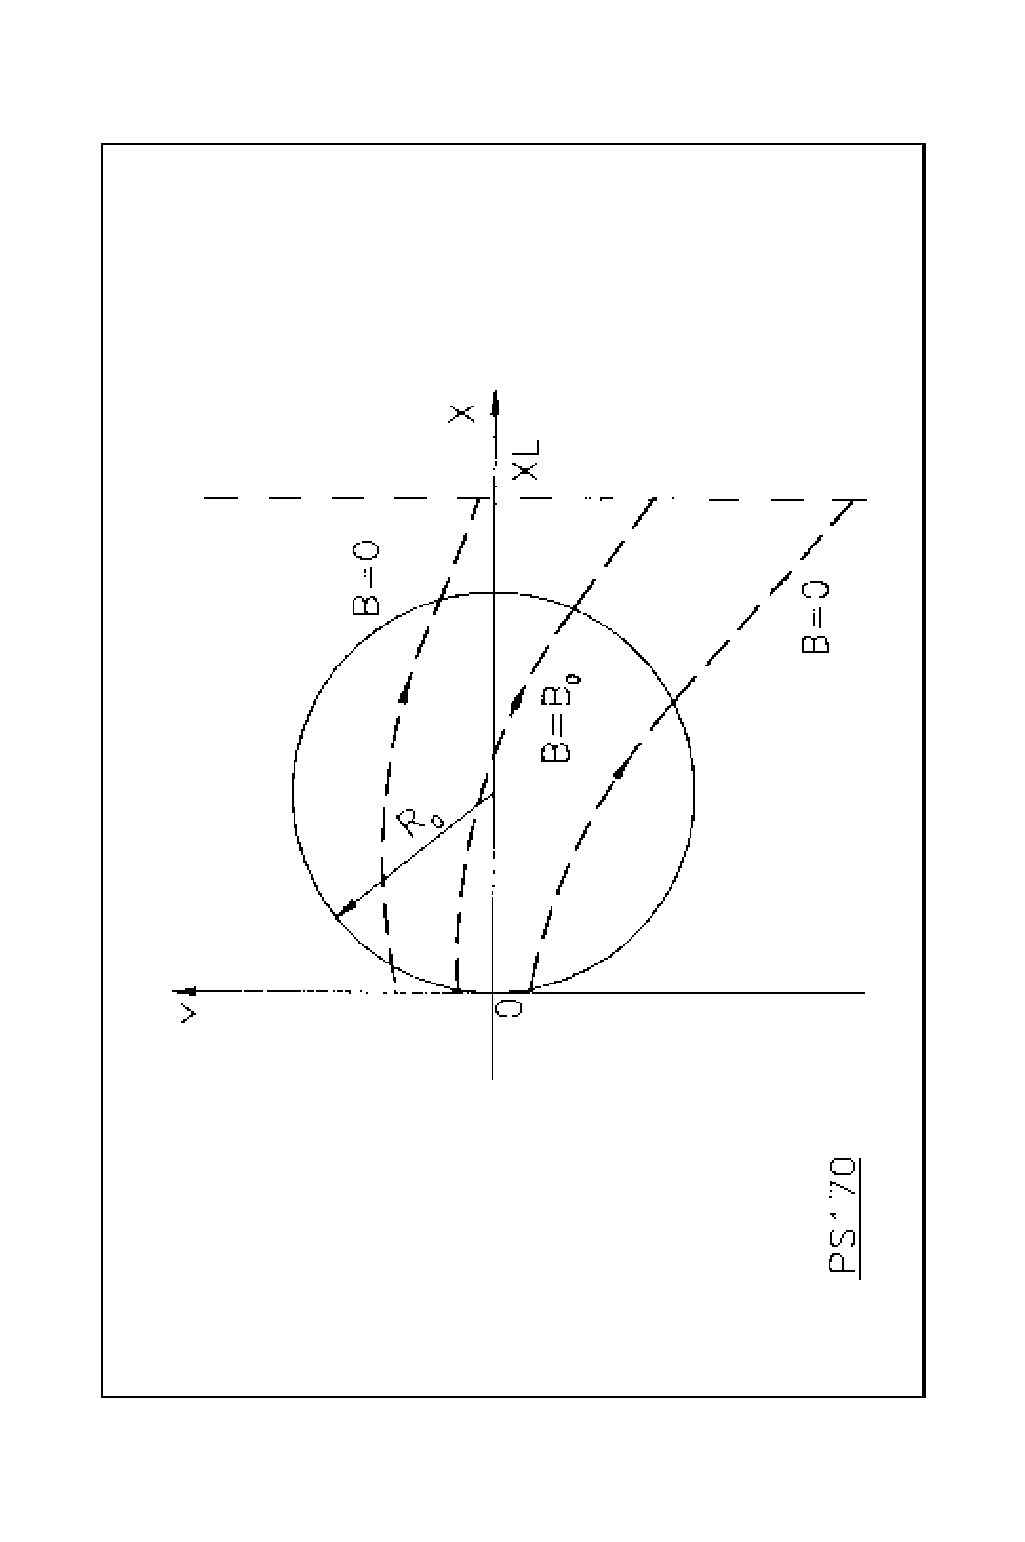
\includegraphics[height=15cm,angle=-90]{Fig25.ps}}
\caption{\label{fig25}Scheme of the PS170 magnet simulation.}
\end{figure}
\vfill

\newpage

\subsubsection*{QUADISEX, SEXQUAD~: \QUADISEXTitl} \label{QUADISEX}\label{SEXQUAD}
\index{QUADISEX} \index{SEXQUAD}

\textsl{SEXQUAD}    defines in a simple way a sharp edge field with quadrupolar, 
sextupolar and octupolar components. \textsl{QUADISEX}  adds a dipole component. The length of 
the element is $ \XL $.  The vertical component $ B \equiv B_Z(X,Y,Z=0) $ of the field and its derivatives in median plane are 
calculated at each step from the following expressions 

\begin{align*}
	B &   =     B_0
	           \left(U+ \dfrac{N }{ R_0}Y + 
	                \dfrac{B }{ R^2_0} Y^2+ \dfrac{G }{ R^3_0} Y^3 \right)  \\
	\dfrac{ \partial B }{ \partial Y} 
	   &   =   B_0 \left(
	             \dfrac{N }{ R_0} + 2 \dfrac{B }{ R^2_0} Y + 3\dfrac{G }{ R^3_0}Y^2 \right) \\  
	\dfrac{ \partial^ 2B }{ \partial Y^2} 
	  &  =     B_0 \left(2 \dfrac{B }{ R^2_0} + 6\dfrac{G }{ R^3_0} Y \right) \\
	\dfrac{ \partial^ 3B }{ \partial Y^3}  
	   & =     6B_0 \,  \dfrac{G }{ R^3_0}
\end{align*}  
   %
    and then extrapolated out of the median plane by Taylor expansion in $ Z $ 
(see section~\ref{sec2.3.2}).
\bigskip

\noindent With option \textsl{SEXQUAD}, $ U=0$,  while with \textsl{QUADISEX}, $U=1 $. 

\newpage

\subsubsection*{QUADRUPO~:  \QUADRUPOTitl\  (Fig.~\protect\ref{fig26}) } \label{QUADRUPO}  
\index{QUADRUPO}

The length of the magnet $ \XL $ is the distance between the
effective field boundaries (EFB). The field at the pole tip $ R_0 $ is $ B_0 $. 

\noindent The extent of the  entrance (exit) fringe field is characterized by 
$ \lambda_ E(\lambda_ S) $.  The distance of ray-tracing on both sides of the
EFB's, in the field fall off regions, will be $\pm$  $ X_E $ at 
the entrance, and $\pm$  $ X_S $ at the exit (Fig.~\ref{fig27}),  
by prior and further automatic 
changes of frame. 

\noindent In the fringe field  regions $[ -X_E,X_E ]$  and 
$[ -X_S,X_S ]$ on both sides of the EFB's, $ \vec  B(X,Y,Z) $ and its derivatives up to
fourth order are calculated at each step of the trajectory from the analytical expressions 
of the three components $ B_X $, $ B_Y $, $ B_Z $ obtained by differentiation
of the scalar potential (see section~\ref{sec2.3.5}) approximated to the 8th order in $ Y $ 
and $ Z $. 

 \begin{gather*}
 	V(X,Y,Z)     =   \left(G- \dfrac{G^{\prime\prime} }{ 12}\, (Y^2+Z^2)+
	             \dfrac{G^{\quaprime} }{ 384}\, (Y^2+Z^2)^2-
	             \dfrac{G^{\cinqprime\prime} }{ 23040}\, (Y^2+Z^2)^3 \right)YZ  \\
	(G^\prime     =    dG/dX,\quad G^{\prime\prime} =d^2G/dX^2,...) \\
\intertext{where $ G $ is the gradient on axis~\protect\cite{Biblio12}~:  } %% [12]
    G(s) = \dfrac{G_0 }{ 1+ \exp  P(s)}\qquad \text{with} \quad G_0=\dfrac{B_0}{R_0} \\
\intertext{and,}
     P(s) = C_0
       +C_1 \left(  \dfrac{s }{ \lambda} \right) 
       +C_2 \left( \dfrac{s }{ \lambda} \right)^2 
       + C_3 \left( \dfrac{s }{ \lambda} \right)^3 
       +C_4 \left( \dfrac{s }{ \lambda} \right)^4 
       + C_5 \left(\dfrac{s }{ \lambda} \right)^5
       P(s)=C_0+C_1 \left(\dfrac{s }{ \lambda} \right) + C_2 \left(\dfrac{s }{ \lambda}\right)
\end{gather*}
%
 where, $ s $ is the distance to the field boundary and $\lambda$
stands for $ \lambda_ E $ or $ \lambda_ S $ 
(normally, $ \lambda  \simeq  2  \ast  R_0$). 

\noindent When fringe fields overlap inside the magnet $ (\XL\leq X_E+X_S)$,  
the gradient $ G $ is expressed as 

$$ G = G_E+G_S-1 $$
%
where, $ G_E $ is the entrance gradient and $ G_S $ is the exit gradient. 

\noindent If $ \lambda_ E=0$ ($\lambda_ S=0$),  the field at entrance 
(exit) is considered as sharp edged, and then $ X_E(X_S) $ is forced to zero 
(for the mere purpose of saving computing time). 

\noindent Outside of the fringe field regions (or everywhere when 
$ \lambda_E=\lambda_ S=0$)   $ \vec  B(X,Y,Z) $ in the magnet is given by 

\begin{align*}
	B_X &   =     0 \\
	B_Y &   =    G_0Z \\
	B_Z &   =     G_0Y  
\end{align*}

\newpage

%%%%%%%%%%%%%%figure%%%%%%%%%%%%%%
\begin{figure}[H]
%\vspace{9 truecm}
%%%Figure 26
\centerline{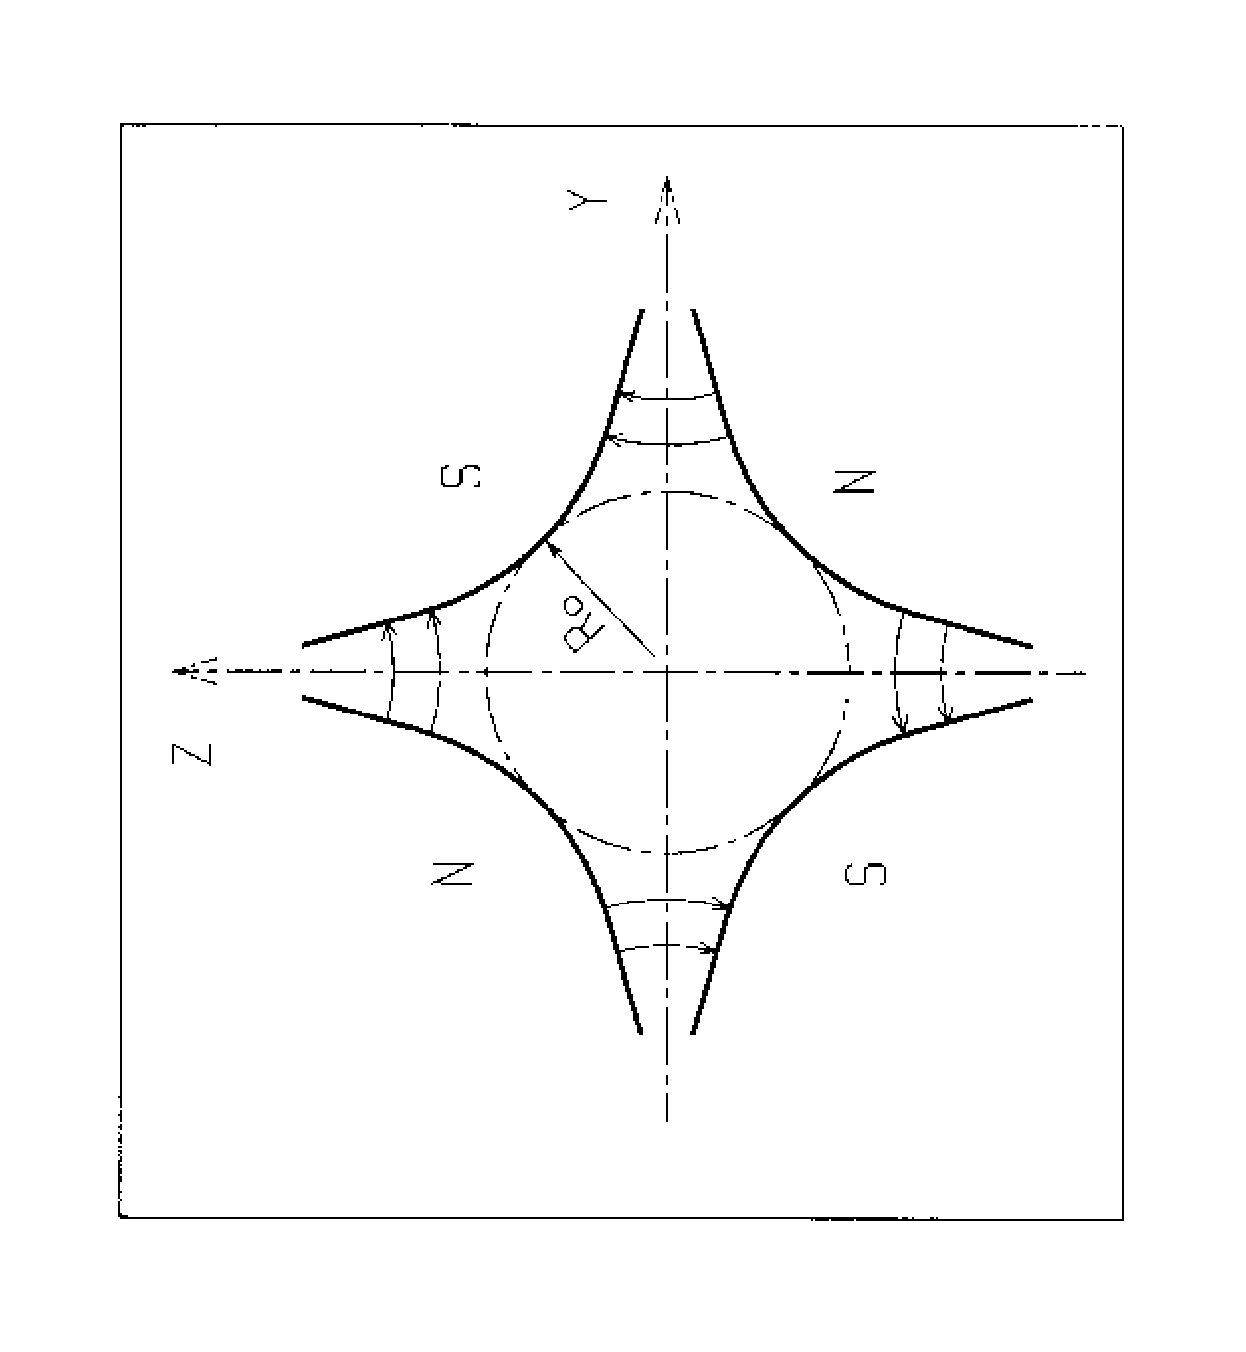
\includegraphics[height=10cm,angle=-90]{Fig26.ps}}
\caption{\label{fig26}Quadrupole magnet}
\end{figure}
\vfill
%%%%%%%%%%%%%%figure%%%%%%%%%%%%%%
\begin{figure}[H]
%\vspace{11 truecm}
%%%Figure 27
\centerline{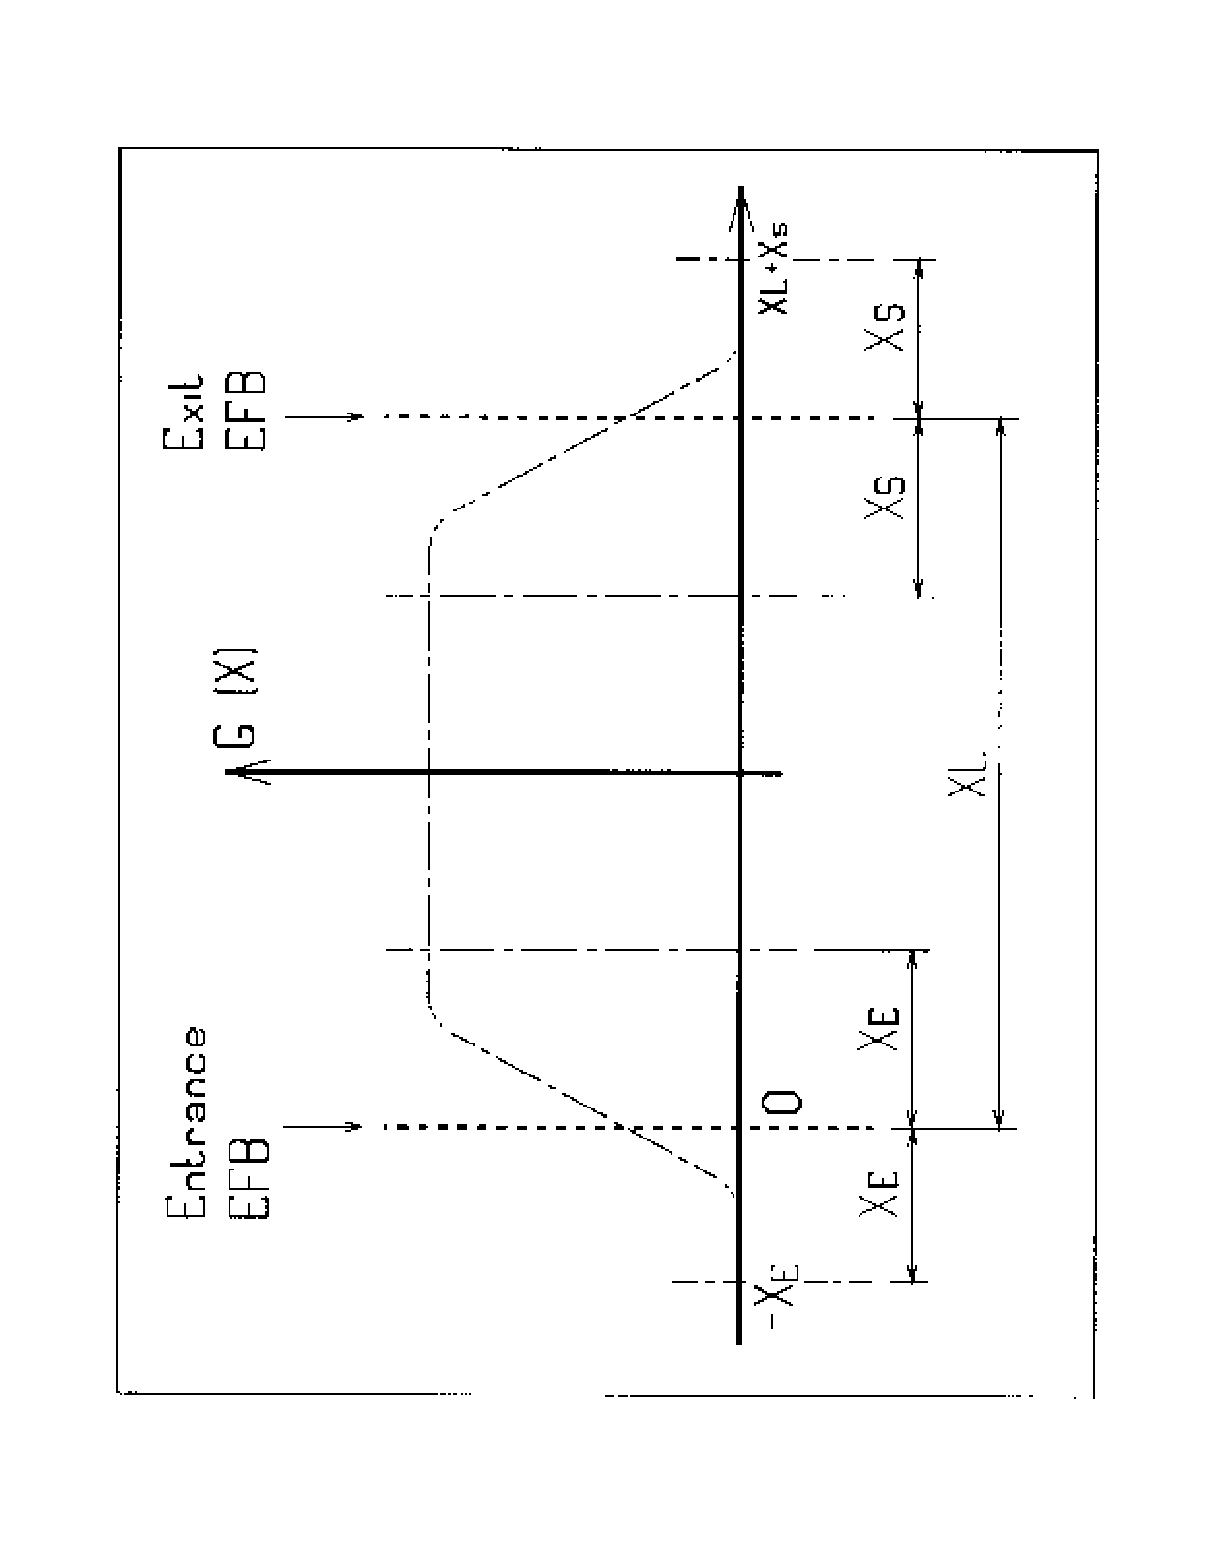
\includegraphics[height=10cm,angle=-90]{Fig27.ps}}
\hangcaption[Fig27]{\label{fig27}Scheme of the longitudinal field gradient $ G(X) $.\\
$ (OX) $ is the longitudinal axis of the reference frame $ (0,X,Y,Z) $ of \zgou.
The length of the element is $ \XL $, but trajectories 
are ray-traced from $ -X_E $ to $ \XL+X_S $, by means of prior and further
automatic changes of frame.}
\end{figure}

\newpage

\subsubsection*{SEPARA~: \SEPARATitl}\label{SEPARA} \index{SEPARA}

\textsl{SEPARA}  provides an analytic simulation of an electrostatic separator. 
Input data are the length $ L $ of the element, the electric field $ E $ and
the magnetic field $ B $. The mass $ m $ and charge $ q $ of the particles are
entered by means of the keyword \textsl{PARTICUL\index{PARTICUL}}.  
\medskip

\noindent The subroutines involved in this simulation solve the following
system of three equations with three unknown variables $ S$, $Y$, $Z $ (while  $ X\equiv L $), that 
describe the cycloidal motion of a particle in $ \vec  E$,  $ \vec  B $ static
fields (Fig.~\ref{fig28}).   

\begin{align*}
	X &   =   -R  \cos \left( \dfrac{\omega S }{ \beta c} + \epsilon \right) 
	         -  \dfrac{\alpha S }{ \omega\beta c} + \dfrac{C_1 }{ \omega} \\
	Y &   =     R \sin  \left(\dfrac{\omega S }{ \beta c} + \epsilon \right) - 
	         \dfrac{\alpha }{ \omega^ 2} - \dfrac{C_2 }{ \omega}  + Y_0  \\
	Z &   =  S \sin (P_0)+Z_0   
\end{align*}
%
 where, $ S $ is the path length in the separator, $\alpha =-\dfrac{Ec^2 }{ \gamma}$ ,
   $   \omega =-\dfrac{Bc^2 }{m\gamma}$, $   C_1=\beta \sin (T_0) \cos (P_0) $ 
and $ C_2=\beta c  \cos (T_0) $ $ \cos (P_0) $ are initial conditions. 
$c$ = velocity of light, $ \beta c$ = velocity of the particle,  
$ \gamma =(1-\beta^ 2)^{-\frac{1 }{ 2}} $ 
and  $\tan \epsilon  =   (C_2+ \frac{\alpha}{\omega})/C_1 $.   $ Y_0$,   $ T_0$,  
$Z_0$,  $ P_0 $ are the initial 
coordinates of the particle in the \zgou\ reference  frame.  Here 
$\beta c $ and $\gamma$ are assumed constant, which is true as long as the change of momentum
due to the electric field remains negligible all along the separator.  
\medskip

\noindent The index $IA$ in the input data allows switching to inactive
element (thus equivalent to \textsl{ESL}), horizontal or vertical separator.  
Normally, $ E$,  $B $ and the value of $ \beta_W $ for wanted particles are related by 

$$ B(T) = - \dfrac{E\left(\dfrac{V }{ m}\right) }{ \beta_ W\cdot c\left(\dfrac{m }{ s}\right)} $$

 %\newpage
\vfill

%%%%%%%%%%%%%%figure%%%%%%%%%%%%%%
\begin{figure}[H]
%\vspace{20 truecm}
%%%Figure 28
\centerline{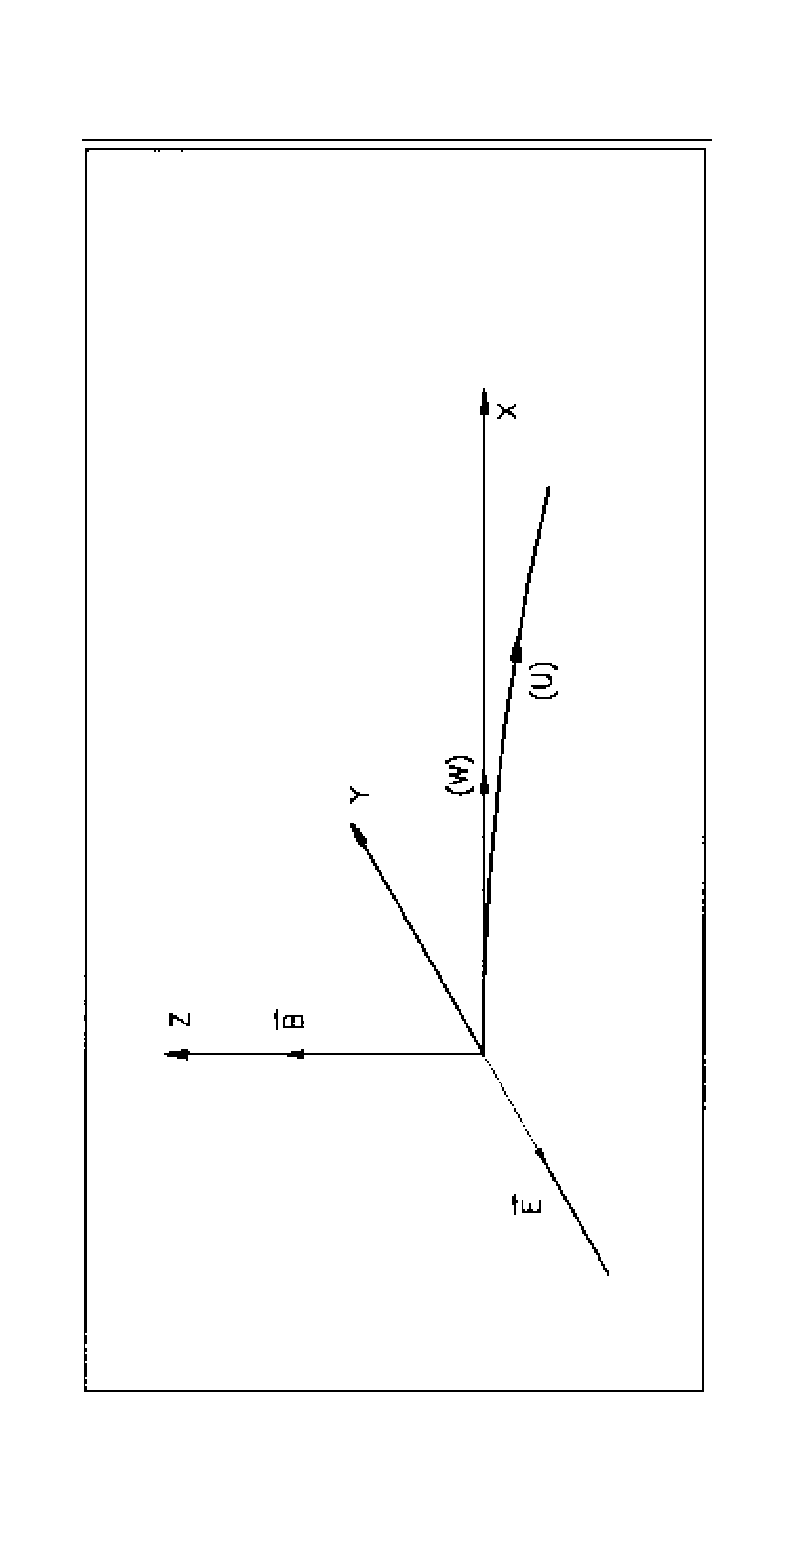
\includegraphics[height=15cm,angle=-90]{Fig28.ps}}
{\setlength{\captionwidth}{14cm}
\hangcaption[Fig28]{\label{fig28}Horizontal separation between a wanted particle, $ (W)$,  
and an unwanted particle, $ (U) $.  
$ (W) $ undergoes a linear motion while $ (U) $ undergoes a 
cycloidal motion.} }
\end{figure}
\vfill

\newpage

\subsubsection*{SEXTUPOL~: \SEXTUPOLTitl\ (Fig.~\protect\ref{fig29})} 
     \label{SEXTUPOL} \index{SEXTUPOL}  

The meaning of parameters for \textsl{SEXTUPOL} is the same as 
for \textsl{QUADRUPO\index{QUADRUPO}}.  
\medskip

\noindent In fringe field regions the magnetic field $ \vec  B(X,Y,Z) $ and
its derivatives up to fourth order are derived from the scalar potential approximated to 
7th order in $ Y $ and $ Z $

 \begin{align*}
 	V(X,Y,Z)    & =   \left(G- \dfrac{G^{\prime\prime} }{ 16}\, (Y^2+Z^2)+
	             \dfrac{G^{\quaprime} }{ 640}\, (Y^2+Z^2)^2\right) 
	             \left(Y^2Z-\dfrac{Z^3 }{ 3} \right)   \\
\text{with } G_0 &   =  \dfrac{ B_0}{ R^2_0}
\end{align*}

\noindent Outside fringe field regions, or everywhere in sharp edge sextupole 
($ \lambda_E=\lambda_ S=0$),   $ \vec  B(X,Y,Z) $ in the magnet is given by 

\begin{align*}
	B_X &   =     0 \\
	B_Y &   =    2G_0YZ \\
	B_Z &   =     G_0(Y^2-Z^2)  
\end{align*}
\vfill

%%%%%%%%%%%%%%figure%%%%%%%%%%%%%%
\begin{figure}[H]
%\vspace{12 truecm}
%%%Figure 29
\centerline{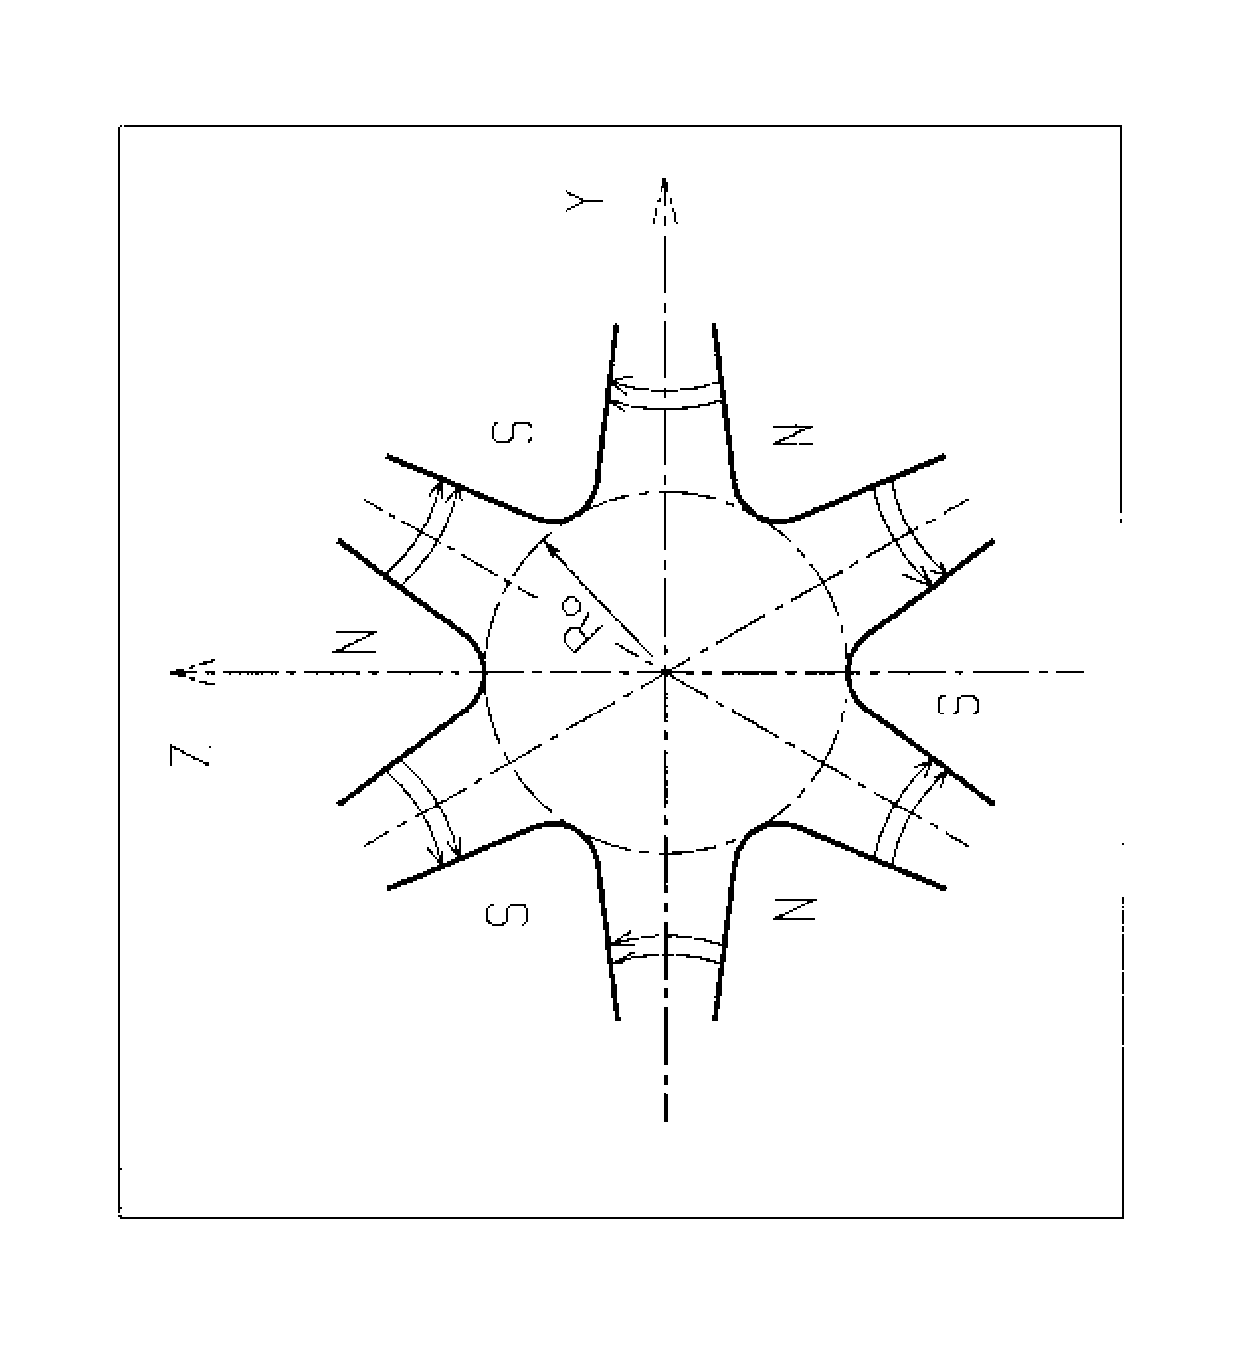
\includegraphics[height=12cm,angle=-90]{Fig29.ps}}
\caption{\label{fig29}Sextupole magnet}
\end{figure}
\vfill

\newpage

\subsubsection*{SOLENOID~: \SOLENOIDTitl\ (Fig.~\protect\ref{fig30}) } \label{SOLENOID} \index{SOLENOID} 

 The solenoidal magnet has an effective length $ \XL$,  a mean radius
$ R_0 $ and an asymptotic field  $ B_0=\mu_0 N I / \XL$ (i.e., $\int_{-\infty}^\infty 
B_X(X,r) dX = \mu_0 N I, ~\forall r<R_0$), wherein $B_X$=longitudinal field component, 
$ NI $  = number of Ampere-Turns, $\mu_0=4\pi  10^{-7} $. 
\medskip

\noindent The distance of ray-tracing beyond the effective length $ \XL$,   is 
$X_E $ at the entrance, and $ X_S $ at the exit (Fig.~\ref{fig30}).   
\medskip

\noindent The field $ \vec  B(X,r)$, $r=(Y^2+Z^2)^{1/2} $, and its derivatives
up to the second order with respect to $ X$, $Y $ or $ Z $ are obtained after 
the method proposed in ref.~\cite{Biblio17}, %%% [17]
that involves the three complete elliptic integrals $K$, $E $ and $\Pi$. These 
are calculated with the algorithm proposed in the same reference. Their 
derivatives are calculated by means of recursive relations~\cite{Biblio18}.  %%[18] 
\medskip

\noindent This analytical model for the solenoidal field allows simulating an 
extended range of coil geometries (legnth and radius) 
provided that the coil thickness is small enough compared to the mean radius $ R_0 $. 
\medskip


\noindent In particular the field on-axis writes (taking $x=r=0$ as solenoid center) 
$$B_X(x,r=0) = \frac{\mu_0 N I }{2 \XL} \left[ \frac{\XL/2-x}{\sqrt{(\XL/2-x)^2}+R_0^2} 
+  \frac{\XL/2+x}{\sqrt{(\XL/2+x)^2}+R_0^2} \right]$$ 
 and yields the magnetic length 
$$L_{mag} \equiv  \frac{\int_{-\infty}^\infty B_X(x,r<R_0) dx }{B_X(x=r=0)} 
= \XL\sqrt{1+\frac{4R_0^2 }{\XL^2}} > \XL $$ 
with in addition 
$$B_X(\textrm{center}) \equiv B_X(x=r=0) = 
      \frac{\mu_0 N I }{\XL\sqrt{1+\frac{4R_0^2}{\XL^2}}}.$$
\vfill

%%%%%%%%%%%%%%figure%%%%%%%%%%%%%%
\begin{figure}[H]
%\vspace{14 truecm}
%%%Figure 30
\centerline{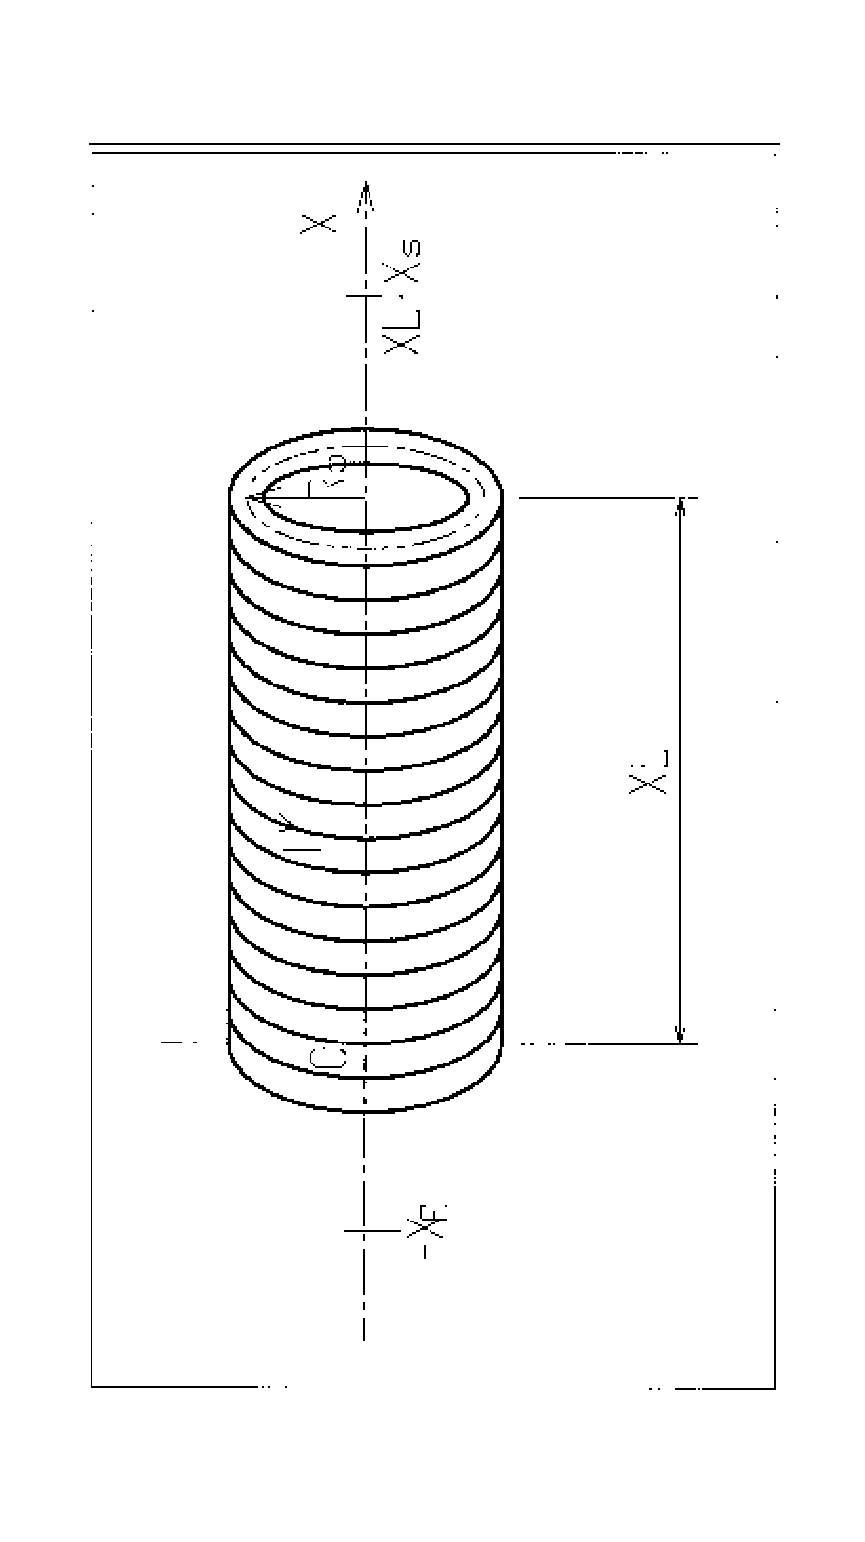
\includegraphics[height=15cm,angle=-90]{Fig30.ps}}
\caption{\label{fig30} Solenoidal magnet.}
\end{figure}
\vfill




\newpage

\subsubsection*{TOSCA~: \TOSCATitl} \label{TOSCA} \index{TOSCA}
\medskip

 \textsl{TOSCA} is dedicated to the reading and treatment of 2-D or 
3-D Cartesian or cylindrical mesh field maps as  delivered by the
\textsl{TOSCA}  magnet computer code standard output.
\bigskip

\noindent The total number of field data files to be read is given by the 
parameter $IZ$ that appears in the data list following the keyword. 
Each file contains the field components $B_X$, $B_Y$, $B_Z$ on an 
($X$, $Y$) mesh at a given $Z$ coordinate. $IZ = 1$ for 2-D~maps, and 
in this case $B_X$ and $B_Y$ are assumed  zero all over the map\footnote{Use 
\textsl{MAP2D}\index{MAP2D} in case non-zero $B_X$, $B_Y$ are to be taken into account in a 2-D map.}. 
For 3-D~maps with mid-plane symmetry, $IZ\ge 2$, and thus, the first 
data file whose name follows in the data list is supposed to contain the median 
plane field (assuming $ Z=0 $ and  $ B_X=B_Y=0$), while the next 
file(s) contain the next maps in increasing Z order. For arbitrary 3-D~maps 
(and in particular, contrary to what precedes without 
mid-plane symmetry assumption), following \textsl{MOD} value, see below, 
 the total number of maps (whose names follow in the data list) 
is $IZ$, and  map number $[IZ/2]+1$ is the $Z = 0$ one.
\bigskip

\noindent The field map data files should be formatted following the \FORTRAN reading 
sequence below.

{\footnotesize
\begin{verbatim}
	   DO  1  K = 1, KZ
	     OPEN (UNIT = NL, FILE = FNAME, STATUS = `OLD' [,FORM='UNFORMATTED'])
	     DO  1  J = 1,  JY  
	       DO  1 I = 1, IX
                 IF (BINARY) THEN
                   READ(NL) Y(J), Z(K), X(I), BY(J,K,I), BZ(J,K,I), BX(J,K,I)
                 ELSE
	           READ(NL,100) Y(J), Z(K), X(I), BY(J,K,I), BZ(J,K,I), BX(J,K,I)
    100	           FORMAT(1X,6E11.2)
                 ENDIF
     1     CONTINUE
\end{verbatim}}
\medskip

\noindent where, $IX$ ($JY$, $KZ$)  is   the number of longitudinal 
(transverse horizontal, vertical) nodes of the 3-D uniform mesh. For binary files, 
FNAME must begin with  \mbox{`B\_'} or  \mbox{`b\_'}, a flag  `BINARY' will thus be set to `.TRUE.'.  

A flag \textsl{MOD} determines wether Cartesian or Z-axis cylindrical mesh is used. \textsl{MOD} can 
take various values depending also on the map data file formatting. (To be documented - see FORTRAN 
subroutine FMAPW and its entries FMAPR, FMAPR2.)

\bigskip

\noindent The field $ \vec  B=(B_X,B_Y,B_Z) $ is normalized by means of 
\textsl{BNORM} in a similar way as in \textsl{CARTEMES\index{CARTEMES}}.  
 As well the  coordinates  X (and Y, Z with 3-D field maps) is normalized with 
a  \textsl{X-[Y-,Z-]NORM} coefficient (usefull to convert to centimeters, the working units in  \zgoubi. 


\bigskip

\noindent At each step of the trajectory of a particle inside the map, the
field and its derivatives are calculated 

 - in the case of 2-D map,  by means of a second or fourth order polynomial interpolation, 
depending on \textsl{IORDRE\index{IORDRE}} (\textsl{IORDRE} = 2, 25 or 4), as for 
\textsl{CARTEMES\index{CARTEMES}}, 

 - in the case of 3-D map, by means of a second order polynomial interpolation with a 
$3  \times   3   \times   3$-point parallelipipedic grid, as described in 
section~\ref{sec2.4.4}. 
\bigskip

\noindent Entrance and/or exit integration boundaries between which the trajectories
are integrated in the field may be defined, in the same way as in  \textsl{CARTEMES\index{CARTEMES}}. 





\newpage

\subsubsection*{TRAROT~: \TRAROTTitl} \label{TRAROT} \index{TRAROT}

UNDER DEVELOPEMENT. Check before use. 

~

This procedure transports particles into a new frame by translation and rotation. Effect on spin tracking\index{spin tracking}, 
particle decay and gas-scattering are taken into account (but not on synchrotron radiation).





\newpage


\subsubsection*{UNDULATOR~: \UNDULATORTitl}\label{UNDULATOR}  \index{UNDULATOR}

\textsl{UNDULATOR} 


\bigskip

\noindent {\it To be documented}

\vfill
%%%%%%%%%%%%%%%figure%%%%%%%%%%%%%%
\begin{figure}[H]
  \vspace{5cm}
  %%%Figure Undulator
%  \centerline{\includegraphics[height=12cm,angle=-90]{FigUndul.eps}}
  {\setlength{\captionwidth}{12cm}
	\hangcaption[FigUndul]{\label{figUndul}
               Undulator magnet. 
    } }
\end{figure}
\vfill

\newpage

\subsubsection*{UNIPOT~: \UNIPOTTitl} \label{UNIPOT} \index{UNIPOT}

The lens is cylindrically symmetric about the $ X$-axis.  
\bigskip

\noindent The length of the first (resp. second, third) electrode is $ X1 $
(resp. $ X2$, $X3$). The distance between the electrodes is $ D$.  
The potentials are $ V1 $ and $V2$.  The inner radius is $ R_0 $ (Fig.~\ref{fig31}).  
The model for the electrostatic potential along the axis is~\cite{Biblio19}  %% [19]

$$ V(x) = 
    \dfrac{V2-V1 }{ 2\omega D} \left[
    \ln\, \dfrac{\cosh 
    	\dfrac{\omega \left(x+ \frac{X2}{ 2}+D \right) }{ R_0} }{
       \cosh \dfrac{\omega \left(x+\frac{X2 }{ 2}\right) }{ R_0}}  
    + \ln\,  \dfrac{\cosh \dfrac{\omega \left(x-\frac{X2 }{ 2}-D\right) }{R_0} }{
       \cosh \dfrac{\omega \left(x-\frac{X2 }{ 2}\right) }{R_0} }
     \right] $$
%
($ x  = $ distance from the center of the central electrode~;
$\omega$  = 1,318~; cosh = hyperbolic cosine), from which the field $ \vec  E(X,Y,Z) $ and its
derivatives are deduced following the procedure described in section~\ref{sec2.5.2}. 

\noindent Use \textsl{PARTICUL\index{PARTICUL}} prior to \textsl{UNIPOT}, for the
 definition of particle mass and charge.

\bigskip

\noindent The total length of the lens is $X1+X2+X3+2\,D$~; stepwise integration starts 
at entrance of the first electrode and terminates at exit of the third one. 

\vfill

%%%%%%%%%%%%%%figure%%%%%%%%%%%%%%
\begin{figure}[H]
%\vspace{14 truecm}
%%%Figure 31
\centerline{\includegraphics[height=15cm,angle=-90]{Fig31.ps}}
\caption{\label{fig31}Three-electrode cylindrical unipotential lens.}
\end{figure}
\vfill

\newpage

\subsubsection*{VENUS~: \VENUSTitl}  \label{VENUS}
\index{VENUS} 

\textsl{VENUS} is dedicated to a `rough' simulation
of Saturne Laboratory's  \textsl{VENUS} 
dipole.  The field $ B_0 $ is constant inside the magnet, with longitudinal 
extent $ \XL $ and transverse extent $ \pm YL $~;  outside these limits, $ B_0=0$ 
(Fig.~\ref{fig32}).  

\vfill
%%%%%%%%%%%%%%figure%%%%%%%%%%%%%%
\begin{figure}[H]
%\vspace{18 truecm}
%%%Figure 32
\centerline{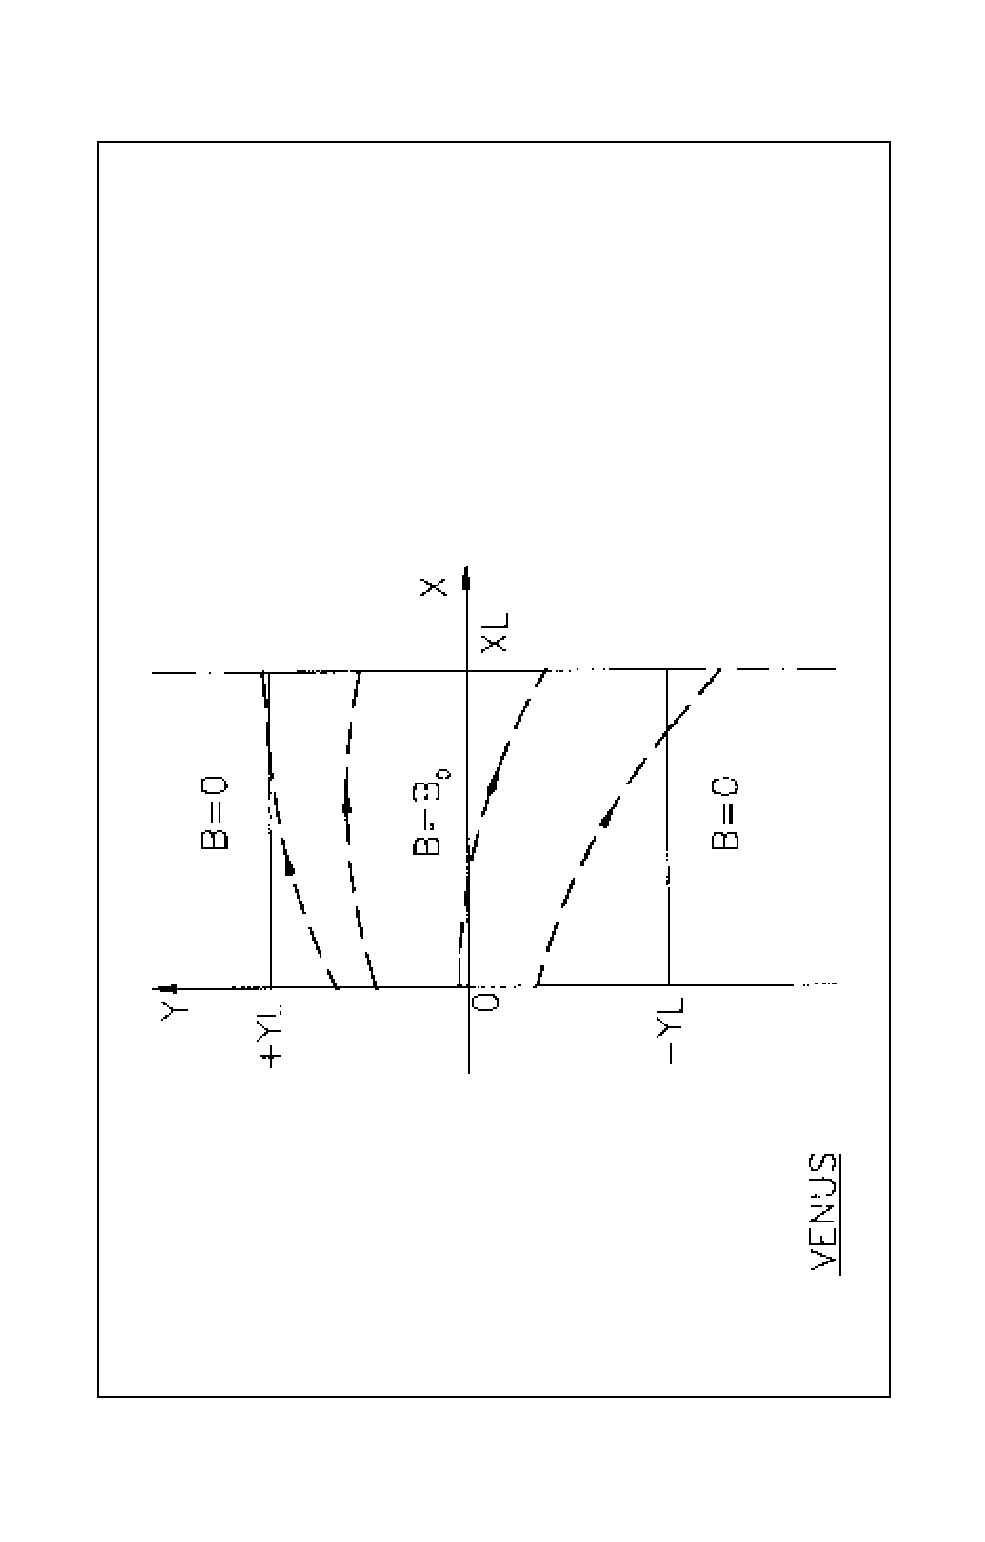
\includegraphics[height=15cm,angle=-90]{Fig32.ps}}
\caption{\label{fig32}Scheme of \textsl{VENUS} rectangular dipole.}
\end{figure}
\vfill

\newpage

\subsubsection*{WIENFILT~: \WIENFILTTitl}\label{WIENFILT} \index{WIENFILT}

\textsl{WIENFILT} simulates a Wien Filter, with transverse and
orthogonal electric and magnetic fields $ \vec  E_Y$,  $ \vec  B_Z $ or $ \vec  E_Z$, 
 $ \vec  B_Y$ (Fig.~\ref{fig28}).
 It must be preceded by \textsl{PARTICUL\index{PARTICUL}} for the definition of particle mass and charge.  
\bigskip

\noindent The length $ \XL $ of the element is the distance between its
entrance and exit EFB's. The electric and magnetic field intensities $ E_0 $ and $ B_0 $ in the 
central, uniform field region, normally satisfy the relation
 
 $$ B_0= - \dfrac{E_0 }{ \beta_ Wc} $$
%
 for the selection of `` wanted''  particles of velocity $\beta_Wc $. Ray-tracing in 
field fall-off regions extends over a distance $ X_E $ $ (X_S) $ beyond the
entrance (exit) EFB by means of prior and further automatic changes of frame. Four sets
of coefficients $\lambda$, $ C_0-C_5 $ allow the description of the entrance and exit fringe 
fields outside the uniform field region, following the model~\cite{Biblio12} %% [12]

\begin{gather*}
	F = \dfrac{1 }{ 1+ \exp(P(s))} \\
	\intertext{where $  P(s) $ is of the term}
	    P(s) = C_0
	       +C_1 \left(  \dfrac{s }{ \lambda} \right) 
	       +C_2 \left( \dfrac{s }{ \lambda} \right)^2 
	       + C_3 \left( \dfrac{s }{ \lambda} \right)^3 
	       +C_4 \left( \dfrac{s }{ \lambda} \right)^4 
	       + C_5 \left(\dfrac{s }{ \lambda} \right)^5 
\end{gather*}
%
and $ s $ is the distance to the EFB.  When fringe fields overlap
inside the element (\emph{i.e.} $ \XL\leq X_E+X_S$),  the field fall-off is expressed as

$$ F = F_E + F_S -1 $$
%
 where $ F_E(F_S) $ is the value of the coefficient respective to the entrance (exit) EFB. 
 
\noindent If $ \lambda_ E=0 $  ($\lambda_ S=0$)  for either the electric or
magnetic component, then both are considered as sharp edge fields and $ X_E(X_S) $ is forced 
to zero (for the purpose of saving computing time).  In this case, the magnetic wedge angle vertical first order focusing effect is simulated at entrance and exit by a kick $P_2 = P_1 - Z_1 \tan (\epsilon / \rho)$ applied to each particle ($P_1$, $P_2$ are the vertical angles upstream and downstream the EFB, $Z_1$ the vertical particle position at the EFB, $\rho$ the local horizontal bending radius and $\epsilon$ the wedge angle experienced by the particle~; $\epsilon$ depends on the horizontal angle T). This is not done for the electric field, however it is advised not to use a sharp edge electric dipole model since this entails non symplectic mapping, and in particular precludes focusing effects of the non zero longitudinal electric field component.

\newpage

\subsubsection*{YMY~: \YMYTitl} \label{YMY} \index{YMY}

\textsl{YMY}  performs a 180$^\circ$ rotation of particle coordinates with respect to the 
$ X $-axis, as shown  in Fig.~\ref{fig33}. 
This is done by means of a change of sign of $ Y $ and $ Z $ axes,  
and therefore coordinates, as follows 

$$ Y2=-Y1,\quad T2=-T1,\quad Z2=-Z1 \quad \text{and} \quad P2=-P1 $$

\vfill
%%%%%%%%%%%%%%figure%%%%%%%%%%%%%%
\begin{figure}[H]
%\vspace{18 truecm}
%%%Figure 33
\centerline{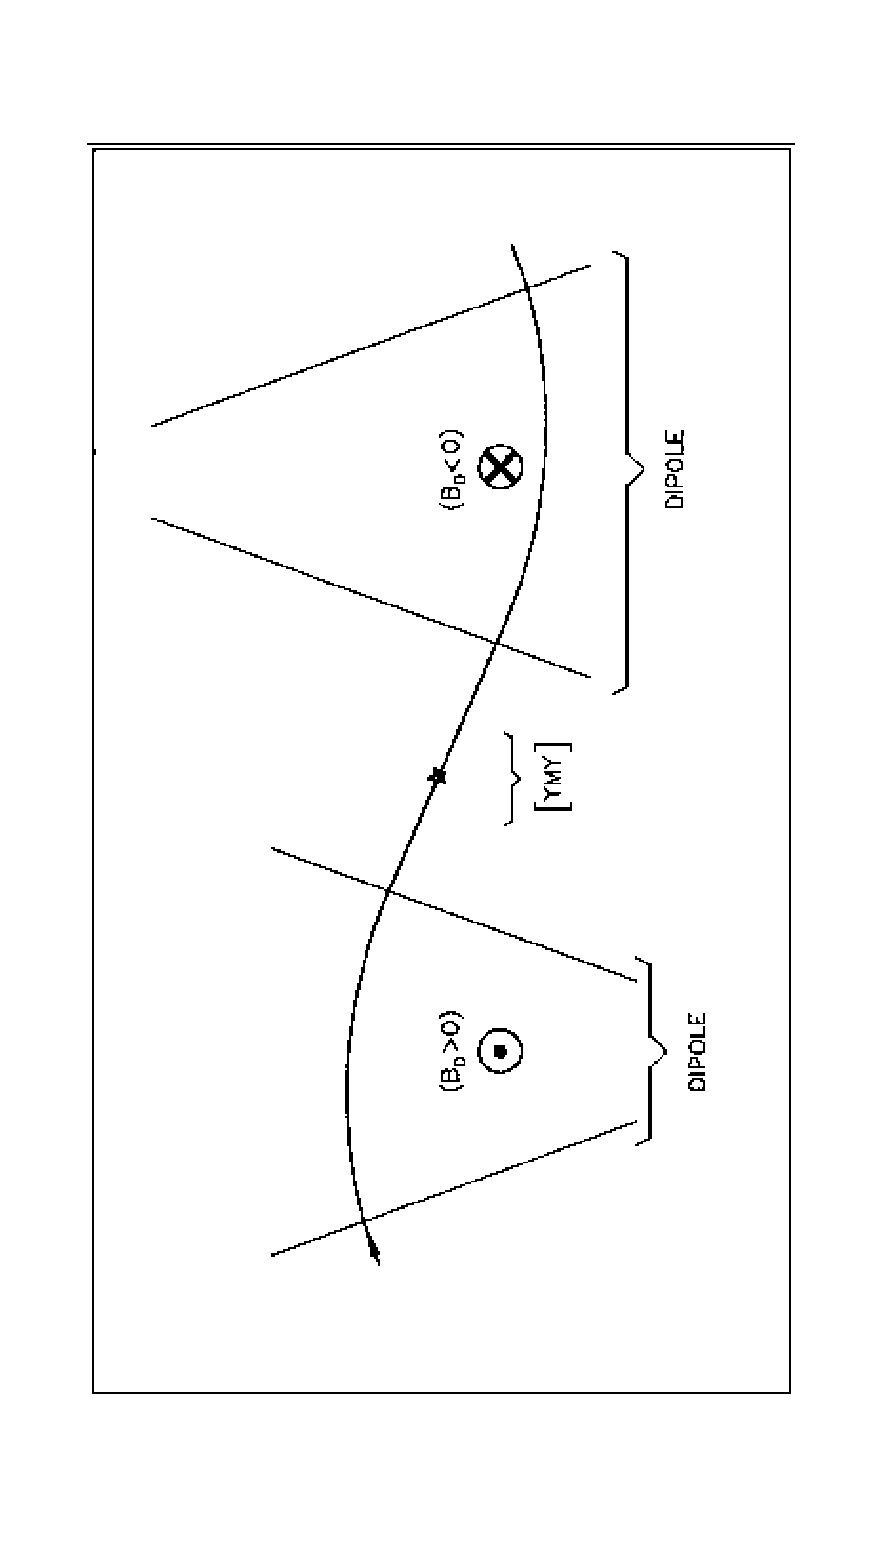
\includegraphics[height=15cm,angle=-90]{Fig33.ps}}
\caption{\label{fig33}\mbox{The use of $ YMY $ in a sequence of two identical
dipoles of opposite signs.}}
\end{figure}
\vfill






\newpage  %%%%% 

\subsection{Output Procedures} \label{sec4.5}

 These procedures are dedicated to the printing of particle coordinates, 
histograms, spin coordinates\index{spin tracking}, etc. They may be called for at any spot in the data pile. 





\newpage

\subsubsection*{FAISCEAU, FAISCNL, FAISTORE~:  Print/Store particle coordinates} \label{FAISCEAU}\label{FAISCNL}
 \label{FAISTORE}\index{FAISCEAU|textbf} \index{FAISCNL|textbf}\index{FAISTORE|textbf}


\textsl{FAISCEAU}  can be introduced anywhere in a structure.  It produces a print  (into zgoubi.res) 
of  initial and actual coordinates of the  \IMAX\index{IMAX@{\IMAX}} particles at the location where it stands, 
together with their tagging indices and letters, following the same format as for \textsl{FAISCNL} (except 
for \textsl{SORT(I)}  which is not printed) .  

\bigskip

\noindent\textsl{FAISCNL} has a similar effect, except that the information is stored in a 
dedicated file \textsl{FNAME} (advised name is \textsl{FNAME} = `zgoubi.fai' 
(formatted write) or `b\_zgoubi.fai' (binary write) \index{zgoubi.fai}
if post-processing with \textbf{zpop}\index{zpop} should follow).  This file may further on be read by means of  \textsl{OBJET}, 
option \mbox{\KOBJ= 3}, or used for other purposes such as graphics (see Part~D of the Guide).  
The data written to that file are formatted and  ordered according to the \FORTRAN sequence 
in the subroutine \textsl{impfai.f}, a copy of which as of Sept.~2009 is as follows~:  

{\footnotesize
\begin{verbatim}
    OPEN (UNIT = NL, FILE = FNAME, STATUS = `NEW')
        DO 1 I=1,IMAX
            P = BORO*CL9 *F(1,I) * AMQ(2,I)
            ENERG = SQRT(P*P + AMQ(1,I)*AMQ(1,I))
            ENEKI = ENERG - AMQ(1,I)
            WRITE(NFAI,110)
     1      LET(I),IEX(I),-1.D0+FO(1,I),(FO(J,I),J=2,MXJ),
     2      -1.D0+F(1,I),F(2,I),F(3,I),
     3      (F(J,I),J=4,MXJ),ENEKI,
     4      I,IREP(I), SORT(I),(AMQ(J,I),J=1,5),RET(I),DPR(I),PS,
     5      BORO, IPASS, KLEY,LBL1,LBL2,NOEL
        ENDDO
 110    FORMAT(1X,1P, 
C1      LET(IT),KEX,      XXXO,(FO(J,IT),J=2,MXJ),
     1  A1, 1X, I2,       7E16.8,
C2        XXX, Y, T*1.D3,
     2  /,3E24.16,
C3      Z,P*1.D3,SAR,     TAR,  ENEKI,
     3         /,4E24.16,E16.8,
C4      IT,IREP(IT), SORT(IT), (AMQ(J,I),J=1,5), RET(IT), DPR(IT), PS,
     4  /,2I6,       9E16.8,
C5      BORO,    IPASS,  KLEY,  (LABEL(NOEL,I),I=1,2),NOEL
     5  /,E16.8, I6,1X,  A8,1X,  2A8,                 I5)
\end{verbatim}}
\medskip

\noindent The meaning of the main data is the following (see the keyword \textsl{OBJET})
\bigskip

{\renewcommand{\arraystretch}{1}
 \begin{tabular}{>{\sl}l!{~:}l}
	$LET(I) $  & one-character string, for tagging particle number $I$  \\
	$IEX\index{IEX@{\IEX}}$, $I$, $IREP(I)$   &  flag, particle number, index  \\
	 $FO(1-6, I)$  &  coordinates $D$, $Y$, $T$, $Z$, $P$ and path
	                 length at the origin of the structure\\
	 $F(1-6, I)$  &  idem, at the current position\\
     $SORT(I)$ & path length at which the particle has possibly been stopped\index{stopped particles}\\
      \multicolumn{1}{c}{  }       & (see \textsl{CHAMBR} or \textsl{COLLIMA})\\
     $RET(I)$, $DPR(I)$ & synchrotron phase space coordinates~; \textsl{RET} =phase (radian),\\
      \multicolumn{1}{c}{  }     &   \textsl{DPR} = momentum dispersion (MeV/c) (see \textsl{CAVITE}) \\
    \textsl{IPASS}  &  turn number (see \textsl{REBELOTE\index{REBELOTE}}) \\
 etc.
     \end{tabular}}
\bigskip

\noindent\textsl{FAISTORE} has an effect similar to \textsl{FAISCNL}, with two more features. 

- On the first data line, \textsl{FNAME} may be followed 
by a series of up to 10 \LABEL's\index{LABEL@{\LABEL}} proper to the elements of the data 
file at the exit of which the print should occur~; if there is no 
label, the print occurs by default at the location of \textsl{FAISTORE}~; if there are labels the 
print occurs right downstream of all optical elements wearing those labels
 (and no longer at the \textsl{FAISTORE} location). 

- The next data line 
gives a parameter, $IP$~: printing will occur every $IP$ other pass, if 
using \REBELOTE\index{REBELOTE} with \textsl{NPASS}\index{NPASS} $ \geq IP-1$. 

For instance the following data input in zgoubi.dat~: 

\medskip

{\renewcommand{\arraystretch}{1}
\begin{tabular}{lll}
	\textsl{FAISTORE} &  &   \\
	zgoubi.fai \index{zgoubi.fai} & \textsl{HPCKUP} & \textsl{VPCKUP}  \\
	12 &  & 
\end{tabular}}
\medskip

\noindent will result in output prints into zgoubi.fai, every 12~other 
pass, each time elements of the zgoubi.dat \index{zgoubi.dat} data list labeled either \textsl{HPCKUP}
or \textsl{VPCKUP} are encountered.

\bigskip

\noindent\underline{Note}

\noindent Binary storage can be obtained from \textsl{FAISCNL} and \textsl{FAISTORE}. This for 
the sake of compactness and access speed, for instance  in case  voluminous amounts of 
data would have to be manipulated. 

This is achieved by giving the storage file a name of the form \textsl{b\_FNAME} 
or \textsl{B\_FNAME}  (e.g., `b\_zgoubi.fai'). The FORTRAN \textsl{WRITE} list 
is the same as in the \textsl{FORMATTED} case above.  

This is compatible with the \textsl{READ} statements in \textbf{zpop} that will recognize binary storage 
from that very radical 'b\_' or 'B\_'. 



\newpage

\subsubsection*{FOCALE, IMAGE[S]~: Particle coordinates and beam size~;  localization and
size  of  horizontal waist}\label{FOCALE}\label{IMAGE}\label{IMAGES}
\index{FOCALE|textbf}\index{IMAGE|textbf}\index{IMAGES|textbf}

\textsl{FOCALE}  calculates the dimensions of the beam and its mean 
transverse position, at a longitudinal distance $ \XL $ from the position 
corresponding to the keyword \textsl{FOCALE}.  
\bigskip

\noindent\textsl{IMAGE}  computes the location and size
of the closest horizontal waist.  
\bigskip

\noindent\IMAGES\index{IMAGES}  has the same effect as \textsl{IMAGE\index{IMAGE}},
 but, in addition, for a 
non-monochromatic beam it calculates as many waists as there are distinct momenta in 
the beam, provided that the object has been defined with a classification of momenta 
(see \textsl{OBJET\index{OBJET}}, \KOBJ = 1, 2  for instance).  
\bigskip

\noindent Optionally, for each of these three procedures, \zgou\ can
list a trace of the coordinates in the $ X$, $Y $ and in the $ Y$, $Z $ planes.  
\bigskip

\noindent The following quantities are calculated for the $ N $ particles of
the beam (\textsl{IMAGE,   FOCALE}) or of each group    of momenta 
(\textsl{IMAGES\index{IMAGES}})  
\bigskip

\begin{itemize}
\item[$\bullet$]Longitudinal position~: 
       \begin{align*}
       \text{\textsl{FOCALE}~:} & \quad  X=\XL  \\
       \text{\textsl{IMAGE[S]}~:} & \quad   X    = - 
    \dfrac{ \sum^ N_{i=1}Y_i\ast tgT_i- 
         \left( \sum^ N_{i=1}Y_i\ast \sum^N_{i=1}tgT_i \right)\, /N }{%
        \sum^ N_{i=1}tg^2T_i- \left( \sum^ N_{i=1}tgT_i\right)^2\, /N} \\ 
            & Y   =   Y_1+X  \ast   \text{tg} T_1  
        \end{align*}    
where $ Y_1 $ and $ T_1 $ are the coordinates of the first particle
of the beam (\textsl{IMAGE, FOCALE}) or the first particle of each group of momenta 
(\textsl{IMAGES\index{IMAGES}}). 

\item[$\bullet$]Transverse position of the center of mass of the waist 
(\textsl{IMAGE[S]}) or of the beam (\textsl{FOCALE}), with respect to the reference trajectory 

$$ YM = \frac{1 }{ N} \sum^ N_{i=1}(Y_i+X  \text{tg} T_i)-Y=
      \frac{1 }{ N} \sum^ N_{i=1}Y\, M_i $$

\item[$\bullet$]FWHM of the image (\textsl{IMAGE[S]}) or of the beam 
(\textsl{FOCALE}), and  total width, respectively, $ W $ and $ WT $

\begin{align*}
	W &   =     2.35 \left( \dfrac{1 }{ N} \sum^ N_{i=1}Y\ M^2_i - Y\ M^2 \right)^{\frac{1}{2}} \\ 
	WT &   =    \max (YM_i)- \min  (YM_i)  
\end{align*}
\end{itemize}

\vfill

\subsubsection*{FOCALEZ, IMAGE[S]Z~: Particle coordinates and beam size~;  localization and 
size  of  vertical waist}\label{FOCALEZ}\label{IMAGEZ}\label{IMAGESZ}
 \index{FOCALEZ|textbf}\index{IMAGEZ|textbf}\index{IMAGESZ|textbf} 
          
Similar to \textsl{FOCALE} and \textsl{IMAGE[S]}, but the calculations are performed 
with respect to the vertical coordinates $ Z_i $ and $ P_i $, in place of $Y_i $ 
and $ T_i$. 
\vfill

\newpage

\subsubsection*{HISTO~: \HISTOTitl}\label{HISTO} \index{HISTO|textbf}
\medskip

Any of the coordinates used in \zgou\ may be histogrammed,
namely initial  $ Y_0$,  $ T_0$,  $ Z_0$,  $ P_0, $ $ S_0 $, $ D_0 $  or actual 
$ Y$, $T$, $Z$, $P$, $S$, $D$ particle coordinates ($ S=$ path length~;  
$ D $ may change  in decay process simulation with \textsl{MCDESINT\index{MCDESINT}}, 
or when ray-tracing in $ \vec  E $ fields), and also spin coordinates\index{spin tracking} and
modulus $ S_X$, $ S_Y$,  $ S_Z $ and $ \left\Vert\vec  S \right\Vert   $.  
\bigskip

\noindent\textsl{HISTO\index{HISTO}}  can be used in conjunction with 
\textsl{MCDESINT\index{MCDESINT}}, for statistics 
on the decay process, by means of \textsl{TYP}.  \textsl{TYP} is a one-character 
variable.  If it is set equal to `S', only secondary particles will be 
histogrammed.  If it is set equal to `P', then only  primary particles will be histogrammed.  
For no discrimination  between S-econdary and P-rimary particles,  \textsl{TYP} = `Q'  must be
used.  
\bigskip

\noindent The dimensions of the histogram (number of lines and columns) may be
modified. It can be normalized with \textsl{NORM} = 1, to avoid saturation.  
\bigskip

\noindent Histograms are indexed with the parameter  $NH$.  This allows making
independent histograms of the same coordinate at several spots  
in a structure.  This is also useful when piling up problems in an input data 
file  (see also \textsl{RESET}). $NH$ is in the range 1-5.  
\bigskip

\noindent If \REBELOTE\index{REBELOTE} is used, the statistics on the $1+$\textsl{NPASS}\index{NPASS}
runs in the structure will add up. 

\vfill
\subsubsection*{IMAGE[S][Z]~: \IMAGESZTitl}

\noindent See FOCALE[Z]. 
\vfill
\newpage

\subsubsection*{MATRIX~: \MATRIXTitl}\label{MATRIX} \index{MATRIX|textbf}
\medskip

\textsl{MATRIX}  causes the calculation of the transfer coefficients of the 
structure, at the spot where it is introduced in the structure, or at the closest horizontal 
focus.  In this last case the position of 
the focus is calculated automatically in the same way as the position of the 
waist in \textsl{IMAGE}. Depending on option \textsl{IFOC},  \textsl{MATRIX} also
delivers the Twiss\index{TWISS} functions, tune numbers, chromaticities\index{Cromaticity|textbf} 
 and other perturbation parameters in the hypothesis of a periodic structure.  


\bigskip

\noindent Depending on the value of option \textsl{IORD}, different procedures follow   

\medskip

\begin{itemize}
\item[$\bullet$] If \textsl{IORD} = 0, \textsl{MATRIX}  is inhibited (equivalent to 
\textsl{FAISCEAU}, whatever \textsl{IFOC}). 

\item[$\bullet$] If \textsl{IORD} = 1, the first order transfer matrix 
$ [R_{ij}]$ is calculated, from a third order expansion of the coordinates. For instance 
$$  Y^+    =   \left( \dfrac{Y}{T_0} \right)\, T_0
	             + \left(\dfrac{Y }{ T^2_0} \right)\, T^2_0 
	             + \left(\dfrac{Y }{ T^3_0} \right)\, T^3_0,   ~ ~ ~ ~ ~ ~ 
	 Y^-    =    - \left(\dfrac{Y }{ T_0} \right)\, T_0 
	             + \left(\dfrac{Y }{ T^2_0} \right)\, T^2_0 -
	             \left(\dfrac{Y }{ T^3_0} \right)\ T^3_0 $$
\noindent will yield, neglecting third order terms, 
$$          R_{11} = \left(\dfrac{Y }{ T_0} \right) = \dfrac{Y^+-Y^- }{ 2T_0} $$


\item[$\bullet$] If \textsl{IORD} = 2, fifth order Taylor expansions are used for the 
calculation of the first order transfer matrix $ [R_{ij}] $ and of 
the second order matrix $[T_{ijk}]$.  Other higher order coefficients are also calculated. 
\end{itemize}

\bigskip

\noindent An automatic generation of an appropriate object for the use of \textsl{MATRIX}  can be obtained 
by means 

\noindent - if  \textsl{IORD} = 1, of the procedure 
\textsl{OBJET}(KOBJ = 5[.I, I=1,9])~(pages~\pageref{OBJET},~\pageref{OBJET-B}),  
that generates sets of up to 9*11 trajectories. In this case, up to nine matrices 
may be calculated, each one wrt. to the reference trajectory of concern as 
indicated using I in KOBJ = 5[.I, I=1,9]~;  

\noindent - if  \textsl{IORD} = 2, of the procedure \textsl{OBJET}(KOBJ = 6)  that generates 
 a set of 61 trajectories. 


\bigskip

\noindent The next option, \textsl{IFOC}, acts as follows \par

\begin{itemize}
\item[$\bullet$] If \textsl{IFOC} = 0,  the transfer coefficients are calculated
at the location of \textsl{MATRIX\index{MATRIX}}, and with respect to the reference trajectory. 
For instance, $ Y^+ $ and $ T^+ $ above are defined for particle number $ i $ as 
$Y^+=Y^+(i)-Y(Ref)$,  and $ T^+=T^+(i)-T(\textrm{ref.})$.  

\item[$\bullet$] If \textsl{IFOC} = 1, the transfer coefficients are calculated at the 
horizontal focus  closest to \textsl{MATRIX\index{MATRIX}} (determined 
automatically), while the reference direction is that of the reference  particle. For 
instance, $ Y^+ $ is defined for particle number $ i $ as $ Y^+=Y^+(i) -Y_{\text{focus}} $, 
while  $ T^+ $ is defined as $ T^+=T^+(i)-T(\textrm{ref.)}$).  

\item[$\bullet$] If \textsl{IFOC} = 2, no change of reference frame is 
performed~: the coordinates refer to the current frame. Namely, $ Y^+=Y^+(i)$, 
$ T^+=T^+(i)$,  etc. \

\paragraph{Periodic structures} 

\item[$\bullet$] If \textsl{IFOC} = 10  +  \textsl{NPeriod}, \textsl{MATRIX\index{MATRIX}} calculates
 periodic parameters characteristic  of the structure 
such as Twiss\index{TWISS} functions and tune numbers, assuming that it is \textsl{NPeriod}-periodic~; 
 no change of reference is performed for these calculations. 
% FM, Nov. 2008
%If  \textsl{IFOC} = 2 additional 
If  \textsl{IORD} = 2 additional 
periodic parameters are computed such as chromaticities\index{Cromaticity}, beta-function momentum dependence, 
 etc. 

These quantities are derived from the first order perturbed and unperturbed transfer 
matrices as obtained in the way described above, and by identification with the Twiss form $ [R_{ij}] 
= I \cos(\mu) + J \sin(\mu)$. 
\end{itemize}

 

\bigskip

\noindent  Addition of \textsl{zgoubi.MATRIX.out} next to \textsl{IORD, IFOC} will cause 
stacking of \textsl{MATRIX} output data 
into   zgoubi.MATRIX.out file (convenient for use with e.g. gnuplot type of data treatment software). 


\newpage

 
\subsubsection*{PICKUPS~: \PICKUPSTitl}\label{PICKUPS} \index{PICKUPS|textbf}
\medskip

\noindent \textsl{PICKUPS} computes the beam centroid path, from average value of particle 
coordinates as observed at \LABEL'ed\index{LABEL@{\LABEL}} keywords.

\medskip
\noindent In conjunction with \textsl{REBELOTE}\index{REBELOTE}, this procedure computes by the same method the closed orbit in 
the periodic structure. 

\medskip
\noindent The \LABEL\ list of concern follows the keyword  \textsl{PICKUPS}.





\newpage


\subsubsection*{PLOTDATA~: \PLOTDATATitl~\protect\cite{BiblioPlot}}%
\label{PLOTDATA} \index{PLOTDATA}

\bigskip

\noindent {\it To be documented}

\newpage

\subsubsection*{SPNPRNL, SPNSTORE, SPNPRT~: Print/Store spin coordinates 
  }\label{SPNPRT}\label{SPNPRNL} \label{SPNSTORE}
\index{SPNPRT}\index{SPNPRNL}\index{SPNSTORE}

\noindent \textsl{SPNPRT} can be introduced anywhere in a structure. It produces
a listing (into zgoubi.res) of the initial and actual coordinates and modulus of the spin of the \IMAX\index{IMAX@{\IMAX}}
particles, at the location where it stands, together with their Lorentz factor $\gamma$, etc. 
The mean values of the spin components are also printed. 

\bigskip

\noindent \textsl{SPNPRNL} has similar effect to \textsl{SPNPRT}, except that the information is
stored in a  dedicated file \textsl{FNAME} (should post-processing with \textbf{zpop}\index{zpop} follow, 
advised name is \textsl{FNAME} = `zgoubi.spn' (formatted write) or `b\_zgoubi.spn' (binary write) \index{zgoubi.spn}). 
The data are formatted and ordered according to the  \FORTRAN sequence found in the subroutine \textsl{spnprn.f}, 
with meaning of printed quantities as follows~: 

\medskip

 \begin{tabular}{>{\sl}l!{~:}l}
	 LET(I),IEX(I)\index{IEX@{\IEX}}  &  tagging character and flag (see \textsl{OBJET}) \\
	 SI(1-4,I) & spin components\index{spin tracking} $SX$, $SY$, $SZ$  and modulus, at the origin\\
	 SF(1-4,I)   &  idem, at the current position\\
	  GAMMA &   Lorentz relativistic factor\\
	  I  &  particle number\\
	 IMAX &  total number of particles ray-traced (see  \textsl{OBJET})\\
	 IPASS &  turn number (see \textsl{REBELOTE})\\
 \end{tabular}

\bigskip

\noindent\textsl{SPNSTORE} has an effect similar to \textsl{SPNPRNL}, with two more features. 

- On the first data line, \textsl{FNAME} may be followed 
by a series of up to 10 \LABEL's\index{LABEL@{\LABEL}} proper to the elements of the zgoubi.dat data 
file at the exit of which the print should occur~; if no label is given, 
the print occurs by default at the very location of \textsl{SPNSTORE}~; 
if there  label(s) is (are) given
print occurs right downstream of all optical elements wearing those labels
 (and no longer at the \textsl{SPNSTORE} location). 

- The next data line 
gives a parameter, $IP$~: printing will occur every $IP$ other pass, when 
using \REBELOTE\index{REBELOTE} with \textsl{NPASS}\index{NPASS} $ \geq IP-1$. 

For instance the following data input in zgoubi.dat~: 

\medskip

{\renewcommand{\arraystretch}{1}
\begin{tabular}{lll}
	\textsl{SPNSTORE} &  &   \\
	zgoubi.spn \index{zgoubi.fai} & \textsl{HPCKUP} & \textsl{VPCKUP}  \\
	12 &  & 
\end{tabular}}
\medskip

\noindent will result in output prints into zgoubi.spn, every 12~other 
pass, each time elements of the zgoubi.dat \index{zgoubi.dat} data list labeled either \textsl{HPCKUP}
or \textsl{VPCKUP} are encountered.

\bigskip

\noindent\underline{Note}

\noindent Binary storage can be obtained from \textsl{SPNPRNL} and \textsl{SPNSTORE}. This for 
the sake of compactness and I/O access speed by zgoubi  or zpop, for instance  in case  voluminous amounts of 
data should be manipulated. 

This is achieved by giving the storage file a name of the form \textsl{b\_FNAME} 
or \textsl{B\_FNAME}  (e.g., `b\_zgoubi.spn'). The FORTRAN \textsl{WRITE} ouput list 
is the same as in the \textsl{FORMATTED} case above.  





\newpage

\subsubsection*{SRPRNT~: \SRPRNTTitl}\label{SRPRNT}\index{SRPRNT|textbf}\index{synchrotron radiation loss}

\noindent\textsl{SRPRNT} may be introduced anywhere in a structure. It produces
a listing (into zgoubi.res) of current state of statistics on several parameters related to 
SR loss  presumably  activated beforehand with keyword \textsl{SRLOSS}. 

 \newpage


\subsubsection*{TWISS~: \TWISSTitl}\label{TWISS} \index{TWISS|textbf}
\medskip

\textsl{TWISS}  
causes the calculation of 
  transfer coefficients and various other parameters, in particular 
periodical quantities  such as tunes, chromaticies\index{Cromaticity}, etc. 

\noindent If \textsl{KTWISS} = 1, the object necessary for these calculations 
    can be generated automatically by means of \textsl{OBJET\index{OBJET}}  with
option \mbox{\KOBJ= 5}.   
When using 
\textsl{KTWISS} = 2, the object can be generated automatically with \textsl{OBJET}  and 
 \mbox{\KOBJ=  6}. 

 
\newpage




\subsection{Complementary Features} \label{sec4.6}  

\subsubsection{Backward Ray-tracing} \label{sec4.6.3} 
\index{backward ray-tracing} \index{XPAS, negative}\index{integration step size!negative}

For the purpose of parameterization for instance, it may be interesting to ray-trace 
backward  from the image toward the object.  This can be performed by first 
reversing the position of optical elements in the structure, and then 
reversing the integration step sign in all the optical elements.  
\bigskip

\noindent An illustration of this feature is given in the following
Figure~\ref{fig36}.    


%%%%%%%%%%%%%%figure%%%%%%%%%%%%%%
\begin{figure}[H]
%\vspace{16 truecm}
%%%Figure 36
\centerline{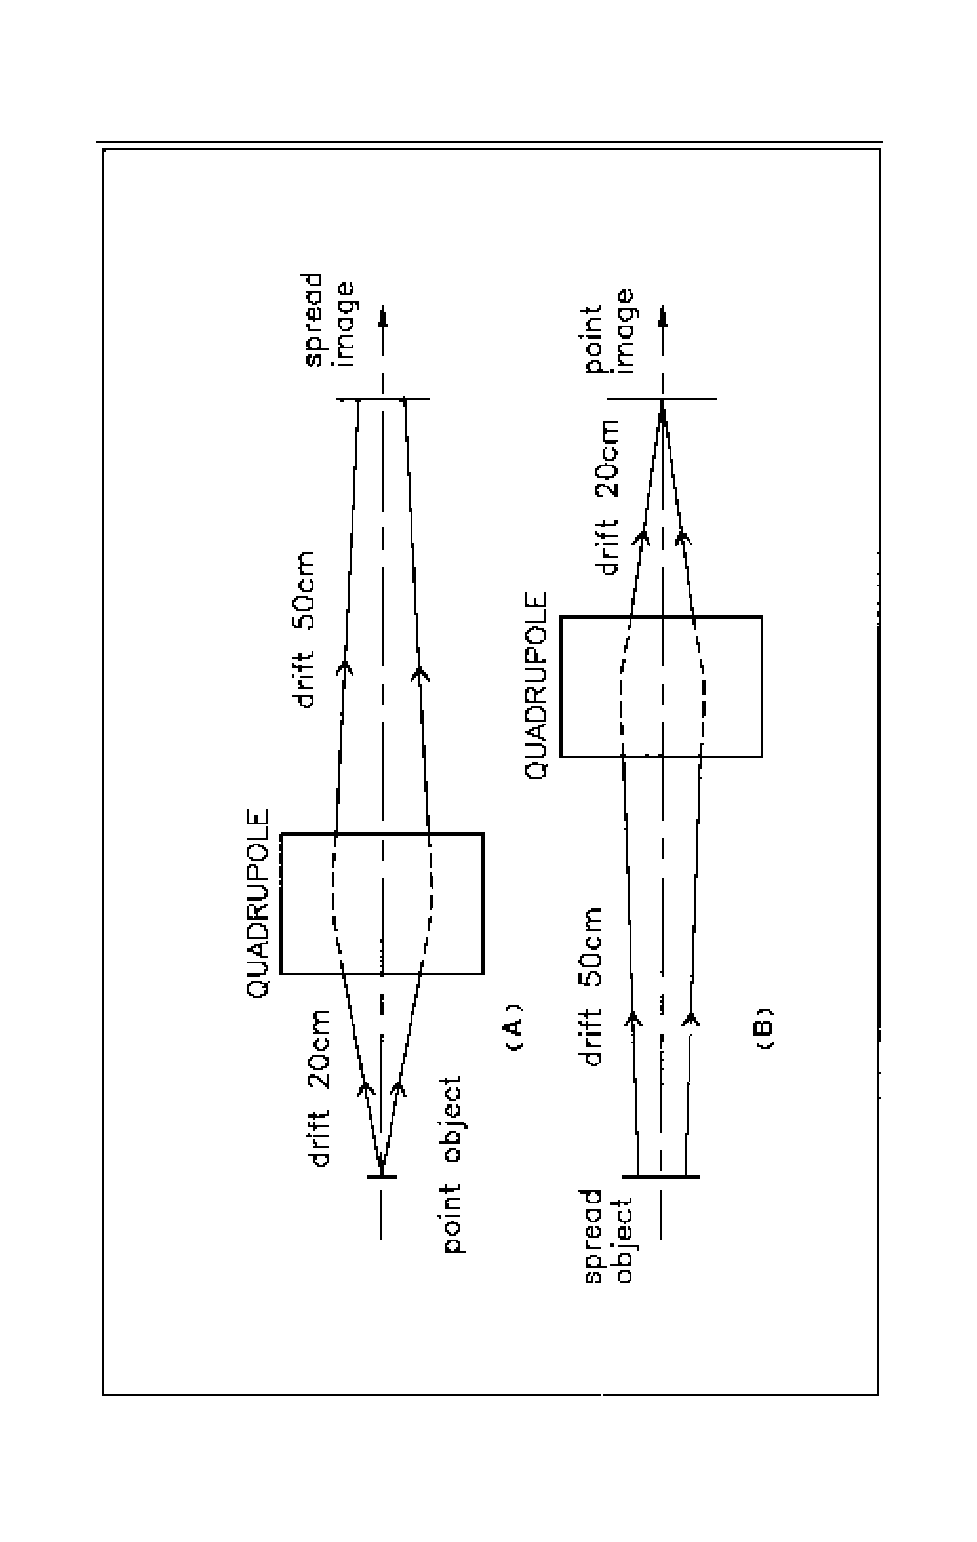
\includegraphics[height=12cm,angle=-90]{Fig36.ps}}
\hangcaption[Fig36]{\label{fig36}A. Regular forward ray-tracing, from object to image.\\
B. Same  structure, with backward ray-tracing from image to object~: negative integration step XPAS is used in  the quadrupole.}
\end{figure}


\subsubsection{Checking Fields and Trajectories inside Optical Elements}  \label{sec4.6.1}
\index{checking field}\index{checking trajectories}

In all optical elements, an option index $ \IL $\index{IL@{\IL}} is available.  It
is normally set to 0 and in this case has no effect.

\noindent $ \IL=1 $ causes a print  in zgoubi.res \index{zgoubi.res} of particle 
coordinates and field
along trajectories in the optical element.  In the meantime, a calculation and summation of
the values of $ \vec  \nabla \cdot\vec  B$, 
 $ \vec  \nabla \times\vec  B $ and $ \nabla^2\vec  B $ (same for $\vec E$) at all 
integration steps is performed, which allows a check of the behavior of 
$ \vec  B $ (or $ \vec  E $) in field maps (all these derivatives should normally be zero).

\noindent $ \IL=2 $ causes a print   of particle coordinates and other 
informations in zgoubi.plt\index{zgoubi.plt} at each integration step~; this information 
 can further be processed with 
\textbf{zpop}\footnote{See Part D of the Guide.}\index{zpop}. In order to limit the volume of 
that storage file (when dealing with small step size, large number of particles, etc.) it is possible 
to print out  every other $10^n$ integration step by taking $ \IL=2 \times 10^n $ (for instance, 
 $ \IL=200 $ would cause output into zgoubi.plt every $100$ other step). 
\bigskip

\noindent When dealing with maps (e.g., \textsl{CARTEMES\index{CARTEMES}}, \textsl{ELREVOL
\index{ELREVOL}}), another option index $ \IC $\index{IC@{\IC}} is available.
  It is normally set to 0 and in this case has no effect.
 
\noindent $ \IC=1 $ causes a print of the field map in zgoubi.res. \index{zgoubi.res}

\noindent $ \IC=2 $ will cause a print   of field maps in zgoubi.map \index{zgoubi.map}
which can further be processed with \textbf{zpop}. 
%%%%%%%\addtocounter{footnote}{-1}\footnotemark.

\newpage

 \subsubsection{Labeling keywords}\label{sec4.6.8}\index{LABEL@{\LABEL}|textbf}

Keywords in \zgou\ data file zgoubi.dat can be \LABEL'ed, for the purpose of 
the execution of such procedures as  \textsl{PICKUPS}\index{PICKUPS}, \textsl{FAISCNL}, \textsl{FAISTORE}
\index{FAISCNL}\index{FAISTORE}, \textsl{SCALING}\index{SCALING}, and also for the purpose of 
particle coordinate storage into zgoubi.plt\index{zgoubi.plt} (see Sections~\ref{sec4.6.1} 
and \ref{secD-3}). 

\noindent Each keyword accepts two \LABEL's, of which the first one is used for the 
above mentioned purposes. The keyword and related \LABEL['s] should fit within a 80-character 
long string on a single line. 

\subsubsection{Multiturn tracking in circular machines} \label{sec4.6.5}

Multiturn\index{multiturn} tracking  in circular machines can be performed by
means of the keyword \textsl{REBELOTE\index{REBELOTE}}, put at the end of the optical structure 
with its argument \textsl{NPASS}$+1$\index{NPASS} being the number of turns to be 
performed. In order that the \IMAX\index{IMAX@{\IMAX}} particles of the beam start a new 
turn with the coordinates they have reached at the end of the 
previous one, the option $ K=99 $ has to be specified in \textsl{REBELOTE\index{REBELOTE}}.
\bigskip

\noindent\textbf{Synchrotron acceleration} can be simulated, following the 
procedure below  
\begin{itemize}
\item[-] \textsl{CAVITE\index{CAVITE}} appears at the end of the structure (before
\textsl{REBELOTE\index{REBELOTE}}), with option \textsl{IOPT}$=1$ 

\item[-] the R.F.\ frequency of the cavity is given a timing law by 
means of \textsl{SCALING\index{SCALING}}, family \textsl{CAVITE}

\item[-] the magnets are given the same timing law $ \Br (T)$,  
(where $T=1 $ to \textsl{NPASS}$+1$ is the turn number) by means of \textsl{SCALING}. \par
\end{itemize}

\noindent Eventually some families of magnets may be given a law which does 
not follow $ \Br (T)$,  for the simulation of special processes (e.g.\ 
fast crossing of spin resonances with independent families of 
quadrupoles). 

%\noindent This is illustrated in the example~6 of Part~C.  %%%% ref




\subsubsection{Positioning\index{Positioning|textbf}, (mis-)alignement\index{Misalignement|textbf}, 
of optical elements  and field maps} \label{sec4.6.2} 

The last record in most optical elements and field maps is the positioning flag 
\textsl{KPOS}\index{KPOS|textbf}, followed by the parameterss \textsl{XCE}, \textsl{YCE} 
for translation and \textsl{ALE} for rotation. The positioning works in two different ways, 
depending  whether they are defined in 
Cartesian $ (X, Y, Z) $ coordinates (e.g., \textsl{QUADRUPO\index{QUADRUPO}, TOSCA\index{TOSCA}}),
 or polar 
 ($R$, $\theta$, $Z$)  coordinates (\textsl{DIPOLE\index{DIPOLE}}). 
 
 \subsubsection*{Cartesian Coordinates~:} 
 
 If \textsl{KPOS} $ =1$, the optical element is moved (shifted by \textsl{XCE, YCE} and Z-rotated by 
\textsl{ALE}) with respect to the incoming reference frame. Trajectory coordinates after traversal of the 
element refer the element frame. 

\noindent If  \textsl{KPOS} $=2 $, the shifts   \textsl{XCE}\index{XCE}   
and   \textsl{YCE}\index{YCE}, and the tilt angle \textsl{ALE}\index{ALE@{\it ALE}}   are taken into 
account, for mis-aligning  the element with respect to the incoming 
reference, as shown in Fig.~\ref{fig34}.  
The effect is equivalent to  a \textsl{CHANGREF(XCE,YCE,ALE)}  upstream of the 
optical element, followed by   \textsl{CHANGREF(XCS,YCS,ALS=-ALE)} downstream of it, with 
 computed \textsl{XCS, YCS} values as schemed in Fig.~\ref{fig34}.  

\noindent \textsl{KPOS} $=3 $ option is available for some 
 magnets  (e.g., \textsl{BEND}, \textsl{MULTIPOL})~; 
it is effective only if a non zero dipole component $B1$ is present, or if  \textsl{ALE} is non-zero. 
It positions automatically the 
device in the  following way, convenient for periodic structures (Fig~\ref{figKPOS3}).
 
Both incoming and outgoing refernce frames are  tilted w.r.t. the magnet 

 $\bullet$ either,  by an angle \textsl{ALE}  if ALE$\not =$0, 

 $\bullet$ or, if ALE=0  by  half the deviation $\theta/2$ (such that $ L = 
2 \frac{\BORO}{B1} \sin({\theta}/{2})$ wherein L = geometrical length, 
\BORO  = reference rigidity as defined in \textsl{OBJET\index{OBJET}}).
%\noindent This is equivalent to the sequence \textsl{CHANGREF(0,0,-$\theta$/2)},
%  \textsl{CHANGREF(0,YCE,0)} right upstream the magnet, followed  by 
%\textsl{CHANGREF(0,-YCE,-$\theta$/2)}.

\noindent Next, the optical element is  shifted by \textsl{Y-shift=YCE} (\textsl{XCE} is not used) in a 
direction orthogonal to the new magnet axis (i.e., at an angle $ALE+\pi/2$ wrt. the incoming 
reference frame $X$-axis). 


%%%%%%%%%%%%%%figure%%%%%%%%%%%%%%
\vfill

\begin{figure}[H]
\begin{center}
%\begin{minipage}{.45\linewidth}
%\begin{center}

\mbox{
\includegraphics[height=4cm]{Fig34A.eps}
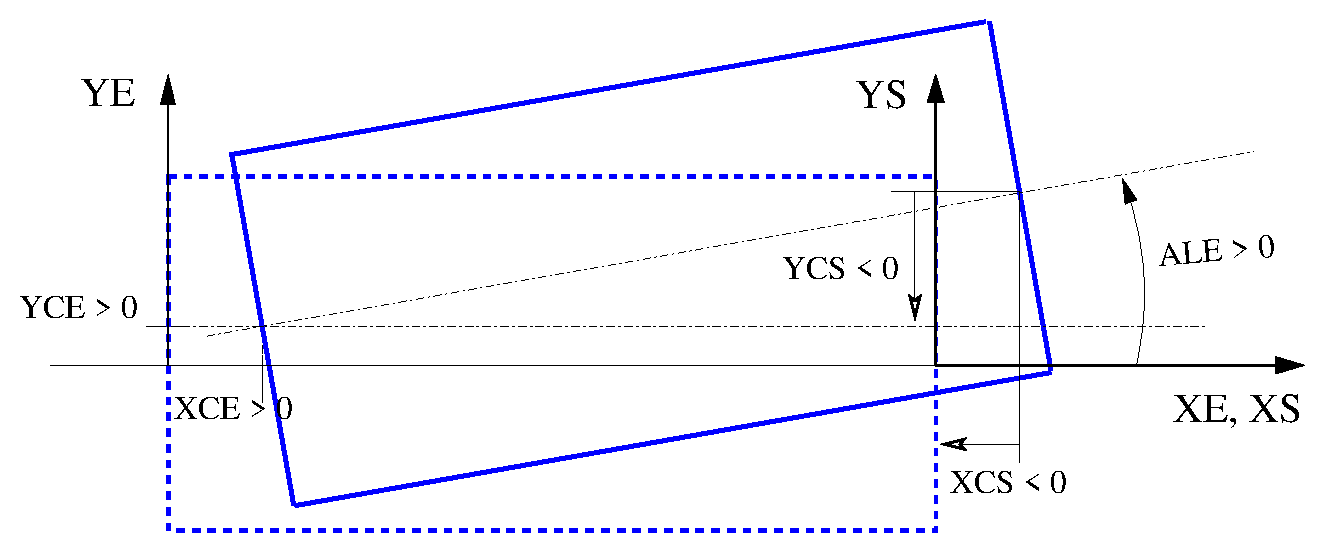
\includegraphics[height=3.5cm]{Fig34.eps}
}
\hangcaption{\label{fig34} 
  Left~: moving an optical element using  \textsl{KPOS}$=1 $. 
Right~: Mis-aligning  an optical element using  \textsl{KPOS}$=2 $.  
\textsl{$(X_E,Y_E)$} and \textsl{$(X_S, Y_S)$} are respectively the incoming 
 and outgoing  reference frames.
}
%\end{center}
%\end{minipage}  %\hspace{.05\linewidth}
%\begin{minipage}{.45\linewidth}
%\begin{center}

~

~

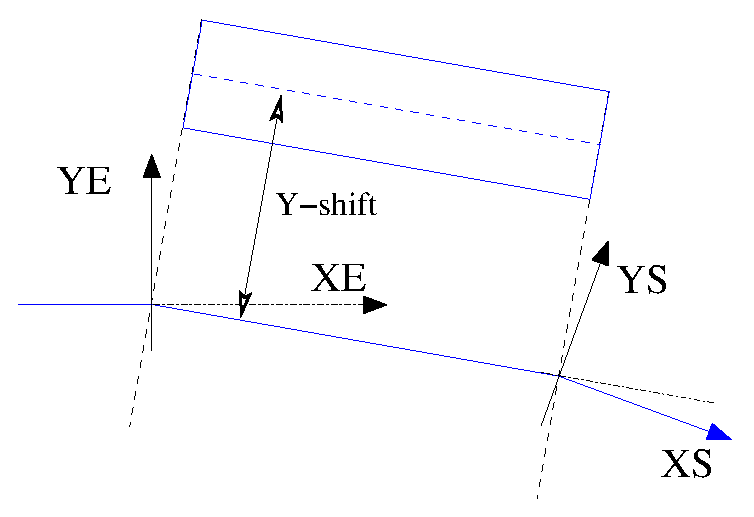
\includegraphics[height=5cm]{FigKPOS3.eps}

\hangcaption{\label{figKPOS3} 
Half-deviation alignement of a Cartesian coordinate bending element, 
using  \textsl{KPOS}$=3 $.  \textsl{$(X_E,Y_E)$} and \textsl{$(X_S, Y_S)$} are respectively the incoming 
 and outgoing  reference frames.
}
%\end{center}
%\end{minipage}
%\end{center}
%\end{figure}
%%%%%%%%%%%%%%figure%%%%%%%%%%%%%%
%\begin{figure}
%\vspace{12 truecm}
%%%Figure 35

~

~

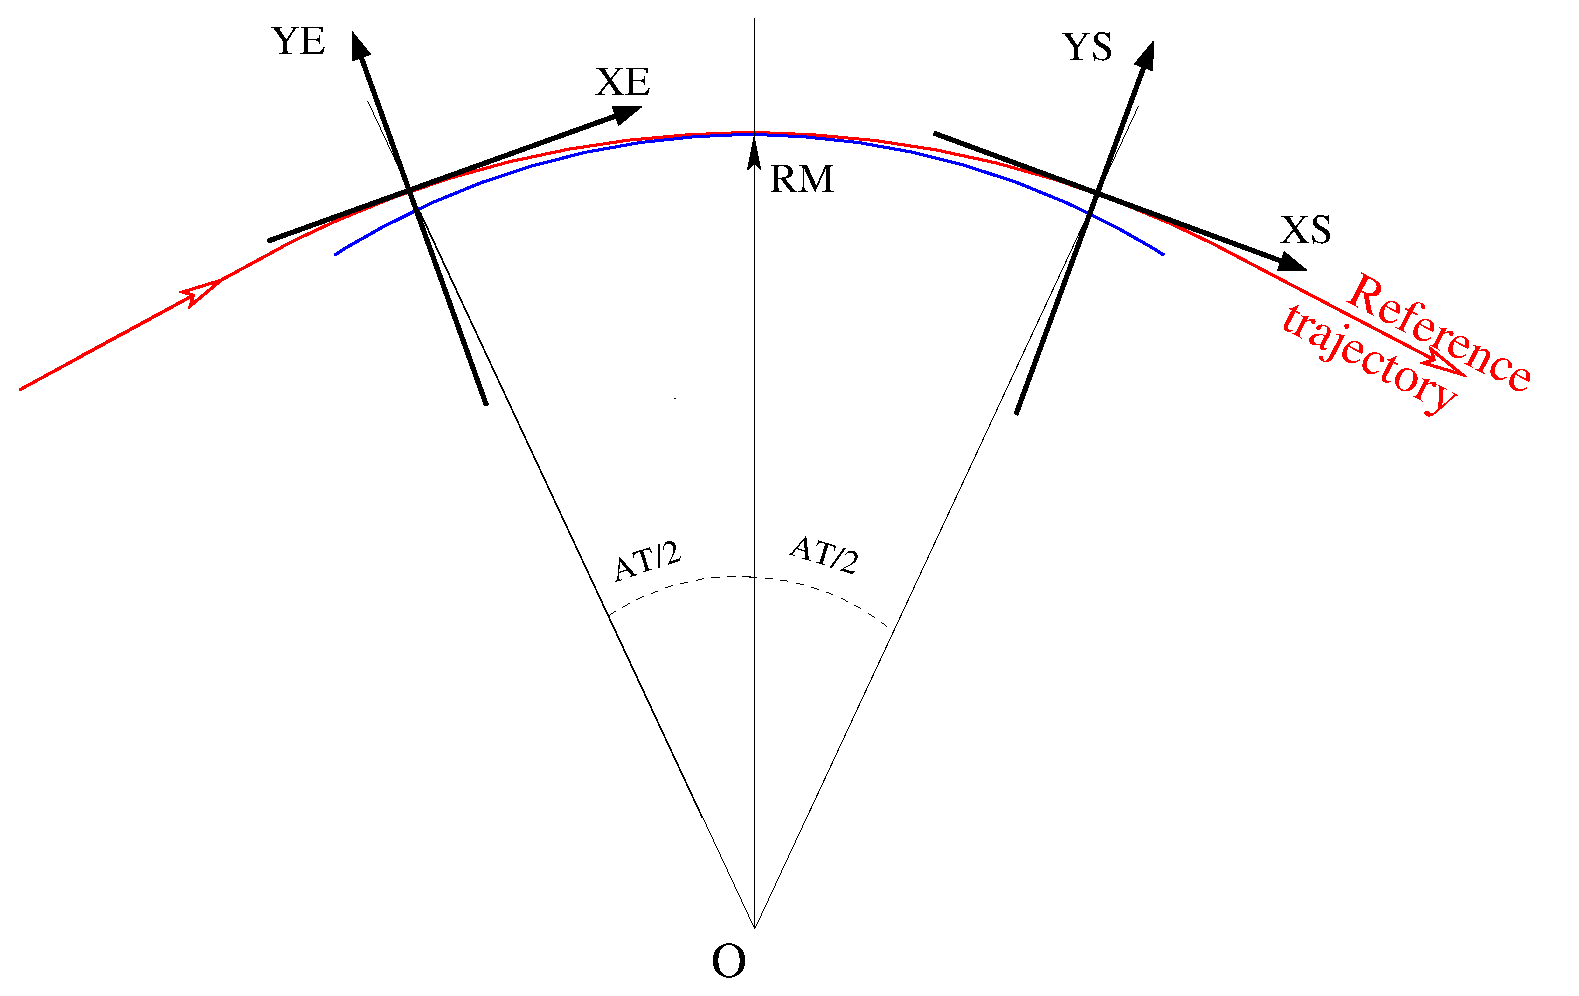
\includegraphics[height=6cm]{Fig35.eps}
\hangcaption{\label{fig35}Positioning of a polar field map, using \textsl{KPOS}$=1 $.}
\end{center}
\end{figure}


\clearpage 

 \subsubsection*{Polar Coordinates} 
 
 If  \textsl{KPOS} $=1$,  the element is positioned automatically in such a way
that a particle entering with zero initial coordinates and 
$ 1+DP=\Br /\BORO $ 
relative momentum will reach position ($ RM$, $\frac{AT }{ 2} $) in 
the element with $ T=0 $ angle with respect to the moving frame in the polar 
coordinates system of the element (Fig.~\ref{fig35}~; 
see \textsl{DIPOLE-M\index{DIPOLE-M}} and \textsl{POLARMES\index{POLARMES}}).

\noindent If  \textsl{KPOS} $=2, $ the map is positioned in such a way that the 
incoming reference frame is presented  at radius $ RE $ with angle $ TE $.  
The exit reference frame of \zgou\  is positioned in a similar way with 
respect to the map,  by means of 
the two parameters $ RS $ (radius) and $ TS $ (angle) (see Fig.~\ref{fig9}A.).  






 \subsubsection{Coded integration step\index{XPAS, coded}\index{integration step size!coded}} 

In several optical elements (e.g., all multipoles, \textsl{BEND}) the 
integration step (in general noted \textsl{XPAS}) can be coded under the 
form \textsl{XPAS} = \texttt{\#E|C|S}, where \texttt{E} is the number of
steps taken in the entrance fringe field, \texttt{C} is the number of
steps in the magnet body, and \texttt{S} is the number of steps in the 
exit fringe field.

\subsubsection{Ray-tracing of an arbitrarily large number of particles} %
      \label{sec4.6.4}

Monte Carlo\index{Monte Carlo} multiparticle \index{multiparticle} simulations involving an 
arbitrary number of particles
can be performed by means of \textsl{REBELOTE\index{REBELOTE}}, put at the end of the optical
structure, with its argument \textsl{NPASS}\index{NPASS} being the number of passes through 
\textsl{REBELOTE\index{REBELOTE}}, and (\textsl{NPASS}$+ 1$) * \IMAX\index{IMAX@{\IMAX}}  
the number of particles to 
be ray-traced. In order that new initial conditions  ($D$, $Y$, $T$, $Z$, 
$P$, $X$) 
 be generated at each pass, $ K=0 $ has to be specified in \textsl{REBELOTE\index{REBELOTE}}.
 
\noindent Statistics on coordinates, spins\index{spin tracking}, and other histograms can be
performed by means of such procedures as \textsl{HISTO\index{HISTO}, SPNTRK\index{SPNTRK}}, 
etc. that stack the information from pass to pass. 


\subsubsection{Stopped particles~: the \IEX\ flag} 
\label{sec4.6.6}\index{stopped particles}\index{IEX@{\IEX}|textbf}

As described in \textsl{OBJET\index{OBJET}}, each particle $I=1$, \IMAX\
 is attached a
value $IEX(I)$ of the \IEX\ flag. Normally, $IEX(I)=1$. Under certain 
circumstances, \IEX\ may take negative values, as follows

\begin{itemize}
\item[$-1$]~:  the trajectory happened to wander outside the limits of a field map 
\item[$-2$]~:  too many integration steps\index{integration step size} in an optical element
\item[$-3$]~:  deviation happened to exceed $\dfrac{\pi}{2} $ in an optical element 
\item[$-4$]~:  stopped by walls (procedures \textsl{CHAMBR, COLLIMA})  
\item[$-5$]~:  too many iterations in subroutine \textsl{DEPLA}  
\item[$-6$]~:  energy loss exceeds particle energy 
\item[$-7$]~:  field discontinuities larger than 50\% wthin a field map
\item[$-8$]~:  reached field limit in an optical element
\end{itemize}


\noindent Only in the case $IEX=-1$ will the integration not be stopped since in this case 
the field outside the map is extrapolated from the map data, and the particle may possibly get 
back into the map (see section~\ref{sec2.4.2} on page~\pageref{sec2.4.2}).  In all other cases 
  the particle of concern will be stopped. 

\subsubsection{Negative rigidity} \label{sec4.6.7}  \index{negative rigidity} 
\index{negative charge}\index{negative momentum}

\zgou\ can handle negative rigidities $\Br = p/q$. This is equivalent to 
considering either particles of negative charges ($q<0$), or counter 
going particles ($p<0$), or virtually reversed fields (w.r.t.~the field sign 
that shows in the optical element data list).

\noindent Negative rigidities may be specified in terms of 
\BORO $<0$ or $D=\Br / \BORO < 0$ when 
defining the initial coordinates with \textsl{OBJET}\index{OBJET} and 
\textsl{MCOBJET}\index{MCOBJET}.
